\documentclass[journal,12pt,twocolumn]{IEEEtran}
%
\usepackage{setspace}
\usepackage{gensymb}
%\doublespacing
\singlespacing

%\usepackage{graphicx}
%\usepackage{amssymb}
%\usepackage{relsize}
\usepackage[cmex10]{amsmath}
%\usepackage{amsthm}
%\interdisplaylinepenalty=2500
%\savesymbol{iint}
%\usepackage{txfonts}
%\restoresymbol{TXF}{iint}
%\usepackage{wasysym}
\usepackage{amsthm}
\usepackage{iithtlc}
\usepackage{mathrsfs}
\usepackage{txfonts}
\usepackage{stfloats}
\usepackage{bm}
\usepackage{cite}
\usepackage{cases}
\usepackage{subfig}
%\usepackage{xtab}
\usepackage{longtable}
\usepackage{multirow}
%\usepackage{algorithm}
%\usepackage{algpseudocode}
\usepackage{enumitem}
\usepackage{mathtools}
\usepackage{tikz}
\usepackage{circuitikz}
\usepackage{verbatim}
\usepackage{tfrupee}
\usepackage[breaklinks=true]{hyperref}
%\usepackage{stmaryrd}
\usepackage{tkz-euclide} % loads  TikZ and tkz-base
\usetkzobj{all}
\usepackage{listings}
    \usepackage{color}                                            %%
    \usepackage{array}                                            %%
    \usepackage{longtable}                                        %%
    \usepackage{calc}                                             %%
    \usepackage{multirow}                                         %%
    \usepackage{hhline}                                           %%
    \usepackage{ifthen}                                           %%
  %optionally (for landscape tables embedded in another document): %%
    \usepackage{lscape}     
\usepackage{multicol}
\usepackage{chngcntr}
%\usepackage{enumerate}

%\usepackage{wasysym}
%\newcounter{MYtempeqncnt}
\DeclareMathOperator*{\Res}{Res}
%\renewcommand{\baselinestretch}{2}
\renewcommand\thesection{\arabic{section}}
\renewcommand\thesubsection{\thesection.\arabic{subsection}}
\renewcommand\thesubsubsection{\thesubsection.\arabic{subsubsection}}

\renewcommand\thesectiondis{\arabic{section}}
\renewcommand\thesubsectiondis{\thesectiondis.\arabic{subsection}}
\renewcommand\thesubsubsectiondis{\thesubsectiondis.\arabic{subsubsection}}

% correct bad hyphenation here
\hyphenation{op-tical net-works semi-conduc-tor}
\def\inputGnumericTable{}                                 %%

\lstset{
%language=C,
frame=single, 
breaklines=true,
columns=fullflexible
}
%\lstset{
%language=tex,
%frame=single, 
%breaklines=true
%}

\begin{document}
%


\newtheorem{theorem}{Theorem}[section]
\newtheorem{problem}{Problem}
\newtheorem{proposition}{Proposition}[section]
\newtheorem{lemma}{Lemma}[section]
\newtheorem{corollary}[theorem]{Corollary}
\newtheorem{example}{Example}[section]
\newtheorem{definition}[problem]{Definition}
%\newtheorem{thm}{Theorem}[section] 
%\newtheorem{defn}[thm]{Definition}
%\newtheorem{algorithm}{Algorithm}[section]
%\newtheorem{cor}{Corollary}
\newcommand{\BEQA}{\begin{eqnarray}}
\newcommand{\EEQA}{\end{eqnarray}}
\newcommand{\define}{\stackrel{\triangle}{=}}

\bibliographystyle{IEEEtran}
%\bibliographystyle{ieeetr}


\providecommand{\mbf}{\mathbf}
\providecommand{\pr}[1]{\ensuremath{\Pr\left(#1\right)}}
\providecommand{\qfunc}[1]{\ensuremath{Q\left(#1\right)}}
\providecommand{\sbrak}[1]{\ensuremath{{}\left[#1\right]}}
\providecommand{\lsbrak}[1]{\ensuremath{{}\left[#1\right.}}
\providecommand{\rsbrak}[1]{\ensuremath{{}\left.#1\right]}}
\providecommand{\brak}[1]{\ensuremath{\left(#1\right)}}
\providecommand{\lbrak}[1]{\ensuremath{\left(#1\right.}}
\providecommand{\rbrak}[1]{\ensuremath{\left.#1\right)}}
\providecommand{\cbrak}[1]{\ensuremath{\left\{#1\right\}}}
\providecommand{\lcbrak}[1]{\ensuremath{\left\{#1\right.}}
\providecommand{\rcbrak}[1]{\ensuremath{\left.#1\right\}}}
\theoremstyle{remark}
\newtheorem{rem}{Remark}
\newcommand{\sgn}{\mathop{\mathrm{sgn}}}
\providecommand{\abs}[1]{\left\vert#1\right\vert}
\providecommand{\res}[1]{\Res\displaylimits_{#1}} 
\providecommand{\norm}[1]{\left\lVert#1\right\rVert}
%\providecommand{\norm}[1]{\lVert#1\rVert}
\providecommand{\mtx}[1]{\mathbf{#1}}
\providecommand{\mean}[1]{E\left[ #1 \right]}
\providecommand{\fourier}{\overset{\mathcal{F}}{ \rightleftharpoons}}
%\providecommand{\hilbert}{\overset{\mathcal{H}}{ \rightleftharpoons}}
\providecommand{\system}{\overset{\mathcal{H}}{ \longleftrightarrow}}
	%\newcommand{\solution}[2]{\textbf{Solution:}{#1}}
\newcommand{\solution}{\noindent \textbf{Solution: }}
\newcommand{\cosec}{\,\text{cosec}\,}
\providecommand{\dec}[2]{\ensuremath{\overset{#1}{\underset{#2}{\gtrless}}}}
\newcommand{\myvec}[1]{\ensuremath{\begin{pmatrix}#1\end{pmatrix}}}
\newcommand{\mydet}[1]{\ensuremath{\begin{vmatrix}#1\end{vmatrix}}}
%\numberwithin{equation}{section}
\numberwithin{equation}{subsection}
%\numberwithin{problem}{section}
%\numberwithin{definition}{section}
\makeatletter
\@addtoreset{figure}{problem}
\makeatother

\let\StandardTheFigure\thefigure
\let\vec\mathbf
%\renewcommand{\thefigure}{\theproblem.\arabic{figure}}
\renewcommand{\thefigure}{\theproblem}
%\setlist[enumerate,1]{before=\renewcommand\theequation{\theenumi.\arabic{equation}}
%\counterwithin{equation}{enumi}


%\renewcommand{\theequation}{\arabic{subsection}.\arabic{equation}}

\def\putbox#1#2#3{\makebox[0in][l]{\makebox[#1][l]{}\raisebox{\baselineskip}[0in][0in]{\raisebox{#2}[0in][0in]{#3}}}}
     \def\rightbox#1{\makebox[0in][r]{#1}}
     \def\centbox#1{\makebox[0in]{#1}}
     \def\topbox#1{\raisebox{-\baselineskip}[0in][0in]{#1}}
     \def\midbox#1{\raisebox{-0.5\baselineskip}[0in][0in]{#1}}

\vspace{3cm}

\title{
	\logo{
Continuous Math
	}
}
\author{ G V V Sharma$^{*}$% <-this % stops a space
	\thanks{*The author is with the Department
		of Electrical Engineering, Indian Institute of Technology, Hyderabad
		502285 India e-mail:  gadepall@iith.ac.in. All content in this manual is released under GNU GPL.  Free and open source.}
	
}	
%\title{
%	\logo{Matrix Analysis through Octave}{\begin{center}
\includegraphics[scale=.24]{tlc}\end{center}}{}{HAMDSP}
%}


% paper title
% can use linebreaks \\ within to get better formatting as desired
%\title{Matrix Analysis through Octave}
%
%
% author names and IEEE memberships
% note positions of commas and nonbreaking spaces ( ~ ) LaTeX will not break
% a structure at a ~ so this keeps an author's name from being broken across
% two lines.
% use \thanks{} to gain access to the first footnote area
% a separate \thanks must be used for each paragraph as LaTeX2e's \thanks
% was not built to handle multiple paragraphs
%

%\author{<-this % stops a space
%\thanks{}}
%}
% note the % following the last \IEEEmembership and also \thanks - 
% these prevent an unwanted space from occurring between the last author name
% and the end of the author line. i.e., if you had this:
% 
% \author{....lastname \thanks{...} \thanks{...} }
%                     ^------------^------------^----Do not want these spaces!
%
% a space would be appended to the last name and could cause every name on that
% line to be shifted left slightly. This is one of those "LaTeX things". For
% instance, "\textbf{A} \textbf{B}" will typeset as "A B" not "AB". To get
% "AB" then you have to do: "\textbf{A}\textbf{B}"
% \thanks is no different in this regard, so shield the last } of each \thanks
% that ends a line with a % and do not let a space in before the next \thanks.
% Spaces after \IEEEmembership other than the last one are OK (and needed) as
% you are supposed to have spaces between the names. For what it is worth,
% this is a minor point as most people would not even notice if the said evil
% space somehow managed to creep in.



% The paper headers
%\markboth{Journal of \LaTeX\ Class Files,~Vol.~6, No.~1, January~2007}%
%{Shell \MakeLowercase{\textit{et al.}}: Bare Demo of IEEEtran.cls for Journals}
% The only time the second header will appear is for the odd numbered pages
% after the title page when using the twoside option.
% 
% *** Note that you probably will NOT want to include the author's ***
% *** name in the headers of peer review papers.                   ***
% You can use \ifCLASSOPTIONpeerreview for conditional compilation here if
% you desire.




% If you want to put a publisher's ID mark on the page you can do it like
% this:
%\IEEEpubid{0000--0000/00\$00.00~\copyright~2007 IEEE}
% Remember, if you use this you must call \IEEEpubidadjcol in the second
% column for its text to clear the IEEEpubid mark.



% make the title area
\maketitle

\newpage

\tableofcontents

\bigskip

\renewcommand{\thefigure}{\theenumi}
\renewcommand{\thetable}{\theenumi}
%\renewcommand{\theequation}{\theenumi}

%\begin{abstract}
%%\boldmath
%In this letter, an algorithm for evaluating the exact analytical bit error rate  (BER)  for the piecewise linear (PL) combiner for  multiple relays is presented. Previous results were available only for upto three relays. The algorithm is unique in the sense that  the actual mathematical expressions, that are prohibitively large, need not be explicitly obtained. The diversity gain due to multiple relays is shown through plots of the analytical BER, well supported by simulations. 
%
%\end{abstract}
% IEEEtran.cls defaults to using nonbold math in the Abstract.
% This preserves the distinction between vectors and scalars. However,
% if the journal you are submitting to favors bold math in the abstract,
% then you can use LaTeX's standard command \boldmath at the very start
% of the abstract to achieve this. Many IEEE journals frown on math
% in the abstract anyway.

% Note that keywords are not normally used for peerreview papers.
%\begin{IEEEkeywords}
%Cooperative diversity, decode and forward, piecewise linear
%\end{IEEEkeywords}



% For peer review papers, you can put extra information on the cover
% page as needed:
% \ifCLASSOPTIONpeerreview
% \begin{center} \bfseries EDICS Category: 3-BBND \end{center}
% \fi
%
% For peerreview papers, this IEEEtran command inserts a page break and
% creates the second title. It will be ignored for other modes.
%\IEEEpeerreviewmaketitle

\begin{abstract}
This book provides a computational approach to continuous mathematics based on the NCERT textbooks from Class 6-12.  Links to sample Python codes are available in the text.  
\end{abstract}
Download python codes using 
\begin{lstlisting}
svn co https://github.com/gadepall/school/trunk/ncert/continuous/codes
\end{lstlisting}

%\section{Triangle}
%%\subsection{Construction Examples}
%%\renewcommand{\theequation}{\theenumi}
\begin{enumerate}[label=\arabic*.,ref=\thesubsection.\theenumi]
\numberwithin{equation}{enumi}

\item Draw $\triangle ABC$ where $\angle B = 90\degree, a = 4$ and $b = 3$.
\\
\solution The vertices of $\triangle ABC$ are 
\begin{align}
\vec{A} = \myvec{0\\3}, \vec{B} = \myvec{0\\0}, \vec{C} = \myvec{4\\0}
\end{align}
%
The following code plots Fig. \ref{fig:rt_triangle}
\begin{lstlisting}
codes/triangle/rt_triangle.py
\end{lstlisting}
\begin{figure}[!ht]
\includegraphics[width=\columnwidth]{./triangle/figs/rt_triangle.eps}
\caption{}
\label{fig:rt_triangle}
\end{figure}
\item Construct a triangle of sides $a=4$, $b=5$  and $c=6$.  
\label{prob:tri}
\\
\solution Let the vertices of  $\triangle ABC$ be 
\begin{align}
\label{eq:tri_basic}
\vec{A} = \myvec{p\\q}, \vec{B} = \myvec{0\\0}, \vec{C} = \myvec{a\\0}
\end{align}
%
\begin{align}
\label{eq:vec_def}
\vec{A}^T &\define \myvec{p & q}
\\
\norm{\vec{A}}^2 &= \vec{A}^T\vec{A} = \myvec{p & q}\myvec{p \\ q}
\\
&= p\times p + q\times q = p^2+q^2
\end{align}

Then
\begin{align}
\label{eq:c_tricoord}
AB &\define \norm{\vec{A}-\vec{B}}^2 = \norm{\vec{A}}^2  = c^2 \quad \because \vec{B} = \vec{0}
\\
\label{eq:a_tricoord}
BC &= \norm{\vec{C}-\vec{B}}^2 = \norm{\vec{C}}^2  = a^2
\\
AC &= \norm{\vec{A}-\vec{C}}^2 =    b^2
\label{eq:b_tricoord}
\end{align}
%
From \eqref{eq:b_tricoord},
\begin{align}
b^2 &=\norm{\vec{A}-\vec{C}}^2 = \norm{\vec{A}-\vec{C}}^T\norm{\vec{A}-\vec{C}}  
\\
&= \vec{A}^T\vec{A}+\vec{C}^T\vec{C}-\vec{A}^T\vec{C} - \vec{C}^T\vec{A} 
\\
&= \norm{\vec{A}}^2 + \norm{\vec{C}}^2 - 2\vec{A}^T\vec{C} \quad \brak{\because \vec{A}^T\vec{C} = \vec{C}^T\vec{A} } 
\label{eq:tri_const_norm_ac}
\\
&= a^2+c^2-2ap
\end{align}
%
yielding
\begin{align}
p&= \frac{a^2+c^2-b^2}{2a}
\end{align}
%
From \eqref{eq:c_tricoord}, 
\begin{align}
\norm{\vec{A}}^2 &= c^2 = p^2+q^2
\\
\implies q&= \pm \sqrt{c^2-p^2}
\end{align}

The following code plots Fig. \ref{fig:triangle}
\begin{lstlisting}
codes/triangle/draw_triangle.py
\end{lstlisting}
\begin{figure}[!ht]
\includegraphics[width=\columnwidth]{./triangle/figs/triangle.eps}
\caption{}
\label{fig:triangle}
\end{figure}
\item Construct a triangle of sides $a=5$, $b=6$  and $c=7$.  Construct a similar triangle whose sides are $\frac{7}{5}$ times the corresponding sides of the first triangle.
\\
\solution The sides of the similar triangle are $\frac{7}{5}a, \frac{7}{5}b$ and $\frac{7}{5}c$.
\item Construct an isosceles triangle whose base is $a=8$cm and altitude $AD=h=4$cm 
\\
\solution Using Baudhayana's theorem, 
\begin{align}
b = c= \sqrt{h^2+\brak{\frac{a}{2}}^2}
\end{align}
%
\item In $\triangle ABC$,  given that $a+b+c = 11, \angle B = 45^{\degree}$ and $\angle C = 45^{\degree}$, 
find 
$a,b,c$ and sketch the triangle.
\label{prob:const_tr_baudh_cramer}
\\
\solution From the given information, 
\begin{align}
\label{eq:tr_const_ex_sum}
a + b+c = 11
\\
\label{eq:tr_const_ex_isoc}
b = c \quad \brak{\because B = C = 45 \degree}
\\
a^2 = b^2+c^2 \quad \brak{\because A = 90\degree}
\label{eq:tr_const_ex_baudh}
\end{align}
%
From \eqref{eq:tr_const_ex_sum} and \eqref{eq:tr_const_ex_isoc},
\begin{align}
\label{eq:tr_const_ex_sum_ab}
a + 2b = 11
\end{align}
From  \eqref{eq:tr_const_ex_isoc} and \eqref{eq:tr_const_ex_baudh},
\begin{align}
\label{eq:tr_const_ex_sum_ab_baudh}
a^2 = 2b^2 \implies a - b\sqrt{2} =0
\end{align}
\eqref{eq:tr_const_ex_sum_ab} and \eqref{eq:tr_const_ex_sum_ab_baudh}
can be summarized as the matrix equation 
\begin{align}
\label{eq:tr_const_ex_sum_ab_mat}
\myvec{1 & 2\\1 & -\sqrt{2}}\myvec{a\\b} = \myvec{11\\0}
\end{align}
%
which can be solved using Cramer's rule as
\begin{align}
\label{eq:tr_const_ex_sum_ab_mat_sol}
a &= \frac{\mydet{11 & 2\\0 & -\sqrt{2}}}{\mydet{1 & 2\\1 & -\sqrt{2}}} = \frac{11 \times \brak{-\sqrt{2}}-2\times 0}{1\times \brak{-\sqrt{2}} - 2 \times 1} 
\\
&= \frac{11\sqrt{2}}{2+\sqrt{2}}
\\
b &= \frac{\mydet{1 & 11\\1 & 0}}{\mydet{1 & 2\\1 & -\sqrt{2}}} = \frac{11}{2+\sqrt{2}}
\end{align}
%
by expanding the determinants.  The following code may be used to compute $a, b$ and $c$.
\begin{lstlisting}
codes/triangle/triangle_det.py
\end{lstlisting}
\item Repeat Problem \ref{prob:const_tr_baudh_cramer} using a single matrix equation.
\\
\solution The equations 
\begin{align}
\label{eq:tr_const_ex_sum_abc}
a + 2b &= 11
\\
a - b\sqrt{2} &=0
\\
b-c &=0
\end{align}
can be expressed as a single matrix equation
\begin{align}
\label{eq:tr_const_ex_sum_abc_mat}
\myvec{1 & 2 & 0\\1 & -\sqrt{2} & 0\\0 & 1 & -1} \myvec{a\\b\\c} &= \myvec{11\\0\\0}
\end{align}
%
and can be solved using Cramer's rule as
\begin{align}
\label{eq:tr_const_ex_sum_abc_mat_sol}
a &= \frac{\mydet{11 & 2 & 0\\1 & -\sqrt{2} & 0\\0 & 1 & -1}}{\mydet{0 & 2 & 0\\1 & -\sqrt{2} & 0\\0 & 1 & -1}} 
\\
b &= \frac{\mydet{0 & 11 & 0\\1 & 0 & 0\\0 & 0 & -1}}{\mydet{0 & 2 & 0\\1 & -\sqrt{2} & 0\\0 & 1 & -1}} 
\\
c &= \frac{\mydet{0 & 2 & 11\\1 & -\sqrt{2} & 0\\0 & 1 & 0}}{\mydet{0 & 2 & 0\\1 & -\sqrt{2} & 0\\0 & 1 & -1}} 
\end{align}
The determinant
\begin{multline}
\mydet{0 & 2 & 0\\1 & -\sqrt{2} & 0\\0 & 1 & -1} = 0\times \mydet{-\sqrt{2} & 0\\ 1 & -1} 
\\
-2 \times  \mydet{1 &  0\\0 &  -1} + 0 \times \mydet{1 & -\sqrt{2} \\0 & 1 }
\end{multline}
%
The determinant can also be expressed as
\begin{multline}
\mydet{0 & 2 & 0\\1 & -\sqrt{2} & 0\\0 & 1 & -1} = 0\times \mydet{-\sqrt{2} & 0\\ 1 & -1} 
\\
-1 \times  \mydet{2 &  0\\1 &  -1} + 0 \times \mydet{2 & 0\\-\sqrt{2} & 0 }
\end{multline}
%
The determinants of larger matrices can be expressed similarly.
\item Draw $\triangle ABC$ with $a = 6, c = 5$ and $\angle B = 60 \degree$. 
\\
\solution 
In Fig. \eqref{ch2_cosine_formula}, $AD \perp BC$.
\begin{align}
\cos C &= \frac{y}{b},
\\
\cos B &= \frac{x}{b},
\end{align}
%
Thus, 
%
\begin{align}
a=x+y &= b \cos C + c \cos B, \\
b &= c \cos A + a \cos C \\
c &= b \cos A + a \cos B
\end{align}
%
  The above equations can be expressed in matrix form as
%
\begin{align}
\begin{pmatrix}
0 & c & b \\
c & 0 & a \\
b & a & 0
\end{pmatrix}
\begin{pmatrix}
\cos A \\
\cos B \\
\cos C
\end{pmatrix}
= 
\begin{pmatrix}
a\\
b\\
c
\end{pmatrix}
\end{align}
%
Using Cramer's rule and determinants,
%
\begin{align}
\cos A = \frac{
\begin{vmatrix}
a & c & b \\
b & 0 & a \\
c & a & 0
\end{vmatrix}
	}
	{
\begin{vmatrix}
0 & c & b \\
c & 0 & a \\
b & a & 0
\end{vmatrix}
	}
	&=\frac{ab^2 + ac^2 - a^3}{abc + abc} 
\\
&= \frac{b^2 + c^2 - a^2}{2bc}
\label{eq:cosC}
\end{align}
From \eqref{eq:cosC}
%Using the cosine formula, 
\begin{align}
\label{eq:b_cos_form}
b^2 = c^2+a^2-2ca\cos B
\end{align}
which is computed by the following code
\begin{lstlisting}
codes/triangle/cos_form.py
\end{lstlisting}
%
\begin{figure}[!ht]
	\begin{center}
		
		%
\includegraphics[width=\columnwidth]{./constructions/figs/ch2_triang_ar}
		%\vspace*{-10cm}
		\resizebox{\columnwidth}{!}{\begin{tikzpicture}
[scale=2,>=stealth,point/.style={draw,circle,fill = black,inner sep=0.5pt},]

\node (D) at (0, 0)[point,label=below :$D$] {};
\node (A) at (0, 3)[point,label=above :$A$]{};
\node (B) at (-3, 0)[point,label=below left:$B$]{};
\node (C) at (3, 0)[point,label=below right:$C$]{};

\draw (D)--(B);
\draw (B)--(A);
\draw (A)--(C);
\draw (C)--(D);
\draw (D)--(A);

\tkzMarkRightAngle[size=.2](A,D,C)

\node [below] at (0,-0.3) {$a$};
\node [below] at (-1.5,0) {$x$};
\node [below] at (1.5, 0) {$y$};
\node [below] at (0.1,1.5) {$h$};
\node [above] at (-1.5,1.5){$c$};
\node [above] at (1.5,1.5){$b$};

\end{tikzpicture}}
	\end{center}
	\caption{The cosine formula}
	\label{ch2_cosine_formula}	
\end{figure}

\item Draw $\triangle ABC$ with $a = 7, \angle B = 45\degree$ and $\angle A = 105 \degree$. 
\\
\solution In Fig. \eqref{ch2_cosine_formula},	
\begin{align}
\label{eq:sin_form_def}
\sin B &= \frac{h}{c}
\\
\sin C &= \frac{h}{b}
\end{align}
%
which can be used to show that
\begin{align}
\label{eq:sin_form}
\frac{\sin A}{a}=\frac{\sin B}{b}=\frac{\sin C}{c}
\end{align}
%
Thus, 
\begin{align}
%\label{eq:sin_form}
c = \frac{a\sin C}{\sin A}
\end{align}
where
\begin{align}
%\label{eq:sin_form}
C = 180-A-B
\end{align}
\item Draw $\triangle ABC$ if $AB = 3, AC = 5$ and $\angle C = 30 \degree$.
%
\\
\solution From \eqref{eq:b_cos_form}, 
\begin{align}
\cos C = \frac{a^2+b^2-c^2}{2ab}
\end{align}
%
which can be expressed as
\begin{align}
\label{eq:quad_eq}
a^2 -2ab\cos C +b^2-c^2 = 0.
\end{align}
\begin{align}
\because \brak{a-b\cos C}^2 = a^2+b^2\cos^2C -2ab\cos C,
\end{align}
\eqref{eq:quad_eq} can be expressed as 
\begin{align}
\brak{a-b\cos C}^2 -b^2\cos^2C+b^2-c^2 = 0
\\
\implies \brak{a-b\cos C}^2 = b^2\brak{1-\cos^2C}-c^2
\\
\text{or}, a = b\cos C \pm \sqrt{b^2\brak{1-\cos^2C}-c^2}
\label{eq:tri_quad_sol}
\end{align}
%
Choose the value(s) for which $a > 0$.
\item The solution of a quadratic equation
\begin{align}
\label{eq:tri_quad_eq}
\alpha x^2 + \beta x + \gamma = 0
\end{align}
is given by 
\begin{align}
\label{eq:tri_quad_eq_sol}
x = \frac{-\beta \pm \sqrt{\beta^2 - 4\alpha\gamma}}{2\alpha}.
\end{align}
Verify \eqref{eq:tri_quad_sol} using \eqref{eq:tri_quad_eq_sol}.


\item $\triangle ABC$ is right angled at $\vec{B}$.  If $a = 12$ and $b+c = 18$, find $b,c$ and draw the triangle.
\\
\solution From Baudhayana's theorem, 
\begin{align}
b^2 &= a^2 + c^2
\\
\implies \brak{18-c}^2 &= 12^2 +c^2
\end{align}
which can be simplified to obtain
\begin{align}
 36c -180&= 0
\\
\implies c&=5
\end{align}
%
and $b = 13$
\item Find a simpler solution for  Problem \ref{prob:const_tr_baudh_cramer} 
\\
\solution Use cosine formula.
\item In $\triangle ABC$,  $a = 7, \angle B = 75^{\degree}$ and $b+c = 13$. 
Alternatively, 
\begin{align}
a = b \cos C + c \cos B
\\
b \sin C = c \sin B
\\
a + b+c = 11
\end{align}
%
resulting  in the matrix equation 
\begin{align}
\begin{pmatrix}
1 & -\cos C & - \cos B
\\
0 & \sin C &- \sin B
\\
1 & 1 & 1
\end{pmatrix}
%\myvec{
%}
\myvec{a \\b\\c} = \myvec{0 \\ 0 \\ 11}
\end{align}

Solving the equivalent matrix equation gives the desired answer.

\end{enumerate}
%

%%\subsection{Construction Exercises}
%%\renewcommand{\theequation}{\theenumi}
\begin{enumerate}[label=\arabic*.,ref=\thesubsection.\theenumi]
\numberwithin{equation}{enumi}

\item In $\triangle ABC$,  $a = 8, \angle B = 45^{\degree}$ and $c-b = 3.5$.
Sketch $\triangle ABC$.

\item In $\triangle ABC$,  $a = 6, \angle B = 60^{\degree}$ and $b-c = 2$. 
Sketch $\triangle ABC$.
\item Draw $\triangle ABC$,  given that $a+b+c = 11, \angle B = 30^{\degree}$ and $\angle C = 90^{\degree}$.
\item Construct $\triangle xyz$ where $xy = 4.5, yz = 5$ and $zx = 6$.
\item Draw an equilateral triangle of side $5.5$.
\item Draw $\triangle PQR$ with $PQ = 4, QR = 3.5$ and $PR = 4$.  What type of triangle is this?
\item Construct $\triangle ABC$ such that $AB = 2.5, BC = 6$ and $AC = 6.5$.  Find $\angle B$.
\item Construct $\triangle PQR$, given that $PQ = 3, QR = 5.5$ and $\angle PQR = 60 \degree$.
\item Construct $\triangle DEF$ such that $DE = 5, DF = 3$ and $\angle D = 90\degree$.
\item Construct an isosceles triangle in which the lengths of the equal sides is 6.5 and the angle between them is $110\degree$.
\item Construct $\triangle ABC$  with $BC = 7.5, AC = 5$ and $\angle C = 60\degree$.
\item Construct $\triangle XYZ$ if $XY = 6, \angle X = 30\degree$ and $\angle Y = 100 \degree$.
\item If $AC = 7, \angle A = 60\degree$ and $\angle B = 50 \degree$, can you draw the triangle?
\item Construct $\triangle ABC$ given that $\angle A = 60\degree, \angle B = 30\degree$ and $AB = 5.8$.
\item Construct $\triangle PQR$ if $PQ = 5, \angle Q = 105 \degree$ and $\angle R = 40 \degree$.
\item Can you construct $\triangle DEF$ such that $EF = 7.2, \angle E = 110\degree$ and $\angle F = 180\degree$?
\item Construct  $\triangle LMN$ right angled at $M$ such that $LN = 5$ and $MN = 3$.
\item Construct  $\triangle PQR$ right angled at $Q$ such that $QR = 8$ and $PR = 10$.
\item Construct  right angled $\triangle $ whose hypotenuse  is 6 and one of the legs is 4.
\item Construct  an isosceles right angled $\triangle ABC$ right angled at $C$ such $AC = 6$.
\item Construct the  triangles in Table \ref{table:triangle_const_exercises}.
\begin{table}[!ht]
%%%%%%%%%%%%%%%%%%%%%%%%%%%%%%%%%%%%%%%%%%%%%%%%%%%%%%%%%%%%%%%%%%%%%%
%%                                                                  %%
%%  This is the header of a LaTeX2e file exported from Gnumeric.    %%
%%                                                                  %%
%%  This file can be compiled as it stands or included in another   %%
%%  LaTeX document. The table is based on the longtable package so  %%
%%  the longtable options (headers, footers...) can be set in the   %%
%%  preamble section below (see PRAMBLE).                           %%
%%                                                                  %%
%%  To include the file in another, the following two lines must be %%
%%  in the including file:                                          %%
%%        \def\inputGnumericTable{}                                 %%
%%  at the beginning of the file and:                               %%
%%        \input{name-of-this-file.tex}                             %%
%%  where the table is to be placed. Note also that the including   %%
%%  file must use the following packages for the table to be        %%
%%  rendered correctly:                                             %%
%%    \usepackage[latin1]{inputenc}                                 %%
%%    \usepackage{color}                                            %%
%%    \usepackage{array}                                            %%
%%    \usepackage{longtable}                                        %%
%%    \usepackage{calc}                                             %%
%%    \usepackage{multirow}                                         %%
%%    \usepackage{hhline}                                           %%
%%    \usepackage{ifthen}                                           %%
%%  optionally (for landscape tables embedded in another document): %%
%%    \usepackage{lscape}                                           %%
%%                                                                  %%
%%%%%%%%%%%%%%%%%%%%%%%%%%%%%%%%%%%%%%%%%%%%%%%%%%%%%%%%%%%%%%%%%%%%%%



%%  This section checks if we are begin input into another file or  %%
%%  the file will be compiled alone. First use a macro taken from   %%
%%  the TeXbook ex 7.7 (suggestion of Han-Wen Nienhuys).            %%
\def\ifundefined#1{\expandafter\ifx\csname#1\endcsname\relax}


%%  Check for the \def token for inputed files. If it is not        %%
%%  defined, the file will be processed as a standalone and the     %%
%%  preamble will be used.                                          %%
\ifundefined{inputGnumericTable}

%%  We must be able to close or not the document at the end.        %%
	\def\gnumericTableEnd{\end{document}}


%%%%%%%%%%%%%%%%%%%%%%%%%%%%%%%%%%%%%%%%%%%%%%%%%%%%%%%%%%%%%%%%%%%%%%
%%                                                                  %%
%%  This is the PREAMBLE. Change these values to get the right      %%
%%  paper size and other niceties.                                  %%
%%                                                                  %%
%%%%%%%%%%%%%%%%%%%%%%%%%%%%%%%%%%%%%%%%%%%%%%%%%%%%%%%%%%%%%%%%%%%%%%

	\documentclass[12pt%
			  %,landscape%
                    ]{report}
       \usepackage[latin1]{inputenc}
       \usepackage{fullpage}
       \usepackage{color}
       \usepackage{array}
       \usepackage{longtable}
       \usepackage{calc}
       \usepackage{multirow}
       \usepackage{hhline}
       \usepackage{ifthen}

	\begin{document}


%%  End of the preamble for the standalone. The next section is for %%
%%  documents which are included into other LaTeX2e files.          %%
\else

%%  We are not a stand alone document. For a regular table, we will %%
%%  have no preamble and only define the closing to mean nothing.   %%
    \def\gnumericTableEnd{}

%%  If we want landscape mode in an embedded document, comment out  %%
%%  the line above and uncomment the two below. The table will      %%
%%  begin on a new page and run in landscape mode.                  %%
%       \def\gnumericTableEnd{\end{landscape}}
%       \begin{landscape}


%%  End of the else clause for this file being \input.              %%
\fi

%%%%%%%%%%%%%%%%%%%%%%%%%%%%%%%%%%%%%%%%%%%%%%%%%%%%%%%%%%%%%%%%%%%%%%
%%                                                                  %%
%%  The rest is the gnumeric table, except for the closing          %%
%%  statement. Changes below will alter the table's appearance.     %%
%%                                                                  %%
%%%%%%%%%%%%%%%%%%%%%%%%%%%%%%%%%%%%%%%%%%%%%%%%%%%%%%%%%%%%%%%%%%%%%%

\providecommand{\gnumericmathit}[1]{#1} 
%%  Uncomment the next line if you would like your numbers to be in %%
%%  italics if they are italizised in the gnumeric table.           %%
%\renewcommand{\gnumericmathit}[1]{\mathit{#1}}
\providecommand{\gnumericPB}[1]%
{\let\gnumericTemp=\\#1\let\\=\gnumericTemp\hspace{0pt}}
 \ifundefined{gnumericTableWidthDefined}
        \newlength{\gnumericTableWidth}
        \newlength{\gnumericTableWidthComplete}
        \newlength{\gnumericMultiRowLength}
        \global\def\gnumericTableWidthDefined{}
 \fi
%% The following setting protects this code from babel shorthands.  %%
 \ifthenelse{\isundefined{\languageshorthands}}{}{\languageshorthands{english}}
%%  The default table format retains the relative column widths of  %%
%%  gnumeric. They can easily be changed to c, r or l. In that case %%
%%  you may want to comment out the next line and uncomment the one %%
%%  thereafter                                                      %%
\providecommand\gnumbox{\makebox[0pt]}
%%\providecommand\gnumbox[1][]{\makebox}

%% to adjust positions in multirow situations                       %%
\setlength{\bigstrutjot}{\jot}
\setlength{\extrarowheight}{\doublerulesep}

%%  The \setlongtables command keeps column widths the same across  %%
%%  pages. Simply comment out next line for varying column widths.  %%
\setlongtables

\setlength\gnumericTableWidth{%
	10pt+%
	32pt+%
	45pt+%
	45pt+%
	45pt+%
	0pt+%
0pt}
\def\gumericNumCols{6}
\setlength\gnumericTableWidthComplete{\gnumericTableWidth+%
         \tabcolsep*\gumericNumCols*2+\arrayrulewidth*\gumericNumCols}
\ifthenelse{\lengthtest{\gnumericTableWidthComplete > \linewidth}}%
         {\def\gnumericScale{\ratio{\linewidth-%
                        \tabcolsep*\gumericNumCols*2-%
                        \arrayrulewidth*\gumericNumCols}%
{\gnumericTableWidth}}}%
{\def\gnumericScale{1}}

%%%%%%%%%%%%%%%%%%%%%%%%%%%%%%%%%%%%%%%%%%%%%%%%%%%%%%%%%%%%%%%%%%%%%%
%%                                                                  %%
%% The following are the widths of the various columns. We are      %%
%% defining them here because then they are easier to change.       %%
%% Depending on the cell formats we may use them more than once.    %%
%%                                                                  %%
%%%%%%%%%%%%%%%%%%%%%%%%%%%%%%%%%%%%%%%%%%%%%%%%%%%%%%%%%%%%%%%%%%%%%%

\ifthenelse{\isundefined{\gnumericColA}}{\newlength{\gnumericColA}}{}\settowidth{\gnumericColA}{\begin{tabular}{@{}p{10pt*\gnumericScale}@{}}x\end{tabular}}
\ifthenelse{\isundefined{\gnumericColB}}{\newlength{\gnumericColB}}{}\settowidth{\gnumericColB}{\begin{tabular}{@{}p{32pt*\gnumericScale}@{}}x\end{tabular}}
\ifthenelse{\isundefined{\gnumericColC}}{\newlength{\gnumericColC}}{}\settowidth{\gnumericColC}{\begin{tabular}{@{}p{45pt*\gnumericScale}@{}}x\end{tabular}}
\ifthenelse{\isundefined{\gnumericColD}}{\newlength{\gnumericColD}}{}\settowidth{\gnumericColD}{\begin{tabular}{@{}p{45pt*\gnumericScale}@{}}x\end{tabular}}
\ifthenelse{\isundefined{\gnumericColE}}{\newlength{\gnumericColE}}{}\settowidth{\gnumericColE}{\begin{tabular}{@{}p{45pt*\gnumericScale}@{}}x\end{tabular}}
\ifthenelse{\isundefined{\gnumericColF}}{\newlength{\gnumericColF}}{}\settowidth{\gnumericColF}{\begin{tabular}{@{}p{24pt*\gnumericScale}@{}}x\end{tabular}}

\begin{tabular}[c]{%
	b{\gnumericColA}%
	b{\gnumericColB}%
	b{\gnumericColC}%
	b{\gnumericColD}%
	b{\gnumericColE}%
	b{\gnumericColF}%
	}

%%%%%%%%%%%%%%%%%%%%%%%%%%%%%%%%%%%%%%%%%%%%%%%%%%%%%%%%%%%%%%%%%%%%%%
%%  The longtable options. (Caption, headers... see Goosens, p.124) %%
%	\caption{The Table Caption.}             \\	%
% \hline	% Across the top of the table.
%%  The rest of these options are table rows which are placed on    %%
%%  the first, last or every page. Use \multicolumn if you want.    %%

%%  Header for the first page.                                      %%
%	\multicolumn{6}{c}{The First Header} \\ \hline 
%	\multicolumn{1}{c}{colTag}	%Column 1
%	&\multicolumn{1}{c}{colTag}	%Column 2
%	&\multicolumn{1}{c}{colTag}	%Column 3
%	&\multicolumn{1}{c}{colTag}	%Column 4
%	&\multicolumn{1}{c}{colTag}	%Column 5
%	&\multicolumn{1}{c}{colTag}	\\ \hline %Last column
%	\endfirsthead

%%  The running header definition.                                  %%
%	\hline
%	\multicolumn{6}{l}{\ldots\small\slshape continued} \\ \hline
%	\multicolumn{1}{c}{colTag}	%Column 1
%	&\multicolumn{1}{c}{colTag}	%Column 2
%	&\multicolumn{1}{c}{colTag}	%Column 3
%	&\multicolumn{1}{c}{colTag}	%Column 4
%	&\multicolumn{1}{c}{colTag}	%Column 5
%	&\multicolumn{1}{c}{colTag}	\\ \hline %Last column
%	\endhead

%%  The running footer definition.                                  %%
%	\hline
%	\multicolumn{6}{r}{\small\slshape continued\ldots} \\
%	\endfoot

%%  The ending footer definition.                                   %%
%	\multicolumn{6}{c}{That's all folks} \\ \hline 
%	\endlastfoot
%%%%%%%%%%%%%%%%%%%%%%%%%%%%%%%%%%%%%%%%%%%%%%%%%%%%%%%%%%%%%%%%%%%%%%

\hhline{|-|-|---~}
	 \multicolumn{1}{|p{\gnumericColA}|}%
	{\gnumericPB{\centering}\gnumbox{\textbf{S.No}}}
	&\multicolumn{1}{p{\gnumericColB}|}%
	{\gnumericPB{\centering}\gnumbox{\textbf{Triangle }}}
	&\multicolumn{3}{p{	\gnumericColC+%
	\gnumericColD+%
	\gnumericColE+%
	\tabcolsep*2*2}|}%
	{\gnumericPB{\centering}\gnumbox{\textbf{Given Measurements}}}
	&
\\
\hhline{|---|-|-|~}
	 \multicolumn{1}{|p{\gnumericColA}|}%
	{\gnumericPB{\centering}\gnumbox{1}}
	&\multicolumn{1}{p{\gnumericColB}|}%
	{\gnumericPB{\centering}\gnumbox{$\triangle$ABC}}
	&\multicolumn{1}{p{\gnumericColC}|}%
	{\gnumericPB{\raggedright}\gnumbox[l]{$\angle A=85\degree$}}
	&\multicolumn{1}{p{\gnumericColD}|}%
	{\gnumericPB{\raggedright}\gnumbox[l]{ $\angle B=115 \degree$ }}
	&\multicolumn{1}{p{\gnumericColE}|}%
	{\gnumericPB{\raggedright}\gnumbox[l]{AB = 5 }}
	&
\\
\hhline{|-----|~}
	 \multicolumn{1}{|p{\gnumericColA}|}%
	{\gnumericPB{\centering}\gnumbox{2}}
	&\multicolumn{1}{p{\gnumericColB}|}%
	{\gnumericPB{\centering}\gnumbox{$\triangle$PQR}}
	&\multicolumn{1}{p{\gnumericColC}|}%
	{\gnumericPB{\raggedright}\gnumbox[l]{$\angle Q=30 \degree$}}
	&\multicolumn{1}{p{\gnumericColD}|}%
	{\gnumericPB{\raggedright}\gnumbox[l]{$\angle R=60 \degree$}}
	&\multicolumn{1}{p{\gnumericColE}|}%
	{\gnumericPB{\raggedright}\gnumbox[l]{QR = 4.7 }}
	&
\\
\hhline{|-----|~}
	 \multicolumn{1}{|p{\gnumericColA}|}%
	{\gnumericPB{\centering}\gnumbox{3}}
	&\multicolumn{1}{p{\gnumericColB}|}%
	{\gnumericPB{\centering}\gnumbox{$\triangle$ABC}}
	&\multicolumn{1}{p{\gnumericColC}|}%
	{\gnumericPB{\raggedright}\gnumbox[l]{$\angle A=70 \degree$}}
	&\multicolumn{1}{p{\gnumericColD}|}%
	{\gnumericPB{\raggedright}\gnumbox[l]{$\angle B=50 \degree$}}
	&\multicolumn{1}{p{\gnumericColE}|}%
	{\gnumericPB{\raggedright}\gnumbox[l]{AC = 3 }}
	&
\\
\hhline{|-----|~}
	 \multicolumn{1}{|p{\gnumericColA}|}%
	{\gnumericPB{\centering}\gnumbox{4}}
	&\multicolumn{1}{p{\gnumericColB}|}%
	{\gnumericPB{\centering}\gnumbox{$\triangle$LMN}}
	&\multicolumn{1}{p{\gnumericColC}|}%
	{\gnumericPB{\raggedright}\gnumbox[l]{$\angle L=60 \degree$  }}
	&\multicolumn{1}{p{\gnumericColD}|}%
	{\gnumericPB{\raggedright}\gnumbox[l]{$\angle N=120 \degree$}}
	&\multicolumn{1}{p{\gnumericColE}|}%
	{\gnumericPB{\raggedright}\gnumbox[l]{LM = 5 }}
	&
\\
\hhline{|-----|~}
	 \multicolumn{1}{|p{\gnumericColA}|}%
	{\gnumericPB{\centering}\gnumbox{5}}
	&\multicolumn{1}{p{\gnumericColB}|}%
	{\gnumericPB{\centering}\gnumbox{$\triangle$ABC}}
	&\multicolumn{1}{p{\gnumericColC}|}%
	{\gnumericPB{\raggedright}\gnumbox[l]{BC = 2  }}
	&\multicolumn{1}{p{\gnumericColD}|}%
	{\gnumericPB{\raggedright}\gnumbox[l]{AB = 4 }}
	&\multicolumn{1}{p{\gnumericColE}|}%
	{\gnumericPB{\raggedright}\gnumbox[l]{AC = 2 }}
	&
\\
\hhline{|-----|~}
	 \multicolumn{1}{|p{\gnumericColA}|}%
	{\gnumericPB{\centering}\gnumbox{6}}
	&\multicolumn{1}{p{\gnumericColB}|}%
	{\gnumericPB{\centering}\gnumbox{$\triangle$PQR}}
	&\multicolumn{1}{p{\gnumericColC}|}%
	{\gnumericPB{\raggedright}\gnumbox[l]{PQ = 2.5 }}
	&\multicolumn{1}{p{\gnumericColD}|}%
	{\gnumericPB{\raggedright}\gnumbox[l]{ QR = 4  }}
	&\multicolumn{1}{p{\gnumericColE}|}%
	{\gnumericPB{\raggedright}\gnumbox[l]{PR = 3.5 }}
	&
\\
\hhline{|-----|~}
	 \multicolumn{1}{|p{\gnumericColA}|}%
	{\gnumericPB{\centering}\gnumbox{7}}
	&\multicolumn{1}{p{\gnumericColB}|}%
	{\gnumericPB{\centering}\gnumbox{$\triangle$XYZ}}
	&\multicolumn{1}{p{\gnumericColC}|}%
	{\gnumericPB{\raggedright}\gnumbox[l]{XY = 3   }}
	&\multicolumn{1}{p{\gnumericColD}|}%
	{\gnumericPB{\raggedright}\gnumbox[l]{YZ = 4 }}
	&\multicolumn{1}{p{\gnumericColE}|}%
	{\gnumericPB{\raggedright}\gnumbox[l]{XZ = 5 }}
	&
\\
\hhline{|-----|~}
	 \multicolumn{1}{|p{\gnumericColA}|}%
	{\gnumericPB{\centering}\gnumbox{8}}
	&\multicolumn{1}{p{\gnumericColB}|}%
	{\gnumericPB{\centering}\gnumbox{$\triangle$DEF}}
	&\multicolumn{1}{p{\gnumericColC}|}%
	{\gnumericPB{\raggedright}\gnumbox[l]{DE = 4.5  }}
	&\multicolumn{1}{p{\gnumericColD}|}%
	{\gnumericPB{\raggedright}\gnumbox[l]{EF = 5.5 }}
	&\multicolumn{1}{p{\gnumericColE}|}%
	{\gnumericPB{\raggedright}\gnumbox[l]{DF = 4 }}
	&
\\
\hhline{|-|-|-|-|-|~}
\end{tabular}

\ifthenelse{\isundefined{\languageshorthands}}{}{\languageshorthands{\languagename}}
\gnumericTableEnd

\caption{}
\label{table:triangle_const_exercises}
\end{table}

\end{enumerate}
%
 
%\subsection{Triangle Examples}
%\renewcommand{\theequation}{\theenumi}
\begin{enumerate}[label=\arabic*.,ref=\thesubsection.\theenumi]
\numberwithin{equation}{enumi}
%
\item Do the points $\vec{A}=\myvec{3\\2}, \vec{B}=\myvec{-2\\-3}, \vec{C}=\myvec{2\\3} $ form a triangle?  If so, name the type of triangle formed.
\label{prob:tri_exam_coll_pts}
%
\\
\solution The direction vectors of $AB$ and $BC$ are 
\begin{align}
\label{eq:tri_geo_ex_baorth}
\vec{B}-\vec{A} &= \myvec{-5\\-5}
\\
\vec{C}-\vec{A} &= \myvec{-1\\1}
\label{eq:tri_geo_ex_caorth}
\end{align}
%
Since 
%
\begin{align}
\vec{B}-\vec{A} \ne k\brak{\vec{C}-\vec{A}},
\end{align}
%
the points are not collinear and form a triangle.  An alternative method is to create the matrix
\begin{align}
\label{eq:tri_geo_ex_diff_mat}
\vec{M} = \myvec{\vec{B}-\vec{A} & \vec{B}-\vec{A}}^T 
\end{align}
%
If $rank(\vec{M}) = 1$, the points are collinear.  The rank of a matrix is the number of nonzero rows left after doing row operations.  In this problem, 
%
\begin{align}
\vec{M} = \myvec{-5 & -5\\-1 & 1}\xleftrightarrow {R_2\leftarrow 5R_2-R_1}\myvec{-5 & -5\\0 & 10}
\\
\implies rank(\vec{M}) = 2
\end{align}
%
as the number of non zero rows is 2.
The following code plots Fig. \ref{fig:check_tri}
%
\begin{lstlisting}
codes/triangle/check_tri.py
\end{lstlisting}
%
\begin{figure}[!ht]
\includegraphics[width=\columnwidth]{./triangle/figs/check_tri.eps}
\caption{}
\label{fig:check_tri}
\end{figure}
%
From the figure, it appears that $\triangle ABC$ is right angled, with $BC$ as the hypotenuse.  From Baudhayana's theorem, this would be true if 
\begin{align}
\norm{\vec{B}-\vec{A}}^2+\norm{\vec{C}-\vec{A}}^2&=\norm{\vec{B}-\vec{C}}^2
\end{align}
which, from \eqref{eq:tri_const_norm_ac} can be expressed as
\begin{multline}
\norm{\vec{A}}^2 + \norm{\vec{C}}^2 - 2\vec{A}^T\vec{C}+
\norm{\vec{A}}^2 + \norm{\vec{B}}^2 - 2\vec{A}^T\vec{B}
\\
=
\norm{\vec{B}}^2 + \norm{\vec{C}}^2 - 2\vec{B}^T\vec{C}
\end{multline}
%
to obtain 
\begin{align}
\label{eq:tri_geo_ex_orth}
\brak{\vec{B}-\vec{A}}^T\brak{\vec{C}-\vec{A}}&=0
\end{align}
%
after simplification.  From \eqref{eq:tri_geo_ex_baorth} and \eqref{eq:tri_geo_ex_caorth}, it is easy to verify that 
\begin{align}
\label{eq:tri_geo_ex_orth_sol}
\brak{\vec{B}-\vec{A}}^T\brak{\vec{C}-\vec{A}}=
 \myvec{-5 & -5}\myvec{-1\\1} = 0
\end{align}
satisfying
\eqref{eq:tri_geo_ex_orth}. Thus,  $\triangle ABC$ is right angled at $\vec{A}$.
%
\item Find the area of a triangle whose vertices are 
$\vec{A}=\myvec{1\\-1}, 
\vec{B} = \myvec{-4\\6}$ and
$ 
\vec{C} = \myvec{-3\\-5}
$.
%
\\
\solution In Fig. \ref{fig:rt_triangle}, from Baudhayana's theorem, 
\begin{align}
\label{eq:tri_geo_baudh}
b^2 = a^2+c^2 &
\\
=b^2\cos^2C+b^2\sin^2C &
\\
\implies \cos^2C+\sin^2C &= 1
\end{align}
%
In Fig. \ref{fig:tri_const_ex_cos_form}, the area of $\triangle ABC$ is defined as
{\footnotesize
\begin{align}
\label{eq:tri_geo_area_sin_form}
\frac{1}{2}ah &= \frac{1}{2}ab\sin C
\\
&=\frac{1}{2}ab\sqrt{1-\cos^2C} \quad \brak{\text{from } \eqref{eq:tri_geo_baudh}
}
\\
&=\frac{1}{2}ab\sqrt{1-\brak{\frac{a^2+b^2-c^2}{2ab}}^2} \brak{\text{from } \eqref{eq:cosC}
}
\\
&=\frac{1}{4}\sqrt{\brak{2ab}^2-\brak{a^2+b^2-c^2}}
\\
&=\frac{1}{4}\sqrt{\brak{2ab+a^2+b^2-c^2}\brak{2ab-a^2-b^2+c^2}}
\\
&= \frac{1}{4}\sqrt{\cbrak{\brak{a+b}^2-c^2}\cbrak{c^2-\brak{a-b}^2}}
\\
&= \frac{1}{4}\sqrt{\brak{a+b+c}\brak{a+b-c}\brak{a+c-b}\brak{b+c-a}}
\label{eq:tri_ex_hero_temp}
\end{align}
}
Substituting 
%
\begin{align}
s=\frac{a+b+c}{2}
\end{align}
%
in \eqref{eq:tri_ex_hero_temp}, the area of $\triangle ABC$ is 
%
\begin{align}
\sqrt{s\brak{s-a}\brak{s-b}\brak{s-c}}
\end{align}
%
This is known as Hero's formula.  The following code computes the area of the  triangle as 24.
%
\begin{lstlisting}
codes/triangle/area_tri.py
\end{lstlisting}
%
%
\item Find the area of a triangle formed by the vertices $\vec{A}=\myvec{5\\2}, \vec{B}=\myvec{4\\7}, \vec{C}=\myvec{7\\-4}$.
\\
\solution  The area of $\triangle ABC$ is also obtained  in terms of the  {\em magnitude} of the determinant of the matrix $\vec{M}$ in  \eqref{eq:tri_geo_ex_diff_mat} as
%
\begin{align}
\frac{1}{2}\mydet{\vec{M}}
\end{align}
The computation is done in \textbf{area\_tri.py}
\item Find the area of a triangle formed by the points $\vec{P}=\myvec{-1.5\\3}, \vec{Q}=\myvec{6\\-2}, \vec{R}=\myvec{-3\\4}$.
\\
\solution Another formula for the area of $\triangle ABC$  is
%
\begin{align}
\frac{1}{2}\mydet{1 & 1 & 1\\ \vec{A} & \vec{B} & \vec{C} }
\end{align}
%
\item Find the area of a triangle having the points
%
\begin{align}
\vec{A} = \myvec{1\\1 \\1},
\vec{B} = \myvec{1\\2 \\3},
\vec{C} = \myvec{2\\ 3\\1}
\end{align}
%
as its vertices.
\\
\solution The area of a triangle using the {\em vector product} is obtained as
\begin{align}
\frac{1}{2}\norm{\brak{\vec{B}-\vec{A}}\times \brak{\vec{C}-\vec{A}}}
\end{align}
%
For any two vectors $\vec{a}=\myvec{a_1\\a_2\\a_3}, \vec{b}=\myvec{b_1\\b_2\\b_3}$, 
\begin{align}
\label{eq:tri_cross_prod}
\vec{a}\times \vec{b} = \myvec{0 & -a_3 & a_2 \\ a_3 & 0 & -a_1 \\ -a_2 & a_1 & 0}\myvec{b_1\\b_2\\b_3}
\end{align}
%
The following code computes the area using the vector product.
%
\begin{lstlisting}
codes/triangle/area_tri_vec.py
\end{lstlisting}
%
%
\item The centroid of a $\triangle ABC$ is at the point \myvec{1\\1\\1}.  If the coordinates of $\vec{A}$ and $\vec{B}$ are \myvec{3\\-5\\7} and \myvec{-1\\7\\-6}, respectively, find the coordinates of the point $\vec{C}$.
%
\\
\solution The centroid of $\triangle ABC$ is given by
\begin{align}
\label{eq:tri_geo_ex_centroid}
\vec{O} = \frac{\vec{A}+\vec{B}+\vec{C}}{3}
\end{align}
%
Thus, 
\begin{align}
\vec{C} = 3\vec{C}-\vec{A}-\vec{B}
\end{align}
%
\item Show that the points 
\begin{align}
\vec{A} = \myvec{2\\-1 \\1},
\vec{B} = \myvec{1\\-3 \\-5},
\vec{C} = \myvec{3\\ -4\\-4}
\end{align}
%
are the vertices of a right angled triangle.
\\
\solution 
The following code plots Fig. \ref{fig:triangle_3d}
%
\begin{lstlisting}
codes/triangle/triangle_3d.py
\end{lstlisting}
%
\begin{figure}[!ht]
\includegraphics[width=\columnwidth]{./triangle/figs/triangle_3d.eps}
\caption{}
\label{fig:triangle_3d}
\end{figure}
%
From the figure, it appears that $\triangle ABC$ is right angled at $\vec{C}$.  Since 
\begin{align}
\brak{\vec{A}-\vec{C}}^T\brak{\vec{B}-\vec{C}}&=0
\end{align}
%
it is proved that the triangle is indeed right angled.
 \item Are the points 
\begin{align}
\vec{A} = \myvec{3\\6 \\9},
\vec{B} = \myvec{10\\20 \\30},
\vec{C} = \myvec{25\\ -41\\5},
\end{align}
%
the vertices of a right angled triangle?
%
\item A tower stands vertically on the ground.  From a point on the ground, which is 15m away from the foot of the tower, the angle of elevation of the top of the tower is found to be 60$\degree$.  Find the height of the tower.
%
\begin{figure}[!ht]
\includegraphics[width=\columnwidth]{./triangle/figs/Trig/pg1.eps}
\caption{}
\label{fig:trig_pg1}
\end{figure}
%
\\
\solution Fig. \ref{fig:trig_pg1} summarizes the problem. 
%
\begin{align}
h = b\tan\theta = 15\tan60\degree = 15\sqrt{3}
\end{align}
%
\item An electrician has to repair an electric fault pole of height 5m.  She needs to reach a point 1.3m below the top of the pole to undertake the repair work.  What should be the length of the ladder that she should use which, when inclined at an angle of 60$\degree$ to the horizontal, would enable her to reach the required position?  Also, how far from the foot of the pole should she place the foot of the ladder?
%
\begin{figure}[!ht]
\includegraphics[width=\columnwidth]{./triangle/figs/Trig/pg2.eps}
\caption{}
\label{fig:trig_pg2}
\end{figure}
%
\\
\solution Fig. \ref{fig:trig_pg2} summarizes the problem. The objective is to find $l$ and $b$.  From the figure,
%
if 
\begin{align}
\cot \theta &=\frac{1}{\tan \theta},
\\
h-x &= l\sin \theta = b\tan \theta
\\
\implies l &= \brak{h-x}\csc \theta = 3.7\csc60\degree 
\\
\text{and } b&=\brak{h-x}\cot\theta = 3.7 \cot \degree 
\end{align}
\item An observer 1.5m tall is 28.5m away from a chimney.  The angle of elevation of the top of the chimney from her eyes is 45$\degree$.  What is the height of the chimney?
%
%
\begin{figure}[!ht]
\includegraphics[width=\columnwidth]{./triangle/figs/Trig/pg3.eps}
\caption{}
\label{fig:trig_pg3}
\end{figure}
%
\\
\solution Fig. \ref{fig:trig_pg3} summarizes the problem. The objective is to find $h$.  From the figure,
%
\begin{align}
h-h_1 &=  b\tan \theta
\\
\implies h &= h_1+b\tan\theta 
\\
&= 1.5+28.5\tan45\degree 
\\
&= 30m
\end{align}
\item From a point $\vec{P}$ on the ground the angle of elevation of the top of a 10m tall building is 30$\degree$.  A flag is hoisted at the top of the building and the angle of elevation of the top of the flagstaff from $\vec{P}$ is $45\degree$.  Find the length of the flagstaff and the distance of the building from the point $\vec{P}$.
%
\begin{figure}[!ht]
\includegraphics[width=\columnwidth]{./triangle/figs/Trig/pg4.eps}
\caption{}
\label{fig:trig_pg4}
\end{figure}
%
\\
\solution Fig. \ref{fig:trig_pg4} summarizes the problem. The objective is to find $h_2$ and $b$ while $h_1$ is known.  From the figure, 
%
\begin{align}
h_1+h_2 &=  b\tan \theta_1
\\
h_1 &= b\tan \theta_2
\end{align}
%
This can be expressed as the matrix equation 
%
\begin{align}
\myvec{
\tan \theta_1 & -1
\\
\tan \theta_2 &0
}\myvec{b\\h_2}
= h_1\myvec{1\\1}
\end{align}
%
and solved.
\item The shadow of a tower standing on a level ground is found to be 40m longer when the Sun's altitude is 30$\degree$ than when it is $60\degree$.  Find the height of the tower.
%
\begin{figure}[!ht]
\includegraphics[width=\columnwidth]{./triangle/figs/Trig/pg5.eps}
\caption{}
\label{fig:trig_pg5}
\end{figure}
%
\\
\solution Fig. \ref{fig:trig_pg5} summarizes the problem. The objective is to find $h$.  from the figure,
%
\begin{align}
b_1 &= h\cot 60\degree
\\
b_2 &= h\cot 30\degree
\\
b_2-b_1 &= 40
\\
\implies h \brak{\cot 30\degree-\cot 60\degree}&= 40
\\
\text{or } h &= \frac{40}{\cot 30\degree-\cot 60\degree}
\end{align}
%
\item The angles of depression of the top and the bottom of an 8m tall building from the top of a multi-storeyed building are 30$\degree$ and 45$\degree$ respectively.  Find the height of the multi-storeyed building and the distance between the two buildings.
%
\begin{figure}[!ht]
\includegraphics[width=\columnwidth]{./triangle/figs/Trig/pg6.eps}
\caption{}
\label{fig:trig_pg6}
\end{figure}
%
\\
\solution Fig. \ref{fig:trig_pg6} summarizes the problem. The objective is to find $h_2$ and $b$.  From the figure, 
%
\begin{align}
h_2 &= b\tan \theta_2
\\
h_2-h_1 &= b\tan \theta_1
\end{align}
%
which can be expressed as
%
\begin{align}
\myvec{
 1 & -\tan\theta_2 
\\
 1 & -\tan\theta_1
}\myvec{h_2\\b}
= h_1\myvec{0\\1}
\end{align}
%
and solved.
\end{enumerate}
%
 
%\subsection{Triangle Exercises}
%\renewcommand{\theequation}{\theenumi}
\begin{enumerate}[label=\arabic*.,ref=\thesubsection.\theenumi]
\numberwithin{equation}{enumi}
%
\item Draw the graphs of the equations 
\begin{align}
\myvec{1 & -1}\vec{x} + 1 &= 0 
\\
\myvec{ 3 & 2} - 12 &= 0
\end{align}
%
 Determine the coordinates of the vertices of the triangle formed by these lines and the x-axis, and shade the triangular region.
%
\item The vertices of $\triangle PQR$ are 

$
\vec{P} = \myvec{2 \\1},
\vec{Q} = \myvec{-2\\3},
\vec{R} = \myvec{4\\5}.
$
Find the equation of the median through the vertex $\vec{R}$.
\item In the $\triangle ABC$ with vertices
$
\vec{A}=\myvec{2\\3}, 
\vec{B}=\myvec{4\\-1},
 \vec{C}=\myvec{1\\2}
$,
find the equation and length of the altitude from the vertex $\vec{A}$.
\item Find the area of the triangle whose vertices are
\begin{enumerate}
\item \myvec{2\\3}, \myvec{-1\\0},  \myvec{2\\-4}
\item  \myvec{-5\\-1},  \myvec{3\\-5},  \myvec{5\\2}
\end{enumerate}
\item Find the area of the triangle formed by joining the mid points o the sides of a triangle whose vertices are  \myvec{0\\-1},  \myvec{2\\1},  \myvec{0\\3}.
\item Verify that the median of $\triangle ABC$ with vertices $\vec{A}=\myvec{4\\-6},  \vec{B}=\myvec{3\\-2}$ and  $\vec{C} =  \myvec{5\\2}$ divides it into two triangles of equal areas.
\item The vertices of $\triangle ABC$ are $\vec{A}=\myvec{4\\6},  \vec{B}=\myvec{1\\5}$ and  $\vec{C} =  \myvec{7\\2}$.  A line is drawn to intersect sides $AB$ and $AC$ at $D$ and $E$ respectively, such that
\begin{align}
\frac{AD}{AB}=\frac{AE}{AC}= \frac{1}{4}
\end{align}
%
Find 
\begin{align}
\frac{\text{area of }\triangle ADE}{\text{area of }\triangle ABC}.
\end{align}
\item Let $\vec{A}=\myvec{4\\2},  \vec{B}=\myvec{6\\5}$ and  $\vec{C} =  \myvec{1\\4}$ be the vertices of $\triangle ABC$.
\begin{enumerate}
\item The median from $\vec{A}$ meets $BC$ at $\vec{D}$.  Find the coordinates of the point $\vec{D}$.
\item Find the coordinates of the point $\vec{P}$ on $AD$ such that $AP:PD = 2:1$.
\item Find the coordinates of the points $\vec{Q}$ and $\vec{R}$ on medians $BE$ and $CF$ respectively such that $BQ:QE = 2:1$ and $CR:RF = 2:1$.
\end{enumerate}
\item In $\triangle ABC$, Show that the centroid 
\begin{align}
\vec{O} = \frac{\vec{A}+\vec{B}+\vec{C}}{3}
\end{align}
\item Show that the points 
\begin{align}
\vec{A} = \myvec{2\\-1 \\1},
\vec{B} = \myvec{1\\-3 \\-5},
\vec{C} = \myvec{3\\ -4\\-4}
\end{align}
%
are the vertices of a right angled triangle.
\item In $\triangle ABC$, 
$
\vec{A} = \myvec{1\\2 \\3},
\vec{B} = \myvec{-1\\0 \\0},
\vec{C} = \myvec{0\\ 1\\2}.
$
Find $\angle B$.
\item Show that the vectors 
$
\myvec{2\\-1 \\1},
\myvec{1\\-3 \\-5},
\myvec{3\\ -4\\-4}
$
form the vertices of a right angled triangle.
\item Find the area of a triangle having the points 
$
\vec{A} = \myvec{1\\1 \\1},
\vec{B} = \myvec{1\\2 \\3}, \text{ and }
\vec{C} = \myvec{2\\ 3\\1}
$
as its vertices.
\item Find the area of a triangle with vertices
$
\vec{A} = \myvec{1\\1 \\2},
\vec{B} = \myvec{2\\3 \\5}, \text{ and }
\vec{C} = \myvec{1\\ 5\\5}
$
\item A girl walks 4km west, then she walks 3km in a direction $30\degree$ east of north and stops.  Determine the girl's displacement from her initial point of departure.
\item Find the direction vectors of the sides of a triangle with vertices
$
\vec{A} = \myvec{3\\5 \\-4},
\vec{B} = \myvec{-1\\1 \\2}, \text{ and }
\vec{C} = \myvec{-5\\ -5\\-2}
$
\item Without using the Pythagoras theorem, show that the points \myvec{4\\ 4}, \myvec{3\\ 5} and \myvec{–1\\ –1} are the vertices of a right angled triangle.
\item Check whether 
\begin{align}
\myvec{5\\-2}, \myvec{6\\4}, \myvec{7\\-2}
\end{align}
are the vertices of an isosceles triangle.
%
\item A circus artist is climbing a 20m long rope, which is tightly stretched and tied from the top of a vertical pole to the ground.  Find the height of the pole, if the angle made by the rope with the ground level is 30$\degree$.
%
\item A tree breaks due to storm and the broken part bends so that the top of the tree touches the ground making an angle of 30$\degree$ with it.  The distance between the foot of the tree to the point where the top touches the ground is 8m.  Find the height of the tree.
%
\item A contractor plans to install two slides for the children to play in a park.  For the children below the age of 5 years, she prefers to have a slide whose top is at a height of 1.5m, and is inclined at an angle of 30$\degree$  to the ground, whereas for elder children she wants to have a steep slide at a height of 3m, and inclined at an angle of 60$\degree$ to the ground.  What should be the length of the slide in each case?
%
\item The angle of elevation of the top of a tower from a point on the ground, which is 30m away from the foot of the tower, is 30$\degree$.  Find the height of the tower.
%
\item A kite is flying at a height of 60m above the ground.  The string attached to the kite is temporarily tied to a point on the ground.  The inclination of the string with the ground is $60\degree$.  Find the length of the string, assuming that there is no slack in the string.
%
\item A 1.5m tall boy is standing at some distance from a 30m tall building.  The angle of elevation from his eyes to the top of the building increases from 30$\degree$
 to 60$\degree $ as he walks towards the building.  Find the distance he walked towards the building.

\item From a point on the ground, the angles of elevation of the bottom and the top of a transmission tower fixed at the top of a 20 m high building are 45$\degree$ and 60$\degree$ respectively. Find the height of the tower.

\item A statue, 1.6 m tall, stands on the top of a pedestal. From a point on the ground, the angle of elevation of the top of the statue is 60$\degree$ and from the same point the angle of elevation of the top of the pedestal is 45$\degree$. Find the height of the pedestal.
\item The angle of elevation of the top of a building from the foot of the tower is 30$\degree$ and the angle of elevation of the top of the tower from the foot of the building is 60$\degree$. If the tower is 50 m high, find the height of the building.
\item Two poles of equal heights are standing opposite each other on either side of the road, which is 80 m wide. From a point between them on the road, the angles of elevation of the top of the poles are 60$\degree$ and 30$\degree$, respectively. Find the height of the poles and the distances of the point from the poles.
\item A TV tower stands vertically on a bank of a canal. From a point on the other bank directly opposite the tower, the angle of elevation of the top of the tower is 60$\degree$. From another point 20 m away from this point on the line joing this point to the foot of the tower, the angle of elevation of the top of the tower is 30$\degree$. Find the height of the tower and the width of the canal.
\item From the top of a 7 m high building, the angle of elevation of the top of a cable tower is 60$\degree$ and the angle of depression of its foot is 45$\degree$. Determine the height of the tower.
\item As observed from the top of a 75 m high lighthouse from the sea-level, the angles of depression of two ships are 30$\degree$ and 45$\degree$. If one ship is exactly behind the other on the same side of the lighthouse, find the distance between the two ships.
\item A 1.2 m tall girl spots a balloon moving with the wind in a horizontal line at a height of 88.2 m from the ground. The angle of elevation of the balloon from the eyes of the girl at any instant is 60$\degree$. After some time, the angle of elevation reduces to 30$\degree$. Find the distance travelled by the balloon during the interval.
\item A straight highway leads to the foot of a tower. A man standing at the top of the tower observes a car at an angle of depression of 30$\degree$, which is approaching the foot of the tower with a uniform speed. Six seconds later, the angle of depression of the car is found to be 60$\degree$. Find the time taken by the car to reach the foot of the tower from this point.
\item The angles of elevation of the top of a tower from two points at a distance of 4 m and 9 m from the base of the tower and in the same straight line with it are complementary. Prove that the height of the tower is 6 m.

\end{enumerate}
%

 
%%
%\section{Quadrilateral}
%%\subsection{Construction Examples}
%%\renewcommand{\theequation}{\theenumi}
\begin{enumerate}[label=\arabic*.,ref=\thesubsection.\theenumi]
\numberwithin{equation}{enumi}

\item Draw $ABCD$ with $AB=a=4.5, BC  =b=5.5, CD =c= 4, AD =d=6$ and $AC=e = 7$.
\\
\solution Fig. \ref{fig:quad_ex} shows a rough sketch of $ABCD$. Letting
\begin{align}
\label{eq:tri_basic_new}
\vec{C} = \myvec{p\\q}, \vec{A} = \myvec{0\\0}, \vec{B} = \myvec{a\\0}
\end{align}
%
it is trivial to sketch $\triangle ABC$ from  Problem \ref{prob:tri}.
%
$\triangle ACD$ is can be obtained by rotating an equivalent triangle with $AC$ on
the $x$-axis by an angle $\theta$ with
\begin{align}
\label{eq:tri_basic_rot}
\vec{D} = \myvec{h\\k}, \vec{A} = \myvec{0\\0}, \vec{C} = \myvec{e\\0}
\end{align}
%
and
\begin{align}
\label{eq:tri_rot_ang}
\cos \theta = \frac{a^2+e^2-b^2}{2ae}
\\
\sin \theta = \sqrt{1-\cos^2\theta}
\end{align}
%
The coordinates of the rotated triangle $ACD$ are
\begin{align}
\label{eq:tri_rot_trans}
\vec{D} = \vec{P}\myvec{h\\k}
\\
\vec{A} = \vec{P}\myvec{0\\0}
\\
\vec{C} = \vec{P}\myvec{e\\0}
\end{align}
%
where 
\begin{align}
\label{eq:tri_rot_mat}
\vec{P} = \myvec{\cos\theta & -\sin \theta\\ \sin \theta & \cos \theta}
\end{align}
\begin{figure}[!ht]
\includegraphics[width=\columnwidth]{./quad/figs/quad_ex.eps}
\caption{}
\label{fig:quad_ex}
\end{figure}
The following code plots quadrilateral $ABCD$ in Fig. \ref{fig:quad}
\begin{lstlisting}
codes/quad/draw_quad.py
\end{lstlisting}
\begin{figure}[!ht]
\includegraphics[width=\columnwidth]{./quad/figs/quad.eps}
\caption{}
\label{fig:quad}
\end{figure}
.
\item Construct a kite $EASY$ if $AY = 8, EY = 4$ and $SY = 6$.
\\
\solution The diagonals of a kite are perpendicular to each other.
%
\end{enumerate}
%
 
%%\subsection{Construction Exercises}
%%\renewcommand{\theequation}{\theenumi}
\begin{enumerate}[label=\arabic*.,ref=\thesubsection.\theenumi]
\numberwithin{equation}{enumi}


\item Construct a quadrilateral $ABCD$ such that $AB=5, \angle A = 50\degree, AC = 4, BD = 5$ and $AD = 6$.
\item Construct $PQRS$ where $PQ = 4, QR = 6, RS = 5, PS = 5.5$ and $PR = 7$.
\item Draw $JUMP$ with $JU = 3.5, UM=4, MP = 5, PJ =4.5$ and $PU = 6.5$
\item Construct a quadrilateral $ABCD$ such that $BC=4.5,  AC = 5.5, CD = 5, BD = 7$ and $AD = 5.5$.
\item Can you construct a quadrilateral $PQRS$ with $PQ=3, RS=3, PS=7.5, PR=8$ and $SQ=4$?
\item Construct $LIFT$ such that $LI = 4, IF = 3, TL = 2.5, LF = 4.5, IT=4$.
\item Draw $GOLD$ such that $OL=7.5, GL=6, GD=6, LD = 5, OD = 10$.
\item DRAW rhombus $BEND$ such that $BN = 5.6$, $DE = 6.5$.
\item construct a quadrilateral MIST where $MI = 3.5, IS = 6.5, \angle M = 75 \degree, \angle I = 105 \degree$ and $\angle S = 120 \degree$.
\item Can you construct the above quadrilateral MIST if $\angle M = 100 \degree$ instead of $75 \degree$.
\item Can you constrcut the quadrilateral PLAN if $PL = 6, LA = 9.5, \angle P = 75 \degree, \angle L = 150 \degree$ and $\angle A = 140 \degree$?
\item Construct $MORE$ where $MO = 6, OR = 4.5, \angle M = 60 \degree, \angle O = 105 \degree, \angle R = 105 \degree$.
\item Construct $PLAN$ where $PL = 4, LA = 6.5, \angle P = 90 \degree, \angle A = 110\degree$ and $\angle N = 85\degree$.
\item Constrcut parallelogram $HEAR$ where $HE = 5, EA = 6, \angle R = 85 \degree$.
\item Draw  rectangle $OKAY$ with $OK = 7$ and $KA = 5$.
\item Construct $ABCd $, where $AB = 4, BC = 5, Cd = 6.5, \angle B = 105 \degree$ and $\angle C = 80\degree$.
\item Construct $DEAR$ with $DE = 4, EA = 5, AR = 4.5, \angle E = 60 \degree$ and $\angle A = 90 \degree$.\item Construct $TRUE$ with $TR = 3.5, RU = 3, UE = 4 \angle R = 75\degree$ and $\angle U = 120\degree$.
\item Draw a square of side 4.5.

\item Can you construct a rhombus $ABCD$ with $AC = 6$ and $BD = 7$?
\item Draw a square $READ$ with $RE = 5.1$.
\item Draw a rhombus who diagonals are $5.2$ and $6.4$.
\item Draw a rectangle with adjacent sides $5$ and $4$.
\item Draw a parallelogram $OKAY$ with $OK = 5.5$ and $KA = 4.2$.


\end{enumerate}
%
 
%\subsection{Quadrilateral Examples}
%\renewcommand{\theequation}{\theenumi}
\begin{enumerate}[label=\arabic*.,ref=\thesubsection.\theenumi]
\numberwithin{equation}{enumi}
%
\item Sum of the angles of a quadrilateral is 360$\degree$. 
\\
\solution Draw the diagonal and use the fact that sum of the angles of a triangle is 180$\degree$.
\item  A diagonal of a parallelogram divides it into two congruent triangles. 
\\
\solution The alternate angles for the parallel sides are equal.  The diagonal is common.  Use ASA congruence.
%
\item  In a parallelogram, 
\begin{enumerate}
\item opposite sides are equal 
\item  opposite angles are equal
\item  diagonals bisect each other
\end{enumerate}
%
\solution Since the diagonal divides the parallelogram into two congruent triangles, all the above results follow.
%
\item  A quadrilateral is a parallelogram, if 
%
\begin{enumerate}
\item opposite sides are equal or 
\item  opposite angles are equal or 
\item  diagonals bisect each other or 
\item a pair of opposite sides is equal and parallel
\end{enumerate}
%
\solution All the above lead to a quadrilateral that has two parallel sides, by showing that the alternate angles are equal.
%
%
\item A rectangle is a parallelogram with one angle that is 90$\degree$.  Show that all angles of the rectangle are 90$\degree$.
%
\\
\solution Draw a diagonal.  Since the diagonal divides the rectangle into two congruent triangles, the angle opposite to the right angle is also 90$\degree$. Using congruence, it can be shown that the other two angles are equal.  Now use the fact that the sum of the angles of a quadrilateral is 360$\degree$.
%
\item  Diagonals of a rectangle bisect each other and are equal and vice-versa. 
%
\\
\solution Use Baudhayana's theorem for equality of diagonals.
%
\item  Diagonals of a rhombus bisect each other at right angles and vice-versa. 
%
\\
\solution The median of an isoceles triangle is also its perpendicular bisector.
%
\item  Diagonals of a square bisect each other at right angles and are equal, and vice-versa. 
%
\\
\solution A square has the properties of a rectangle as well as a rhombus.
%
\item  The line-segment joining the mid-points of any two sides of a triangle is parallel to the third side and is half of it.
\label{prob:quad_similar}
%
\\
\solution If $DE$ is the lie joining he mid points of $\triangle ABC$,  use cosine formula to find the lengths of $DE$ and $BC$. Then use cosine formula to show that all angles of $\triangle ADE$ are equal to the corresponding angles of $\triangle ABC$.
%
\item  A line through the mid-point of a side of a triangle parallel to another side bisects the third side.
\\
\solution Use cosine formula.
%
\item  The quadrilateral formed by joining the mid-points of the sides of a quadrilateral, in order, is a parallelogram.
%
\\
\solution Draw one diagonal and use Problem \eqref{prob:quad_similar}.  Repeat for the other diagonal to show that the sides are parallel.
%
\item Two parallel lines l and m are intersected by a transversal p. Show that the quadrilateral formed by the bisectors of interior angles is a rectangle.
%
\item Show that the bisectors of angles of a parallelogram form a rectangle.
%
\item A quadrilateral is a parallelogram if a pair of opposite sides is equal and parallel.
%
\item $ABCD$ is a parallelogram in which $P$ and $Q$ are mid-points of opposite sides $AB$ and $CD$. If $AQ$ intersects $DP$ at $S$ and $BQ$ intersects $CP$ at $R$, show that: 
%
\begin{enumerate}
\item  $APCQ$ is a parallelogram. 
\item $DPBQ$ is a parallelogram. 
\item $PSQR$ is a parallelogram.
\end{enumerate}
%
\item In $\triangle ABC, D, E$ and $F$ are respectively the mid-points of sides $AB, BC$ and $CA $. Show that $\triangle ABC$ is divided into four congruent triangles by joining $D, E$ and $F$.
\item $l, m$ and $n$ are three parallel lines intersected by transversals $p$ and $q$ such that $l, m$ and $n$ cut off equal intercepts $AB$ and $BC$ on $p$ . Show that $l, m$ and $n$ cut off equal intercepts $DE$ and $EF$ on $q$ also.
%

\item Show that the points $\vec{A} = \myvec{1\\7}, \vec{B} = \myvec{4\\2}, \vec{C}=\myvec{-1\\-1},\vec{D}= \myvec{-4\\4} $  are the vertices of a square.
\\
\solution By inspection, 
%
\begin{align}
\frac{\vec{A}+\vec{C}}{2}=\frac{\vec{B}+\vec{D}}{2} = \myvec{0\\3}
\end{align}
%
Hence, the diagonals $AC$ and $BD$ bisect each other.
%
Also, 
\begin{align}
\brak{\vec{A}-\vec{C}}^T
\brak{\vec{B}-\vec{D}} = 0
\end{align}
%
$\implies AC \perp BD $.  Hence $ABCD$ is a square.
\item If the points
$
\vec{A} = \myvec{6\\1}, 
\vec{B} = \myvec{8\\2}, 
\vec{C} = \myvec{9\\4}, 
\vec{D} = \myvec{p\\3}
$
are the vertices of a parallelogram, taken in order, find the value of $p$.
\\
\solution In the parallelogram $ABCD$, $AC$ and $BD$ bisect each other.  This can be used to find $p$.
\item If $\vec{A} = \myvec{-5\\7}, \vec{B} = \myvec{-4\\-5}, \vec{C} = \myvec{-1\\-6}, \vec{D} = \myvec{4\\5}$, find the area of the quadrilateral $ABCD$.
%
\\
\solution The area of  $ABCD$ is the sum of the areas of trianges ABD and CBD and is given by 
\begin{multline}
\frac{1}{2}\norm{\brak{\vec{A}-\vec{B}}\times \brak{\vec{A}-\vec{D}}}
\\
+
\frac{1}{2}\norm{\brak{\vec{C}-\vec{B}}\times \brak{\vec{C}-\vec{D}}}
\end{multline}
\item Show that the points 
$\vec{A} = \myvec{1\\2\\3},
 \vec{B} = \myvec{-1\\-2\\-1},
\vec{C} = \myvec{2\\3\\2},
\vec{D} = \myvec{4\\7\\6}.
$
are the vertices of a parallelogram $ABCD$ but it is not a rectangle.
%
\\
\solution Since the direction vectors
%
\begin{align}
\vec{A}-\vec{B}&= \vec{D}-\vec{C}
\\
\vec{A}-\vec{D}&= \vec{B}-\vec{C}
\end{align}
%
$AB \parallel CD$ and $AD \parallel BC$.  Hence $ABCD$ is a parallelogram.  However, 
%
\begin{align}
\brak{\vec{A}-\vec{B}}^T\brak{ \vec{A}-\vec{D}}\ne 0
\end{align}
%
Hence, it is not a rectangle.
The following code plots Fig. \ref{fig:quad_3d}
%
\begin{lstlisting}
codes/triangle/quad_3d.py
\end{lstlisting}
%
\begin{figure}[!ht]
\includegraphics[width=\columnwidth]{./triangle/figs/quad_3d.eps}
\caption{}
\label{fig:quad_3d}
\end{figure}
%

\item Find the area of a parallelogram whose adjacent sides are given by the vectors \myvec{3\\1\\4} and \myvec{1\\-1\\1}.
%
\\
\solution  The area is given by 
%
\begin{align}
\frac{1}{2}\norm{\myvec{3\\1\\4} \times \myvec{1\\-1\\1}}
\end{align}
%
\item Kamla has a triangular field with sides 240 m, 200 m, 360 m, where she grew wheat. In another triangular field with sides 240 m, 320 m, 400 m adjacent to the previous field, she wanted to grow potatoes and onions. She divided the field in two parts by joining the mid-point of the longest side to the opposite vertex and grew patatoes in one part and onions in the other part. Draw the figure for this problem.  How much area (in hectares) has been used for wheat, potatoes and onions? (1 hectare = 10000 $m^2$).
\item Students of a school staged a rally for cleanliness campaign. They walked through the lanes in two groups. One group walked through the lanes AB, BC and CA; while the other through AC, CD and DA. Then they cleaned the area enclosed within their lanes. If AB = 9 m, BC = 40 m, CD = 15 m, DA = 28 m and $\angle B = 90\degree$, which group cleaned more area and by how much? Draw the corresponding figure.  Find the total area cleaned by the students (neglecting the width of the lanes). 
%
\item Sanya has a piece of land which is in the shape of a rhombus. She wants her one daughter and one son to work on the land and produce different crops. She divided the land in two equal parts. If the perimeter of the land is 400 m and one of the diagonals is 160 m, how much area each of them will get for their crops? Draw the rhombus.
\end{enumerate}
%
 
%\subsection{Quadrilateral Geometry}
%\renewcommand{\theequation}{\theenumi}
\begin{enumerate}[label=\arabic*.,ref=\thesubsection.\theenumi]
\numberwithin{equation}{enumi}

\item Draw a quadrilateral in the Cartesian plane, whose vertices are \myvec{– 4\\ 5}, \myvec{0\\ 7}, \myvec{5\\ – 5} and \myvec{– 4\\ –2}. Also, find its area.
\item Find the area of a rhombus if its vertices are \myvec{3\\0}, \myvec{4\\5}, \myvec{-1\\4} and \myvec{-2\\-1} taken in order.
\item Without using distance formula, show that points \myvec{– 2\\ – 1}, \myvec{4\\ 0}, \myvec{3\\ 3} and \myvec{–3\\ 2} are the vertices of a parallelogram.
\item  Find the area of the quadrilateral whose vertices, taken in order, are 
 \myvec{-4\\2},  \myvec{-3\\-5},  \myvec{3\\-2},  \myvec{2\\3}. 
\item The two opposite vertices of a square are \myvec{-1\\2},  \myvec{3\\2}. Find the coordinates of the other two vertices.
\item $ABCD$ is a rectangle formed by the points $\vec{A} = \myvec{-1\\-1}, \vec{B} = \myvec{-1\\4}, \vec{C} = \myvec{5\\4}, \vec{D} = \myvec{5\\-1}$. $ \vec{P}, \vec{Q}, \vec{R}, \vec{S}$ are the mid points of $AB, BC, CD, DA$ respectively.  Is the quadrilateral $PQRS$ a 
\begin{enumerate}
\item square?
\item rectangle?
\item rhombus?
\end{enumerate}
\item Find the area of a parallelogram whose adjacent sides are given by the vectors \myvec{3\\1\\4} and \myvec{1\\-1\\1}.
\item Find the area of a parallelogram whose adjacent sides are determined by the vectors $\vec{a} = \myvec{1\\-1\\3}$ and $\vec{b}=\myvec{2\\-7\\1}$.
\item Find the area of a rectangle $ABCD$ with vertices
$\vec{A} = \myvec{-1\\\frac{1}{2}\\ 4},
 \vec{B} = \myvec{1\\\frac{1}{2}\\ 4},
\vec{C} = \myvec{1\\-\frac{1}{2}\\ 4},
\vec{D} = \myvec{-1\\-\frac{1}{2}\\ 4}.
$
\item The two adjacent sides of a parallelogram are \myvec{2\\ -4 \\ -5} and  \myvec{1\\-2\\ -3}. Find the unit vector parallel to its diagonal.  Also, find its area.
\end{enumerate}
%
 
%%
%\section{Line}
%\subsection{Geometry: Examples}
%\renewcommand{\theequation}{\theenumi}
\begin{enumerate}[label=\arabic*.,ref=\thesubsection.\theenumi]
\numberwithin{equation}{enumi}

\item Do the points $\myvec{3\\2}, \myvec{-2\\-3}, \myvec{2\\3} $ form a triangle?  If so, name the type of triangle formed.

\item Show that the points $\myvec{1\\7}, \myvec{4\\2}, \myvec{-1\\-1}, \myvec{-4\\4} $  are the vertices of a square.
\item Verify if $\vec{A} = \myvec{3\\1}, \vec{B} = \myvec{6\\4}, \vec{C} = \myvec{8\\6}$ are points on a line.
\item Find the condition for $\vec{x} = \myvec{x_1\\x_2}$ to be equidistant from the points $\myvec{7\\1}, \myvec{3\\5}$.
\item Find a point on the $y$-axis which is equidistant from the points $\vec{A} = \myvec{6\\5}, \vec{B} = \myvec{-4\\3}$.
\item Draw a line segement of length 7.6 cm and divide it in the ratio $5:8$.
\\
\solution Let the end points of the line be 
\begin{align}
\vec{A} = \myvec{0\\0}, \vec{B} = \myvec{7.6\\0}
\end{align}
Then the point $\vec{C}$
\begin{align}
\vec{C} = \frac{k \vec{A} + \vec{B}}{k+1}
\end{align}
divides $AB$ in the ration $k:1$. For the given problem, $k = \frac{5}{8}$.
The following code plots Fig. \ref{fig:section}
\begin{lstlisting}
codes/line/draw_section.py
\end{lstlisting}
\begin{figure}[!ht]
\includegraphics[width=\columnwidth]{./line/figs/section.eps}
\caption{}
\label{fig:section}
\end{figure}
\item Find a unit vector in the  direction of \myvec{2\\3\\1}.
\item Find the direction vector of $PQ$, where 
\begin{align}
\vec{P} = \myvec{2\\3\\0},
\vec{Q} = \myvec{-1\\-2\\-4}
\end{align}
\item Find the angle between the vectors 
\begin{align}
\myvec{1\\-2\\3},
\myvec{3\\-2\\1}
\end{align}
\item Find the projection of the vector 
\begin{align}
\myvec{1\\3\\7}
\end{align}
on the vector
\begin{align}
\myvec{7\\-1\\8}
\end{align}
\item Find a unit vector perpendicular to each of the vectors
$\vec{a}+\vec{b}$ and $\vec{a}-\vec{b}$, where 
\begin{align}
\vec{a}=\myvec{1\\1\\1},
\vec{b}=\myvec{1\\2\\3}.
\end{align}
\item Write down a unit vector in the xy-plane, makeing an angle of $30\degree$ with the positive direction of the x-axis.
\item Find the value of $x$ for which $x\myvec{1\\1\\1}$ is a unit vector.
\item Find the direction vectors and slopes of the lines passing through the points
%
\begin{enumerate}
\item \myvec{3\\-2} and \myvec{-1\\4}.
\item \myvec{3\\-2} and \myvec{7\\-2}.
\item \myvec{3\\-2} and \myvec{3\\4}.
\item Making an inclination of $60\degree$ with the positive direction of the x-axis.
\end{enumerate}
%
\item If the angle between two lines is $\frac{\pi}{4}$ and the slope of one of the lines is $\frac{1}{4}$ find the slope of the other line.
\item The line through the points \myvec{-2\\6} and \myvec{4\\8} is perpendicular to the line through the points \myvec{8\\12} and $\myvec{x\\24}$.  Find the value of $x$.
\item Find the equations of the lines parallel to axes and passing through \myvec{– 2, 3}.
\item Find the equation of the line through \myvec{– 2\\ 3} with slope –4.
\item Write the equation of the line through the points \myvec{1\\-1} and \myvec{3\\5}.
\item Wrire the equation of the lines for which $\tan \theta = \frac{1}{2}$, where $\theta$ is the inclination of the line and 
\begin{enumerate}
\item y-intercept is $-\frac{3}{2}$
\item x-intercept is 4.
\end{enumerate}
\item Find the equation of the line, which makes intercepts -3 and 2 on the x and y axes respectively.
\item Find the equation of the line whose perpendicular distance from the origin is 4 units and the angle which the normal makes with the positive direction of x-axis is $15\degree$.
\item Two positions of time and distance are recorded as, when $T = 0, D = 2$ and when $T = 3, D = 8$. Using the concept of slope, find law of motion, i.e., how distance depends upon time.
\item The Farenheit temperature $F$ and absolute temperature $K$ satisfy a linear equation.  Given $K=273$ when $F=32$ and that $K=373$  when $F=212$, express $K$ in terms of $F$ and find the value of $F$, when $K=0$.
\item Equation of a line is 
\begin{align}
\myvec{3 & – 4} + 10 = 0. 
\end{align}
Find its 
\begin{enumerate}
\item  slope, 
\item  x - and y-intercepts.
\end{enumerate}
\item Find the angle between the lines 
\begin{align}
\myvec{1 & – \sqrt{3}}\vec{x}  = 5
\\
\myvec{\sqrt{3} & –1}\vec{x}  = -6
. 
\end{align}
\item Find the equation of a line perpendicular to the line 
\begin{align}
\myvec{1 & – 2}\vec{x}  = 3
\end{align}
%
and passes through the point \myvec{1\\-2}.
\item Find the distance of the point \myvec{3\\-5} from the line 
\begin{align}
\myvec{3 & – 4}\vec{x}  = 26
\end{align}
\item If the lines 
\begin{align}
\myvec{2 & 1}\vec{x}  = 3
\\
\myvec{5 & k}\vec{x}  = 3
\\
\myvec{3 & 1}\vec{x}  = 2
\end{align}
%
are concurrent, find the value of $k$.
%
\item Find the distance of the line
\begin{align}
\myvec{4 & 1}\vec{x}  = 0
\end{align}
%
from the point \myvec{4\\1} measured along the line making an angle of $135\degree$ with the positive x-axis.
\item Assuming that straight lines work as a plane mirror for a point, find the image of the point \myvec{1\\2} in the line 
%
\begin{align}
\myvec{1 & -3}\vec{x}  = -4.
\end{align}
%
\item A line is such that its segment between the lines %
\begin{align}
\myvec{5 & -1}\vec{x}  &= -4
\\
\myvec{3 & 4}\vec{x}  &= 4
\end{align}
%
is bisected at the point \myvec{1\\5}.  Obtain its equation.
%
\item Show that the path of a moving point such that its distances from two lines
%
\begin{align}
\myvec{3 & -2}\vec{x}  &= 5
\\
\myvec{3 & 2}\vec{x}  &= 5
\end{align}
%
are  equal is a straight line.
\end{enumerate}
%

%\subsection{Linear Inequalities: Examples}
%\renewcommand{\theequation}{\theenumi}
\begin{enumerate}[label=\arabic*.,ref=\thesubsection.\theenumi]
\numberwithin{equation}{enumi}
    \item Solve $30x < 200$ when
    \begin{enumerate} 
    \item  x is a natural number,
    \item x is an integer.
\end{enumerate}
\solution From the given information, 
\begin{align}
30x < 200 \implies x < \frac{20}{3}
\label{eq:lineq_nat}
\end{align}
If $x$ is a natural number, $x \in \cbrak{1, 2, 3, 4, 5, 6}$. If $x$ is an integer, then the solution set includes 0 as well as all negative integers.
    \item Solve $5x-3 < 3x+1$ when
    \begin{enumerate} 
\item  x is an integer,
    \item x is a real number.
\end{enumerate}
\solution 
\begin{align}
5x-3 < 3x+1 \implies x < 2
\label{eq:lineq_real}
\end{align}
%
If $x$ is real, then $x \in \brak{-\infty, 2}$. 
%Fig. \ref{} provides a graphical solution using the following python code
%\begin{lstlisting}
%\end{lstlisting}
    \item Solve the following system of linear inequalities graphically.
\begin{align}
\label{eq:line_two_ineq}
\begin{split}
    x+y &\geq 5
\\
    x-y &\leq 3
\end{split}
\end{align}
\solution  Let $u_1 \ge 0, u_2 \ge 0$.  This may be expressed as
\begin{align}
\vec{u} = \myvec{u_1\\u_2}\succeq \vec{0}
\end{align}
%
\eqref{eq:line_two_ineq} can then be expressed as
\begin{align}
\begin{split}
    x+y &\geq 5
\\
    -x+y &\geq -3
\end{split}
%
\\
\implies 
\myvec{1 & 1 \\ -1 & 1}\vec{x}  &\succeq \myvec{5\\-3}
\\
\myvec{1 & 1 \\ -1 & 1}\vec{x}  -\vec{u}&=\myvec{5\\-3}
\\
\text{or, }
\myvec{1 & 1 \\ -1 & 1}\vec{x} &= \myvec{5\\-3} +\vec{u}
\end{align}
%
resulting in 
\begin{align}
\vec{x} &= \myvec{1 & 1 \\ -1 & 1}^{-1}\myvec{5\\-3} +\myvec{1 & 1 \\ -1 & 1}^{-1}\vec{u}
\\
\text{or, } \vec{x} &= \myvec{4\\1} +\frac{1}{2}\myvec{1 & -1 \\ 1 & 1}\vec{u}
\end{align}
%
after obtaining the  inverse.
%
 Fig. \ref{fig:line_ineq} generated using the following python code shows the region satisfying \eqref{eq:line_two_ineq}

\begin{lstlisting}
codes/line/line_ineq
\end{lstlisting}
%
\begin{figure}[!ht]
\includegraphics[width=\columnwidth]{./line/figs/line_ineq.eps}
\caption{}
\label{fig:line_ineq}
\end{figure}
%
\item Solve 
\begin{align}
\begin{split}
2x+y \geq 4
\\ 
x+y \leq 3
\\ 
2x-3y \leq 6
\end{split}
\label{eq:line_mult_ineq}
\end{align}
%
\\
\solution  Fig. \ref{fig:line_ineq_mult} generated using the following python code shows the region satisfying \eqref{eq:line_mult_ineq}

\begin{lstlisting}
codes/line/line_ineq_mult.py
\end{lstlisting}
%
\begin{figure}[!ht]
\includegraphics[width=\columnwidth]{./line/figs/line_ineq_mult.eps}
\caption{}
\label{fig:line_ineq_mult}
\end{figure}
%
\item   Solve    $x+y < 5$ graphically.
\\
\solution  See Fig. \ref{} generated using the following python code
\begin{lstlisting}
\end{lstlisting}
%
    \item Solve 
\begin{align}
\myvec{3 & 2 \\ 1 & 4 \\ 1 & 0 \\ 0 & -1 \\ -1 & 0} \vec{x}\preceq \myvec{150\\80\\15\\0\\0}
%3x+2y \leq 150
%\\ 
%x+4y \leq 80
%\\ 
%x \leq 15
%\\ 
%y \geq 0
%\\
%x \geq 0 
\end{align}
%
\solution  
See Fig. \ref{} generated using the following python code
\begin{lstlisting}
\end{lstlisting}
   
    \end{enumerate}

%\subsection{Linear Programing: Examples}
%\renewcommand{\theequation}{\theenumi}
\begin{enumerate}[label=\arabic*.,ref=\thesection.\theenumi]
\numberwithin{equation}{enumi}
%
\item Solve
\label{prob:lp_std}
\begin{align}
\max_{\vec{x}} Z &= \myvec{4 & 1}\vec{x}
\\
s.t. \quad 
\myvec{
1 & 1
\\
3 & 1
}
\vec{x} &\preceq \myvec{50\\90}
\\
\vec{x} &\succeq \vec{0}
\end{align}
%
using cvxpy.
\\
\solution The given problem can be expressed in general as
\begin{align}
\max_{\vec{x}} &\vec{c}^{T}\vec{x}
\\
s.t. \quad \vec{A}\vec{x} &\le \vec{b},
\\
\vec{x} &\succeq\vec{0}
\end{align}
%
where
\begin{align}
\vec{c} &= \myvec{4 \\ 1}
\\
\vec{A} &=
\myvec{
1 & 1
\\
3 & 1
}
\\
\vec{b}&=\myvec{50\\90}
%
\end{align}
%
and can be solved using {\em cvxpy} through the following code
\begin{lstlisting}
codes/lp_cvx.py
\end{lstlisting}
%
to obtain
\begin{align}
\vec{x} = \myvec{30\\0}, Z = 120
\end{align}
%
\item Graphically, show that the {feasible region} in  Problem \ref{prob:lp_std} result in the interior of a convex polygon and the optimal point is one of the vertices.
\solution The following code plots Fig. \ref{fig:lp_feas_reg}.
%
\begin{lstlisting}
codes/lp_cvx.py
\end{lstlisting}
%
\begin{figure}[!ht]
\includegraphics[width=\columnwidth]{./figs/lp_feas_reg.eps}
\caption{}
\label{fig:lp_feas_reg}
\end{figure}

%Verify the solution to graphically.
\item Solve
\begin{align}
\min_{\vec{x}} Z &= \myvec{3 & 9}\vec{x}
\\
s.t. \quad 
\myvec{
1 & 3
\\
-1 & -1
\\
1 & -1
}
\vec{x} &\preceq \myvec{60\\-10\\0}
\\
\vec{x} &\succeq \vec{0}
\label{eq:lp_exam_mult}
\end{align}
\solution The following code
\begin{lstlisting}
codes/lp_cvx_mult.py
\end{lstlisting}
%
is used to obtain
\begin{align}
\vec{x} = \myvec{15\\15}, Z = 180
\end{align}
%
%\item Write a program to plot the constraints for any linear program.

%The region in \eqref{eq:lp_constr} is shown in Fig. \ref{}
\item Solve
\begin{align}
\min_{\vec{x}} Z &= \myvec{-50 & 20}\vec{x}
\\
s.t. \quad 
\myvec{
-2 & 1
\\
-3 & -1
\\
2 & -3
}
\vec{x} &\preceq \myvec{5\\-3\\12}
\\
\vec{x} &\succeq \vec{0}
\end{align}
%
\solution The following code 
\begin{lstlisting}
codes/lp_cvx_nosol.py
\end{lstlisting}
%
shows that the given problem has no solution.
\item Verify all the above solutions using Lagrange multipliers.
\item Repeat the above exercise using the Simplex method.
\item\textbf {(Diet problem)}: A dietician wishes to mix two types of foods in such a
way that vitamin contents of the mixture contain atleast 8 units of vitamin A and 10
units of vitamin C. Food ‘I’ contains 2 units/kg of vitamin A and 1 unit/kg of vitamin C.
Food ‘II’ contains 1 unit/kg of vitamin A and 2 units/kg of vitamin C. It costs
Rs 50 per kg to purchase Food ‘I’ and Rs 70 per kg to purchase Food ‘II’. Formulate
this problem as a linear programming problem to minimise the cost of such a mixture.
\\
\solution Let the mixture contain $x$ kg of food I and $y$ kg of food II.
\\
\begin{table}[!h]
\begin{tabular}{|l|l|l|l|}
\hline
\multirow{2}{*}{Resources} & \multicolumn{2}{l|}{Food} & \multirow{2}{*}{Requirement} \\ \cline{2-3}
                           & I           & II          &                              \\ \hline
Vitamin A                  & 2           & 1           & Atleast 8 Units              \\ \hline
Vitamin C                  & 1           & 2           & Atleast 10 Units             \\ \hline
Cost                       & 50          & 70          &                              \\ \hline
\end{tabular}
\end{table}
%
The given problem can be expressed as
%GOAL: We need to minimize the cost of mixture.\\
%Cost of FOOD I per kg = Rs 50 \\
%Cost of FOOD II per kg = Rs 70 \\
% Minimize $ Z = 50x +70y$\\
% Subject to constraints:\\
% $2x+y>=8$\\
% $x+2y>=10$\\
% $x,y>=0$\\
\begin{align}
\min_{\vec{x}} Z &= \myvec{50 & 70}\vec{x}
\\
s.t. \quad 
\myvec{
2 & 1
\\
1 & 2
%\\
%2 & -3
}
\vec{x} & \succeq \myvec{8\\10}
%\preceq \myvec{5\\-3\\12}
\\
\vec{x} &\succeq \vec{0}
\label{eq:diet}
\end{align}
%
The corner points of the feasible region are available in Table \ref{table:diet_corner_pt} and plotted in Fig. \ref{fig:diet}.
%
\begin{table}[!h]
\begin{tabular}{|l|l|l|l|}
\hline
Corner Point &  $Z=50x+70y$\\
\hline
(0,8)& 560\\
\hline
(2,4)& 380\\
\hline
(10,0)& 500\\
\hline
\end{tabular}
\caption{}
\label{table:diet_corner_pt}
\end{table}
  \begin{figure}[!h]

  \centering
  \includegraphics[width=1\linewidth]{./figs/lp_diet.eps}
\caption{}
\label{fig:diet}
  \end{figure}


The smallest value of Z is 380 at the point (2,4). But the feasible region is unbounded therefore we draw the graph of the inequality
\begin{align}
50x +70y<380
\end{align}
to check whether the resulting open half has any point common with the feasible region but on checking it doesn't have any points in common. 
Thus the minimum value of Z is 380 attained at $\myvec{2\\4}$. Hence optimal mixing strategy for the dietician would be to mix 2 Kg of Food I and 4 Kg of Food II.  The following code provides the solution to \eqref{eq:diet}.
%
\begin{lstlisting}
codes/diet.py
\end{lstlisting}



\item \textbf{(Allocation problem)} A cooperative society of farmers has 50 hectare
of land to grow two crops X and Y. The profit from crops X and Y per hectare are
estimated as Rs 10,500 and Rs 9,000 respectively. To control weeds, a liquid herbicide
has to be used for crops X and Y at rates of 20 litres and 10 litres per hectare. Further,
no more than 800 litres of herbicide should be used in order to protect fish and wild life
using a pond which collects drainage from this land. How much land should be allocated
to each crop so as to maximise the total profit of the society?\\
\solution The given problem can be formulated as
\begin{align}
\max_{\vec{x}} Z &= \myvec{10500 & 9000}\vec{x}
\\
s.t. \quad 
\myvec{
20 & 10
}
\vec{x} & \preceq 800
\\
\myvec{
1 & 1
} 
\vec{x} &= 50
\label{eq:allocation}
\end{align}
Fig  \ref{fig:allocation}
shows the intersection of various lines and the optimal point as indicated.
%\begin{figure}[h]
%\includegraphics[width=\columnwidth]{./figs/lp_allocation.eps}
%\caption{Feasible region for allocation Problem}
%\caption{}
%\label{fig:allocation}
%\end{figure}

The following code provides the solution to \eqref{eq:allocation} at \myvec{12\\6}.
%
\begin{lstlisting}
codes/allocation.py
\end{lstlisting}

\item  \textbf{(Manufacturing problem)} A manufacturing company makes two models
A and B of a product. Each piece of Model A requires 9 labour hours for fabricating
and 1 labour hour for finishing. Each piece of Model B requires 12 labour hours for
fabricating and 3 labour hours for finishing. For fabricating and finishing, the maximum
labour hours available are 180 and 30 respectively. The company makes a profit of
Rs 8000 on each piece of model A and Rs 12000 on each piece of Model B. How many
pieces of Model A and Model B should be manufactured per week to realise a maximum
profit? What is the maximum profit per week?\\
\item \textbf {(Diet problem)} A dietician has to develop a special diet using two foods
P and Q. Each packet (containing 30 g) of food P contains 12 units of calcium, 4 units
of iron, 6 units of cholesterol and 6 units of vitamin A. Each packet of the same quantity
of food Q contains 3 units of calcium, 20 units of iron, 4 units of cholesterol and 3 units
of vitamin A. The diet requires atleast 240 units of calcium, atleast 460 units of iron and
at most 300 units of cholesterol. How many packets of each food should be used to
minimise the amount of vitamin A in the diet? What is the minimum amount of vitamin A?\\
\item \textbf{(Manufacturing problem)} A manufacturer has three machines I, II
and III installed in his factory. Machines I and II are capable of being operated for
at most 12 hours whereas machine III must be operated for atleast 5 hours a day. She
produces only two items M and N each requiring the use of all the three machines.
The number of hours required for producing 1 unit of each of M and N on the three
machines are given in the following table:\\

\begin{tabular}{|c|c|c|c|}
\hline
 \multicolumn{3}{|l}{\textbf{ Number of hours required on machines}}& \\ \cline{2-4}
\hline
\textbf {Items}&\textbf{I}&\textbf{II}&\textbf{III}\\
\hline
M&1&2&1\\
\hline
 N&2&1&1.25\\
 \hline 

\end{tabular}

She makes a profit of Rs 600 and Rs 400 on items M and N respectively. How many
of each item should she produce so as to maximise her profit assuming that she can sell
all the items that she produced? What will be the maximum profit?
\\
\solution The given problem can be formulated as
\begin{align}
\max_{\vec{x}} Z &= \myvec{80000&12000}\vec{x}
\\
s.t. \quad 
\myvec{
3 & 4
\\
1 & 3
}
\vec{x} & \preceq \myvec{60\\30}
\label{eq:manufacturing}
\end{align}

Fig  \ref{fig:manufacturing}
shows the intersection of various lines and the optimal point as indicated.
\begin{figure}[h]
\includegraphics[width=\columnwidth]{./figs/lp_manufacturing.eps}
\caption{Feasible region for manufacturing Problem}
\caption{}
\label{fig:manufacturing}
\end{figure}

The following code provides the solution to \eqref{eq:manufacturing} at \myvec{12\\6}.
%
\begin{lstlisting}
codes/Manufacturing.py
\end{lstlisting}

\item \textbf{(Transportation problem)} There are two factories located one at
place P and the other at place Q. From these locations, a certain commodity is to be
delivered to each of the three depots situated at A, B and C. The weekly requirements
of the depots are respectively 5, 5 and 4 units of the commodity while the production
capacity of the factories at P and Q are respectively 8 and 6 units. The cost of transportation per unit is given below where A,B,C are cost in ruppes:\\
\begin{tabular}{|c|c|c|c|}
\hline
From/To & A & B & C\\
\hline
P & 160 & 100 & 150\\
\hline
Q & 100 &120 & 100\\
\hline
\end{tabular}\\
How many units should be transported from each factory to each depot in order that
the transportation cost is minimum. What will be the minimum transportation cost?
\\
\solution The given problem can be formulated as
\begin{align}
\min_{\vec{x}} Z &= \myvec{10 & -70}\vec{x}
\\
s.t. \quad 
\myvec{
1 & 1
\\
-1 & -1
}
\vec{x} & \preceq \myvec{8\\-4}
\\
\vec{x} &\preceq \myvec{5\\5}
\label{eq:transport}
\end{align}

Fig  \ref{fig:transport}
shows the intersection of various lines and the optimal point indicated as OPT PT.
\begin{figure}[h]
\includegraphics[width=\columnwidth]{./figs/lp_transport.eps}
\caption{Feasible region for Transportation Problem}
\caption{}
\label{fig:transport}
\end{figure}

The following code provides the solution to \eqref{eq:transport} at \myvec{0\\5}.
%
\begin{lstlisting}
codes/Transportation.py
\end{lstlisting}





\end{enumerate}
%    \end{document}
    

%\subsection{Matrix Examples}
%%\documentclass[journal,12pt,twocolumn]{IEEEtran}
%\usepackage{setspace}
%\usepackage{gensymb}
%\usepackage{caption}
%%\usepackage{multirow}
%%\usepackage{multicolumn}
%%\usepackage{subcaption}
%%\doublespacing
%\singlespacing
%\usepackage{csvsimple}
%\usepackage{amsmath}
%\usepackage{multicol}
%%\usepackage{enumerate}
%\usepackage{amssymb}
%%\usepackage{graphicx}
%\usepackage{newfloat}
%%\usepackage{syntax}
%\usepackage{listings}
%%\usepackage{iithtlc}
%\usepackage{color}
%\usepackage{tikz}
%\usetikzlibrary{shapes,arrows}
%
%
%
%%\usepackage{graphicx}
%%\usepackage{amssymb}
%%\usepackage{relsize}
%%\usepackage[cmex10]{amsmath}
%%\usepackage{mathtools}
%%\usepackage{amsthm}
%%\interdisplaylinepenalty=2500
%%\savesymbol{iint}
%%\usepackage{txfonts}
%%\restoresymbol{TXF}{iint}
%%\usepackage{wasysym}
%\usepackage{amsthm}
%\usepackage{mathrsfs}
%\usepackage{txfonts}
%\usepackage{stfloats}
%\usepackage{cite}
%\usepackage{cases}
%\usepackage{mathtools}
%\usepackage{caption}
%\usepackage{enumerate}	
%\usepackage{enumitem}
%\usepackage{amsmath}
%%\usepackage{xtab}
%\usepackage{longtable}
%\usepackage{multirow}
%%\usepackage{algorithm}
%%\usepackage{algpseudocode}
%\usepackage{enumitem}
%\usepackage{mathtools}
%\usepackage{hyperref}
%%\usepackage[framemethod=tikz]{mdframed}
%\usepackage{listings}
%    %\usepackage[latin1]{inputenc}                                 %%
%    \usepackage{color}                                            %%
%    \usepackage{array}                                            %%
%    \usepackage{longtable}                                        %%
%    \usepackage{calc}                                             %%
%    \usepackage{multirow}                                         %%
%    \usepackage{hhline}                                           %%
%    \usepackage{ifthen}                                           %%
%  %optionally (for landscape tables embedded in another document): %%
%    \usepackage{lscape}     
%
%
%\usepackage{url}
%\def\UrlBreaks{\do\/\do-}
%
%
%%\usepackage{stmaryrd}
%
%
%%\usepackage{wasysym}
%%\newcounter{MYtempeqncnt}
%\DeclareMathOperator*{\Res}{Res}
%%\renewcommand{\baselinestretch}{2}
%\renewcommand\thesection{\arabic{section}}
%\renewcommand\thesubsection{\thesection.\arabic{subsection}}
%\renewcommand\thesubsubsection{\thesubsection.\arabic{subsubsection}}
%
%\renewcommand\thesectiondis{\arabic{section}}
%\renewcommand\thesubsectiondis{\thesectiondis.\arabic{subsection}}
%\renewcommand\thesubsubsectiondis{\thesubsectiondis.\arabic{subsubsection}}
%
%% correct bad hyphenation here
%\hyphenation{op-tical net-works semi-conduc-tor}
%
%%\lstset{
%%language=C,
%%frame=single, 
%%breaklines=true
%%}
%
%%\lstset{
%	%%basicstyle=\small\ttfamily\bfseries,
%	%%numberstyle=\small\ttfamily,
%	%language=Octave,
%	%backgroundcolor=\color{white},
%	%%frame=single,
%	%%keywordstyle=\bfseries,
%	%%breaklines=true,
%	%%showstringspaces=false,
%	%%xleftmargin=-10mm,
%	%%aboveskip=-1mm,
%	%%belowskip=0mm
%%}
%
%%\surroundwithmdframed[width=\columnwidth]{lstlisting}
%\def\inputGnumericTable{}                                 %%
%\lstset{
%%language=C,
%frame=single, 
%breaklines=true,
%columns=fullflexible
%}
% 
%
%\begin{document}
%%
%\tikzstyle{block} = [rectangle, draw,
%    text width=3em, text centered, minimum height=3em]
%\tikzstyle{sum} = [draw, circle, node distance=3cm]
%\tikzstyle{input} = [coordinate]
%\tikzstyle{output} = [coordinate]
%\tikzstyle{pinstyle} = [pin edge={to-,thin,black}]
%
%\theoremstyle{definition}
%\newtheorem{theorem}{Theorem}[section]
%\newtheorem{problem}{Problem}
%\newtheorem{proposition}{Proposition}[section]
%\newtheorem{lemma}{Lemma}[section]
%\newtheorem{corollary}[theorem]{Corollary}
%\newtheorem{example}{Example}[section]
%\newtheorem{definition}{Definition}[section]
%%\newtheorem{algorithm}{Algorithm}[section]
%%\newtheorem{cor}{Corollary}
%\newcommand{\BEQA}{\begin{eqnarray}}
%\newcommand{\EEQA}{\end{eqnarray}}
%\newcommand{\define}{\stackrel{\triangle}{=}}
%
%\bibliographystyle{IEEEtran}
%%\bibliographystyle{ieeetr}
%
%\providecommand{\nCr}[2]{\,^{#1}C_{#2}} % nCr
%\providecommand{\nPr}[2]{\,^{#1}P_{#2}} % nPr
%\providecommand{\mbf}{\mathbf}
%\providecommand{\pr}[1]{\ensuremath{\Pr\left(#1\right)}}
%\providecommand{\qfunc}[1]{\ensuremath{Q\left(#1\right)}}
%\providecommand{\sbrak}[1]{\ensuremath{{}\left[#1\right]}}
%\providecommand{\lsbrak}[1]{\ensuremath{{}\left[#1\right.}}
%\providecommand{\rsbrak}[1]{\ensuremath{{}\left.#1\right]}}
%\providecommand{\brak}[1]{\ensuremath{\left(#1\right)}}
%\providecommand{\lbrak}[1]{\ensuremath{\left(#1\right.}}
%\providecommand{\rbrak}[1]{\ensuremath{\left.#1\right)}}
%\providecommand{\cbrak}[1]{\ensuremath{\left\{#1\right\}}}
%\providecommand{\lcbrak}[1]{\ensuremath{\left\{#1\right.}}
%\providecommand{\rcbrak}[1]{\ensuremath{\left.#1\right\}}}
%\theoremstyle{remark}
%\newtheorem{rem}{Remark}
%\newcommand{\sgn}{\mathop{\mathrm{sgn}}}
%\providecommand{\abs}[1]{\left\vert#1\right\vert}
%\providecommand{\res}[1]{\Res\displaylimits_{#1}} 
%\providecommand{\norm}[1]{\left\Vert#1\right\Vert}
%\providecommand{\mtx}[1]{\mathbf{#1}}
%\providecommand{\mean}[1]{E\left[ #1 \right]}
%\providecommand{\fourier}{\overset{\mathcal{F}}{ \rightleftharpoons}}
%%\providecommand{\hilbert}{\overset{\mathcal{H}}{ \rightleftharpoons}}
%\providecommand{\system}{\overset{\mathcal{H}}{ \longleftrightarrow}}
%	%\newcommand{\solution}[2]{\textbf{Solution:}{#1}}
%\newcommand{\solution}{\noindent \textbf{Solution: }}
%\newcommand{\myvec}[1]{\ensuremath{\begin{pmatrix}#1\end{pmatrix}}}
%\providecommand{\dec}[2]{\ensuremath{\overset{#1}{\underset{#2}{\gtrless}}}}
%\DeclarePairedDelimiter{\ceil}{\lceil}{\rceil}
%%\numberwithin{equation}{section}
%%\numberwithin{problem}{subsection}
%%\numberwithin{definition}{subsection}
%\makeatletter
%\@addtoreset{figure}{section}
%\makeatother
%
%\let\StandardTheFigure\thefigure
%%\renewcommand{\thefigure}{\theproblem.\arabic{figure}}
%\renewcommand{\thefigure}{\thesection}
%
%
%%\numberwithin{figure}{subsection}
%
%%\numberwithin{equation}{subsection}
%%\numberwithin{equation}{section}
%%\numberwithin{equation}{problem}
%%\numberwithin{problem}{subsection}
%\numberwithin{problem}{section}
%%%\numberwithin{definition}{subsection}
%%\makeatletter
%%\@addtoreset{figure}{problem}
%%\makeatother
%\makeatletter
%\@addtoreset{table}{section}
%\makeatother
%
%\let\StandardTheFigure\thefigure
%\let\StandardTheTable\thetable
%\let\vec\mathbf
%%%\renewcommand{\thefigure}{\theproblem.\arabic{figure}}
%%\renewcommand{\thefigure}{\theproblem}
%
%%%\numberwithin{figure}{section}
%
%%%\numberwithin{figure}{subsection}
%
%
%
%\def\putbox#1#2#3{\makebox[0in][l]{\makebox[#1][l]{}\raisebox{\baselineskip}[0in][0in]{\raisebox{#2}[0in][0in]{#3}}}}
%     \def\rightbox#1{\makebox[0in][r]{#1}}
%     \def\centbox#1{\makebox[0in]{#1}}
%     \def\topbox#1{\raisebox{-\baselineskip}[0in][0in]{#1}}
%     \def\midbox#1{\raisebox{-0.5\baselineskip}[0in][0in]{#1}}
%
%\vspace{3cm}
%
%\title{ 
%%	\logo{
%Matrices
%%	}
%}
%
%\author{ G V V Sharma$^{*}$% <-this % stops a space
%	\thanks{*The author is with the Department
%		of Electrical Engineering, Indian Institute of Technology, Hyderabad
%		502285 India e-mail:  gadepall@iith.ac.in. All content in this manual is released under GNU GPL.  Free and open source.}
%	
%}	
%
%\maketitle
%
%%\tableofcontents
%
%\bigskip
%
%\renewcommand{\thefigure}{\theenumi}
%\renewcommand{\thetable}{\theenumi}
%
%
%\begin{abstract}
%	Solved problems from JEE mains papers related to Conic Sections in coordinate geometry are 
%available in this document.  These problems are solved using linear algebra/matrix analysis.
%\end{abstract}
%\begin{enumerate}[label=\arabic*]
%\numberwithin{equation}{enumi}
	
\renewcommand{\theequation}{\theenumi}
\begin{enumerate}[label=\arabic*.,ref=\thesubsection.\theenumi]
\numberwithin{equation}{enumi}
\item Consider the following information regarding the number of men and women workers in the three factories I,II and III

\begin{tabular}{ |c|c|c| } 
\hline
 & Men Workers & Women Workers \\
\hline
\multirow{3}{4em}{I \\II \\III} & 30 & 25\\ 
& 25 & 31 \\ 
&27 & 26 \\ 
\hline
\end{tabular}\\
Represent the above information in the form of a 3 $\times$ 2 matrix. What does the entry
in the third row and second column represent?\\


 \item  If a matrix has 8 elements, what are the possible orders it can have?\\
    \item Construct a 3 $\times$ 2 matrix whose elements are given by $a_{ij}=\frac{1}{2}\abs{i-3j}$\\
    \item \myvec{x+3 &z+4 &2y-7\\-6 &a-1 &0\\b-3 &-21 &0}=\myvec{0 &6 &3y-2\\-6 &-3 &2c+2\\2b+4 &-21 &0}\\
    Find the values of a,b,c,x,y and z.\\
    \item Find the values of a,b,c and d from the following equation:\\
    \myvec{2a+b &a-2b\\5c-d &4c+3d}=\myvec{4 &-3\\11 &24}\\
    \item Given A=\myvec{\sqrt{3} &1 &-1\\2 &3 &0} and B=\myvec{2 &\sqrt{5} &1\\-2 &3 &\frac{1}{2}}, find A+B.\\
    \item If A=\myvec{1 &2 &3\\2 &3 &1} and B=\myvec{3 &-1 &3\\-1 &0 &2}, then find 2A-B.\\
    \item If A=\myvec{8 &0\\4 &-2\\3 &6} and B=\myvec{2 &-2\\4 &2\\-5 &1}, then find the matrix X, such that 2A+3X=5B.\\
    \item Find X and Y, if X+Y=\myvec{5 &2\\0 &9} and \\X-Y=\myvec{3 &6\\0 &-1}.\\
    \item Find the values of x and y from the following equation:\\
    2\myvec{x &5\\7 &y-3} + \myvec{3 &-4\\1 &2} = \myvec{7 &6\\15 &14}\\
     
    

    \item Two farmers Ramkishan and Gurcharan Singh cultivates only three
varieties of rice namely Basmati, Permal and Naura. The sale (in Rupees) of these
varieties of rice by both the farmers in the month of September and October are given
by the following matrices A and B. \\
September Sales(in Rupees)\\
   Basmati Permal Naura\\
A =$\myvec{10,000 &20,000 &30,000\\50,000 &30,000 &10,000}$$\myvec{Ramakishan\\Gurucharan Singh}$\\

October sales (in Rupees)\\
  Basmati Permal Naura\\
B=$\myvec{5,000 &10,000 &6,000\\20,000 &10,000 &10,000}$$\myvec{Ramkishan\\Gurucharan Singh}$\\
(i) Find the combined sales in September and October for each farmer in each
variety.\\
(ii) Find the decrease in sales from September to October.\\
(iii) If both farmers receive 2\% profit on gross sales, compute the profit for each
farmer and for each variety sold in October. \\																																															
   
    \item  Find AB, if A=\myvec{6 &9\\2 &3} and B=\myvec{2 &6 &0\\7 &9 &8}.\\
    \item  If A=\myvec{1 &-2 &3\\-4 &2 &5\\} and B=\myvec{2 &3\\4 &5\\2 &1}, then find AB,BA.Show that AB$\neq$BA

   
     \item If A=\myvec{1 &0 \\0 &-1} and  B=\myvec{0 &1\\1 &0}, then find AB,BA. Show that AB$\neq$BA\\
     
   
    \item Find AB, if A=\myvec{0 &-1\\0 &2} and B=\myvec{3 &5\\0 &0}\\
     
   
    \item If A=\myvec{1 &1 &-1\\2 &0 &3\\3 &-1 &2}, B=\myvec{1 &3\\0 &2\\-1 &4} and C=\myvec{1 &2 &3 &-4\\2 &0 &-2 &1}, find\\A(BC),(AB)C and show that (AB)C=A(BC) \\   
    
     \item If A=\myvec{0 &6 &7\\-6 &0 &8\\7 &-8 &0}, B=\myvec{0 &1 &1\\1 &0 &2\\1 &2 &0},C=\myvec{2\\-2\\3}\\Calculate AC,BC and (A+B)C=AC+BC\\

    \item If A=$\myvec{1 &2 &3\\3 &-2 &1\\4 &2 &1}$,then show that $A^3-23A-40I=0$
    
    
    
\item In a legislative assembly election, a political group hired a public relations
firm to promote its candidate in three ways: telephone, house calls, and letters. The
cost per contact (in paise) is given in matrix A as\\ 
Cost per contact\\
A=$\myvec{40 \\100 \\50}\myvec{Telephone \\Housecall \\Letter}$\\
The number of contacts of each type made in two cities X and Y is given by\\
 Telephone  Housecall  Letter\\
B=$\myvec{1000 &500 &5000\\3000 &1000 &10000} \myvec{X \\Y}$. Find the total amount spent by the group in the two cities X and Y. 
\item If A=$\myvec{3 &\sqrt{3} &2\\4 &2 &0}$ and B=$\myvec{2 &-1 &2\\1 &2 &4}$, verify that\\
(i) $(A^{'})^{'}=A$\\ (ii)$(A+B)^{'}=A^{'}+B^{'}$,\\ (iii) $(kB)^{'}=kB^{'}$,where k is any constant.\\
\item If A=$\myvec{-2\\4 \\5}$,B=$\myvec{1 &3 &-6}$, verify that $(AB)^{'}=B^{'}A^{'}$\\
\item Express the matrix B=$\myvec{2 &-2 &-4\\-1 &3 &4\\1 &-2 &-3}$ as the sum of a symmetric and a skew symmetric matrix.\\
\item By using elementary operations,find the inverse of the matrix\\
A=$\myvec{1 &2\\2 &-1}$.\\
\item Obtain the inverse of the following matrix using elementary operations\\
A=$\myvec{0 &1 &2\\1 &2 &3\\3 &1 &1}$.\\
\item Find P$^{-1}$, if it exists, given \\
P=$\myvec{10 &-2\\-5 &1}$.\\
\item If A=$\myvec{\cos\theta &\sin\theta\\ \-sin\theta &\cos\theta}$,\\then prove that $A^{n}=\myvec{\cos\theta &\sin n\theta\\\-sin n\theta &\cos n\theta}$, n $\in$ N.\\
\item If A and B are symmetric matrices of the same order, then show that AB is symmetric if and only if A and B commute,that AB = BA.\\
\item Let A=$\myvec{2 &-1\\3 &4}$, B=$\myvec{5 &2\\7 &4}$, C=$\myvec{2 &5\\3 &8}$. Find a matrix D such that CD-AB=0. 

\end{enumerate}
%\end{document}
    

%\subsection{Complex Numbers}
%\renewcommand{\theequation}{\theenumi}
\begin{enumerate}[label=\arabic*.,ref=\thesubsection.\theenumi]
\numberwithin{equation}{enumi}
\item Find $\myvec{5\\-3}^3$
\item Find $\myvec{-\sqrt{3}\\ \sqrt{2}} \myvec{2\sqrt{3} \\ -1}$.
\item Find the multiplicative inverse of $\myvec{2\\-3}$.
\item Find 
\begin{enumerate}
\item $\myvec{5\\ \sqrt{2}} \myvec{1 \\ - 2\sqrt{3}}$.
\item $\myvec{0 \\ 1}^{-35}$.
\item Show that the polar representation of $\myvec{1\\\sqrt{3}}$ is $2\angle 60\degree$.
\end{enumerate}
\item Convert the complex number $-\frac{16}{\myvec{1 \\ \sqrt{3}}}$
\item Find the conjugate of $\frac{\myvec{3 \\ -2}\myvec{2 \\ 3}}{\myvec{1 \\ 2}\myvec{2 \\ -1}}$.
\item Find the modulus and argument of the complex numbers
\begin{enumerate}
\item $\frac{\myvec{1\\1}}{\myvec{1\\-1}}$.
\item $\frac{1}{\myvec{1\\1}}$.
\end{enumerate}
\item Find $\theta$ such that 
\begin{align}
\frac{\myvec{3\\2\sin\theta}}{\myvec{1\\-2\sin\theta}}
\end{align}
%
is purely real.
\item Convert the complex number 
\begin{align}
\vec{z} = \frac{\myvec{-1\\1}}{\myvec{\cos \frac{\pi}{3}\\ \sin\frac{\pi}{3}}}
\end{align}
%
in the polar form.
%
\item Simplify 
%
\begin{align}
\vec{z} = \brak{\frac{1}{\myvec{1\\-4}} - \frac{2}{\myvec{2\\1}}}\frac{\myvec{3\\-4}}{\myvec{5\\1}} 
\end{align}
%
\item Convert the following in the polar form:
\begin{enumerate}
\item $\frac{\myvec{1\\7}}{\myvec{2\\-1}^2}$.
\item $\frac{\myvec{1 \\ 3}}{\myvec{1\\-2}}$.
\end{enumerate}
%
\item If $\vec{z}_1 = \myvec{2 \\ -1}, \vec{z}_2 = \myvec{1 \\ 1}$, find $\norm{\frac{\vec{z}_1+\vec{z}_1+1}{\vec{z}_1-\vec{z}_2 + 1}}$
\item Let $\vec{z}_1 = \myvec{2\\-1}, \vec{z}_2 = \myvec{-2\\1}$.  Find 
\begin{enumerate}
\item $\text{Re}\brak{\frac{\vec{z}_1\vec{z}_2}{\vec{z}^{*}_1}}$.
\item $\text{Im}\brak{\frac{1}{\vec{z}_1\vec{z}^{*}_1}}$.
\end{enumerate}
%
\item Find the modulus and argument of the complex number $\frac{\myvec{1\\2}}{\myvec{1\\-3}}$.
\item Find the real numbers $x, y$ such that $\myvec{x\\-y}\myvec{3\\5}$ is the conjugate of $\myvec{-6\\-24}$.
%
\item Find the modulus of $\frac{\myvec{1\\1}}{\myvec{1\\-1}}-\frac{\myvec{1\\-1}}{\myvec{1\\1}}$.
\end{enumerate}
%

%\subsection{Points and Vectors}
%\renewcommand{\theequation}{\theenumi}
\begin{enumerate}[label=\arabic*.,ref=\thesubsection.\theenumi]
\numberwithin{equation}{enumi}
\item Find the distance between the following pairs of points
\begin{enumerate}
\item 
\begin{align}
\myvec{2\\3}, \myvec{4\\1}
\end{align}
\item 
\begin{align}
\myvec{-5\\7}, \myvec{-1\\3}
\end{align}
\item 
\begin{align}
\myvec{a\\b}, \myvec{-1\\b}
\end{align}
\end{enumerate}
\item Find the distance between the points 
\begin{align}
\myvec{0\\0}, \myvec{36\\15}
\end{align}
%
\item A town B is located 36km east and 15 km north of the town A.  How would you find the distance from town A to town B without actually measuring it?
\item Without using the Pythagoras theorem, show that the points \myvec{4\\ 4}, \myvec{3\\ 5} and \myvec{–1\\ –1} are the vertices of a right angled triangle.
\item Check whether 
\begin{align}
\myvec{5\\-2}, \myvec{6\\4}, \myvec{7\\-2}
\end{align}
are the vertices of an isosceles triangle.
\item Name the type of quadrilateral formed, if any, by the following points, and give reasons for your answer.
\begin{enumerate}
\item 
\begin{align}
\myvec{-1\\-2}, \myvec{1\\0},
\myvec{-1\\2}, \myvec{-3\\0}
\end{align}
\item 
\begin{align}
\myvec{-3\\5}, \myvec{3\\1},
\myvec{0\\3}, \myvec{-1\\-4}
\end{align}
\item 
\begin{align}
\myvec{4\\5}, \myvec{7\\6},
\\
\myvec{4\\3}, \myvec{1\\2}
\end{align}
\end{enumerate}
\item Find the angle between the x-axis and the line joining the points \myvec{3\\–1} and \myvec{4\\–2}.
\item Find the point on the $x$-axis which is equidistant from 
\begin{align}
\myvec{2\\-5}, \myvec{-2\\9},
\end{align}
\item Find the values of $y$ for which the distance between the points 
\begin{align}
\vec{P} = \myvec{2\\-3}, \vec{Q} = \myvec{10\\y}
\end{align}
is 10 units.
\item Find the values of $x, y, z$ such that 
\begin{align}
\myvec{x\\2\\z}= \myvec{2\\y\\1}
\end{align}
\item If
\begin{align}
\vec{a} = \myvec{1\\2}, \vec{b} = \myvec{2\\1},
\end{align}
verify if  
\begin{enumerate}
\item $\norm{\vec{a}}=\norm{\vec{b}}$

\item $\vec{a}=\vec{b}$
\end{enumerate}
\item Find a vector $\vec{x}$ in the direction of \myvec{1\\-2} such that $\norm{\vec{x}} = 7$.
\item Find a unit vector in the direction of $\vec{a}+\vec{b}$, where 
\begin{align}
\vec{a} = \myvec{2\\2\\-5}, \vec{b} = \myvec{2\\1\\3}.
\end{align}
\item Show that each of the given three vectors is a unit vector
\begin{align}
 \frac{1}{7}\myvec{2\\3\\6}, \frac{1}{7}\myvec{3\\-6\\2}, \frac{1}{7}\myvec{6\\2\\-3}.
\end{align}
Also,  show that they are mutually perpendicular to each other.
\item For 
\begin{align}
\vec{a} = \myvec{2\\2\\3}, \vec{b} = \myvec{-1\\2\\1}, \vec{c} = \myvec{3\\1\\0},
\end{align}
$\brak{\vec{a}+\lambda\vec{b}}\perp\vec{c}$.  Find $\lambda$.
\item Given
\begin{align}
\vec{a}=\myvec{2\\1\\3},
\vec{b}=\myvec{3\\5\\-2},
\end{align}
find $\norm{\vec{a} \times \vec{b}}$.
\item Find ${\vec{a} \times \vec{b}}$ if 
\begin{align}
\vec{a}=\myvec{1\\-7\\7},
\vec{b}=\myvec{3\\-2\\2}.
\end{align}
\item Find a unit vector perpendicular to each of the vectors 
$\vec{a}+\vec{b}$ and $\vec{a}-\vec{b}$, where 
\begin{align}
\vec{a}=\myvec{3\\2\\2},
\vec{b}=\myvec{1\\2\\-2}.
\end{align}
\item  If 
$
\vec{a}=\myvec{1\\1\\1},
\vec{b}=\myvec{2\\-1\\3},
\vec{c}=\myvec{1\\-2\\1},
$
find a unit vector parallel to the vector $2\vec{a}-\vec{b}+3\vec{c}$.
\item Find a vector of magnitude 5 units, and parallel to the resultant of the vectors 
$
\vec{a}=\myvec{2\\3\\-1},
\vec{b}=\myvec{1\\-2\\1},
$
\item Show that the unit direction vector inclined equally to the coordinate axes is $\myvec{\frac{1}{\sqrt{3}}\\\frac{1}{\sqrt{3}}\\ \frac{1}{\sqrt{3}}}$.
\item Let 
$
\vec{a}=\myvec{1\\4\\2},
\vec{b}=\myvec{3\\-2\\7} \text{ and }
\vec{c}=\myvec{2\\-1\\4}.
$
Find a vector $\vec{d}$ such that $\vec{d}\perp\vec{a},\vec{d}\perp\vec{b}$ and $\vec{d}^T\vec{c} = 15$.
\item The scalar product of \myvec{1\\1\\1} with a unit vector along the sum  of the vectors \myvec{2\\4\\-5} and \myvec{\lambda\\2\\3} is unity.  Find the value of $\lambda$.
\item The value of 
\begin{multline}
\myvec{1\\0\\0}^T\brak{\myvec{0\\1\\0}\times \myvec{0\\0\\1}}
+\myvec{0\\1\\0}^T\brak{\myvec{1\\0\\0}\times \myvec{0\\0\\1}}
\\
+\myvec{0\\0\\1}^T\brak{\myvec{1\\0\\0}\times \myvec{0\\1\\0}}
\end{multline}
%
is 
\begin{enumerate}[itemsep = 2pt]
\begin{multicols}{2}
\item 0
\item -1
\item 1
\item 3
\end{multicols}
\end{enumerate}
\item Let $\bm{\alpha} = \myvec{3\\-1\\0}, \bm{\beta} = \myvec{2\\1\\-3}$.  Find $\bm{\beta}_1, \bm{\beta}_2 $ such that $\bm{\beta}=\bm{\beta}_1+\bm{\beta}_2, \bm{\beta}_1 \parallel  \bm{\alpha} $ and $\bm{\beta}_2 \perp \bm{\alpha} $.
\item Find a unit vector that makes an angle of $90\degree, 60\degree$ and $30\degree$ with the positive x, y and z axis respectively.
\item Find a unit vector in the direction of \myvec{2\\-1\\-2}.
\item Find a unit vector in the direction of the line passing through \myvec{-2\\4\\-5} and $1\\2\\3$.
\item Find a unit vector that makes an angle of $90\degree, 135\degree$ and $45\degree$ with the positive x, y and z axis respectively.
\item Show that the lines with direction vectors \myvec{12\\-3\\-4}, \myvec{4\\12\\3} and \myvec{3\\-4\\12} are mutually perpendicular.
\item Show that the line through the points \myvec{1\\-1\\2}, \myvec{3\\4\\-2} is parallel to the line through the points   \myvec{0\\3\\2}, \myvec{3\\5\\6}.
\item Show that the line through the points \myvec{4\\7\\8}, \myvec{2\\3\\4} is parallel to the line through the points   \myvec{-1\\-2\\1}, \myvec{1\\2\\5}.
\item Find a point on the x-axis, which is equidistant from the points \myvec{7\\ 6} and \myvec{3\\ 4}.
\end{enumerate}
%

%\subsection{Points on a Line}
%\renewcommand{\theequation}{\theenumi}
\begin{enumerate}[label=\arabic*.,ref=\thesubsection.\theenumi]
\numberwithin{equation}{enumi}
\item Find the coordinates of the point which divides the join of 
\begin{align}
\myvec{-1\\7}, = \myvec{4\\-3}
%\vec{P} = \myvec{2\\-3}, \vec{Q} = \myvec{10\\y}
\end{align}
%
in the ratio $2:3$.
\item Find the coordinates of the points of trisection of the line segment joining \myvec{4\\-1} and \myvec{-2\\-3}.
\item Find the ratio in which the line segment joining the points \myvec{-3\\10} and \myvec{6\\-8} is divided by \myvec{-1\\6}.
\item Find the ratio in whcih the line segment joining $\vec{A}=\myvec{1\\-5}, \vec{B}=\myvec{-4\\5}$ is divided by the $x$-axis.  Also find the coordinates of the point of division.
\item If \myvec{1\\2}, \myvec{4\\y}, \myvec{x\\6} and \myvec{3\\5} are the vertices of a parallelogram taken in order, find $x$ and $y$.
\item If $\vec{A}=\myvec{-2\\-2}, \vec{B}=\myvec{2\\-4}$ respectively, find the coordinates of $\vec{P}$ such that $AP = \frac{3}{7}AB$ and $\vec{P}$ lies on the line segment $AB$.
\item Find the coordinates of the points which divide the line segment joining $\vec{A}=\myvec{-2\\2}, \vec{B}=\myvec{2\\8}$ into four equal parts.
\item Find the value of $k$ if the points $\vec{A}=\myvec{2\\3}, \vec{B}=\myvec{4\\k}$ and $\vec{C}=\myvec{6\\-3}$ are collinear.
\item Determine if the points 
\begin{align}
\myvec{1\\5}, \myvec{2\\3}, \myvec{-2\\-11}
\end{align}
%
are collinear.	
\item By using the concept of equation of a line, prove that the three points \myvec{3\\ 0}, \myvec{– 2\\ – 2} and \myvec{8\\ 2} are collinear.
\item Find the value of $x$ for which the points $\myvec{x\\ – 1}$, \myvec{2\\1} and \myvec{4\\ 5} are collinear.
\item  In each of the following, find the value of $k$ for which the points are collinear

\begin{enumerate}
\item \myvec{7\\-2},  \myvec{5\\1},  \myvec{3\\k} 
\item \myvec{8\\1},  \myvec{k\\-4},  \myvec{2\\-5} 
\end{enumerate}
\item Find a condition on $\vec{x}$  such that the points $\vec{x}, \myvec{1\\2}\myvec{7\\0}$ are collinear.
\item Show that the points 
$\vec{A}=\myvec{1\\2\\7}, \vec{B}=\myvec{2\\6\\3}$ and $ \vec{C}=\myvec{3\\10\\-1}$ are collinear.
\item Show that the points 
$\vec{A}=\myvec{1\\-2\\8}, \vec{B}=\myvec{5\\0\\-2}$ and $ \vec{C}=\myvec{11\\3\\7}$ are collinear, and find the ratio in which $\vec{B}$ divides $AC$.
\item Show that 
$\vec{A}=\myvec{1\\1\\1}, \vec{B}=\myvec{2\\5\\0}, \vec{C}=\myvec{3\\2\\-3}$  and $ \vec{D}=\myvec{1\\-6\\-1}$, are collinear.
\item Show that 
$
\vec{A}=\myvec{2\\3\\-4}, 
\vec{B}=\myvec{1\\-2\\3} \text{ and } 
\vec{C}=\myvec{3\\8\\-11}$  
are collinear.
\item Show that 
$
\vec{A}=\myvec{2\\3\\4}, 
\vec{B}=\myvec{-1\\-2\\1} \text{ and } 
\vec{C}=\myvec{5\\8\\7}$  
are collinear.
\end{enumerate}
%

%\subsection{Lines and Planes}
%\renewcommand{\theequation}{\theenumi}
\begin{enumerate}[label=\arabic*.,ref=\thesubsection.\theenumi]
\numberwithin{equation}{enumi}
%
\item Sketch the following lines
%
\begin{enumerate}[itemsep=2pt]
\begin{multicols}{2}
\item
$
\myvec{2 & 3 }\vec{x}=9.35
$
\item
$
\myvec{1 & -\frac{1}{5} }\vec{x}=10
$
\item
$
\myvec{-2 & 3 }\vec{x}=6
$
\item
$
\myvec{1 & -3 }\vec{x}=0
$
\item
$
\myvec{2 & 5 }\vec{x}=0
$
\item
$
\myvec{3 & 0 }\vec{x}=-2
$
\item
$
\myvec{0 & 1 }\vec{x}=2
$
\item
$
\myvec{2 & 0 }\vec{x}=5
$
\end{multicols}
\end{enumerate}
%
%
\item Write four solutions for each of the following equations
\begin{enumerate}
\item $\myvec{2 & 1}\vec{x} = 7$
\item $\myvec{ \pi & 1}\vec{x}  = 9 $
\item $\myvec{ 1 & -4}\vec{x}  = 0$
\end{enumerate}
%
\item Check which of the following are solutions of the equation 
%
\begin{align}
\myvec{1 & -2}\vec{x} &= 4
\end{align}
%
%
\begin{enumerate}[itemsep=2pt]
\begin{multicols}{2}
\item $\myvec{0 \\ 2}$
\item $\myvec{2 \\ 0}$
\item $\myvec{4 \\ 0}$
\item $\myvec{\sqrt{2} \\ 4\sqrt{2}}$
\item $\myvec{1 \\ 1}$
\end{multicols}
\end{enumerate}
%
\item Find the value of $k$, if $\myvec{2\\1}$ is a solution of the equation 
%
%
\begin{align}
\myvec{2 & 3}\vec{x} &= k
\end{align}
%
%
\item Draw the graphs of the following equations
\begin{enumerate}[itemsep=2pt]
%\begin{multicols}{2}
\item $\myvec{1 & 1}\vec{x} = 4$
\item $\myvec{ 1 & -1}\vec{x}  = 2 $
\item $\myvec{ 3 & -1}\vec{x}  = 0$
\item $\myvec{ 2 & 1}\vec{x}  = 3$
\item $\myvec{ 1 & -1}\vec{x}  = 0$
\item $\myvec{ 1& 1}\vec{x}  = 0$
\item $\myvec{ 2& -1}\vec{x}  = 0$
\item $\myvec{ 7& -3}\vec{x}  = 2$
\item $\myvec{ 1& 1}\vec{x}  = 0$
\item $\myvec{ 1& -1}\vec{x}  = -2$
\item $\myvec{ 1& 1}\vec{x}  = 2$
\item $\myvec{ 1& 2}\vec{x}  = 6$
%\end{multicols}
\end{enumerate}
%
\item Give the equations of two lines passing through \myvec{2 \\ 14}. How many more such lines are there, and why?
\item If the point \myvec{3 \\ 4} lies on the graph of the equation $3y = ax + 7$, find the value of $a$
\item Find out whether the lines representing the
following pairs of linear equations intersect at a point, are parallel or coincident
%
\begin{enumerate}[itemsep=2pt]
%\begin{multicols}{2}
\item
\begin{align}
\begin{split}
\myvec{5 & -4 }\vec{x}&=-8
\\
\myvec{7 & 6 }\vec{x}&=9
\end{split}
\end{align}
\item
\begin{align}
\begin{split}
\myvec{9 & 3 }\vec{x}&=-12
\\
\myvec{18 & 6 }\vec{x}&=-24
\end{split}
\end{align}
\item
\begin{align}
\begin{split}
\myvec{6 & -3 }\vec{x}&=-10
\\
\myvec{2 & -1 }\vec{x}&=-9
\end{split}
\end{align}
%\end{multicols}
\end{enumerate}
%
\item Find out whether the following pair of linear
equations are consistent, or inconsistent.
%
\begin{enumerate}[itemsep=2pt]
%\begin{multicols}{2}
\item
\begin{align}
\begin{split}
\myvec{3 & 2 }\vec{x}&=5
\\
\myvec{2 & -3 }\vec{x}&=7
\end{split}
\end{align}
\item
\begin{align}
\begin{split}
\myvec{2 & -3 }\vec{x}&=8
\\
\myvec{4 & -6 }\vec{x}&=9
\end{split}
\end{align}
\item
\begin{align}
\begin{split}
\myvec{\frac{3}{2} & \frac{5}{3} }\vec{x}&=7
\\
\myvec{9 & -10 }\vec{x}&=14
\end{split}
\end{align}
\item
\begin{align}
\begin{split}
\myvec{5 & -3 }\vec{x}&=11
\\
\myvec{-10 & 6 }\vec{x}&=-22
\end{split}
\end{align}
\item
\begin{align}
\begin{split}
\myvec{\frac{4}{3} & 2 }\vec{x}&=8
\\
\myvec{2 & 3 }\vec{x}&=12
\end{split}
\end{align}
%\end{multicols}
\end{enumerate}
%
\item Which of the following pairs of linear equations are consistent/inconsistent? If consistent, obtain the solution:
%
\begin{enumerate}[itemsep=2pt]
%\begin{multicols}{2}
\item
\begin{align}
\begin{split}
\myvec{1 & 1 }\vec{x}&=5
\\
\myvec{2 & 2 }\vec{x}&=10
\end{split}
\end{align}
\item
\begin{align}
\begin{split}
\myvec{1 & -1 }\vec{x}&=8
\\
\myvec{3 & -3 }\vec{x}&=16
\end{split}
\end{align}
\item
\begin{align}
\begin{split}
\myvec{2 & 1 }\vec{x}&=6
\\
\myvec{4 & -2 }\vec{x}&=4
\end{split}
\end{align}
\item
\begin{align}
\begin{split}
\myvec{2 & -2 }\vec{x}&=2
\\
\myvec{4 & -4 }\vec{x}&=5
\end{split}
\end{align}
%\end{multicols}
\end{enumerate}
%
\item Given the linear equation $\myvec{2 & 3}\vec{x} – 8 = 0$, write another linear equation in two variables such that the geometrical representation of the pair so formed is: 
%
\begin{enumerate}[itemsep=2pt]
\begin{multicols}{2}
\item  intersecting lines
\item parallel lines 
\item  coincident lines
\end{multicols}
\end{enumerate}
%
%
\item Find the intersection of the following lines
%
\begin{enumerate}[itemsep=2pt]
%\begin{multicols}{2}
\item
\begin{align}
\begin{split}
\myvec{1 & 1 }\vec{x}&=14
\\
\myvec{1 & -1 }\vec{x}&=4
\end{split}
\end{align}
\item
\begin{align}
\begin{split}
\myvec{1 & -1 }\vec{x}&=3
\\
\myvec{\frac{1}{3} & \frac{1}{2} }\vec{x}&=6
\end{split}
\end{align}
\item
\begin{align}
\begin{split}
\myvec{3 & -1 }\vec{x}&=3
\\
\myvec{9 & -3 }\vec{x}&=9
\end{split}
\end{align}
\item
\begin{align}
\begin{split}
\myvec{0.2 & 0.3 }\vec{x}&=1.3
\\
\myvec{0.4 & 0.5 }\vec{x}&=2.3
\end{split}
\end{align}
\item
\begin{align}
\begin{split}
\myvec{\sqrt{2} & \sqrt{3} }\vec{x}&=0
\\
\myvec{\sqrt{3} & \sqrt{8} }\vec{x}&=0
\end{split}
\end{align}
\item
\begin{align}
\begin{split}
\myvec{\frac{3}{2} & -\frac{5}{3} }\vec{x}&=-2
\\
\myvec{\frac{1}{3} & \frac{1}{2} }\vec{x}&=\frac{13}{6}
\end{split}
\end{align}
%\end{multicols}
\end{enumerate}
%
\item Find $m$ if 
\begin{align}
\begin{split}
\myvec{2 & 3 }\vec{x}&=11
\\
\myvec{2 & -4 }\vec{x}&=-24
\\
\myvec{m & -1 }\vec{x}&=-3
\\
\end{split}
\end{align}
%
%
\item Solve the following
%
\begin{enumerate}[itemsep=2pt]
\begin{multicols}{2}
\item
\begin{align}
\begin{split}
\myvec{1 & 1 }\vec{x}&=5
\\
\myvec{2 & -3 }\vec{x}&=4
\end{split}
\end{align}
\item
\begin{align}
\begin{split}
\myvec{3 & 4 }\vec{x}&=10
\\
\myvec{2 & -2 }\vec{x}&=2
\end{split}
\end{align}
\item
\begin{align}
\begin{split}
\myvec{3 & -5 }\vec{x}&=4
\\
\myvec{9 & -2 }\vec{x}&=7
\end{split}
\end{align}
\begin{align}
\begin{split}
\myvec{\frac{1}{2} & \frac{2}{3} }\vec{x}&=-1
\\
\myvec{{1} & -\frac{1}{3} }\vec{x}&=3
\end{split}
\end{align}
\end{multicols}
\end{enumerate}
%
%
\item Which of the following pairs of linear equations has a unique solution, no solution, or infinitely many solutions?
%
\begin{enumerate}[itemsep=2pt]
\begin{multicols}{2}
\item
\begin{align}
\begin{split}
\myvec{1 & -3 }\vec{x}&=3
\\
\myvec{3 & -9 }\vec{x}&=2
\end{split}
\end{align}
\item
\begin{align}
\begin{split}
\myvec{2 & 1 }\vec{x}&=5
\\
\myvec{3 & 2 }\vec{x}&=8
\end{split}
\end{align}
\item
\begin{align}
\begin{split}
\myvec{3 & -5 }\vec{x}&=20
\\
\myvec{6 & -10 }\vec{x}&=40
\end{split}
\end{align}
\item
\begin{align}
\begin{split}
\myvec{1 & -3 }\vec{x}&=7
\\
\myvec{3 & -3 }\vec{x}&=15
\end{split}
\end{align}
\end{multicols}
\end{enumerate}
%
\item For which alues of $a$ and $b$ does the following pair of linear equations have an infinite number of solutions?
\begin{align}
\begin{split}
\myvec{2 & 3 }\vec{x}&=7
\\
\myvec{a-b & a+b }\vec{x}&=3a+b-2
\end{split}
\end{align}
\item For which value of $k$ will the following pair of linear equations have no solution?
\begin{align}
\begin{split}
\myvec{3 & 1 }\vec{x}&=1
\\
\myvec{2k-1 & k-1 }\vec{x}&=2k+1
\end{split}
\end{align}
\item Solve the following pair of linear equations
\begin{align}
\begin{split}
\myvec{8 & 5 }\vec{x}&=9
\\
\myvec{3 & 2 }\vec{x}&=4
\end{split}
\end{align}
%
\item Solve the following pair of linear equations
\begin{align}
\begin{split}
\myvec{158 & -378 }\vec{x}&=-74
\\
\myvec{-378 & 152 }\vec{x}&=-604
\end{split}
\end{align}

\item  Find the slope of a line, which passes through the origin, and the mid-point of the line segment joining the points $\vec{P} = \myvec{0\\ – 4}$ and $\vec{B} = \myvec{8\\ 0}$.
\item The slope of a line is double of the slope of another line. If the tangent of the angle
between them is $\frac{1}{3}$, find the slopes of the lines.
\item Find the slope of the line, which makes an angle of $30\degree$ of y-axis measured anticlockwise.
\item Write the equations for the x and y axes.
\item Find the equation of the line satisfying the following conditions 
\begin{enumerate}
\item passing through  the point \myvec{-4\\3} with slope $\frac{1}{2}$.
\item passing through the point \myvec{0\\0} with slope $m$.
\item passing through the point $\myvec{2\\2\sqrt{3}}$ and inclined with the x-axis at an angle of 75$\degree$.
\item Intersecting the x-axis at a distance of 3 units to the let of the origin with slope -2.
\item intersecting the y-axis at a distance of 2 units above the origin and making an angle of $30\degree$ with the positive direction of the x-axis.
\item passing through the points \myvec{-1\\1} and \myvec{2\\-4}.
\item perpendicular distance from the origin is 5 and the angle made by the perpendicular with the positive x-axis is 30$\degree$.
\end{enumerate}
\item Find the equation of the line passing through \myvec{-3\\5} and perpendicular to the line through the points \myvec{2\\5} and \myvec{-3\\6}.
\item Find the direction vectors and and y-intercepts  of the following lines 
\begin{enumerate}
\item $\myvec{1 & 7}\vec{x} = 0$.
\item $\myvec{6 & 3}\vec{x} = 5$.
\item $\myvec{0 & 1}\vec{x} = 0$.
\end{enumerate}
\item Find the intercepts of the following  lines on the axes.
\begin{enumerate}
\item $\myvec{3 & 2}\vec{x} = 12$.
\item $\myvec{4 & -3}\vec{x} = 6$.
\item $\myvec{3 & 2}\vec{x} = 0$.
\end{enumerate}
\item Find the perpendicular distances of the following lines from the origin and angle between the perpendicular and the positive x-axis.
\begin{enumerate}
\item $\myvec{1 & -\sqrt{3}}\vec{x} = -8$.
\item $\myvec{0 & 1}\vec{x} = 2$.
\item $\myvec{1 & -1}\vec{x} = 4$.
\end{enumerate}
\item Find the distance of the point \myvec{1\\-1} from the line $\myvec{12 & -5}\vec{x} = -82$.
\item Find the points on the x-axis, whose distances from the line 
\begin{align}
\myvec{4 & 3} \vec{x} = 12
\end{align}
are 4 units.
%
\item Find the distance between the parallel lines
%
\begin{align}
\myvec{15 & 8}\vec{x} &= 34
\\
\myvec{15 & 8}\vec{x} &= -31
\end{align}
\item Find the equation of the line parallel to the line 
\begin{align}
\myvec{3 & -4}\vec{x} = -2
\end{align}
%
and passing through the point \myvec{-2\\3}.
\item Find the equation of a line perpendicular to the line 
\begin{align}
\myvec{1 & -7}\vec{x} = -5
\end{align}
and having x intercept 3.
\item Find angles between the lines
\begin{align}
\myvec{\sqrt{3} & 1}\vec{x} &= 1
\\
\myvec{1 & \sqrt{3}}\vec{x} &= 1
\end{align}
\item The line through the points $\myvec{h\\3}$ and \myvec{4\\1} intersects the line 
\begin{align}
\myvec{7 & -9}\vec{x} = 19
\end{align}
at right angle.  Find the value of $h$.
\item Two lines passing through the point \myvec{2\\3} intersect each other at angle of $60\degree$.  If the slope of one line is 2, find the equation of the other line.
\item Find the equation of the right bisector of the line segment joining the points \myvec{3\\4} and \myvec{-1\\2}.

\item Find the coordinates of the foot of the perpendicular from the point \myvec{-1\\3} to the line
%
\begin{align}
\myvec{3 & -4}\vec{x} = 16.
\end{align}
%
\item The perpendicular from the origin to the line
\begin{align}
\myvec{-m & 1}\vec{x} = c
\end{align}
%
meets it at the point \myvec{-1\\2}.  Find the values of $m$ and $c$.
\item Find $\theta$ and $p$ if 
%
\begin{align}
\myvec{\sqrt{3} & 1}\vec{x} = -2
\end{align}
%
is equivalent to
%
\begin{align}
\myvec{\cos\theta & \sin\theta}\vec{x} = p
\end{align}
%
\item Find the equations of the lines, which cut-off intercepts on the axes whose sum and product are 1 and -6 respectively.
%
\item Find the equation of the line parallel to the y-axis whose distance from the line 
%
\begin{align}
\myvec{4 & 3}\vec{x} = 12
\end{align}
%
4 units.
%
\item Find the equation of the line parallel to the y-axis drawn through the point of intersection of the lines 
%
\begin{align}
\myvec{1 & -7}\vec{x} &= -5
\\
\myvec{3 & 1}\vec{x} &= 0
\end{align}
%
\item Find the alue of $p$ so that the three lines 
%
\begin{align}
\myvec{3 & 1}\vec{x} &= 2
\\
\myvec{p & 2}\vec{x} &= 3
\\
\myvec{2 & -1}\vec{x} &= 3
\end{align}
%
may intersect at one point.
%
\item Find the equation of the lines through the point \myvec{3\\2} which make an angle of $45\degree$ with the line 
\begin{align}
\myvec{1 & -2}\vec{x} &= 3.
\end{align}
%
\item Find the equation of the line passing through the point of intersection of the lines 
%
\begin{align}
\myvec{4 & 7}\vec{x} &= 3
\\
\myvec{2 & -3}\vec{x} &= -1
\end{align}
%
that has equal intercepts on the axes.
%
\item In what ratio is the line joining \myvec{-1\\1} and \myvec{5\\7} divided by the line
%
\begin{align}
\myvec{1 & 1}\vec{x} &= 4
\end{align}
%
\item Find the distance of the line 
%
\begin{align}
\myvec{4 & 7}\vec{x} &= -5
\end{align}
%
from the point \myvec{1\\2} along the line 
%
\begin{align}
\myvec{2 & -1}\vec{x} &= 0.
\end{align}
%
\item Find the direction in which a straight line must be drawn through the point \myvec{-1\\2} so that its point of intersection with the line 
%
\begin{align}
\myvec{1 & 1}\vec{x} &= 4
\end{align}
%
may be at a distance of 3 units from this point.
\item The hypotenuse of a right angled triangle has its ends at the points \myvec{1\\3} and \myvec{-4\\1}. Find an equation of the legs of the triangle.
\item Find the image of the point \myvec{3\\8} with respect to the line 
%
\begin{align}
\myvec{1 & 3}\vec{x} &= 7
\end{align}
%
assuming the line to be a plane mirror.
%
\item If the lines
%
%
\begin{align}
\myvec{-3 & 1}\vec{x} &= 1
\\
\myvec{-1 & 2}\vec{x} &= 3
\end{align}
%
are equally inclined to the line
%
\begin{align}
\myvec{-m & 1}\vec{x} &= 4,
\end{align}
%
find the value of $m$.
%
\item The sum of the perpendicular distances of a variable point $\vec{P}$ from the lines
%
\begin{align}
\myvec{1 & 1}\vec{x} &= 0
\\
\myvec{3 & -2}\vec{x} &= -7
\end{align}
%
is always 10.  Show that $\vec{P}$ must move on a line.
%
\item Find the equation of the line which is equidistant from parallel lines
%
\begin{align}
\myvec{9 & 7}\vec{x} &= 7
\\
\myvec{3 & 2}\vec{x} &= -6.
\end{align}
%
\item A ray of light passing through the point \myvec{1\\2} reflects on the x-axis at point $\vec{A}$ and the reflected ray passes through the point \myvec{5\\3}.  Find the coordinates of $\vec{A}$.
\item A person standing at the junction of two straight paths represented by the equations 
%
\begin{align}
\myvec{2 & -3}\vec{x} &= 4
\\
\myvec{3 & 4}\vec{x} &= 5
\end{align}
%
wants to reach the path whose equation is
%
\begin{align}
\myvec{6 & -7}\vec{x} &= -8
\end{align}
%
in the least time.  Find the equation of the path that he should follow.
\item Determine the ratio in which the line 
\begin{align}
\myvec{2 & 1}\vec{x} - 4 = 0
\end{align}
%
divides the line segment joining the points $\vec{A}=\myvec{2\\-2}, \vec{B}=\myvec{3\\7}$.
\item A line perpendicular to the line segment joining the points \myvec{1\\0} and \myvec{2\\3} divides it in the ratio $1:n$.  Find the equation of the line.
\item Find the equation of a line that cuts off equal intercepts on the coordinate axes and passes through the point \myvec{2\\3}.
\item Find the equation of the line passing through the point \myvec{2\\2} and cutting off intercepts on the axes whose sum is 9.
\item Find the equation of the line through the point \myvec{0\\2} making an angle $\frac{2\pi}{3}$ with the positive x-axis.  Also, find the equation of the line parallel to it and crossing the y-axis at a distance of 2 units below the origin.
\item The perpendicular from the origin to a line meets it at a point \myvec{-2\\9}, find the equation of the line.
\item Find the equation of a line which passes through the point \myvec{1\\2\\3} and is parallel to the vector \myvec{3\\2\\-2}.
\item Find the equaion off the line that passes through \myvec{2\\-1\\4} and is in the direction \myvec{1\\2\\-1}.
\item Find the equation of the line which passes through  the point \myvec{-2\\4\\-5} and parallel to the line given by 
\begin{align}
\frac{x+3}{3} = \frac{y-4}{5} = \frac{z+8}{6}. 
\end{align}
\item Find the equation of the line given by 
\begin{align}
\frac{x-5}{3} = \frac{y+4}{7} = \frac{z-6}{2}. 
\end{align}
\item Find the equation of the line passing through the origin and the point \myvec{5\\-2\\3}.
\item Find the equation of the line passing through the points \myvec{3\\-2\\-5}, \myvec{3\\-2\\6}.
\item Find the angle between the following pair of lines:
\begin{enumerate}
\item
\begin{align}
L_1: \quad \vec{x} &= \myvec{2\\-5\\1} + \lambda_1\myvec{3 \\ 2 \\6}
\\
L_2: \quad \vec{x} &= \myvec{7\\-6\\0} + \lambda_2\myvec{1 \\ 2 \\2}
\end{align}
\item
\begin{align}
L_1: \quad \vec{x} &= \myvec{3\\1\\-2} + \lambda_1\myvec{1 \\ -1 \\-2}
\\
L_2: \quad \vec{x} &= \myvec{2\\-1\\-56} + \lambda_2\myvec{3 \\ -5 \\-4}
\end{align}
\end{enumerate}
\item Find the angle between the following pair of lines
\begin{enumerate}
\item 
\begin{align}
\frac{x-2}{2} = \frac{y-1}{5} &= \frac{z+3}{-3}, 
\\
\frac{x+2}{-1} = \frac{y-4}{8} &= \frac{z-5}{4} 
\end{align}
\item 
\begin{align}
\frac{x}{2} = \frac{y}{2} &= \frac{z}{1}, 
\\
\frac{x-5}{4} = \frac{y-2}{1} &= \frac{z-3}{8} 
\end{align}
\end{enumerate}
\item Find the values of $p$ so that the lines 
\begin{align}
\frac{1-x}{3} = \frac{7y-14}{2p} &= \frac{z-3}{2}, 
\\
\frac{7-7x}{3p} = \frac{y-5}{1} &= \frac{6-z}{5} 
\end{align}
are at right angles.
\item Show that the lines 
\begin{align}
\frac{x-5}{7} = \frac{y+2}{-5} &= \frac{z}{1}, 
\\
\frac{x}{1} = \frac{y}{2} &= \frac{z}{3} 
\end{align}
%
are perpendicular to each other.
\item Find the shortest distance between the lines 
\begin{align}
L_1: \quad \vec{x} &= \myvec{1\\2\\1} + \lambda_1\myvec{1 \\ -1 \\1}
\\
L_2: \quad \vec{x} &= \myvec{2\\-1\\-1} + \lambda_2\myvec{2 \\ 1 \\2}
\end{align}
\item Find the shortest distance between the lines 
\begin{align}
\frac{x+1}{7} = \frac{y+1}{-6} &= \frac{z+1}{1}, 
\\
\frac{x-3}{1} = \frac{y-5}{-2} &= \frac{z-7}{1} 
\end{align}
%
\item Find the shortest distance between the lines 
\begin{align}
L_1: \quad \vec{x} &= \myvec{1\\2\\3} + \lambda_1\myvec{1 \\ -3 \\2}
\\
L_2: \quad \vec{x} &= \myvec{4\\5\\6} + \lambda_2\myvec{2 \\ 3 \\1}
\end{align}
%
\item Find the shortest distance between the lines 
\begin{align}
L_1: \quad \vec{x} &= \myvec{1-t\\t-2\\3-2t} 
\\
L_2: \quad \vec{x} &= \myvec{s+1\\2s-1\\-2s-1}
\end{align}
\item In each of the following cases, determine the normal to the plane and the distance from the origin.
\begin{enumerate}[itemsep=2pt]
\begin{multicols}{2}
\item
$
\myvec{0 & 0 & 1}\vec{x}=2
$
\item
$
\myvec{1 & 1 & 1}\vec{x}=1
$
\item
$
\myvec{0 & 5 & 0}\vec{x}=-8
$
\item
$
\myvec{2 & 3 & -1}\vec{x}=5
$
\end{multicols}
\end{enumerate}
\item Find the equation of a plane which is at a distance of 7 units from the origin and normal to \myvec{3\\5\\-6}.
%
\item  For the following planes, find the coordinates of the foot of the perpendicular drawn from the origin
\begin{enumerate}[itemsep=2pt]
\begin{multicols}{2}
\item
$
\myvec{2 & 3 & 4}\vec{x}=12
$
\item
$
\myvec{3 & 4 & -6}\vec{x}=0
$
\item
$
\myvec{1 & 1 & 1}\vec{x}=1
$
\item
$
\myvec{0 & 5 &0}\vec{x}=-8
$
\end{multicols}
\end{enumerate}
\item Find the equation of the planes
\begin{enumerate}
\item that passes through the point \myvec{1\\0\\-2} and the normal to the plane is \myvec{1\\1\\-1}.
\item that passes through the point \myvec{1\\4\\6} and the normal vetor the plane is \myvec{1\\-2\\1}.
\end{enumerate}
\item Find the equation of the planes that passes through three points
\begin{enumerate}
\item \myvec{1\\1\\-1}, \myvec{6\\4\\-5}, \myvec{-4\\-2\\3}
\item \myvec{1\\1\\0}, \myvec{1\\2\\1}, \myvec{-2\\2\\-1}.
\end{enumerate}
\item Find the intercepts cut off by the plane 
$
\myvec{2 & 1 & 1}\vec{x}=5.
$
\item Find the equaion of the plane with intercept 3 on the y-axis and parallel to ZOX plane.
\item Find the equation of the plane through the intersection of the planes 
$
\myvec{3 & -1 & 2}\vec{x}=4
$
 and 
$
\myvec{1 & 1 & 1}\vec{x}=-2
$
and the pont \myvec{2\\2\\1}.
%
\item Find the equation of the plane passing through the intersection of the planes 
$
\myvec{2 & 2 & -3}\vec{x}=7
$
 and 
$
\myvec{2 & 5 & 3}\vec{x}=9
$
and the pont \myvec{2\\1\\3}.
%
\item  Find the equation of the plane through the intersection of the planes
$
\myvec{1 & 1 & 1}\vec{x}=1
$
 and 
$
\myvec{2 & 3 & 4}\vec{x}=5
$
which is perpendicular to the plane 
$
\myvec{1 & -1 & 1}\vec{x}=0.
$
%
\item Find the angle between the planes whose equations are
$
\myvec{2 & 2 & -3}\vec{x}=5
$
 and 
$
\myvec{3 & -3 & 5}\vec{x}=3
$
%
\item In the following cases, determine whether the given planes are parallel or perpendicular, and in case they are neither, find the angles between them.
\begin{enumerate}
\item 
$
\myvec{7 & 5 & 6}\vec{x}=-30
$
 and 
$
\myvec{3 & -1 & -10}\vec{x}=-4
$
%
\item 
$
\myvec{2 & 1 & 3}\vec{x}=2
$
 and 
$
\myvec{1 & -2 & 5}\vec{x}=0
$
%
\item 
$
\myvec{2 & -2 & 4}\vec{x}=-5
$
 and 
$
\myvec{3 & -3 & 6}\vec{x}=1
$
\item 
$
\myvec{2 & -1 & 3}\vec{x}=1
$
 and 
$
\myvec{2 & -1 & 3}\vec{x}=-3
$
\item 
$
\myvec{4 & 8 & 1}\vec{x}=8
$
 and 
$
\myvec{0 & 1 & 1}\vec{x}=4
$
\end{enumerate}
\item In the following cases, find the distance of each of the given points from the corresponding plane.
%\newcounter{rowno}
%\setcounter{rowno}{0}
\begin{table}[!h]
\centering
%\begin{tabular}{>{\stepcounter{rowno}\therowno.}cl}
%\multicolumn{1}{r}{No.} & text & abcd\\\hline
% & first  \\
% & second \\
% & third  \\
% & fourth 
%\end{tabular}
%%%%%%%%%%%%%%%%%%%%%%%%%%%%%%%%%%%%%%%%%%%%%%%%%%%%%%%%%%%%%%%%%%%%%%
%%                                                                  %%
%%  This is the header of a LaTeX2e file exported from Gnumeric.    %%
%%                                                                  %%
%%  This file can be compiled as it stands or included in another   %%
%%  LaTeX document. The table is based on the longtable package so  %%
%%  the longtable options (headers, footers...) can be set in the   %%
%%  preamble section below (see PRAMBLE).                           %%
%%                                                                  %%
%%  To include the file in another, the following two lines must be %%
%%  in the including file:                                          %%
%%        \def\inputGnumericTable{}                                 %%
%%  at the beginning of the file and:                               %%
%%        \input{name-of-this-file.tex}                             %%
%%  where the table is to be placed. Note also that the including   %%
%%  file must use the following packages for the table to be        %%
%%  rendered correctly:                                             %%
%%    \usepackage[latin1]{inputenc}                                 %%
%%    \usepackage{color}                                            %%
%%    \usepackage{array}                                            %%
%%    \usepackage{longtable}                                        %%
%%    \usepackage{calc}                                             %%
%%    \usepackage{multirow}                                         %%
%%    \usepackage{hhline}                                           %%
%%    \usepackage{ifthen}                                           %%
%%  optionally (for landscape tables embedded in another document): %%
%%    \usepackage{lscape}                                           %%
%%                                                                  %%
%%%%%%%%%%%%%%%%%%%%%%%%%%%%%%%%%%%%%%%%%%%%%%%%%%%%%%%%%%%%%%%%%%%%%%



%%  This section checks if we are begin input into another file or  %%
%%  the file will be compiled alone. First use a macro taken from   %%
%%  the TeXbook ex 7.7 (suggestion of Han-Wen Nienhuys).            %%
\def\ifundefined#1{\expandafter\ifx\csname#1\endcsname\relax}


%%  Check for the \def token for inputed files. If it is not        %%
%%  defined, the file will be processed as a standalone and the     %%
%%  preamble will be used.                                          %%
\ifundefined{inputGnumericTable}

%%  We must be able to close or not the document at the end.        %%
	\def\gnumericTableEnd{\end{document}}


%%%%%%%%%%%%%%%%%%%%%%%%%%%%%%%%%%%%%%%%%%%%%%%%%%%%%%%%%%%%%%%%%%%%%%
%%                                                                  %%
%%  This is the PREAMBLE. Change these values to get the right      %%
%%  paper size and other niceties.                                  %%
%%                                                                  %%
%%%%%%%%%%%%%%%%%%%%%%%%%%%%%%%%%%%%%%%%%%%%%%%%%%%%%%%%%%%%%%%%%%%%%%

	\documentclass[12pt%
			  %,landscape%
                    ]{report}
       \usepackage[latin1]{inputenc}
       \usepackage{fullpage}
       \usepackage{color}
       \usepackage{array}
       \usepackage{longtable}
       \usepackage{calc}
       \usepackage{multirow}
       \usepackage{hhline}
       \usepackage{ifthen}

	\begin{document}


%%  End of the preamble for the standalone. The next section is for %%
%%  documents which are included into other LaTeX2e files.          %%
\else

%%  We are not a stand alone document. For a regular table, we will %%
%%  have no preamble and only define the closing to mean nothing.   %%
    \def\gnumericTableEnd{}

%%  If we want landscape mode in an embedded document, comment out  %%
%%  the line above and uncomment the two below. The table will      %%
%%  begin on a new page and run in landscape mode.                  %%
%       \def\gnumericTableEnd{\end{landscape}}
%       \begin{landscape}


%%  End of the else clause for this file being \input.              %%
\fi

%%%%%%%%%%%%%%%%%%%%%%%%%%%%%%%%%%%%%%%%%%%%%%%%%%%%%%%%%%%%%%%%%%%%%%
%%                                                                  %%
%%  The rest is the gnumeric table, except for the closing          %%
%%  statement. Changes below will alter the table's appearance.     %%
%%                                                                  %%
%%%%%%%%%%%%%%%%%%%%%%%%%%%%%%%%%%%%%%%%%%%%%%%%%%%%%%%%%%%%%%%%%%%%%%

\providecommand{\gnumericmathit}[1]{#1} 
%%  Uncomment the next line if you would like your numbers to be in %%
%%  italics if they are italizised in the gnumeric table.           %%
%\renewcommand{\gnumericmathit}[1]{\mathit{#1}}
\providecommand{\gnumericPB}[1]%
{\let\gnumericTemp=\\#1\let\\=\gnumericTemp\hspace{0pt}}
 \ifundefined{gnumericTableWidthDefined}
        \newlength{\gnumericTableWidth}
        \newlength{\gnumericTableWidthComplete}
        \newlength{\gnumericMultiRowLength}
        \global\def\gnumericTableWidthDefined{}
 \fi
%% The following setting protects this code from babel shorthands.  %%
 \ifthenelse{\isundefined{\languageshorthands}}{}{\languageshorthands{english}}
%%  The default table format retains the relative column widths of  %%
%%  gnumeric. They can easily be changed to c, r or l. In that case %%
%%  you may want to comment out the next line and uncomment the one %%
%%  thereafter                                                      %%
\providecommand\gnumbox{\makebox[0pt]}
%%\providecommand\gnumbox[1][]{\makebox}

%% to adjust positions in multirow situations                       %%
\setlength{\bigstrutjot}{\jot}
\setlength{\extrarowheight}{\doublerulesep}

%%  The \setlongtables command keeps column widths the same across  %%
%%  pages. Simply comment out next line for varying column widths.  %%
\setlongtables

\setlength\gnumericTableWidth{%
	44pt+%
	44pt+%
	84pt+%
0pt}
\def\gumericNumCols{3}
\setlength\gnumericTableWidthComplete{\gnumericTableWidth+%
         \tabcolsep*\gumericNumCols*2+\arrayrulewidth*\gumericNumCols}
\ifthenelse{\lengthtest{\gnumericTableWidthComplete > \linewidth}}%
         {\def\gnumericScale{\ratio{\linewidth-%
                        \tabcolsep*\gumericNumCols*2-%
                        \arrayrulewidth*\gumericNumCols}%
{\gnumericTableWidth}}}%
{\def\gnumericScale{1}}

%%%%%%%%%%%%%%%%%%%%%%%%%%%%%%%%%%%%%%%%%%%%%%%%%%%%%%%%%%%%%%%%%%%%%%
%%                                                                  %%
%% The following are the widths of the various columns. We are      %%
%% defining them here because then they are easier to change.       %%
%% Depending on the cell formats we may use them more than once.    %%
%%                                                                  %%
%%%%%%%%%%%%%%%%%%%%%%%%%%%%%%%%%%%%%%%%%%%%%%%%%%%%%%%%%%%%%%%%%%%%%%

\ifthenelse{\isundefined{\gnumericColA}}{\newlength{\gnumericColA}}{}\settowidth{\gnumericColA}{\begin{tabular}{@{}p{44pt*\gnumericScale}@{}}x\end{tabular}}
\ifthenelse{\isundefined{\gnumericColB}}{\newlength{\gnumericColB}}{}\settowidth{\gnumericColB}{\begin{tabular}{@{}p{44pt*\gnumericScale}@{}}x\end{tabular}}
\ifthenelse{\isundefined{\gnumericColC}}{\newlength{\gnumericColC}}{}\settowidth{\gnumericColC}{\begin{tabular}{@{}p{84pt*\gnumericScale}@{}}x\end{tabular}}


\begin{tabular}[c]{%
	b{\gnumericColA}%
	b{\gnumericColB}%
	b{\gnumericColC}%
	}

%%%%%%%%%%%%%%%%%%%%%%%%%%%%%%%%%%%%%%%%%%%%%%%%%%%%%%%%%%%%%%%%%%%%%%
%%  The longtable options. (Caption, headers... see Goosens, p.124) %%
%	\caption{The Table Caption.}             \\	%
% \hline	% Across the top of the table.
%%  The rest of these options are table rows which are placed on    %%
%%  the first, last or every page. Use \multicolumn if you want.    %%

%%  Header for the first page.                                      %%
%	\multicolumn{3}{c}{The First Header} \\ \hline 
%	\multicolumn{1}{c}{colTag}	%Column 1
%	&\multicolumn{1}{c}{colTag}	%Column 2
%	&\multicolumn{1}{c}{colTag}	\\ \hline %Last column
%	\endfirsthead

%%  The running header definition.                                  %%
%	\hline
%	\multicolumn{3}{l}{\ldots\small\slshape continued} \\ \hline
%	\multicolumn{1}{c}{colTag}	%Column 1
%	&\multicolumn{1}{c}{colTag}	%Column 2
%	&\multicolumn{1}{c}{colTag}	\\ \hline %Last column
%	\endhead

%%  The running footer definition.                                  %%
%	\hline
%	\multicolumn{3}{r}{\small\slshape continued\ldots} \\
%	\endfoot

%%  The ending footer definition.                                   %%
%	\multicolumn{3}{c}{That's all folks} \\ \hline 
%	\endlastfoot
%%%%%%%%%%%%%%%%%%%%%%%%%%%%%%%%%%%%%%%%%%%%%%%%%%%%%%%%%%%%%%%%%%%%%%

\hhline{|-|-|-}
	 \multicolumn{1}{|p{\gnumericColA}|}%
	{\gnumericPB{\centering}\gnumbox{\textbf{Item}}}
	&\multicolumn{1}{p{\gnumericColB}|}%
	{\gnumericPB{\centering}\gnumbox{\textbf{Point}}}
	&\multicolumn{1}{p{\gnumericColC}|}%
	{\gnumericPB{\centering}\gnumbox{\textbf{Plane}}}
\\
\hhline{|---|}
	 \multicolumn{1}{|p{\gnumericColA}|}%
	{a)}
	&\multicolumn{1}{p{\gnumericColB}|}%
	{\gnumericPB{\centering}\gnumbox{\myvec{0\\0\\0}}}
	&\multicolumn{1}{p{\gnumericColC}|}%
	{\gnumericPB{\centering}\gnumbox{$\myvec{3 & -4 & 12}\bm{x}=3$}}
\\
\hhline{|---|}
	 \multicolumn{1}{|p{\gnumericColA}|}%
	{b)}
	&\multicolumn{1}{p{\gnumericColB}|}%
	{\gnumericPB{\centering}\gnumbox{\myvec{3\\-2\\1}}}
	&\multicolumn{1}{p{\gnumericColC}|}%
	{\gnumericPB{\centering}\gnumbox{$\myvec{2 & -1 & 2}\bm{x}=-3$}}
\\
\hhline{|---|}
	 \multicolumn{1}{|p{\gnumericColA}|}%
	{c)}
	&\multicolumn{1}{p{\gnumericColB}|}%
	{\gnumericPB{\centering}\gnumbox{\myvec{2\\3\\-5}}}
	&\multicolumn{1}{p{\gnumericColC}|}%
	{\gnumericPB{\centering}\gnumbox{$\myvec{1 & 2 & -2}\bm{x}=9$}}
\\
\hhline{|---|}
	 \multicolumn{1}{|p{\gnumericColA}|}%
	{d)}
	&\multicolumn{1}{p{\gnumericColB}|}%
	{\gnumericPB{\centering}\gnumbox{\myvec{-6\\0\\0}}}
	&\multicolumn{1}{p{\gnumericColC}|}%
	{\gnumericPB{\centering}\gnumbox{$\myvec{2 & -3 & 6}\bm{x}=2$}}
\\
\hhline{|-|-|-|}
\end{tabular}

\ifthenelse{\isundefined{\languageshorthands}}{}{\languageshorthands{\languagename}}
\gnumericTableEnd

\caption{}
\label{table:3d}
\end{table}
%
\item Show that the line joining the origin to the point \myvec{2\\1\\1} is perpendicular to the line determined by the points \myvec{3\\5\\-1}, \myvec{4\\3\\-1}.
\item If the coordinates of the points $\bm{A}, \bm{B}, \bm{C}, \bm{D}$ be \myvec{1\\2\\3}, \myvec{4\\5\\7}, \myvec{-4\\3\\-6}, \myvec{2\\9\\2}, then find the angle between the lines $AB$ and $CD$.  
%
\item If the lines 
\begin{align}
\frac{x-1}{-3} = \frac{y-2}{2k} &= \frac{z-3}{2}, 
\\
\frac{x-3}{3k} = \frac{y-1}{1} &= \frac{z-6}{-5} ,
\end{align}
find the value of $k$.
\item Find the  equation of the line passing through \myvec{1\\2\\3} and perpendicular to the plane %
\begin{align}
\myvec{1 & 2 & -5}\vec{x}&=-9
\end{align}
\item Find the shortest distance between the lines 
%
\begin{align}
\vec{x} = \myvec{6 \\ 2 \\ 2} + \lambda_1 \myvec{1 \\ -2 \\ 2}  \text{ and }
\\
\vec{x} = \myvec{-4 \\ 0 \\ -1} + \lambda_2 \myvec{3 \\ -2 \\ -2}  
\end{align}
%
\item Find the coordinates of the point where the line through \myvec{5\\1\\6} and \myvec{3\\4\\1} crosses the YZ-plane.
\item Find the coordinates of the point where the line through \myvec{5\\1\\6} and \myvec{3\\4\\1} crosses the ZX-plane.
\item Find the coordinates of the point where the line through \myvec{3\\-4\\-5} and \myvec{\\-3\\1} crosses the plane 
\begin{align}
\myvec{2 & 1 & 1}\vec{x}&=7
\end{align}
%
\item Find the equation of the plane passing through the point \myvec{-1\\3\\2} and perpendicular to each of the planes 
\begin{align}
\myvec{1 & 2 & 3}\vec{x}&=5
\\
\myvec{3 & 3 & 1}\vec{x}&=0
\end{align}
\item If the points \myvec{1\\1\\p} and \myvec{-3\\0\\1} be equidistant from the plane 
\begin{align}
\myvec{3 & 4 & -12}\vec{x}&=-13,
\end{align}
%
then find the value of $p$.
\item Find the equation of the plane passing through the line of intersection of the planes 
\begin{align}
\myvec{1 & 1 & 1}\vec{x}&=1 \text{ and }
\\
\myvec{2 & 3 & -1}\vec{x}&=-4
\end{align}
%
and parallel to the x-axis.
\item If $\vec{O}$ be the origin and the coordinates of $\vec{P}$ be \myvec{1\\2\\3}, then find the equation of the plane passing through $\vec{P}$ and perpendicular to $OP$.
%
\item Find the equation of the plane which contains the line of intersection of the planes 
%
\begin{align}
\myvec{1 & 2 & 3}\vec{x}&=4 
\\
\myvec{2 & 1 & -1}\vec{x}&=-5
\end{align}
%
and which is perpendicular to the plane 
\begin{align}
\myvec{5 & 3 & -6}\vec{x}&=-8
\end{align}
%
\item Find the distance of the point \myvec{-1\\-5\\-10} from the point of intersection of the line
%
\begin{align}
\vec{x} = \myvec{2 \\ -1 \\ 2} + \lambda \myvec{3 \\ 4 \\ 2}  
\end{align}
%
and the plane
%
\begin{align}
\myvec{1 & -1 & 1}\vec{x}&=5
\end{align}
%
\item Find the vector equation of the line passing through \myvec{1\\2\\3} and parallel to the planes 
%
\begin{align}
\myvec{1 & -1 & 2}\vec{x}&=5
\\
\myvec{3 & 1 & 1}\vec{x}&=6
\end{align}
%
\item Find the vector equation of the line passing through the point \myvec{1\\2\\-4} and perpendicular to the two lines
\begin{align}
\frac{x-8}{3} = \frac{y+19}{-16} &= \frac{z-10}{7}, 
\\
\frac{x-15}{3} = \frac{y-29}{8} &= \frac{z-5}{-5} 
\end{align}
%
\item Distance between the two planes
%
\begin{align}
\myvec{2 & 3 & 4}\vec{x}&=4
\\
\myvec{4 & 6 & 8}\vec{x}&=12
\end{align}
%
\begin{enumerate}[itemsep=2pt]
\begin{multicols}{2}
\item 2
\item 4
\item 8
\item $\frac{2}{\sqrt{29}}$
\end{multicols}
\end{enumerate}
\item The planes 
%
\begin{align}
\myvec{2 & -1 & 4}\vec{x}&=5
\\
\myvec{5 & -\frac{5}{2} & 10}\vec{x}&=6
\end{align}
%
are 
%
\begin{enumerate}[itemsep=2pt]
\begin{multicols}{2}
\item Perpendicular
\item Parallel
\item intersect y-axis
\item passes through $\myvec{0\\0\\\frac{5}{4}}$
\end{multicols}
\end{enumerate}
%
\item Find the maximum and minimum values, if any of
the following functions given by 
%
\begin{enumerate}
\item $f(x) = \abs{x+2}-1$
\item $f(x) = -\abs{x+1}+3$
\item $h(x) = x+1, x \in \brak{-1,1}$.
\end{enumerate}
%
\item Using integration find the area of region bounded by the triangle whose vertices are \myvec{1\\ 0}, \myvec{2\\ 2} and \myvec{3\\ 1}.
%
\item  Using integration find the area of region bounded by the triangle whose vertices are (– 1, 0), (1, 3) and (3, 2).
\item  Using integration find the area of the triangular region whose sides have the equations $\myvec{2 & -1 }\vec{x} = -1$, $\myvec{3 & -1 }\vec{x} = -1$ and x = 4.
%
\item Find the area of the region bounded by the line $\myvec{3 & -1}\vec{x} = -2$, the x-axis and the ordinates $x = -1, x = 1$.
\item Find the area bounded by the curve $\abs{x}+\abs{y} = 1$.
\item Using the method of integration find the area of $\triangle ABC$, whose vertices are $\vec{A} = \myvec{ 2\\0 }, \vec{B} = \myvec{ 4\\5 }, \vec{C} = \myvec{ 6\\3 }$.
\item  Using integration find the area of the triangular region whose sides have the equations $\myvec{2 & 1 }\vec{x} = 4$, $\myvec{3 & -2 }\vec{x} = 6$ and  $\myvec{1 & -3 }\vec{x} = -5$.
\item The two equal sides of an isosceles triangle with fixed base $b$ are decreasing at the rate of 3 cm per second. How fast is the area decreasing when the two equal sides are equal to the base ?
\item A tank with rectangular base and rectangular sides, open at the top is to be constructed so that its depth is 2 m and volume is 8 $m^3$
. If building of tank costs
\rupee 70 per sq metres for the base and Rs 45 per square metre for sides. What is the cost of least expensive tank?
\item A point on the hypotenuse of a triangle is at distance a and b from the sides of the triangle.
Show that the minimum length of the hypotenuse is
%
\begin{align}
\brak{a^{\frac{2}{3}}+b^{\frac{2}{3}}}^{\frac{3}{2}}
\end{align}
%
\item Prove that the function $f(x) = 5x – 3$ is continuous at $x = 0, at x = – 3$ and at $x = 5$.
\item Examine the following functions for continuity.
%
\begin{enumerate}
\item $f(x) = x-5$
\item $f(x) = \abs{x-1}$
\end{enumerate}
%
\item Is the function defined by 
%
\begin{align}
f(x)=
\begin{cases}
x, & x \le 1,
\\
5, & x > 1
\end{cases}
\end{align}
%
continuous at $x = 0$? At $x = 1$? At $x = 2$?
\item Find all points of discontinuity of $f$, where $f$ is defined by
%
\begin{enumerate}
\item 
$
\begin{alignedat}[t]{2}
f(x)=
\begin{cases}
2x+3, & x \le 2,
\\
2x-3, & x > 2
\end{cases}
\end{alignedat}
$
%
\item 
$
\begin{alignedat}[t]{2}
f(x)=
\begin{cases}
\abs{x}+3, & x \le -3,
\\
-2x, & -3 < x < 3
\\
6x+2, & x \ge 2
\end{cases}
\end{alignedat}
$
\item 
$
\begin{alignedat}[t]{2}
f(x)=
\begin{cases}
\frac{\abs{x}}{x}, & x \ne 0,
\\
0, & x = 0,
\end{cases}
\end{alignedat}
$
\item 
$
\begin{alignedat}[t]{2}
f(x)=
\begin{cases}
\frac{x}{\abs{x}}, & x < 0,
\\
-1, & x \ge 0,
\end{cases}
\end{alignedat}
$
\end{enumerate}
%
\item Is the function defined by 
%
\begin{align}
f(x)=
\begin{cases}
x+5, & x \le 1,
\\
x-5, & x > 1
\end{cases}
\end{align}
%
a continuous function?
\item Discuss the continuity of the function $f$, where $f$ is defined by 
\begin{enumerate}
\item 
$
\begin{alignedat}[t]{2}
f(x)=
\begin{cases}
3, & 0 \le x \le 1,
\\
4, & 0 < x \le 3,
\\
5, & 3 \le x \le 10,
\end{cases}
\end{alignedat}
$
%
\item 
$
\begin{alignedat}[t]{2}
f(x)=
\begin{cases}
2x, & x < 0,
\\
0, & 0 \le x \le 1
\\
4x, &  x > 1
\end{cases}
\end{alignedat}
$
\item 
$
\begin{alignedat}[t]{2}
f(x)=
\begin{cases}
-2, & x < -1,
\\
2x, & -1 \le x \le  1
\\
2, & x >  1
\end{cases}
\end{alignedat}
$
\end{enumerate}
%
\item Find the relationship between $a$ and $b$ so that the function defined by 	
%
\begin{align}
f(x)=
\begin{cases}
ax+1, & x \le 3,
\\
bx+3, & x > 3
\end{cases}
\end{align}
%
is continuous at $x = 3$
%
\item Show that the function defined by $g (x) = x – [x]$ is discontinuous at all integral points. Here $[x]$ denotes the greatest integer less than or equal to $x$.
\item For what value of $k$ is the following function 
%
continuous at the given point.
\begin{align}
f(x)=
\begin{cases}
kx+1, & x \le 5,
\\
3x-5, & x > 5,
\end{cases}
\quad x = 5
\end{align}
\item Prove that the function $f$ given by 
\begin{align}
f(x) = \abs{x-1}, x \in \vec{R}
\end{align}
%
is not differentiable at $x = 1$.
\item Prove that the greatest integer function defined by 
\begin{align}
f(x) = \abs{x}, 0 < x < 3
\end{align}
%
is not differentiable at $x = 1$ and $x = 2$.
\item Examine if Rolle's theorem is applicable to the following functions
\begin{enumerate}
\item 
\label{prob:line_eq_rolle}
$
f(x) = \sbrak{x}, x \in \sbrak{5,9}.
$
\item 
$
f(x) = \sbrak{x}, x \in \sbrak{-2,2}.
$
\end{enumerate}
Can you say some thing about the converse of Rolle's theorem from this example?
\item  Examine the applicability of the mean value theorem for all functions in Problem \ref{prob:line_eq_rolle}.
%
\item Evaluate the following limits
\begin{enumerate}
\item $\lim_{x\to 3}x+3$
\item $\lim_{x\to \pi}\brak{x-\frac{22}{7}}$
\end{enumerate}
%
\item Find $\lim_{x\to 0} f(x)$ where
\begin{align}
f(x) = 
\begin{cases}
\frac{\abs{x}}{x} & x \ne 0
\\
0, & x = 0
\end{cases}
\end{align}
%
\item Find $\lim_{x\to 0} f(x)$ where
\begin{align}
f(x) = 
\begin{cases}
\frac{x}{\abs{x}} & x \ne 0
\\
0, & x = 0
\end{cases}
\end{align}
%
\item Find $\lim_{x\to 5} \abs{x}-5$.
%
\item Suppose
\begin{align}
f(x) = 
\begin{cases}
a+bx & x \ne 1
\\
4, & x = 1
\\
b-ax & x > 1
\end{cases}
\end{align}
%
and if $\lim_{x\to 1}f(x) = f(1)$, what are the possible values of $a$ and $b$?
%
\item If
\begin{align}
f(x) = 
\begin{cases}
\abs{x}+1 & x < 0
\\
0, & x = 0
\\
\abs{x}-1 & x > 0
\end{cases}
\end{align}
%
for what value(s) of $a$ does $\lim_{x\to a}f(x)$ exists?

\item Find the derivative of $x$ at $x = 1$.
\item Find the derivative of $99x$ at $x = 100$.

\item Find the derivative of the following functions:
%
\begin{enumerate}
\item  $-x$
\item  $x+a$
\end{enumerate}
%
\item Integrate the following as limit of sums:
\begin{enumerate}[label = (\roman*)]
\item $\int_{a}^{b}x\, dx$
\item $\int_{0}^{5}\brak{x+1}\, dx$
\item $\int_{-1}^{1}\brak{x+1}\, dx$
\item $\int_{-5}^{5}\abs{x+2}\, dx$
\item $\int_{2}^{8}\abs{x-5}\, dx$
\item $\int_{0}^{4}\abs{x-1}\, dx$
\item $\int_{1}^{4}\sbrak{\abs{x-1}+\abs{x-2}+\abs{x-3}}\, dx$
\end{enumerate}
%
\item Form the differential equation representing the following family of curves 
\begin{align}
\myvec{\frac{1}{a} & \frac{1}{b}}\vec{x} = 1
\end{align}
%

\end{enumerate}

%\subsection{Matrix Exercises}
%%\documentclass[journal,10pt,twocolumn]{IEEEtran}
%\usepackage{setspace}
%\usepackage{gensymb}
%\usepackage{caption}
%%\usepackage{multirow}
%%\usepackage{multicolumn}
%%\usepackage{subcaption}
%%\doublespacing
%\singlespacing
%\usepackage{csvsimple}
%\usepackage{amsmath}
%\usepackage{multicol}
%\usepackage{tfrupee}
%%\usepackage{enumerate}
%\usepackage{amssymb}
%%\usepackage{graphicx}
%\usepackage{newfloat}
%%\usepackage{syntax}
%\usepackage{listings}
%%\usepackage{iithtlc}
%\usepackage{color}
%\usepackage{tikz}
%\usetikzlibrary{shapes,arrows}
%
%
%
%%\usepackage{graphicx}
%%\usepackage{amssymb}
%%\usepackage{relsize}
%%\usepackage[cmex10]{amsmath}
%%\usepackage{mathtools}
%%\usepackage{amsthm}
%%\interdisplaylinepenalty=2500
%%\savesymbol{iint}
%%\usepackage{txfonts}
%%\restoresymbol{TXF}{iint}
%%\usepackage{wasysym}
%\usepackage{amsthm}
%\usepackage{mathrsfs}
%\usepackage{txfonts}
%\usepackage{stfloats}
%\usepackage{cite}
%\usepackage{cases}
%\usepackage{mathtools}
%\usepackage{caption}
%\usepackage{enumerate}	
%\usepackage{enumitem}
%\usepackage{amsmath}
%%\usepackage{xtab}
%\usepackage{longtable}
%\usepackage{multirow}
%%\usepackage{algorithm}
%%\usepackage{algpseudocode}
%\usepackage{enumitem}
%\usepackage{mathtools}
%\usepackage{hyperref}
%%\usepackage[framemethod=tikz]{mdframed}
%\usepackage{listings}
%    %\usepackage[latin1]{inputenc}                                 %%
%    \usepackage{color}                                            %%
%    \usepackage{array}                                            %%
%    \usepackage{longtable}                                        %%
%    \usepackage{calc}                                             %%
%    \usepackage{multirow}                                         %%
%    \usepackage{hhline}                                           %%
%    \usepackage{ifthen}                                           %%
%  %optionally (for landscape tables embedded in another document): %%
%    \usepackage{lscape}     
%
%
%\usepackage{url}
%\def\UrlBreaks{\do\/\do-}
%
%
%%\usepackage{stmaryrd}
%
%
%%\usepackage{wasysym}
%%\newcounter{MYtempeqncnt}
%\DeclareMathOperator*{\Res}{Res}
%%\renewcommand{\baselinestretch}{2}
%\renewcommand\thesection{\arabic{section}}
%\renewcommand\thesubsection{\thesection.\arabic{subsection}}
%\renewcommand\thesubsubsection{\thesubsection.\arabic{subsubsection}}
%
%\renewcommand\thesectiondis{\arabic{section}}
%\renewcommand\thesubsectiondis{\thesectiondis.\arabic{subsection}}
%\renewcommand\thesubsubsectiondis{\thesubsectiondis.\arabic{subsubsection}}
%
%% correct bad hyphenation here
%\hyphenation{op-tical net-works semi-conduc-tor}
%
%%\lstset{
%%language=C,
%%frame=single, 
%%breaklines=true
%%}
%
%%\lstset{
%	%%basicstyle=\small\ttfamily\bfseries,
%	%%numberstyle=\small\ttfamily,
%	%language=Octave,
%	%backgroundcolor=\color{white},
%	%%frame=single,
%	%%keywordstyle=\bfseries,
%	%%breaklines=true,
%	%%showstringspaces=false,
%	%%xleftmargin=-10mm,
%	%%aboveskip=-1mm,
%	%%belowskip=0mm
%%}
%
%%\surroundwithmdframed[width=\columnwidth]{lstlisting}
%\def\inputGnumericTable{}                                 %%
%\lstset{
%%language=C,
%frame=single, 
%breaklines=true,
%columns=fullflexible
%}
% 
%
%\begin{document}
%%
%\tikzstyle{block} = [rectangle, draw,
%    text width=3em, text centered, minimum height=3em]
%\tikzstyle{sum} = [draw, circle, node distance=3cm]
%\tikzstyle{input} = [coordinate]
%\tikzstyle{output} = [coordinate]
%\tikzstyle{pinstyle} = [pin edge={to-,thin,black}]
%
%\theoremstyle{definition} 
%\newtheorem{theorem}{Theorem}[section]
%\newtheorem{problem}{Problem}
%\newtheorem{proposition}{Proposition}[section]
%\newtheorem{lemma}{Lemma}[section]
%\newtheorem{corollary}[theorem]{Corollary}
%\newtheorem{example}{Example}[section]
%\newtheorem{definition}{Definition}[section]
%%\newtheorem{algorithm}{Algorithm}[section]
%%\newtheorem{cor}{Corollary}
%\newcommand{\BEQA}{\begin{eqnarray}}
%\newcommand{\EEQA}{\end{eqnarray}}
%\newcommand{\define}{\stackrel{\triangle}{=}}
%
%\bibliographystyle{IEEEtran}
%%\bibliographystyle{ieeetr}
%
%\providecommand{\nCr}[2]{\,^{#1}C_{#2}} % nCr
%\providecommand{\nPr}[2]{\,^{#1}P_{#2}} % nPr
%\providecommand{\mbf}{\mathbf}
%\providecommand{\pr}[1]{\ensuremath{\Pr\left(#1\right)}}
%\providecommand{\qfunc}[1]{\ensuremath{Q\left(#1\right)}}
%\providecommand{\sbrak}[1]{\ensuremath{{}\left[#1\right]}}
%\providecommand{\lsbrak}[1]{\ensuremath{{}\left[#1\right.}}
%\providecommand{\rsbrak}[1]{\ensuremath{{}\left.#1\right]}}
%\providecommand{\brak}[1]{\ensuremath{\left(#1\right)}}
%\providecommand{\lbrak}[1]{\ensuremath{\left(#1\right.}}
%\providecommand{\rbrak}[1]{\ensuremath{\left.#1\right)}}
%\providecommand{\cbrak}[1]{\ensuremath{\left\{#1\right\}}}
%\providecommand{\lcbrak}[1]{\ensuremath{\left\{#1\right.}}
%\providecommand{\rcbrak}[1]{\ensuremath{\left.#1\right\}}}
%\theoremstyle{remark}
%\newtheorem{rem}{Remark}
%\newcommand{\sgn}{\mathop{\mathrm{sgn}}}
%\providecommand{\abs}[1]{\left\vert#1\right\vert}
%\providecommand{\res}[1]{\Res\displaylimits_{#1}} 
%\providecommand{\norm}[1]{\left\Vert#1\right\Vert}
%\providecommand{\mtx}[1]{\mathbf{#1}}
%\providecommand{\mean}[1]{E\left[ #1 \right]}
%\providecommand{\fourier}{\overset{\mathcal{F}}{ \rightleftharpoons}}
%%\providecommand{\hilbert}{\overset{\mathcal{H}}{ \rightleftharpoons}}
%\providecommand{\system}{\overset{\mathcal{H}}{ \longleftrightarrow}}
%	%\newcommand{\solution}[2]{\textbf{Solution:}{#1}}
%\newcommand{\solution}{\noindent \textbf{Solution: }}
%\newcommand{\myvec}[1]{\ensuremath{\begin{pmatrix}#1\end{pmatrix}}}
%\providecommand{\dec}[2]{\ensuremath{\overset{#1}{\underset{#2}{\gtrless}}}}
%\DeclarePairedDelimiter{\ceil}{\lceil}{\rceil}
%%\numberwithin{equation}{section}
%%\numberwithin{problem}{subsection}
%%\numberwithin{definition}{subsection}
%\makeatletter
%\@addtoreset{figure}{section}
%\makeatother
%
%\let\StandardTheFigure\thefigure
%%\renewcommand{\thefigure}{\theproblem.\arabic{figure}}
%\renewcommand{\thefigure}{\thesection}
%
%
%%\numberwithin{figure}{subsection}
%
%%\numberwithin{equation}{subsection}
%%\numberwithin{equation}{section}
%%\numberwithin{equation}{problem}
%%\numberwithin{problem}{subsection}
%\numberwithin{problem}{section}
%%%\numberwithin{definition}{subsection}
%%\makeatletter
%%\@addtoreset{figure}{problem}
%%\makeatother
%\makeatletter
%\@addtoreset{table}{section}
%\makeatother
%
%\let\StandardTheFigure\thefigure
%\let\StandardTheTable\thetable
%\let\vec\mathbf
%%%\renewcommand{\thefigure}{\theproblem.\arabic{figure}}
%%\renewcommand{\thefigure}{\theproblem}
%
%%%\numberwithin{figure}{section}
%
%%%\numberwithin{figure}{subsection}
%
%
%
%\def\putbox#1#2#3{\makebox[0in][l]{\makebox[#1][l]{}\raisebox{\baselineskip}[0in][0in]{\raisebox{#2}[0in][0in]{#3}}}}
%     \def\rightbox#1{\makebox[0in][r]{#1}}
%     \def\centbox#1{\makebox[0in]{#1}}
%     \def\topbox#1{\raisebox{-\baselineskip}[0in][0in]{#1}}
%     \def\midbox#1{\raisebox{-0.5\baselineskip}[0in][0in]{#1}}
%
%\vspace{3cm}
%
%\title{ 
%%	\logo{
%Matrices
%%	}
%}
%
%\author{ G V V Sharma$^{*}$% <-this % stops a space
%	\thanks{*The author is with the Department
%		of Electrical Engineering, Indian Institute of Technology, Hyderabad
%		502285 India e-mail:  gadepall@iith.ac.in. All content in this manual is released under GNU GPL.  Free and open source.}
%	
%}	
%
%\maketitle
%
%%\tableofcontents
%
%\bigskip
%
%\renewcommand{\thefigure}{\theenumi}
%\renewcommand{\thetable}{\theenumi}
%
%
%
%\begin{enumerate}[label=\arabic*]
%\numberwithin{equation}{enumi}

\renewcommand{\theequation}{\theenumi}
\begin{enumerate}[label=\arabic*.,ref=\thesubsection.\theenumi]
\numberwithin{equation}{enumi}
\item In the matrix A=\myvec{2 &5 &19 &-7\\ 35 &-2 &\frac{5}{2} &12 \\ \sqrt{3} &1 &-5 &17},write
\begin{enumerate}
\item The order of the matrix
\item The number of elements
\item Write the elements $a_{31},a_{21},a_{33},a_{24},a_{23}.$
\end{enumerate}
\item If a matrix has 24 elements,what are the possible orders it can have? What,if it has 13 elements?\\
\item If a matrix has 18 elements,what are the possible orders it can have? What,if it has 5 elements?\\
\item Construct a $2 \times 2$ matrix,A=[$a_{ij}$],whose elements are given by:\\
(i) $a_{ij}$=$\frac{(i+j)^2}{2}$\ (ii) $a_{ij}$=$\frac{i}{j}$\ (iii) $a_{ij}$=$\frac{(i+2j)^2}{2}$\\
\item Construct a $3\times 4$ matrix,whose elements are given by:\\
(i) $a_{ij}$=$\frac{1}{2}\abs{-3i+j}$ (ii) $a_{ij}$=2i-j\\
\item Find the values of x,y and z from the following equations:\\
(i) \myvec{4 &3\\x &5} = \myvec{y &z\\1 &5} (ii) \myvec{x+y &2\\5+z &xy} = \myvec{6 &2\\5 &8} (iii) \myvec{x+y+z\\x+y\\y+z}=\myvec{9\\5\\7}\\
\item Find the values of a,b,c and d from the equations: \myvec{a-b &2a+c\\2a-b &3c+d} = \myvec{-1 &5\\0 &13}\\
\item A=$[a_{ij}]_{mxn}$ is a square matrix,if\\
(A) m$<$n (B)m$>$n (C) m=n (D) None of these\\
\item Which of the given values of x and y make the following pair of matrices equal \myvec{3x+7 &5\\y+1 &2-3x},\myvec{0 &y-2\\8 &4}\\
(A)x=$\frac{-1}{3}$,y=7 \\
 (B) Not possible to find\\
(C) y=7, x=$\frac{-2}{3}$\\
 (D) x=$\frac{-1}{3}$,y=$\frac{-2}{3}$\\
\item The number of all possible matrices of order 3X3 with each entry 0 or 1 is:\\
(A) 27 (B)18 (C)81 (D)512\\
\item Let A=\myvec{2 &4\\3 &2},B=\myvec{1 &3\\-2 &5},C=\myvec{-2 &5\\3 &4}
Find each of the following:\\
(i) A+B  (ii)A-B  (iii)3A-C  (iv)AB  (v)BA\\
\item Compute the following:\\
(i)\myvec{a &b\\-b &a}+\myvec{a &b\\b&a} (ii)\myvec{a^2+b^2 &b^2+c^2\\a^2+c^2 &a^2+b^2}+\myvec{2ab &2bc\\-2ac &-2ab} \\
  (iii) \myvec{-1 &4 &-6\\8 &5 &16\\2 &8 &5}+\myvec{12 &7 &6\\8 &0 &5\\3 &2 &4}\\ 
(iv) \myvec{cos^2x &sin^2x\\sin^2x &cos^2x}+\myvec{sin^2x &cos^2x\\cos^2x &sin^2x}\\
\item Compute the indicated products.\\
(i)\myvec{a &b\\-b &a}\myvec{a &-b\\b &a} \\
(ii)\myvec{1\\2\\3}\myvec{2 &3 &4} (iii)\myvec{1 &-2\\2 &3}\myvec{1 &2 &3\\2 &3 &1} \\
(iv)\myvec{2 &3 &4\\3 &4 &5\\4 &5 &6}\myvec{1 &-3 &5\\0 &2 &4\\3 &0 &5} (v)\myvec{2 &1\\3 &2\\-1 &1}\myvec{1 &0 &1\\-1 &2 &1} \\
(vi) \myvec{3 &-1 &3\\-1 &0 &2}\myvec{2 &-3\\1 &0\\3 &1}\\
\item If,A=\myvec{1 &2 &-3\\5 &0 &2\\1 &-1 &1},B=\myvec{3 &-1 &2\\4 &2 &5\\2 &0 &3}and C=\myvec{4 &1 &2\\0 &3 &2\\1 &-2 &3},then compute (A+B) and (B-C).Also ,verify that A+(B-C)=(A+B)-C.\\
\item If A=$\myvec{\frac{2}{3} & 1 & \frac{5}{3}\\ \frac{1}{3} & \frac{2}{3} & \frac{4}{3} \\ \frac{7}{3} &2  & \frac{2}{3}}$ and B=$\myvec{\frac{2}{5} & \frac{3}{5} &1 \\ \frac{1}{5} & \frac{2}{5} & \frac{4}{5}\\ \frac{7}{5} & \frac{6}{5} & \frac{2}{5}}$,then compute 3A-5B.\\
\item Simplify $\cos\theta$$\myvec{\cos\theta &\sin\theta\\ -\sin\theta &\cos\theta}$+$\sin\theta$$\myvec{\sin\theta &-\cos\theta\\ \cos\theta &\sin\theta}$\\
\item Find X and Y,if\\
(i)X+Y=\myvec{7 &0\\2 &5} and X-Y=\myvec{3 &0\\0 &3}\\
(ii)2X+3Y=\myvec{2 &3\\4 &0} and 3X+2Y=\myvec{2 &-2\\-1 &5}\\ 
\item Find X if Y=\myvec{3 &2\\1 &4} and 2X+Y=\myvec{1 &0\\-3 &2}\\
\item Find x and y,if 2 \myvec{1 &3\\0 &x}+\myvec{y &0\\1 &2}=\myvec{5 &6\\1 &8}\\
\item Solve the equation for x,y,z and t,if \\
2\myvec{x &z\\y &t}+3\myvec{1 &-1\\0 &2}=3\myvec{3 &5\\4 &6}\\
\item If x=\myvec{2 \\3}+y\myvec{-1 \\1}=\myvec{10 \\5},find the values of x and y.\\
\item Given 3\myvec{x &y\\z &w}=\myvec{x &6\\-1 &2w}+\myvec{4 &x+y\\z+w &3},find the values of x,y,z and w.\\
\item If F(x)=$\myvec{\cos x &-\sin x &0\\ \sin x &\cos x &0\\0 &0 &1}$\\,show that F(x)F(y)=F(x+y)\\
\item Show that\\
(i)$\myvec{5 &-1\\6 &7}\myvec{2 &1\\3 &4}\neq\myvec{2 &1\\3 &4}\myvec{5 &-1\\6 &7}$
(ii)$\myvec{1 &2 &3\\0 &1 &0\\1 &1 &0}\myvec{-1 &1 &0\\0 &-1 &1\\2 &3 &4}\neq \myvec{-1 &1 &0\\0 &-1 &1\\2 &3 &4}\myvec{1 &2 &3\\0 &1 &0\\1 &1 &0}$\\
\item Find $A^{2}-5A+6I$,if A = \myvec{2 &0 &1\\2 &1 &3\\1 &-1 &0}\\
\item If A=\myvec{1 &0 &2\\0 &2 &1\\2 &0 &3},prove that $A^3-6A^2+7A+2I=0$\\
\item If A=\myvec{3 &-2\\4 &-2} and I=\myvec{1 &0\\0 &1},find k\\
 so that $A^2=kA-2I$\\
\item If A=$\myvec{0 &-\tan\frac{\alpha}{2}\\  \tan\frac{\alpha}{2} &0}$ and I is the identity matrix of order 2,show that \\I+A=(I-A)$\myvec{\cos\alpha &-\sin\alpha\\\sin\alpha &\cos\alpha}$\\
\item A trust fund has \rupee{30,000} that must be invested in two different types of bonds.
The first bond pays 5\% interest per year, and the second bond pays 7\% interest
per year. Using matrix multiplication, determine how to divide \rupee{ 30,000} among
the two types of bonds. If the trust fund must obtain an annual total interest of:\\
(a) \rupee{1800} (b)\rupee{2000}\\
\item The bookshop of a particular school has 10 dozen chemistry books, 8 dozen
physics books, 10 dozen economics books. Their selling prices are \rupee{80}, \rupee{60} and
 \rupee{40} each respectively. Find the total amount the bookshop will receive from
selling all the books using matrix algebra.\\
Assume X,Y,Z,W and P are matrices of orders $2\times n$,$3 \times k$,$2\times p$,$n\times 3$ and $p\times k$,respectively.\\
Choose the correct answer in Exercise 31 and 32.\\
\item The restriction on n,k and p so that PY+WY will be defined are:\\
(A)k=3,p=n\\
 (B)k is arbitrary,p=2 \\
 (C)p is arbitrary,k=3 \\
 (D)k=2,p=3\\
\item If n=p,then the order of the matrix 7X-5Z is:\\
(A)$p \times 2$ (B)$2 \times n$ (C)$n \times 3$ (D)$p \times n$\\
\item Find the transpose of each of the following matrices:\\
(i)\myvec{5\\ \frac{1}{2} \\-1}\\ (ii)\myvec{1 &-1\\2 &3}\\ (iii)\myvec{-1 &5 &6\\\sqrt{3} &5 &6\\2 &3 &-1}\\
\item If A=\myvec{-1 &2 &3\\5 &7 &9\\-1 &1 &1} and B=\myvec{-4 &1 &-5\\1 &2 &0\\1 &3 &1},then verify that\\
(i)$(A+B)^{'}=A^{'}+B^{'}$ \\(ii) $(A-B)^{'}=A^{'}-B^{'}$\\
\item If $A^{'}$=\myvec{3 &4\\-1 &2\\0 &1} and B=\myvec{-1 &2 &1\\1 &2 &3},then verify that\\
(i) $(A+B)^{'}=A^{'}+B^{'}$ (ii)$(A-B)^{'}=A^{'}-B^{'}$
\item If$ A^{'}$=\myvec{-2 &3\\1 &2} and B=\myvec{-1 &0\\1 &2},then find that $(A+2B)^{'}$\\
\item For the matrices A and B,verify that $(AB)^{'}$=$B^{'}A^{'}$,where\\
(i)A=\myvec{1\\-4\\3},B=\myvec{-1 &2 &1} (ii)A=\myvec{0\\1\\2},B=\myvec{1 &5 &7}
\item If (i)  A=$\myvec{\cos\alpha &\sin\alpha\\-\sin\alpha &\cos\alpha}$, then verify that $A^{'}A=I$\\
        (ii) If A=$\myvec{\sin\alpha &\cos\alpha\\-\cos\alpha &\sin\alpha}$,then verify that $A^{'}A=I$\\
  \item (i) Show that the matrix A=\myvec{1 &-1&5\\-1 &2 &1\\5 &1 &3} is a symmetric matrix.\\
  (ii) Show that the matrix A=\myvec{0 & 1 &-1\\-1 &0 &1\\1&-1 &0} is a skew symmetric matrix.\\
  \item For the matrix A=\myvec{1 &5\\6 &7},verify that\\
  (i)$(A+A^{'})$ is a symmetric matrix\\
  (ii)$(A-A^{'})$ is a skew symmetric matrix\\
  
  \item Find $\frac{1}{2}(A+A^{'}) $and $\frac{1}{2}(A-A^{'})$,when A=\myvec{0 &a &b\\-a &0 &c\\-b &-c &0}\\
  \item Express the following matrices as the sum of a symmetric and a skew symmetric matrix:\\
  (i) \myvec{3 &5\\1 &1} \\(ii) \myvec{6 &-2 &2\\-2 &3 &-1\\2 &-1 &3} \\
  (iii) \myvec{3 &3 &-1\\-2 &-2 &1\\-4 &-5 &2}\\ (iv) \myvec{1 &5\\-1 &2}\\
  
  Choose the correct answer in question number 43 and 44\\
  \item If A,B are symmetric matrices of same order,then AB-BA is a\\
  (A)Skew symmetric matrix \\(B)Symmetric matrix\\
  (C)Zero matrix \\ (D)Identity matrix\\
  \item If A=$\myvec{\cos\alpha &-\sin\alpha\\ \sin\alpha &\cos\alpha}$,and $A+A^{'}=I$,then the value of $\alpha$ is\\
  (A) $\frac{\pi}{6}$\\ (B)$\frac{\pi}{3}$ \\
  (C) $\pi$ \\ (D)$\frac{3\pi}{2}$\\
  
  Using elementary transforamtions,find the inverse of each of the matrices,if it exists questions 45-61\\
  
  \item\myvec{1 &-1\\2 &3}\\
  \item \myvec{2 &1\\1 &1}\\
  \item\myvec{1 &3\\2 &7}\\
  \item\myvec{2 &3\\5 &7}\\
  \item\myvec{2 &1\\7 &4}\\
  \item \myvec{2 &5\\1 &3}\\
  \item \myvec{3 &1\\5 &2}\\
  \item \myvec{4 &5\\3 &4}\\
  \item \myvec{3 &10\\2 &7}\\
  \item \myvec{3 &-1\\-4 &2}\\
  \item \myvec{2 &-6\\1 &-2}\\
  \item \myvec{6 &-3\\-2 &1}\\
  \item \myvec{2 &-3\\-1 &2}\\
  \item \myvec{2 &1\\4 &2}\\
  \item \myvec{2 &-3 &3\\2 &2 &3\\3 &-2 &2}\\
  \item \myvec{1 &3 &-2\\-3 &0 &-5\\2 &5 &0}\\
  \item \myvec{2 &0 &-1\\5 &1 &0\\0 &1 &3}\\
  
  \item Matrices Aand B will be inverse of each other only if\\
  (A)AB=BA (B)AB=BA=0\\
  (C)AB=0,BA=I (D)AB=BA=I\\
  
  \item If A=\myvec{1 &1 &1\\1 &1 &1\\1 &1 &1},\\prove that $A^{n}$=$\myvec{3^{n-1} &3^{n-1}&3^{n-1}\\3^{n-1}&3^{n-1}&3^{n-1}\\3^{n-1}&3^{n-1} &3^{n-1}}$,$n \epsilon N$\\
  \item Let A=\myvec{0 &1\\0 &0},show that \\$(aI+bA)^{n}=a^{n}I+na^{n-1}bA$,where I is the identity matrix of order 2 and $n \epsilon N$\\
  \item If A=\myvec{3 &-4\\1 &-1},\\then prove that $A^{n}$=\myvec{1+2n &-4n\\n &1-2n},where n is any positive integer\\
  \item If A and B are symmetric matrices,prove that AB-BA is a skew symmetric matrix.\\
  \item Show that the matrix $ B^{'}AB$ is symmetric or skew symmetric according as A is symmetric or skew symmetric\\
  
  \item Find the values of x,y,z if the matrix A=\myvec{0 &2y &z\\x &y &-z\\x &-y &z} satisfy the equation $A^{'}A$=I\\
  \item For what values of x: \\\myvec{1 &2 &1}\myvec{1 &2 &0\\2 &0 &1\\1 &0 &2}\myvec{0 &2 &x}=0?\\
  \item If A=\myvec{3 &1\\-1 &2},show that $A^{2}$-5A+7I=0\\
  \item Find x, if \myvec{x &-5 &-1}\myvec{1 &0 &2\\0 &2 &1\\2 &0 &3}\myvec{x\\4\\1}=0\\
  \item A manufactrer produces three products x,y,z which he sells in two markets. Annual sales are indicated below:\\
 
  \begin{tabular}{cccc}
  \hline
  Market & Products\\
  \hline
  I &10,000 &2,000 &18,000\\
  \hline
  II &6,000 &20,000 &8,000\\
  \hline
  \end{tabular}\\
  (a) If unit sale prices of x,y and z are \rupee{2.50},\rupee{1.50} and \rupee{1.00} respectively,find the total revenue in each market with the help of matrix algebra.\\
  (b) If the unit cost of the above three commodities are \rupee{2.00},\rupee{1.00} and 50 paise respectively.Find the gross profit.\\
  \item Find the matrix X so that\\ X\myvec{1 &2 &3\\4 &5 &6}=\myvec{-7 &-8 &-9\\2 &4 &6}\\
  \item If A and B are square matrices of the same order such that AB=BA,then prove by indication that $AB^{n}=B^{n}A$.Further prove that $(AB)^{n}=A^{n}B^{n}$ for all $n \epsilon N$.\\
  Choose the correct answer in the following questions:\\
  \item If A=$\myvec{\alpha &\beta\\ \gamma &-\alpha}$ is such that $A^{2}=I$,then\\
  (A)$1+\alpha^{2}+\beta\gamma=0$ (B)$1-\alpha^{}2+\beta\gamma=0$\\
  (C)$1-\alpha^{2}-\beta\gamma=0$ (D)$1+\alpha^{2}-\beta\gamma=0$\\
  \item If the matrix A is both symmetric and skew symmetric,then\\
  (A) A is a diagonal matrix \\
  (B) A is a zero matriz\\
  (C)A is a square matrix \\
  (D)None of these\\
  \item If A is square matrix such that $A^{2}=A$,then $(I+A)^{3}-7A$ is equal to\\
  (A)A \\(B)I-A\\ (C)I\\ (D)3A
  \end{enumerate}

%    \end{document}    

%\subsection{Determinants}
%\renewcommand{\theequation}{\theenumi}
\begin{enumerate}[label=\arabic*.,ref=\thesubsection.\theenumi]
\numberwithin{equation}{enumi}

\item $\begin{vmatrix}
2&4\\-5&-1
\end{vmatrix}$
\item (i) $\begin{vmatrix}\cos\theta& -\sin\theta\\ \sin\theta& \cos\theta \end{vmatrix}$ 
(ii) $\begin{vmatrix}
x^2-x+1& x-1\\ x+1&  x+1
\end{vmatrix}$
\item If A = $\begin{vmatrix}1&2\\4&2\end{vmatrix}$,then show that  
$\abs{2A}=4\abs{A}$
\item If A=$\begin{vmatrix}1&0&1\\0&1&2\\0&0&4\end{vmatrix}$, then show that $\abs{3A}=27\abs{A}$
\item Evaluate the determinants
\begin{enumerate}
\item $\begin{vmatrix}
3&-1&-2\\0&0&-1\\3&-5&0
\end{vmatrix}$
\item $\begin{vmatrix}
3&-4&5\\1&1&-2\\2&3&1
\end{vmatrix}$
\item $\begin{vmatrix}
0&1&2 \\ -1&0&-3\\-2&3&0
\end{vmatrix}$
\item $\begin{vmatrix}
2&-1&-2\\0&2&-1\\3&-5&0
\end{vmatrix}$
\end{enumerate}  
\item If A=$\begin{vmatrix}1&1&-2\\2&1&-3\\5&4&-9\end{vmatrix}$, 
find $\abs{A}$
\item Find the values of x,If\\
(i)$\begin{vmatrix}
2&4\\5&1
\end{vmatrix}$ =$\begin{vmatrix}
2x&4 \\ 6&x
\end{vmatrix}$
(ii)$\begin{vmatrix}
2&3 \\ 4&5
\end{vmatrix}$ =$\begin{vmatrix}
x&3 \\ 2x&5
\end{vmatrix}$
\item If  $\begin{vmatrix}
x&2 \\ 18&x
\end{vmatrix}$ =$\begin{vmatrix}
6&2 \\ 18&6
\end{vmatrix}$, then x is equal to 
\begin{enumerate}
\item 6
\item $\pm 6$
\item $-6$
\item 0
\end{enumerate}
\item $\begin{vmatrix}
x&a&x+a\\y&b&y+b\\z&c&z+c\end{vmatrix}=0$
\item $\begin{vmatrix}
a-b&b-c&c-a\\b-c&c-a&a-b\\c-a&a-b&b-c\end{vmatrix}=0$
\item $\begin{vmatrix}2&7&65\\3&8&75\\5&9&86\end{vmatrix}=0$
\item $\begin{vmatrix}1&bc&a(b+c)\\1&ca&b(c+a)\\1&ab&c(a+b)\end{vmatrix}=0$
\item $\begin{vmatrix}b+c& q+r& y+z\\c+a& r+p& z+x\\a+b& p+q& x+y\end{vmatrix}$=2$\begin{vmatrix} a&p&x\\b&q&y\\c&r&z\end{vmatrix}$ 
\item $\begin{vmatrix}0&a&-b\\-a&0&-c\\b&c&0\end{vmatrix}=0$
\item $\begin{vmatrix}-a^2&ab&ab\\ ba&-b^2&bc\\ ca&cb&-c^2\end{vmatrix}$=$4a^2b^2c^2$\\
By Using properties of determinants, in Exercises 16 to 22,Show that;
\item (i)$\begin{vmatrix}1&a&a^2\\1&b&b^2\\1&c&c^2\end{vmatrix}$=(a-b)(b-c)(c-a)\\
(ii) $\begin{vmatrix}1&1&1 \\ a&b&c \\ a^3&b^3&c^3\end{vmatrix}$=(a-b)(b-c)(c-a)(a+b+c)
\item $\begin{vmatrix}x&x^2&yz \\ y&y^2&zx \\ z&z^2&xy\end{vmatrix}$=(x-y)(y-z)(z-x)(xy+yz+zx)
\item (i) $\begin{vmatrix}x+4&2x&2x \\ 2x&x+4&2x \\ 2x&2x&x+4\end{vmatrix}$=$(5x+4)(4-x)^2$\\
(ii) $\begin{vmatrix}y+k&y&y \\ y&y+k&y \\ y&y&xy+k\end{vmatrix}$=$k^2(3y+k)$
\item (i) $\begin{vmatrix}a-b-c& 2a& 2a \\ 2b& b-c-a& 2b \\ 2c& 2c& c-a-b\end{vmatrix}$= $(a+b+c)^3$\\
(ii) $\begin{vmatrix}x+y+2z&x&y \\ z&y+z+2x&y \\ z&x&z+x+2y\end{vmatrix}$=$2(x+y+z)^3$
\item $\begin{vmatrix}1&x&x^2 \\ x^2&1&x \\ x&x^2&1\end{vmatrix}$=$(1-x^3)^2$ 
\item $\begin{vmatrix}1+a^2-b^2&2ab&-2b \\ 2ab&1-a^2+b^2&2a \\ 2b&-2a&1-a^2-b^2\end{vmatrix}$=$(1+a^2+b^2)^3$
\item $\begin{vmatrix}a^2+1&ab&ac \\ ab&b^2+1&bc \\ ca&cb&c^2+1\end{vmatrix}$=$1+a^2+b^2+c^2$\\
Choose the correct answer in Exercises 23 and 24.
\item Let A be a square matrix of order 3X3, then 
$\abs{kA}$ is equal to
\begin{enumerate}
\item $k\abs{A}$
\item $k^2\abs{A}$
\item $k^3\abs{A}$
\item $3k\abs{A}$
\end{enumerate} 
\item Which of the following is correct
\begin{enumerate}
\item Determinant is a square matrix.
\item Determinant is a number associated to a matrix.
\item Determinant is a number associated to a square matrix.
\item None of these.
\end{enumerate}
\item Find area of the triangle with vertices at the point given in each of the following :\\
(i) \myvec{1&0}, \myvec{6&0}, \myvec{4&3}\\
(ii) \myvec{2&7}, \myvec{1&1}, \myvec{10&8}\\
(iii) \myvec{-2&-3}, \myvec{3&2}, \myvec{-1&-8}\\
\item Show that points A=\myvec{a&b+c}, B=\myvec{b&c+a}, C=\myvec{c&a+b} are colinear.
\item Find values of k if area of triangle is 4sq.units and vertices are \\
(i) \myvec{k&0}, \myvec{4&0}, \myvec{0&2} \\ (ii) \myvec{-2&0}, \myvec{0&4}, \myvec{0&k}
\item (i) Find equation of line joining \myvec{1&2} and \myvec{3&6} using determinants.\\
(ii) Find equation of line joining \myvec{3&1} and \myvec{9&3} using determinants.
\item If the area of triangle is 35 sq.units with vertices \myvec{2&-6}, \myvec{5&4} and \myvec{k&4}.then k is 
\begin{enumerate}
\item 12
\item -2
\item -12,-2
\item 12,-2
\end{enumerate}

\textbf{Write Minors and Coafactors of the elements of following determinants:}
\item (i) $\begin{vmatrix}
2&-4 \\ 0 &3 \end{vmatrix}$ \\
(ii) $\begin{vmatrix}a&c \\ b &d\end{vmatrix}$
\item (i) $\begin{vmatrix}1&0&0 \\ 0&1&0 \\ 0&0&1\end{vmatrix}$\\
(ii) $\begin{vmatrix}1&0&4 \\ 3&5&-1 \\ 0&1&2\end{vmatrix}$
\item Using Cofactors of elements of second row,evaluate $\Delta$ =
$\begin{vmatrix} 5&3&8 \\ 2&0&1 \\ 1&2&3 \end{vmatrix}.$
\item Using Cofactors of elements of third column ,evaluate $\Delta$ = 
$\begin{vmatrix} 1&x&yz \\ 1&y&zx \\ 1&z&xy \end{vmatrix}.$
\item If $\Delta = \begin{vmatrix}
a_{11}&a_{12}&a_{13} \\ a_{21}&a_{22}&a_{23} \\ a_{31}&a_{32}&a_{33}
\end{vmatrix}$ and $A_{ij}$ is Cofactors of $a_{ij}$ then value of $\Delta$ is given by 
\begin{enumerate}
\item $a_{11}A_{31}+a_{12}A_{32}+a_{13}A_{33}$
\item $a_{11}A_{11}+a_{12}A_{21}+a_{13}A_{31}$
\item $a_{21}A_{11}+a_{22}A_{12}+a_{23}A_{13}$
\item $a_{11}A_{11}+a_{21}A_{21}+a_{31}A_{31}$
\end{enumerate} 
\textbf{Find adjoint of each of the matrices} 
\item $\begin{bmatrix}
1&2 \\ 3&4
\end{bmatrix}$
\item $\begin{bmatrix}
1&-1&2 \\ 2&3&5 \\ -2&0&1
\end{bmatrix}$
Verify A(adjA)=(adjA)A=$\abs{A}I$
\item $\begin{bmatrix}
2&3 \\ -4&-6
\end{bmatrix}$
\item $\begin{bmatrix}
1&-1&2 \\ 3&0&-2 \\ 1&0&3
\end{bmatrix}$
\item $\begin{bmatrix}
2&-2 \\ 4&3
\end{bmatrix}$
\item $\begin{bmatrix}
-1&5 \\ -3&2
\end{bmatrix}$
\item $\begin{bmatrix}
1&2&3 \\ 0&2&4 \\ 0&0&5
\end{bmatrix}$
\item $\begin{bmatrix}
1&0&0 \\ 3&3&0 \\ 5&2&-1
\end{bmatrix}$
\item $\begin{bmatrix}
2&1&3 \\ 4&-1&0 \\ -7&2&1
\end{bmatrix}$
\item $\begin{bmatrix}
1&-1&2 \\ 0&2&-3 \\ 3&-2&4
\end{bmatrix}$
\item $\begin{bmatrix}
1&0&0 \\ 0& \cos\alpha &\sin\alpha \\ 0&\sin\alpha&-\cos\alpha
\end{bmatrix}$
\item Let A=
$\begin{bmatrix}
3&7 \\ 2&5
\end{bmatrix}$ and B=
$\begin{bmatrix}
6&8 \\ 7&9
\end{bmatrix}.$ Verify that $(AB)^{-1}=B^{-1} A^{-1}$
\item Let A =$\begin{bmatrix}
3&1 \\ -1&2
\end{bmatrix},$ show that $A^2-5A+7I=O.$ Hence find $A^{-1}$
\item For the matrix A= $\begin{bmatrix}
3&2 \\ 1&1
\end{bmatrix},$ find the numbers a and b such that $A^2+aA+bI=O.$
\item For the matrix A=$\begin{bmatrix}
1&1&1 \\ 1&2&-3 \\ 2&-1&3
\end{bmatrix}$ Show that $A^3-6A^2+9A-4I=O$ and hence find $A^{-1}$
\item Let A be a nonsingular square matrix of order 3X3 .Then $\abs{adjA}$ is equal to 
\begin{enumerate}
\item $\abs{A}$
\item $\abs{A}^2$
\item $\abs{A}^3$
\item $3\abs{A}$
\end{enumerate}
\item If A is an invertible matrix of order 2, then det($A^{-1}$) is equal to 
\begin{enumerate}
\item det(A)
\item $\frac{1}{det(A)}$
\item 1
\item 0
\end{enumerate}
\textbf{Examine the consistency of the system of given Equations.}
\item 
$\begin{alignedat}[t]{2}
%\myvec{1 & 2}\vec{x} &= 2
%\\ 
%\myvec{2 & 3}\vec{x} &= 3
x+2y&=2 
\\
2x+3y&=3 
\end{alignedat}$
\item $\begin{alignedat}[t]{2}
%\myvec{2 & -1}\vec{x} &= 5
%\\ 
%\myvec{1 & 1}\vec{x} &= 4
2x-y&=5 
\\
x+y&=4 
\end{alignedat}$
\item $\begin{alignedat}[t]{2}
%\myvec{1 & 3}\vec{x} &= 5
%\\ 
%\myvec{2 & 6}\vec{x} &= 8
x+3y&=5 
\\
2x+6y&=8 
\end{alignedat}$\\
\item x+y+z=1\\ 2x+3y+2z=2\\ax+ay+2az=4\\
\item 3x-y-2z=2 \\ 2y-z=-1 \\ 3x-5y=3\\
\item 5x-y+4z=5 \\ 2x+3y+5z=2 \\ 5x-2y+6z=-1\\
Solve the system linear equations,using matrix method.
\item 
$\begin{alignedat}[t]{2}
%\myvec{5 & 2}\vec{x} &= 4
%\\ 
%\myvec{7 & 3}\vec{x} &= 5
5x+2y&=4 \\ 7x+3y&=5
\end{alignedat}$
\item 
$\begin{alignedat}[t]{2}
%\myvec{2 & -1}\vec{x} &= -2
%\\ 
%\myvec{3 & 4}\vec{x} &= 3
2x-y&=-2 \\ 3x+4y&=3
\end{alignedat}$
\item $\begin{alignedat}[t]{2}
%\myvec{4 & -3}\vec{x} &= 3
%\\ 
%\myvec{3 & -5}\vec{x} &= 7
4x-3y&=3 \\ 3x-5y&=7
\end{alignedat}$
\item $\begin{alignedat}[t]{2}
%\myvec{5 & 2}\vec{x} &= 3
%\\ 
%\myvec{3 & 2}\vec{x} &= 5
5x+2y&=3 \\ 3x+2y&=5
\end{alignedat}$\\
\item 2x+y+z = 1 \\ x-2y-z = $\frac{3}{2}$ \\ 3y- 5z = 9\\
\item x-y+z = 4 \\ 2x+y-3z = 0 \\ x+y+z = 2\\
\item 2x+3y+3z = 5 \\ x-2y+z = -4 \\ 3x-y-2z = 3\\
\item x-y+2z = 7 \\ 3x+4y-5z = -5 \\ 2x-y+3z = 12\\ 
\item If A=$\begin{bmatrix}
2&-3&5 \\ 3&2&-4 \\ 1&1&-2
\end{bmatrix},$ find $A^{-1}.$ Using $A^{-1}$ solve the system of equations \\
2x-3y+5z = 11, \\ 3x+2y-4z = -5, \\ x+y-2z =-3.\\
\item The cost of 4 kg onion, 3 kg wheat and 2 kg rice is \rupee 60. The cost of 2 kg onion,4 kg wheat and 6 kg rice is \rupee 90.The cost of 6kg onion 2kg wheat and 3kg rice is \rupee 70.Find the cost of each item per kg by matrix mathod. 
\item Prove that the determinant \\
$\begin{vmatrix}
x &\sin\theta&\cos\theta \\ -\sin\theta&-x&1 \\ \cos\theta&1&x
\end{vmatrix}$ 
is independent of $\theta$
\item Without expanding the determinant, prove that\\ $\begin{vmatrix}
a&a^2&bc \\ b&b^2&ca \\c&c^2&ab
\end{vmatrix}=\begin{vmatrix}
1&a^2&a^3 \\ 1&b^2&b^3 \\ 1&c^2&c^3
\end{vmatrix}$.
\item Evaluate 
$\begin{vmatrix}
\cos\alpha \cos\beta &\cos\alpha \sin\beta &-\sin\alpha \\ -\sin\beta & \cos\beta &0 \\ \sin\alpha\cos\beta&\sin\alpha\sin\beta&\cos\alpha
\end{vmatrix}.$\\
\item If a,b and c are real numbers, and \\$\Delta=\begin{vmatrix}
b+c&c=a&a=b \\ c+a&a+b&b+c \\ a+b&b+c&c+a
\end{vmatrix}=0,$ Show that either a+b+c=0 or a=b=c.\\
\item Solve the equation\\ $\begin{vmatrix}
x+a&x&x \\ x&x+a&x \\ x&x&x+a
\end{vmatrix}=0, a\neq0$\\
\item Prove that \\
$\begin{vmatrix}
a^2&bc&ac+c^2 \\ a^2+ab&b^2&ac \\ab&b^2+bc&c^2
\end{vmatrix}= 4a^2b^2c^2$\\
\item If \\
$A^{-1}=\begin{bmatrix}
3&-1&1 \\ -15&6&-5 \\5&-2&2
\end{bmatrix}$ and B=$\begin{bmatrix}
1&2&-2 \\ -1&3&0 \\0&-2&1
\end{bmatrix},$ find $(AB)^{-1}$\\
\item Let A=
$\begin{bmatrix}
1&2&1 \\ 2&3&1 \\1&1&5
\end{bmatrix}.$ Verify that \\
(i) $[adj A]^{-1}=adj(A)^{-1}$\\
(ii) $(A^{-1})^{-1}=A$\\
\item Evaluate 
$\begin{vmatrix}
x&y&x+y \\ y&x+y&x \\ x+y&x&y
\end{vmatrix}$\\
\item Evaluate 
$\begin{vmatrix}
1&x&y \\ 1&x+y&y \\ 1&x&x+y
\end{vmatrix}$
Using properties of determinants ,prove that:\\
\item $\begin{vmatrix}
\alpha&\alpha^2&\beta+\gamma \\ \beta&\beta^2&\gamma+\alpha \\ \gamma&\gamma^2&\alpha+\beta
\end{vmatrix}=(\beta-\gamma)(\gamma-\alpha)(\alpha-\beta)(\alpha+\beta+\gamma)$\\
\item $\begin{vmatrix}
x&x^2&1+px^3 \\ y&y^2&1+py^3 \\z&z^2&1+pz^3
\end{vmatrix}=(1+pxyz)(x-y)(y-z)(z-x),$ where p is any scalar.\\
\item $\begin{vmatrix}
3a&-a+b&-a+c \\ -b+a&3b&-b+c \\ -c+a&-c+b&3c
\end{vmatrix}$=3(a+b+c)(ab+bc+ca)\\
\item $\begin{vmatrix}
1&1+p&1+p+q \\ 2&3+2p&4+3p+2q \\ 3&6+3p&10+6p+3q
\end{vmatrix}$=1\\
\item $\begin{vmatrix}\sin\alpha&\cos\alpha&\cos(\alpha+\delta) \\ \sin\beta&\cos\beta&\cos(\beta+\delta) \\ \sin\gamma&\cos\gamma&\cos(\gamma+\delta)\end{vmatrix}$=0\\
\item Solve the system of equations \\$\frac{2}{x}+\frac{3}{y}+\frac{10}{z}=4$\\$\frac{4}{x}-\frac{6}{y}+\frac{5}{z}=1$\\$\frac{6}{x}+\frac{9}{y}-\frac{20}{z}=2$\\
\item Ifa,b,c are in A.P, then the determinant\\
 $\begin{vmatrix}
x+2&x+3&x+2a \\ x+3&x+4&x+2b \\x+4&x+5&x+2c
\end{vmatrix}$ is 
\begin{enumerate}
\item 0
\item 1
\item x
\item 2x
\end{enumerate}
\item If x,y,z are nonzero real numbers, then the inverse of matrix 
A=$\begin{bmatrix}
x&0&0 \\ 0&y&0 \\ 0&0&z
\end{bmatrix}$ is 
\begin{enumerate}
\item $\begin{bmatrix} x^{-1}&0&0 \\ 0&y^{-1}&0 \\ 0&0&z^{-1} \end{bmatrix}$ 
\item $xyz\begin{bmatrix} x^{-1}&0&0 \\ 0&y^{-1}&0 \\ 0&0&z^{-1} \end{bmatrix}$ 
\item $\frac{1}{xyz}\begin{bmatrix} x&0&0 \\ 0&y&0 \\ 0&0&z \end{bmatrix}$ 
\item $\frac{1}{xyz}\begin{bmatrix} 1&0&0 \\ 0&1&0 \\ 0&0&1 \end{bmatrix}$ 
\end{enumerate}
\item Let 
A=$\begin{bmatrix}
1&\sin\theta&1 \\ -\sin\theta&1&\sin\theta \\ -1&-\sin\theta&1
\end{bmatrix},$ 
where $0\leq \theta \leq 2\Pi.$ Then
\begin{enumerate}
\item Det(A)=0
\item Det(A)$\in(2,\infty)$
\item Det(A)$\in (2,4)$
\item Det(A)$\in [2,4]$
\end{enumerate}
\end{enumerate}
    

%\subsection{Linear Inequalities: Exercises}
%\renewcommand{\theequation}{\theenumi}
\begin{enumerate}[label=\arabic*.,ref=\thesubsection.\theenumi]
\numberwithin{equation}{enumi}

    \item Solve 30x $<$ 200 when\\
    (i) x is a natural number,\\
    (ii) x is an integer.\\
    \item Solve 5x-3 $<$ 3x+1 when\\
    (i) x is an integer,\\
    (ii) x is a real number.\\
    \item Solve 4x+3 $<$ 6x+7.\\
    \item Solve $\frac{5-2x}{3} \leq \frac{x}{6}-5$.\\
    \item Solve 7x+3 $<$ 5x+9. Show the graph of the solutions on number line.\\
    \item Solve $\frac{3x-4}{2} \geq \frac{x+1}{4}-1$. Show the graph of the solutions on number line.\\
    \item The marks obtained by a student of Class XI in first and second terminal examination are 62 and 48, respectively. Find the minimum marks he should get in the annual examination to have an average of at least 60 marks.\\
    \item Find all pairs of consecutive odd natural numbers, both of which are larger than 10, such that their sum is less than 40.\\
    \item Solve 3x+2y $>$ 6 graphically.\\
    \item Solve 3x-6 $\geq$ 0 graphically in a two dimensional plane.\\
    \item Solve y $<$ 2 graphically.\\
    \item Solve the following system of linear inequalities graphically.\\
    x+y $\geq$ 5\\
    x-y $\leq$ 3\\
    \item Solve the following system of inequalities graphically.\\
     5x+4y $\leq$ 40\\
     x $\geq$ 2\\
     y $\geq$ 3\\
     \item Solve the following system of inequalities graphically.\\
     8x+3y $\leq$ 100\\
     x $\geq$ 0\\
     y $\geq$ 0\\
     \item Solve the following system of inequalities graphically.\\
     x+2y $\leq$ 8\\
     2x+y $\leq$ 8\\
     x $\geq$ 0\\
     y $\geq$ 0\\
     \item Solve -8 $\leq$ 5x-3 $<$ 7.\\
     \item Solve -5 $\leq \frac{5-3x}{2} \leq 8$.\\
     \item Solve the system inequalities:\\
     3x-7 $<$ 5+x\\
     11-5x $\leq$ 1\\
     and represent the solutions on the number line.\\
     \item In an experiment, a solution of hydrochloric acid is to be kept between 30$\degree$ and 35$\degree$ Celsius. What is the range of temperature in degree Fahrenheit if conversion formula is given by 
     C = $\frac{5}{9}(F-32)$, where C and F represent temperature in degree Celsius and degree Fahrenheit, respectively.\\
     \item A manufacturer has 600 litres of a 12$\%$ solution of acid. How many litres of a 30$\%$ acid solution must be added to it so that acid content in the resulting mixture will be more than 15$\%$ but less than 18$\%$?\\
    
    
 \end{enumerate}
    

%\subsection{Linear Programing: Exercises}
%\renewcommand{\theequation}{\theenumi}
\begin{enumerate}[label=\arabic*.,ref=\thesubsection.\theenumi]
\numberwithin{equation}{enumi}

\item Solve
\begin{align}
\min_{\vec{x}} Z &= \myvec{3 & 2}\vec{x}
\\
s.t. \quad 
\myvec{
-1 & -1
\\
3 & 5
}
\vec{x} &\preceq \myvec{-8\\15}
\\
\vec{x} &\succeq \vec{0}
\end{align}
\item Solve
\begin{align}
\min_{\vec{x}} Z &= \myvec{200 & 500}\vec{x}
\\
s.t. \quad 
\myvec{
-1 & -2
\\
3 & 4
}
\vec{x} &\preceq \myvec{-10\\24}
\\
\vec{x} &\succeq \vec{0}
\end{align}
\item Maximise Z=3x+4y\\
subject to the constraints : x+y$\leq$4, x$\geq$0, y$\geq$ 0.\\
\item Minimise Z=-3x+4y\\
subject to x+2y$\leq$8, 3x+2y$\leq$12, x$\geq$0, y$\geq$0.\\
\item Maximise Z=5x+3y
subject to 3x+5y$\leq$15, 5x+2y$\leq$10, x$\geq$0, y$\geq$0.\\
\item Minimise Z=3x+5y
such that x+3y$\geq$3, x+y$\geq$2, x,y$\geq$0.\\
\item Maximise Z=3x+2y
subject to x+2y$\leq$10, 3x+y$\leq$15, x,y$\geq$0.\\
\item Minimise Z=x+2y
subject to 2x+y$\geq$3, x+2y$\geq$6, x,y$\geq$0.\\
Show that the minimum of Z occurs at more than two points.\\
\item Minimise and Maximise Z=5x+10y
subject to x+2y$\leq$120, x+y$\geq$60, x-2y$\geq$0, x,y$\geq$0.\\
\item Minimise and Maximise Z=x+2y
subject to x+2y$\geq$100, 2x-y$\leq$0, 2x+y$\leq$200; x,y$\geq$0.\\
\item Maximise Z=-x+2y, subject to the constraints:
x$\geq$3, x+y$\geq$5, x+2y$\geq$6, y$\geq$0.\\
\item Maximise Z=x+y, subject to x-y$\leq$-1,-x+y$\leq$0, x,y$\geq$0.\\
\item Reshma wishes to mix two types of food P and Q in such a way that the vitamin
contents of the mixture contain at least 8 units of vitamin A and 11 units of
vitamin B. Food P costs Rs 60/kg and Food Q costs Rs 80/kg. Food P contains
3 units/kg of Vitamin A and 5 units/kg of Vitamin B while food Q contains
4 units/kg of Vitamin A and 2 units/kg of vitamin B. Determine the minimum cost
of the mixture.\\
\item One kind of cake requires 200g of flour and 25g of fat, and another kind of cake
requires 100g of flour and 50g of fat. Find the maximum number of cakes which
can be made from 5kg of flour and 1 kg of fat assuming that there is no shortage
of the other ingredients used in making the cakes.\\
\item A factory makes tennis rackets and cricket bats. A tennis racket takes 1.5 hours
of machine time and 3 hours of craftman’s time in its making while a cricket bat
takes 3 hour of machine time and 1 hour of craftman’s time. In a day, the factory
has the availability of not more than 42 hours of machine time and 24 hours of
craftsman’s time.\\
(i) What number of rackets and bats must be made if the factory is to work
at full capacity?\\
(ii)If the profit on a racket and on a bat is Rs 20 and Rs 10 respectively, find
the maximum profit of the factory when it works at full capacity.\\
\item A manufacturer produces nuts and bolts. It takes 1 hour of work on machine A
and 3 hours on machine B to produce a package of nuts. It takes 3 hours on
machine A and 1 hour on machine B to produce a package of bolts. He earns a
profit of Rs17.50 per package on nuts and Rs 7.00 per package on bolts. How
many packages of each should be produced each day so as to maximise his
profit, if he operates his machines for at the most 12 hours a day?\\
\item A factory manufactures two types of screws, A and B. Each type of screw
requires the use of two machines, an automatic and a hand operated. It takes
4 minutes on the automatic and 6 minutes on hand operated machines to
manufacture a package of screws A, while it takes 6 minutes on automatic and
3 minutes on the hand operated machines to manufacture a package of screws
B. Each machine is available for at the most 4 hours on any day. The manufacturer
can sell a package of screws A at a profit of Rs 7 and screws B at a profit of
Rs 10. Assuming that he can sell all the screws he manufactures, how many
packages of each type should the factory owner produce in a day in order to
maximise his profit? Determine the maximum profit.\\
\item A cottage industry manufactures pedestal lamps and wooden shades, each
requiring the use of a grinding/cutting machine and a sprayer. It takes 2 hours on
grinding/cutting machine and 3 hours on the sprayer to manufacture a pedestal
lamp. It takes 1 hour on the grinding/cutting machine and 2 hours on the sprayer
to manufacture a shade. On any day, the sprayer is available for at the most 20
hours and the grinding/cutting machine for at the most 12 hours. The profit from
the sale of a lamp is Rs 5 and that from a shade is Rs 3. Assuming that the
manufacturer can sell all the lamps and shades that he produces, how should he
schedule his daily production in order to maximise his profit?\\
\item A company manufactures two types of novelty souvenirs made of plywood.
Souvenirs of type A require 5 minutes each for cutting and 10 minutes each for
assembling. Souvenirs of type B require 8 minutes each for cutting and 8 minutes
each for assembling. There are 3 hours 20 minutes available for cutting and 4
hours for assembling. The profit is Rs 5 each for type A and Rs 6 each for type
B souvenirs. How many souvenirs of each type should the company manufacture
in order to maximise the profit?\\
\item A merchant plans to sell two types of personal computers – a desktop model and
a portable model that will cost Rs 25000 and Rs 40000 respectively. He estimates
that the total monthly demand of computers will not exceed 250 units. Determine
the number of units of each type of computers which the merchant should stock
to get maximum profit if he does not want to invest more than Rs 70 lakhs and if
his profit on the desktop model is Rs 4500 and on portable model is Rs 5000.\\
\item A diet is to contain at least 80 units of vitamin A and 100 units of minerals. Two
foods$ F_{1}$ and $F_{2}$ are available. Food $F_{1}$ costs Rs 4 per unit food and $F_{2}$ costs
Rs 6 per unit. One unit of food $F_{1}$ contains 3 units of vitamin A and 4 units of
minerals. One unit of food $F_{2}$ contains 6 units of vitamin A and 3 units of minerals.
Formulate this as a linear programming problem. Find the minimum cost for diet
that consists of mixture of these two foods and also meets the minimal nutritional
requirements.\\
\item There are two types of fertilisers $F_{1}$ and $F_{2}$.$F_{1}$ consists of $10\%$ nitrogen and $6\%$
phosphoric acid and $F_{2}$ consists of $5\%$ nitrogen and $10\%$ phosphoric acid. After
testing the soil conditions, a farmer finds that she needs atleast 14 kg of nitrogen
and 14 kg of phosphoric acid for her crop. If $F_{1}$ costs Rs 6/kg and $F_{2}$ costs
Rs 5/kg, determine how much of each type of fertiliser should be used so that
nutrient requirements are met at a minimum cost. What is the minimum cost?\\
\item The corner points of the feasible region determined by the following system of
linear inequalities:
2x+y$\leq$10, x+3y$\leq$15, x,y$\geq$0 are (0,0), (5,0),(3,4) and (0,5).Let
Z=px+qy, where p,q$>$0.Condition on p and q so that the maximum of Z
occurs at both (3,4) and (0,5) is\\
(A) p = q\\
(B) p = 2q\\
(C) p = 3q\\
(D) q = 3p\\
\item Refer to Example 9. How many packets of each food should be used to maximise
the amount of vitamin A in the diet? What is the maximum amount of vitamin A
in the diet?\\
\item A farmer mixes two brands P and Q of cattle feed. Brand P, costing Rs 250 per
bag, contains 3 units of nutritional element A, 2.5 units of element B and 2 units
of element C. Brand Q costing Rs 200 per bag contains 1.5 units of nutritional
element A, 11.25 units of element B, and 3 units of element C. The minimum
requirements of nutrients A, B and C are 18 units, 45 units and 24 units respectively.
Determine the number of bags of each brand which should be mixed in order to
produce a mixture having a minimum cost per bag? What is the minimum cost of
the mixture per bag?\\
\item A dietician wishes to mix together two kinds of food X and Y in such a way that
the mixture contains at least 10 units of vitamin A, 12 units of vitamin B and
8 units of vitamin C. The vitamin contents of one kg food is given below:\\
\begin{tabular}{|c|c|c|c|}
\hline
\textbf{Food} &\textbf{Vitamin A} &\textbf{Vitamin B} & \textbf{VitaminC}\\
\hline
X & 1 & 2 & 3\\
\hline
Y &2 &2 &1\\
\hline


\end{tabular}\\
One kg of food X costs Rs 16 and one kg of food Y costs Rs 20. Find the least
cost of the mixture which will produce the required diet?\\
\item A manufacturer makes two types of toys A and B. Three machines are needed
for this purpose and the time (in minutes) required for each toy on the machines
is given below:\\
\begin{tabular}{|c|c|c|c|}
\hline
 \multicolumn{3}{|r}{\textbf{ Machines}}& \\ \cline{2-4}
\hline
\textbf {Types of toys}&\textbf{I}&\textbf{II}&\textbf{III}\\
\hline
A&12&18&6\\
\hline
 B&6&0&9\\
 \hline 

\end{tabular}



Each machine is available for a maximum of 6 hours per day. If the profit on
each toy of type A is Rs 7.50 and that on each toy of type B is Rs 5, show that 15
toys of type A and 30 of type B should be manufactured in a day to get maximum
profit.\\
\item An aeroplane can carry a maximum of 200 passengers. A profit of Rs 1000 is
made on each executive class ticket and a profit of Rs 600 is made on each
economy class ticket. The airline reserves at least 20 seats for executive class.
However, at least 4 times as many passengers prefer to travel by economy class
than by the executive class. Determine how many tickets of each type must be
sold in order to maximise the profit for the airline. What is the maximum profit?\\
\item Two godowns A and B have grain capacity of 100 quintals and 50 quintals
respectively. They supply to 3 ration shops, D, E and F whose requirements are
60, 50 and 40 quintals respectively. The cost of transportation per quintal from
the godowns to the shops are given in the following table:\\
\begin{tabular}{|c|c|c|}
\hline
 \multicolumn{2}{|l}{\textbf{ Transportation cost per qunital (in Rs)}}& \\ \cline{2-3}
\hline
\textbf {From/To}&\textbf{A}&\textbf{B}\\
\hline
D&6&4\\
\hline
 E&3&2\\
 \hline 
 F&2.50&3\\
 \hline

\end{tabular}\\


How should the supplies be transported in order that the transportation cost is
minimum? What is the minimum cost?\\
\item An oil company has two depots A and B with capacities of 7000 L and 4000 L
respectively. The company is to supply oil to three petrol pumps, D, E and F
whose requirements are 4500L, 3000L and 3500L respectively. The distances
(in km) between the depots and the petrol pumps is given in the following table:\\
\begin{tabular}{|c|c|c|}
\hline
 \multicolumn{2}{|l}{\textbf{Distance in (km.)}}& \\ \cline{2-3}
\hline
\textbf {From/To}&\textbf{A}&\textbf{B}\\
\hline
D&7&3\\
\hline
 E&6&4\\
 \hline 
 F&3&2\\
 \hline

\end{tabular}\\

Assuming that the transportation cost of 10 litres of oil is Re 1 per km, how
should the delivery be scheduled in order that the transportation cost is minimum?
What is the minimum cost?\\
\item A fruit grower can use two types of fertilizer in his garden, brand P and brand Q.
The amounts (in kg) of nitrogen, phosphoric acid, potash, and chlorine in a bag of
each brand are given in the table. Tests indicate that the garden needs at least
240 kg of phosphoric acid, at least 270 kg of potash and at most 310 kg of
chlorine.
If the grower wants to minimise the amount of nitrogen added to the garden,
how many bags of each brand should be used? What is the minimum amount of
nitrogen added in the garden?\\
\begin{tabular}{|c|c|c|}
\hline
 \multicolumn{2}{|r}{\textbf{ kg per bag}}& \\ \cline{1-3}
\hline
&\textbf{Brand P}&\textbf{Brand Q}\\
\hline
Nitrogen&3&3.5\\
\hline
Phospheric acid&1&2\\
\hline
Potash&3&1.5\\
\hline
Chlorine&1.5&2\\
\hline

\end{tabular}

\item Refer to Question 29. If the grower wants to maximise the amount of nitrogen
added to the garden, how many bags of each brand should be added? What is
the maximum amount of nitrogen added?\\
\item A toy company manufactures two types of dolls, A and B. Market research and
available resources have indicated that the combined production level should not
exceed 1200 dolls per week and the demand for dolls of type B is at most half of that
for dolls of type A. Further, the production level of dolls of type A can exceed three
times the production of dolls of other type by at most 600 units. If the company
makes profit of Rs 12 and Rs 16 per doll respectively on dolls A and B, how many of
each should be produced weekly in order to maximise the profit?
\item Find the shortest distance of the point $\myvec{0\\c}$ from the parabola $y = x^2$, where $\frac{1}{2} \le c \le 5$.
\item Find the maximum area of an isosceles triangle inscribed in the ellipse 
%
\begin{align}
\vec{x}^T\myvec{a^2 & 0 \\ 0 & b^2}\vec{x} = a^2b^2
\end{align}
%
with its vertex at one end of the major axis.





\end{enumerate}
%\end{document}

%
%%\subsection{Examples: Applications}
%%\renewcommand{\theequation}{\theenumi}
\begin{enumerate}[label=\arabic*.,ref=\thesubsection.\theenumi]
\numberwithin{equation}{enumi}
\item The cost of a notebook is twice the cost of a pen. Write a linear equation in two variables to represent this statement.
%
\item  The taxi fare in a city is as follows: For the first kilometre, the fare is \rupee 8 and for the subsequent distance it is \rupee 5 per km. Taking the distance covered as x km and total fare as \rupee y, write a linear equation for this information, and draw its graph.%
%
\item Yamini and Fatima, two students of Class IX of a school, together contributed \rupee 100 towards the Prime Minister’s Relief Fund to help the earthquake victims. Write a linear equation which satisfies this data. (You may take their contributions as \rupee x and \rupee y.) Draw the graph of the same.
\item In countries like USA and Canada, temperature is measured in Fahrenheit, whereas in countries like India, it is measured in Celsius. Here is a linear equation that converts Fahrenheit to Celsius:
%
\begin{align}
F =\frac{9}{ 5}C + 32
\end{align}
\begin{enumerate}
\item  Draw the graph of the linear equation above using Celsius for x-axis and Fahrenheit for y-axis.
\item If the temperature is 30$\degree$C, what is the temperature in Fahrenheit? 
\item If the temperature is 95$\degree$F, what is the temperature in Celsius? 
\item If the temperature is 0$\degree$C, what is the temperature in Fahrenheit and if the temperature is 0$\degree$F, what is the temperature in Celsius?
\item Is there a temperature which is numerically the same in both Fahrenheit and Celsius? If yes, find it.
\end{enumerate}
\item Romila went to a stationery shop and purchased 2 pencils and 3 erasers for \rupee 9. Her friend Sonali saw the new variety of pencils and erasers with Romila, and she also bought 4 pencils and 6 erasers of the same kind for \rupee 18. Represent this situation algebraically and graphically. Find the cost of each pencil and eraser.
\item Aftab tells his daughter, ``Seven years ago, I was seven times as old as you were then. Also, three years from now, I shall be three times as old as you will be." (Isn’t this interesting?) Represent this situation algebraically and graphically. Find their respective ages.
\item  The coach of a cricket team buys 3 bats and 6 balls for \rupee 3900. Later, she buys another bat and 3 more balls of the same kind for \rupee 1300. Represent this situation algebraically and geometrically.Find the cost of each bat and ball.
\item  The cost of 2 kg of apples and 1kg of grapes on a day was found to be \rupee 160. After a month, the cost of 4 kg of apples and 2 kg of grapes is \rupee 300. Represent the situation algebraically and geometrically.  Find the cost of apples and grape.
\item Form the pair of linear equations in the following problems, and find their solutions. 
%
\item  10 students of Class X took part in a Mathematics quiz. If the number of girls is 4 more than the number of boys, find the number of boys and girls who took part in the quiz.
\item  5 pencils and 7 pens together cost \rupee 50, whereas 7 pencils and 5 pens together cost \rupee 46. Find the cost of one pencil and that of one pen.
%
\item Half the perimeter of a rectangular garden, whose length is 4 m more than its width, is 36 m. Find the dimensions of the garden.
%
\item Form the pair of linear equations for the following problems and find their solution 
\item  The difference between two numbers is 26 and one number is three times the other. Find them.
\item The larger of two supplementary angles exceeds the smaller by 18 degrees. Find them.
\item The coach of a cricket team buys 7 bats and 6 balls for \rupee 3800. Later, she buys 3 bats and 5 balls for \rupee 1750. Find the cost of each bat and each ball.

\item The taxi charges in a city consist of a fixed charge together with the charge for the distance covered. For a distance of 10 km, the charge paid is \rupee 105 and for a journey of 15 km, the charge paid is \rupee 155. What are the fixed charges and the charge per km? How much does a person have to pay for travelling a distance of 25 km?
\item A fraction becomes $\frac{9}{ 11}$, if 2 is added to both the numerator and the denominator.
If, 3 is added to both the numerator and the denominator it becomes $\frac{5}{ 6}$.
 . Find the fraction.
\item Five years hence, the age of Jacob will be three times that of his son. Five years ago, Jacob’s age was seven times that of his son. What are their present ages
\item The ratio of incomes of two persons is 9 : 7 and the ratio of their expenditures is 4 : 3. If each of them manages to save \rupee 2000 per month, find their monthly incomes.
\item The sum of a two-digit number and the number obtained by reversing the digits is 66. If the digits of the number differ by 2, find the number. How many such numbers are there?
%
\item If we add 1 to the numerator and subtract 1 from the denominator, a fraction reduces
to 1. It becomes
$\frac{1}{ 2}$.
if we only add 1 to the denominator. What is the fraction?
\item  Five years ago, Nuri was thrice as old as Sonu. Ten years later, Nuri will be twice as old as Sonu. How old are Nuri and Sonu?
\item  The sum of the digits of a two-digit number is 9. Also, nine times this number is twice the number obtained by reversing the order of the digits. Find the number.
\item  Meena went to a bank to withdraw \rupee 2000. She asked the cashier to give her \rupee 50 and \rupee 100 notes only. Meena got 25 notes in all. Find how many notes of \rupee 50 and \rupee 100 she received.
\item  A lending library has a fixed charge for the first three days and an additional charge for each day thereafter. Saritha paid \rupee 27 for a book kept for seven days, while Susy paid \rupee 21 for the book she kept for five days. Find the fixed charge and the charge for each extra day.
%
\item The cost of 5 oranges and 3 apples is \rupee 35 and the cost of 2 oranges and 4 apples
is \rupee 28. Let us find the cost of an orange and an apple.
%
\item From a bus stand in Bangalore , if we buy 2 tickets to Malleswaram and 3 tickets to Yeshwanthpur, the total cost is \rupee 46; but if we buy 3 tickets to Malleswaram and 5 tickets to Yeshwanthpur the total cost is \rupee 74. Find the fares from the bus stand to Malleswaram, and to Yeshwanthpur.
%
\item  A part of monthly hostel charges is fixed and the remaining depends on the number of days one has taken food in the mess. When a student A takes food for 20 days she has to pay \rupee 1000 as hostel charges whereas a student B, who takes food for 26 days, pays \rupee 1180 as hostel charges. Find the fixed charges and the cost of food per day.
\item A fraction becomes 
$\frac{1}{ 3}$
when 1 is subtracted from the numerator and it becomes when 8 is added to its denominator. Find the fraction.
\item Yash scored 40 marks in a test, getting 3 marks for each right answer and losing 1 mark for each wrong answer. Had 4 marks been awarded for each correct answer and 2 marks been deducted for each incorrect answer, then Yash would have scored 50 marks. How many questions were there in the test?
\item Places A and B are 100 km apart on a highway. One car starts from A and another from B at the same time. If the cars travel in the same direction at different speeds, they meet in 5 hours. If they travel towards each other, they meet in 1 hour. What are the speeds of the two cars?
\item The area of a rectangle gets reduced by 9 square units, if its length is reduced by 5 units and breadth is increased by 3 units. If we increase the length by 3 units and the breadth by 2 units, the area increases by 67 square units. Find the dimensions of the rectangle.
%
\item Solve the pair of equations:
%
\begin{align}
\begin{split}
\myvec{2 & 3 }\myvec{\frac{1}{x} \\ \frac{1}{y}}&=13
\\
\myvec{5 & 4 }\myvec{\frac{1}{x} \\ \frac{1}{y}}&=-2
\end{split}
\end{align}
%
%
\item Solve the pair of equations by reducing them to a pair of linear equations
%
\begin{align}
\begin{split}
\myvec{5 & 1 }\myvec{\frac{1}{x-1} \\ \frac{1}{y-2}}&=2
\\
\myvec{6 & -3 }\myvec{\frac{1}{x-1} \\ \frac{1}{y-2}}&=1
\end{split}
\end{align}
%
\item A boat goes 30 km upstream and 44 km downstream in 10 hours. In 13 hours, it can go 40 km upstream and 55 km down-stream. Determine the speed of the stream and that of the boat in still water.
%
%
\item Solve the following pairs of equations
%
\begin{enumerate}[itemsep=2pt]
%\begin{multicols}{2}
\item
\begin{align}
\begin{split}
\myvec{\frac{1}{2} & \frac{1}{3} }\myvec{\frac{1}{x} \\ \frac{1}{y}}&=2
\\
\myvec{\frac{1}{2} & \frac{1}{3} }\myvec{\frac{1}{x} \\ \frac{1}{y}}&=\frac{13}{6}
\end{split}
\end{align}
\item
\begin{align}
\begin{split}
\myvec{2 & 3 }\myvec{\frac{1}{\sqrt{x}} \\ \frac{1}{\sqrt{y}}}&=2
\\
\myvec{4 & -9}\myvec{\frac{1}{\sqrt{x}} \\ \frac{1}{\sqrt{y}}}&=-1
\end{split}
\end{align}
\item
\begin{align}
\begin{split}
\myvec{4 & 3 }\myvec{\frac{1}{x} \\ y}&=14
\\
\myvec{3 & -4}\myvec{\frac{1}{x} \\ y}&=23
\end{split}
\end{align}
\item
\begin{align}
\begin{split}
\myvec{10 & 2 }\myvec{\frac{1}{x+y} \\ \frac{1}{x-y}}&=4\\
\myvec{15 & -5 }\myvec{\frac{1}{x+y} \\ \frac{1}{x-y}}&=-2
\end{split}
\end{align}
\item 
\begin{align}
\begin{split}
\myvec{1 & 1 }\myvec{\frac{1}{3x+y} \\ \frac{1}{3x-y}}&=\frac{3}{4}\\
\myvec{\frac{1}{2} & -\frac{1}{2} }\myvec{\frac{1}{3x+y} \\ \frac{1}{3x-y}}&=-\frac{1}{8}
\end{split}
\end{align}
%\end{multicols}
\end{enumerate}
%
\item Ritu can row downstream 20 km in 2 hours, and upstream 4 km in 2 hours. Find her speed of rowing in still water and the speed of the current.
\item  2 women and 5 men can together finish an embroidery work in 4 days, while 3 women and 6 men can finish it in 3 days. Find the time taken by 1 woman alone to finish the work, and also that taken by 1 man alone.
\item  Roohi travels 300 km to her home partly by train and partly by bus. She takes 4 hours if she travels 60 km by train and the remaining by bus. If she travels 100 km by train and the remaining by bus, she takes 10 minutes longer. Find the speed of the train and the bus separately.
\item The ages of two friends Ani and Biju differ by 3 years. Ani’s father Dharam is twice as old as Ani and Biju is twice as old as his sister Cathy. The ages of Cathy and Dharam differ by 30 years. Find the ages of Ani and Biju.
\item One says, ``Give me a hundred, friend! I shall then become twice as rich as you". The other replies, ``If you give me ten, I shall be six times as rich as you". Tell me what is the amount of their (respective) capital? [From the Bijaganita of Bhaskara II]. 
\item A train covered a certain distance at a uniform speed. If the train would have been 10 km/h faster, it would have taken 2 hours less than the scheduled time. And, if the train were slower by 10 km/h; it would have taken 3 hours more than the scheduled time. Find the distance covered by the train.
\item The students of a class are made to stand in rows. If 3 students are extra in a row, there would be 1 row less. If 3 students are less in a row, there would be 2 rows more. Find the number of students in the class.
\end{enumerate}
%

%\subsection{Miscellaneous}
%\renewcommand{\theequation}{\theenumi}
\begin{enumerate}[label=\arabic*.,ref=\thesubsection.\theenumi]
\numberwithin{equation}{enumi}
%
\item If 
$
\myvec{l_1\\m_1\\n_1}
$
and
$
\myvec{l_2\\m_2\\n_2}
$
are the unit direction vectors of two mutually perpendicular lines, the shown that the unit direction vector of the line perpendicular to both of these is
$
\myvec{m_1n_2-m_2n_1\\n_1l_2-n_2l_1\\l_1m_2-l_2m_1}.
$
\item A line makes angles $\alpha, \beta, \gamma, \delta$ with the diagonals of a cube, prove that \begin{align}
\cos^2\alpha + \cos^2\beta + \cos^2\gamma +\cos^2\delta = \frac{4}{3}.
\end{align}
\item Show that the lines 
\begin{align}
\frac{x-a+d}{\alpha-\delta} = \frac{y-a}{\alpha} &= \frac{z-a-d}{\alpha+\delta}, 
\\
\frac{x-b+c}{\beta-\gamma} = \frac{y-b}{\beta} &= \frac{z-b-c}{\beta+\gamma} 
\end{align}
%
are coplanar.
\item If 
\begin{align}
\vec{P} = 3\vec{a}-2\vec{b}
\\
\vec{Q} = \vec{a}+\vec{b}
\end{align}
%
find $\vec{R}$, which divides $PQ$ 
\begin{enumerate}
\item internally,
\item externally.
\end{enumerate}
\item Find $\vec{R}$ which divides the line joining the points 
\begin{align}
\vec{P} = 2\vec{a}+\vec{b}
\\
\vec{Q} = \vec{a}-\vec{b}
\end{align}
externally in the ratio $1:2$.
\item Find $\norm{\vec{a}}$ and $\norm{\vec{b}}$ if 
\begin{align}
\brak{\vec{a}+\vec{b}}^T\brak{\vec{a}-\vec{b}} &= 8
\\
\norm{\vec{a}}&=8\norm{\vec{b}}
\end{align}
\item Evaluate the product 
\begin{align}
\brak{3\vec{a}-5\vec{b}}^T\brak{2\vec{a}+7\vec{b}} 
\end{align}
\item Find $\norm{\vec{a}}$ and $\norm{\vec{b}}$, if
\begin{align}
\norm{\vec{a}} &= \norm{\vec{b}},
\\
\vec{a}^T\vec{b} = \frac{1}{2} 
\end{align}
and the angle between $\vec{a}$ and $\vec{b}$ is $60\degree$.
\item Show that 
\begin{align}
\brak{\norm{\vec{a}}\vec{b}+\norm{\vec{b}}\vec{a}}\perp \brak{\norm{\vec{a}}\vec{b}-\norm{\vec{b}}\vec{a}}
\end{align}
\item If $\vec{a}^T\vec{a}=0$ and  $\vec{a}\vec{b}=0$, what can be concluded about the vector $\vec{b}$?
\item If $\vec{a},\vec{b},\vec{c}$ are unit vectors such that 
\begin{align}
\vec{a}+\vec{b}+\vec{c} = 0,
\end{align}
find the value of 
\begin{align}
\vec{a}^T\vec{b}+\vec{b}^T\vec{c}+\vec{c}^T\vec{a}.
\end{align}
\item If $\vec{a} \ne \vec{0}, \lambda \ne 0$, then $\norm{\lambda \vec{a}} = 1$ if
\begin{enumerate}
\item $\lambda =1$
\item $\lambda = -1$
\item $\norm{\vec{a}}=\abs{\lambda}$
\item $\norm{\vec{a}}=\frac{1}{\abs{\lambda}}$
\end{enumerate}
\item If a unit vector $\vec{a}$ makes angles $\frac{\pi}{3}$ with the x-axis and $\frac{\pi}{4}$ with the y-axis and an acute angle $\theta$ with the z-axis, find $\theta$ and $\vec{a}$.
\item Show that 
\begin{align}
\brak{\vec{a}-\vec{b}}\times \brak{\vec{a}+\vec{b}} = 2\brak{\vec{a}\times\vec{b}}
\end{align}
\item If $\vec{a}^T\vec{b} = 0$ and $\vec{a}\times \vec{b}$ = 0, what can you conclude about $\vec{a}$ and $\vec{b}$?
\item Find $\vec{x}$ if  $\vec{a}$ is a unit vector such that
\begin{align}
\brak{\vec{x}-\vec{a}}^T\brak{\vec{x}+\vec{a}} = 12.
\end{align}
\item If $\norm{\vec{a}} = 3, \norm{\vec{b}} =\frac{\sqrt{2}}{3}$, then $\vec{a}\times \vec{b}$ is a unit vector if the angle between $\vec{a}$ and $\vec{b}$ is 
\begin{enumerate}[itemsep = 2pt]
\begin{multicols}{2}
\item $\frac{\pi}{6}$
\item $\frac{\pi}{4}$
\item $\frac{\pi}{3}$
\item $\frac{\pi}{2}$
\end{multicols}
\end{enumerate}
\item Prove that 
\begin{align}
\brak{\vec{a}+\vec{b}}^T\brak{\vec{a}+\vec{b}} &= \norm{\vec{a}}^2+\norm{\vec{b}}^2
\\
\iff \vec{a}&\perp\vec{b}.
\end{align}
\item If $\theta$ is the angle between two vectors $\vec{a}$ and $\vec{b}$, then $\vec{a}^T\vec{b} \ge $ only when 
\begin{enumerate}[itemsep = 2pt]
\begin{multicols}{2}
\item $0 < \theta < \frac{\pi}{2}$
\item $0 \le \theta \le \frac{\pi}{2}$
\item $0 < \theta < {\pi}$
\item $0 \le \theta \le {\pi}$
\end{multicols}
\end{enumerate}
\item Let $\vec{a}$ and $\vec{b}$ be two unit vectors and $\theta$ be the angle between them.  Then $\vec{a}+\vec{b}$ is a unit vector if 
\begin{enumerate}[itemsep = 2pt]
\begin{multicols}{2}
\item $\theta = \frac{\pi}{4}$
\item $\theta = \frac{\pi}{3}$
\item $\theta = \frac{\pi}{2}$
\item $\theta = \frac{2\pi}{3}$
\end{multicols}
\end{enumerate}
\item If $\theta$ is the angle between any two vectors $\vec{a}$ and $\vec{b}$, then 
$\norm{\vec{a}^T\vec{b}} = \norm{\vec{a} \times \vec{b}}$ when $\theta$ is equal to 
\begin{enumerate}[itemsep = 2pt]
\begin{multicols}{2}
\item 0
\item $\frac{\pi}{4}$
\item $\frac{\pi}{2}$
\item $\pi$.
\end{multicols}
\end{enumerate}
\item Let $\norm{\vec{a}} = 3, \norm{\vec{b}}= 4, \norm{\vec{c}} = 5$ such that each vector is perpendicular to the other two.  Find $\norm{\vec{a}+\vec{b}+\vec{c}}$.
\item Given 
\begin{align}
 \vec{a}+\vec{b}+\vec{c} = \vec{0}, 
\end{align}
evaluate 
\begin{align}
 \vec{a}^T\vec{b}+\vec{b}^T\vec{c}+\vec{c}^T\vec{a},
\end{align}
given that $\norm{ \vec{a}}=3, \norm{ \vec{b}}= 4$ and $\norm{ \vec{c}} = 2 $.
%
\item Find the angle between the lines whose direction vectors are $\myvec{a\\b\\c}$ and $\myvec{b-c\\c-a\\a-b}$.
\item Find the equation of a line parallel to the x-axis and passing through the origin.
\item 
%
\end{enumerate}

%
%\section{Circle}
%%\subsection{Construction Examples}
%%\renewcommand{\theequation}{\theenumi}
\begin{enumerate}[label=\arabic*.,ref=\thesubsection.\theenumi]
\numberwithin{equation}{enumi}
%
%\item Draw the circumcircle of $\triangle ABC$, where 
\item Draw a circle with centre $\vec{B}$ and radius 6.  If $\vec{C}$ be  a point 10 units  away from its 
centre, construct the pair of tangents $AC$ and $CD$ to the 
circle.
\\
\solution The tangent is perpendicular to the radius.
%
From the given information, in $\triangle ABC, AC \perp AB, a = 
10$ and $c = 6$.
\begin{align}
b =  \sqrt{a^2-c^2}
\end{align}
The following code plots Fig. \ref{fig:circle}
\begin{lstlisting}
codes/circle/draw_circle_eg.py
\end{lstlisting}
\begin{figure}[!ht]
\includegraphics[width=\columnwidth]{./circle/figs/circle.eps}
\caption{}
\label{fig:circle}
\end{figure}
\item Draw a circle of radius 3.  Mark any point $\vec{A}$ on the circle, point  $\vec{B}$ inside the circle  and point  $\vec{C}$ outside the circle.
\\
\solution 
For any angle $\theta$, a point on the circle with radius 3 has coordinates
\begin{align}
3\myvec{\cos \theta\\ \sin\theta}
\end{align}
 
%%\subsection{Construction Exercises}
%%\renewcommand{\theequation}{\theenumi}
\begin{enumerate}[label=\arabic*.,ref=\thesubsection.\theenumi]
\numberwithin{equation}{enumi}
\item Draw a circle of diameter 6.1

\item With the same centre $\vec{O}$,  draw two circles of radii 4 and 2.5
\item Draw a circle of radius 3 and any two of its diameters.  draw the ends of these diameters. What figure do you get?
\item Let $\vec{A}$ and $\vec{B}$ be two circles of equal radii 3 such that each one of them passes through the centre of the other.  Let them intersect at $\vec{C}$ and $\vec{D}$.  Is $AB \perp CD$?

\item Construct a tangent to a circle of radius 4 units from a point on the concentric circle of radius 6 
units.
\\
\solution Take the centre of both circles to be at the origin.  
\item Draw a circle of radius 3 units. Take  two points $\vec{P}$ and $\vec{Q}$ on one of its extended 
diameter each at a distance of 7 units from its centre. Draw tangents to the circle from these two points 
$\vec{P}$ and $\vec{Q}$.
\\
\solution Take the diameter to be on the $x$-axis.
\item Draw a pair of tangents to a circle of radius 5 units which are inclined to each other at an angle of 
$60^{\degree}$.
\\
\solution The tangent is perpendicular to the radius.
\item Draw a line segment $AB$ of length 8 units. Taking $\vec{A}$ as centre, draw a circle of radius 4 units 
and taking $\vec{B}$ as centre, draw another circle of radius 3 units. Construct tangents to each circle from 
the centre of the other circle.
\\
\solution Let
\begin{align}
\vec{A} = \myvec{0 \\ 0}, \vec{B} = \myvec{8 \\ 0}.
\end{align}
\item Let ABC be a right triangle in which $a = 8, c = 6$ and $\angle B = 90^{\degree}$.  $BD$ is the 
perpendicular from $\vec{B}$ on $AC$ (altitude). The circle through $\vec{B}, \vec{C}, \vec{D}$ (circumcircle of $\triangle BCD$) is drawn.  Construct the 
tangents from $\vec{A}$ to this circle.
%\\
%\solution Since $\angle BDC = 90\degree$, $BC$ is the diameter of the circumcircle of $\triangle BCD$. Since $AB \perp BC$ and $BC$ is the diameter, $AB$ is a tangent to the circumcircle of $\triangle BCD$.  Let $\vec{O}$ be the centre of the circle.  The point of contact is obtained by rotating $\vec{B}$ by $\theta = 2\angle BAO$. Thus, if 
%\begin{align}
%\vec{B} &= \myvec{0 \\ 0}, \vec{C} = \myvec{a \\ 0},
%\\
%\vec{O} &= \frac{1}{2}\myvec{a \\ 0}
%\end{align}

\item Draw a circle with centre $\vec{C}$ and radius 3.4.  Draw any chord.  Construct the perpendicular bisector of the chord and examine if it passes through $\vec{C}$\end{enumerate}
%
\item Form the differential equation represeting the family of curves given by 
\begin{align}
\vec{x}^T \myvec{1 & 0 \\ 0 & 2} \vec{x} -\myvec{2a & 0}\vec{x} = 0,
\end{align}
%
where $a$ is an arbitrary constant.
%
\item Form the differntial equation of the family of circles in the first quadrant which touch the coordinate axes.
\end{enumerate}
 
%\subsection{Circle Geometry Examples}
%\renewcommand{\theequation}{\theenumi}
\begin{enumerate}[label=\arabic*.,ref=\thesubsection.\theenumi]
\numberwithin{equation}{enumi}
\item 
\end{enumerate}
 
%\subsection{Circle Geometry Exercises}
%\renewcommand{\theequation}{\theenumi}
\begin{enumerate}[label=\arabic*.,ref=\thesubsection.\theenumi]
\numberwithin{equation}{enumi}
\item Find the coordinates of a point $\vec{A}$, where $AB$ is the diameter of a circle whose centre is \myvec{2,-3} and $\vec{B} = \myvec{1\\4}$.
\item Find the centre $O$f a circle passing through the points \myvec{6\\-6}, \myvec{3\\-7} and  \myvec{3\\3}.
\item Sketch the circles with 
\begin{enumerate}
\item centre \myvec{0\\2} and radius 2
\item centre \myvec{-2\\32} and radius 4
\item centre $\myvec{\frac{1}{2}\\ \frac{1}{4}}$ and radius $\frac{1}{12}$.
\item centre \myvec{1\\1} and radius $\sqrt{2}$.
\item centre \myvec{-a\\-b} and radius $\sqrt{a^2-b^2}$.
\end{enumerate}
\item 
\item Sketch the circles with equation
\begin{enumerate}
\item $\norm{\vec{x}-\myvec{5\\-3}}^2 = 36$
\item $\vec{x}^T\vec{x}-\myvec{4\\8}\vec{x} -45= 0$
\item $\vec{x}^T\vec{x}-\myvec{8\\-10}\vec{x} -12= 0$
\item $2\vec{x}^T\vec{x}-\myvec{1\\0}\vec{x} = 0$
\end{enumerate}
%
\item Find the equation of the circle passing through the points \myvec{4\\1} and \myvec{6\\5} and whose centre is on the line $\myvec{4 & 1}\vec{x} = 16$.
\item Find the equation of the circle passing through the points \myvec{2\\3} and \myvec{–1\\1} and whose centre is on the line $\myvec{1 & -3}\vec{x} = 11$.
\item Find the equation of the circle with radius 5 whose centre lies on x-axis and passes through the point \myvec{2\\3}.
\item Find the equation of the circle passing through \myvec{0\\0} and making intercepts a and b on the coordinate axes.
\item Find the equation of a circle with centre \myvec{2\\2} and passes through the point \myvec{4\\5}. 
\item  Does the point \myvec{–2.5\\ 3.5} lie inside, outside or on the circle $\vec{x}^T\vec{x} = 25$?
\item Find the locus of all the unit vectors in the xy-plane.
%
\item Find the points on the curve $\vec{x}^T\vec{x}-2\myvec{1 & 0}\vec{x} -3 =0$  at which the tangents are parallel to the x-axis.
%
\item  Find the area of the region in the first quadrant enclosed by x-axis, line $\myvec{1 & -\sqrt{3}}\vec{x} =0$ and the circle $\vec{x}^\vec{x}=4$.
%
\item Find the area lying in the first quadrant and bounded by the circle $\vec{x}^\vec{x}=4$ and the lines $x = 0$ and $x = 2$.
%
\item Find the area of the circle $4\vec{x}^\vec{x}=9$.
\item  Find the area bounded by curves $\norm{\vec{x}-\myvec{1\\0}} = 1$ and $\norm{\vec{x}}=1$
\item Find the smaller area enclosed by the circle $\vec{x}^\vec{x}=4$ and the line $\myvec{1 & 1}\vec{x} = 2$.
\item The sum of the perimeter of a circle and square is $k$, where $k$ is some constant. Prove that the sum of their areas is least when the side of square is double the radius of the circle.
\item A window is in the form of a rectangle surmounted by a semicircular opening. The total perimeter of the window is 10 m. Find the dimensions of the window to admit maximum light through the whole opening.
%
\item If 
$
\brak{x-a}^2+\brak{y-b}^2 = c^2,
$
for some $c > 0$, prove that 
\begin{align}
\frac{\brak{1+y_2}^\frac{3}{2}}{y_2}
\end{align}
%
is a constant independent of $a$ and $b$.
\end{enumerate}
 
%%\subsection{Circle Applications}
%%\renewcommand{\theequation}{\theenumi}
\begin{enumerate}[label=\arabic*.,ref=\thesubsection.\theenumi]
\numberwithin{equation}{enumi}

\item 
\end{enumerate}
 
%%
%\section{Conics}
%\subsection{Examples}
%\renewcommand{\theequation}{\theenumi}
\begin{enumerate}[label=\arabic*.,ref=\thesubsection.\theenumi]
\numberwithin{equation}{enumi}
%
%\item Draw the circumcircle of $\triangle ABC$, where 
%
\item Find the value of  the following polynomial at the indicated value of variables 
\begin{align}
p(x) = 5x^2– 3x + 7 \text{  at } x = 1.
\end{align}
\item Verify whether 2 and 0 are zeroes of the polynomial $x^2-2x$.
\item Find $p(0)$, $p(1)$ and $p(2)$ for each of the following polynomials: 
\begin{enumerate}
\item $p(y) = y^2$. 
\item $p(x) = (x – 1) (x + 1)$.
\end{enumerate}
\item Find the roots of the equation  $2x^2– 5x + 3 = 0$ .
\item Find the roots of the quadratic equation $6x^2– x – 2 = 0.$
\item Find the roots of the quadratic equation $3x^2 -2 \sqrt{6}x+ 2 = 0$.
%\item Verify whether the following are zeroes of the polynomial, indicated against them. (i) p(x) = 3x + 1, x =
%\begin{enumerate}
%
%\item $ p(x) = x^2-1, x = 1, -1$
%\item $ p(x) = 5x -\pi, x = \frac{4}{5}$
%\item $ p(x) = \brak{x+1} \brak{x-2}, x = -1,2$
%\item $ p(x) = x^2, x = 0$.
%\item $ p(x) = 3x^2-1, x = -\frac{1}{\sqrt{3}}, \frac{2}{\sqrt{3}}$.
%
\item Factorise $6x^2+ 17x + 5$.
\item Factorise $y^2 – 5y + 6$.
\item Find the zeroes of the quadratic polynomial $x^2+7x+10$ and verify the relationship between the zeroes and the coefficients.
\item Find the zeroes of the polynomial $x^2-3$ and verify the relationship between the zeroes and the coefficients.
\item Find a quadratic polynomial, the sum and product of whose zeroes are – 3 and 2, respectively.
%
\item Find the roots of the equation $5x^2  – 6x – 2 = 0 $.
\item Find the roots of $4x^2 + 3x + 5 = 0 $.
\item Find the roots of the following quadratic equations, if they exist.
\begin{enumerate}
\item 	$3x^2-5x+2 = 0$
\item 	$x^2+4x+5 = 0$
\item 	$2x^2-2\sqrt{2}x+1 = 0$
\end{enumerate}
%
\item Find the discriminant of the quadratic equation $2x^2-4x+3 = 0$
hence find the nature of its roots.
\item Find the discriminant of the quadratic equation $3x^2-2x+\frac{1}{3} = 0$
hence find the nature of its roots.
\item Solve $x^2+ 2 = 0 $.
\item Solve $x^2+ x+1 = 0 $.
\item Solve $\sqrt{5}x^2+ x+\sqrt{5} = 0 $.
%
\item Find the coordinates of the focus, axis, the equation of the directrix and latus rectum of the parabola $y^2 = 8x$.
%
\item Find the equation of the parabola with focus \myvec{2\\0} and directrix $\myvec{1 & 0}\vec{x} = -2$.\item Find the equation of the parabola with vertex at \myvec{0\\ 0} and focus at \myvec{0\\ 2}.
\item Find the equation of the parabola which is symmetric about the y-axis, and passes through the point \myvec{2\\–3}.
\item Find the coordinates of the foci, the vertices, the length of major axis, the minor axis, the eccentricity and the latus rectum of the ellipse 
%
\begin{align}
\vec{x}^T\myvec{\frac{1}{25} & 0 \\ 0 & \frac{1}{9}}\vec{x} = 1
\end{align}
%
\item Find the coordinates of the foci, the vertices, the lengths of major and minor axes and the eccentricity of the ellipse 
%
\begin{align}
\vec{x}^T\myvec{9 & 0 \\ 0 & 4}\vec{x} = 36
\end{align}
%
\item Find the equation of the ellipse whose vertices are $\myvec{\pm 13\\ 0}$ and foci are $\myvec{\pm 5\\ 0}$.
%
\item Find the equation of the ellipse, whose length of the major axis is 20 and foci are $\myvec{0\\ \pm 5}$
%
\item Find the equation of the ellipse, with major axis along the x-axis and passing through the points \myvec{4\\ 3} and \myvec{– 1\\4}.
%
\item Find the coordinates of the foci and the vertices, the eccentricity,the length of the latus rectum of the hyperbolas
\begin{enumerate}
\item 
$
\vec{x}^T\myvec{\frac{1}{9} & 0 \\ 0 & -\frac{1}{16}}\vec{x} = 1
$
\item 
$
\vec{x}^T\myvec{1 & 0 \\ 0 & -16}\vec{x} = 16
$
\end{enumerate}
\item Find the equation of the hyperbola with  vertices $\myvec{0 \\ \pm \frac{\sqrt{11}}{2}}$, foci $\myvec{ 0\\ \pm 3}$
\item Find the equation of the hyperbola with   foci $\myvec{ 0\\ \pm 12}$ and length of latus rectum 36.
\end{enumerate}
 
%\subsection{Exercises}
%\renewcommand{\theequation}{\theenumi}
\begin{enumerate}[label=\arabic*.,ref=\thesubsection.\theenumi]
\numberwithin{equation}{enumi}
\item Verify whether the following are zeroes of the polynomial, indicated against them. 
%\item p(x) = 3x + 1, x =
\begin{enumerate}

\item $ p(x) = x^2-1, x = 1, -1$
\item $ p(x) = \brak{x+1} \brak{x-2}, x = -1,2$
\item $ p(x) = x^2, x = 0$.
\item $ p(x) = 3x^2-1, x = -\frac{1}{\sqrt{3}}, \frac{2}{\sqrt{3}}$.
\end{enumerate}
\item Find the vaue of $k$, if $x-1$ is a factor of $p(x)$ in each of the following cases:
\begin{enumerate}
\item $p(x) = 2x^3+x^2-2x-1, g(x) = x+1$
\item $p(x) = x^3+3x^2+3x+1, g(x) = x+2$
\item $x^4-4x^2+x+6, g(x) = x-3$
\end{enumerate}
%
\item  Factorise : 
\begin{enumerate}
\item $12x^2 – 7x + 1 $
\item $6x^2+ 5x – 6$
\item $2x^2+ 7x + 3 $
\item $3x^2– x – 4$
\end{enumerate}
\item Find the zeroes of the following quadratic polynomials and verify the relationship between the zeroes and the coefficients.
\begin{enumerate}
\item $x^2 – 2x – 8$
\item  $4u^2 + 8u$
\item $4s^2 – 4s + 1$
\item $t^2 – 15$
\item $6x^2– 3 – 7x $
\item $3x^2 – x – 4$
\end{enumerate}
\item  Find a quadratic polynomial each with the given numbers as the sum and product of its zeroes respectively.
\begin{enumerate}
\item-1 , $\frac{1}{ 4}$
\item 1, 1
\item $0, \sqrt{5}$ 
\item 4, 1
 \item $\frac{1}{4}, \frac{1}{4}$
\item  $\sqrt{2}, \frac{1}{ 3}$
\end{enumerate}
\item Find the roots of the following quadratic equations:
\begin{enumerate}
\item $x^2 – 3x – 10=0$
\item $2x^2+x-6=0$
\item $\sqrt{2}x^2 +7x+5\sqrt{2}  = 0$
\item $2x^2– x +\frac{1}{8} = 0 $
\item $100x^2 – 20x +1 = 0$
\end{enumerate}
\item Find the roots of the following quadratic equations
\begin{enumerate}
\item 	$2x^2-7x+3 = 0$
\item 	2$x^2+x-4 = 0$
\item 	$4x^2+4\sqrt{3}x+3 = 0$
\item 	2$x^2+x+4 = 0$
\end{enumerate}
\item Find the nature of the roots of the following quadratic equations. If the real roots exist, find them:
\begin{enumerate}
\item 	$2x^2-3x+5 = 0$
\item 	$2x^2-6x+3 = 0$
\item 	$3x^2-4\sqrt{3}x+4 = 0$
\end{enumerate}
\item Solve each of the following equations

\end{enumerate}
 
%
\section{Curves}
\subsection{Examples}
\renewcommand{\theequation}{\theenumi}
\begin{enumerate}[label=\arabic*.,ref=\thesubsection.\theenumi]
\numberwithin{equation}{enumi}
%
\item Find the value of each of the following polynomials at the indicated value of variables: 
\begin{enumerate}
\item  $q(y) = 3y^3 - 4y + 11$ at $y = 2. $
\item  $p(t) = 4t^4+ 5t^3 - t2 + 6$ at $t = a.$
\end{enumerate}
%
\item Find $p(0)$, $p(1)$ and $p(2)$ for each of the following polynomials: 
\begin{enumerate}
\item  $p(t) = 2 + t + 2t^2 - t^3 $
\item $ p(x) = x^3$
\end{enumerate}
%
\item Find the remainder when $x^4+x^3-2x^2+x+1$ is divided by $x-1$.
%
\item Check whether the polynomial $q(t) = 4t^3+4t^2-t-1$ is a multiple of $2t+1$.
\item Examine whether $x + 2$ is a factor of $x^3 + 3x^2 + 5x + 6$ and of $2x + 4$.
\item Find the remainder obtained on dividing $p(x) = x^3+1 $ by $x+1$.
\item Factorize $x^3 - 23x^2 + 142x -120$.
\item Verify that $3, -1, \frac{1}{ 3}$, are the zeroes of the cubic polynomial $p(x) = 3x^3 - 5x^2 - 11x - 3$, and then verify the relationship between the zeroes and the coefficients.
%
\item Show that the function $f$ given by 
\begin{align}
f(x) = 
\begin{cases}
x^3+3 & x \ne 0
\\
1, & x = 0
\end{cases}
\end{align}
%
is not continuous at $x = 0$.
\item Discuss the continuity of the function $f$ defined by $f(x) = x^2+x+1$.
\item Discuss the continuity of the function $f$ defined by $f(x) = \frac{1}{x}, x \ne 0$.
%
\item Show that every polynomial function is continuous.
%
\item Find all the points of discontinuity of the greatest integer function defined by $f(x) = [x]$, where $[x]$ denotes the greatest integer less than or equal to $x$.
%
\item Discuss the continuity of sine function.
\item Show that the function defined by $f(x) = \sin (x^2 )$ is a continuous function.

\item Find the slope of the tangent to the curve $y = x^3 - x$ at $x = 2$
%
\item Find the equation of the tangent to the curve 
$
y = \frac{x-7}{\brak{x-2}\brak{x-3}}
$
%
\item Find the equations of the tangent and normal to the curve 
$
x^{\frac{2}{3}}+y^{\frac{2}{3}} 
$
at \myvec{1\\1}.
\item Find the equation of the tangent to the curve 
$
\myvec{a \sin^3 t\\b\cos^3t}
$
at $t = \frac{\pi}{2}$.
\item Find the equation of tangents to the curve $y = \cos (x + y), - 2\pi \le x \le 2\pi$
that are parallel to the line $\myvec{1 & 2}\vec{x}= 0$.
%
\item Find the area bounded by the curve $y = \cos x $ between $x = 0$ and $x = 2\pi$.
\item Find the area bounded by the curve $y = \sin x$ between $x = 0$ and $x =2\pi$.
\item Show that the function $f$ given by 
\begin{align}
f(x) = x^3 - 3x^2 + 4x , x \in \vec{R}
\end{align}
%
is increasing on $\vec{R}$.
\item Prove that the function given by $f(x) = \cos x$ is
\begin{enumerate}
\item decreasing in $\brak{0,\pi}$.
\item increasing in $\brak{\pi,2\pi}$ and 
\end{enumerate}
%
\item Find the intervals in which the function 
\begin{align}
f(x)  = 4x^3-6x^2-72x+30
\end{align}
%
is 
\begin{enumerate}
\item increasing
\item decreasing.
\end{enumerate}
%
\item Find the intervals in which the function given by 
\begin{align}
f(x)  = \sin x, x \in \sbrak{0,\frac{\pi}{2}}
\end{align}
%
is 
\begin{enumerate}
\item increasing
\item decreasing.
\end{enumerate}
%
\item Find the intervals in which the function given by 
\begin{align}
f(x)  = \sin x + \cos x, x \in \sbrak{0,2\pi}
\end{align}
%
is increasing or decreasing.
%
\item Find all points of local maxima and local minima of the function $f$ given by 
%
\begin{align}
f(x)  = x^3-3x+3
\end{align}
%
\item Find all points of local maxima and local minima of the function $f$ given by 
%
\begin{align}
f(x)  = 2x^3-6x^2+6x+5
\end{align}
%
\item Find the local maxima and minima of the function $f$ given by 
%
\begin{align}
f(x)  = 3x^4+4x^3-12x^2+12
\end{align}
%
\item Find the absolute maximum and minimum values of a function $f$ given by
%
\begin{align}
f(x)  = 2x^3-15x^2+36x+1, \quad x \in \sbrak{1,5}.
\end{align}
%
\item Find the absolute maximum and minimum values of a function $f$ given by
%
\begin{align}
f(x)  = 12x^\frac{4}{3}-6x^{\frac{1}{3}}, \quad x \in \sbrak{1,1}.
\end{align}
%
\item A car starts from a point $P$ at time $t=0$ seconds and stops at point $Q$.  The distance $x$, in metres, covered by it, in $t$ seconds is given by 
%
\begin{align}
x = t^2\brak{2-\frac{t}{3}}.
\end{align}
%
Find the time taken by it to reach $Q$ and also find the distance between $P$ and $Q$.
\item A water tank has the shape of an inverted right circular cone with its axis vertical and vertex lowermost.  Its semi-vertical angle is $\tan ^{-1}(0.5)$. Water is poured
into it at a constant rate of 5 cubic metre per hour. Find the rate at which the level of the water is rising at the instant when the depth of water in the tank is 4 m.%
\item  A man of height 2 metres walks at a uniform speed of 5 km/h away from a lamp post which is 6 metres high. Find the rate at which the length of his shadow increases.
%
\item Find intervals in which the function given by 
\begin{align}
f(x) = \frac{3}{10}x^4 - \frac{4}{5}x^3-3x^2+\frac{36}{5} + 11 
\end{align}
%
is
%
\begin{enumerate}
\item decreasing 
\item increasing 
\end{enumerate}
%
\item Show that the function $f$ given by 
%
\begin{align}
f(x) = \tan^{-1}\brak{\sin x + \cos x}, \quad x > 0
\end{align}
%
is always an increasing function in $\brak{0,\frac{\pi}{4}}$.
%
\item  A circular disc of radius 3 cm is being heated. Due to expansion, its radius increases at the rate of 0.05 cm/s. Find the rate at which its area is increasing when radius is 3.2 cm.
%
\item An open topped box is to be constructed by removing equal squares from each corner of a 3 metre by 8 metre rectangular sheet of aluminium and folding up the sides. Find the volume of the largest such box.
%
\item A manufacturer can sell $x$ items at a price of $\rupee \brak{5-\frac{x}{500}}$ each.  The cost price of $x$ items is $\rupee 
\brak{\frac{x}{5}+500}$.  Find the number of items he should sell to earn maximum profit.
%
\item Find the derivative of the function given by $f(x) = \sin\brak{x^2}$.
\item Find the derivative of $\tan (2x + 3)$.
\item Find $\frac{dy}{dx}$ if $y + \sin y = \cos x$.
\item Find the derivative of $f(x) = \sin ^{-1}x$ assuming it exists.
\item Find the derivative of $f(x) = \tan ^{-1}x$ assuming it exists.
\item Differentiate the following with respect to $x$.
%
\begin{enumerate}
\item  $e^x$
\item  $\sin \brak{\log x}, x > 0$
\item $\cos ^{-1}\brak{e^x}$
\item $e^{\cos x}$.
\end{enumerate}
%
\item Differentiate
%
\begin{align}
\sqrt{\frac{\brak{x-3}\brak{x^2+4}}{3x^2+4x+5}}
\end{align}
\item Differentiate $a^x$ w.r.t. $x$, where $a$ is a positive constant.
\item Differentiate $x^{\sin x}, x > 0$ w.r.t. $x$.
\item Find $\frac{dy}{dx}$, if $Y^x+x^y+x^x = a^b$.
\item Find $\frac{dy}{dx}$, if $x = a \cos \theta, y = a\sin \theta$.
\item Find $\frac{dy}{dx}$, if $x = a t^2, y = 2at$.
\item Find $\frac{dy}{dx}$, if $x = a \brak{\theta+\sin \theta}, y = a\brak{1-\cos \theta}$.
\item Find $\frac{dy}{dx}$, if $x^{\frac{2}{3}}+y^{\frac{2}{3}} = a^{\frac{2}{3}}$.
\item Find $\frac{d^2y}{dx^2}$, if $y = x^3+\tan x$.
\item If $y = A \sin x + B \cos x$, then prove that  $\frac{d^2y}{dx^2} + y = 0$.
\item If $y = 3e^{2x}+2e^{3x}$, prove that $\frac{d^2y}{dx^2} - 5\frac{dy}{dx}+6y = 0$.
\item If $y = \sin ^{-1}x$, show that $\brak{1-x^2}\frac{d^2y}{dx^2} - x\frac{dy}{dx} = 0$.
\item Differentiate the following with respect to $x$.
%
\begin{enumerate}
\item  $\sqrt{3x+2}+ \frac{1}{\sqrt{2x^2+4}}$
\item  $e^{\sec^2 x} + 3\cos^{-1} x$
\item $\log_7\brak{\log x}$
\item $\cos ^{-1}\brak{\sin x}$
\item $\tan ^{-1}\brak{\frac{1}{1+\cos x}}$
\item $\sin^{-1}\brak{\frac{2^{x+1}}{1+4^x}}$
\end{enumerate}
%
\item Find $f^{\prime}(x)$ if $f(x) = \brak{\sin x}^{\sin x}$ for all $x \in \brak{0, \pi}$.
\item For a positive constant $a$, find $\frac{dy}{dx}$, where 
%
\begin{align}
y = a^{t + \frac{1}{t}}, x = \brak{t + \frac{1}{t}}^a
\end{align}
%
\item Differentiate $\sin ^2 x$ w.r.t. $e^{\cos x}$.
\item Find the limits 
\begin{enumerate}
\item  $\lim_{x\to 1}x^3-x^2+1$
\item  $\lim_{x\to 1}x\brak{x+1}$
\item $\lim_{x\to 1}1 +x + x^2 + \dots + x^10$
\end{enumerate}
%
\item Find the limits 
\begin{enumerate}
\item  $\lim_{x\to 1}\frac{x^2+1}{x+100}$
\item  $\lim_{x\to 2}\frac{x^3-4x^2+4x}{x^2-4}$
\item  $\lim_{x\to 1}\frac{x^2-4}{x^3-4x^2+4x}$
\item  $\lim_{x\to 1}\frac{x^3-2x^2}{x^2-5x+6}$
\item  $\lim_{x\to 1}\sbrak{\frac{x-2}{x^2-x} - \frac{1}{x^3-3x^2+2x}}$
\end{enumerate}
%
\item Evaluate 
%
\begin{enumerate}
\item  $\lim_{x\to 1}\frac{x^15-1}{x^10-1}$
\item  $\lim_{x\to 2}\frac{\sqrt{1+x}}{x}$
\end{enumerate}
%
\item Evaluate 
%
\begin{align}
\lim_{x\to 0}\frac{\sin 4x}{\sin 2x}
\end{align}
%
\item Find the derivative of $\sin x $ at $x = 0$.
\item Find the derivative of $f(x) = \frac{1}{x}$.
\item Find the derivative of $f(x) = 1 + x + x^2 + x^3 + \dots + x^50$ at $x = 1$.
\item Find the derivative of $f(x) = \frac{x+1}{x}$.
\item Find the derivative of $\sin x $.
\item Find the derivative of $\tan x $.
\item Find the derivative of $f(x) = \sin^2 x $.
%
\item Find the derivative of $f$ from the first principle, where $f$ is given by 
%
\begin{enumerate}
\item  $f(x) = \frac{2x+3}{x-2}$
\item  $f(x) = x + \frac{1}{x}$
\end{enumerate}
%
\item Find the derivative of $f$ from the first principle, where $f(x)$ is 
%
\begin{enumerate}
\item  $\sin x + \cos x$
\item  $x \sin x$
\end{enumerate}
%
\item Compute the derivative of 
%
\begin{enumerate}
\item  $f(x) = \sin 2x$
\item  $g(x) = \cot x$
\end{enumerate}
%
\item Find the derivative of 
%
\begin{enumerate}
\item  $\frac{x^5-\cos x}{\sin x}$
\item  $\frac{x+\cos x}{\sin x}$
\end{enumerate}
%
\item Write an an anti-derivative for each of the following functions using the method of inspection:
\begin{enumerate}
%
\item  $\cos 2x$
\item  $3x^2+4x^3$
\item  $\frac{1}{x}, x \ne 0$
%
\end{enumerate}
%%
\item Find the following integrals:
\begin{enumerate}
%
\item  $\int \frac{x^3-1}{x^2}\, dx$
\item  $\int \brak{x^{\frac{2}{3}}+1}{x^2}\, dx$
\item  $\int \brak{x^{\frac{2}{3}}+2e^x - \frac{1}{x}}{x^2}\, dx$
\end{enumerate}
%
\item Find the following integrals:
\begin{enumerate}
%
\item  $\int \brak{\sin x + \cos x} \, dx$
\item  $\int \csc x\brak{\csc  + \cot x} \, dx$
\item  $\int \frac{1-\sin x}{ \cos^2 x} \, dx$
%
\end{enumerate}
%
\item Find an anti-derivative $F$ of $f$ defined by $f(x) = 4x^3-6$, where $F(0) = 3$.
%
\item Integrate the following functions w.r.t $x$:
\begin{enumerate}
%
\item  $\sin mx$
\item  $2x\sin \brak{x^2+1}$
\item  $\frac{\tan^4 \sqrt{x} \sec^2\sqrt{x}}{\sqrt{x}}$
\item  $\frac{\sin \brak{\tan ^{-1}x}}{1+x^2}$
%
\end{enumerate}
%
\item Find the following integrals:
\begin{enumerate}
%
\item  $\int \sin^3 x \cos ^2 x \, dx$
\item  $\int \frac{\sin x}{\sin \brak{x+a}} \, dx$
\item  $\int \frac{1}{1+\tan x}  \, dx$
%
\end{enumerate}
%
\item Find 
\begin{enumerate}
%
\item  $\int \cos ^2 x \, dx$
\item  $\int \sin 2x \cos 3x\, dx$
\item  $\int \sin^3 x \, dx$
%
\end{enumerate}
%
\item Find the following integrals
\begin{enumerate}
%
\item  $\int \frac{dx}{x^2-16}$
\item  $\int \frac{dx}{\sqrt{2x-x^2}}$
%
\end{enumerate}
%
\item Find the following integrals
\begin{enumerate}
%
\item  $\int \frac{dx}{x^2-6x + 13}$
\item  $\int \frac{dx}{3x^2 + 13x -10}$
\item  $\int \frac{dx}{\sqrt{5x^2-2x}}$
%
\end{enumerate}
%
\item Find the following integrals
\begin{enumerate}
%
\item  $\int \frac{x+2}{2x^2+6x + 5}\,dx$
\item  $\int \frac{x+3}{\sqrt{5-4x-x^2}}\,dx$
%
\end{enumerate}
\item Find 
\begin{align}
\int \frac{dx}{\brak{x+1}\brak{x+2}}
\end{align}
\item Find 
\begin{align}
\int \frac{x^2+1}{x^2-5x+6}\,dx
\end{align}
%
\item Find 
\begin{align}
\int \frac{3x-2}{\brak{x+1}^2\brak{x+3}}\,dx
\end{align}
%
\item Find 
\begin{align}
\int \frac{x^2}{\brak{x^2+1}^2\brak{x^2+4}}\,dx
\end{align}
%
\item Find 
\begin{align}
\int \frac{\brak{3\sin \phi -2}\cos \phi}{5-\cos^2\phi - 4\sin \phi}\,dx
\end{align}
%
\item Find 
\begin{align}
\int \frac{x^2+x+1}{\brak{x+2}\brak{x^2+1}}\,dx
\end{align}
%
\item Find 
\begin{align}
\int x\cos x\,dx
\end{align}
%
\item Find 
\begin{align}
\int \log x\,dx
\end{align}
%
\item Find 
\begin{align}
\int xe^x\,dx
\end{align}
%
\item Find 
\begin{align}
\int \frac{x\sin^{-1}x}{\sqrt{1-x^2}}\,dx
\end{align}
%
\item Find 
\begin{align}
\int e^x \sin x\,dx
\end{align}
%
%
\item Find 
\begin{enumerate}
%
\item  $\int e^x\brak{\tan^{-1}x+\frac{1}{1+x^2}}\,dx$
\item  $\int \frac{\brak{x^2+1}e^x}{\brak{x+1}^2}\,dx$
%
\end{enumerate}
%
%
\item Find 
\begin{align}
\int \sqrt{x^2+2x+5}\,dx
\end{align}
%
\item Find 
\begin{align}
\int \sqrt{3-2x-x^2}\,dx
\end{align}
%
\item Evaluate
\begin{align}
\int_{0}^{2} e^x\,dx
\end{align}
%
as a limit of a sum.
%
\item Evaluate the following integrals:
\begin{enumerate}
%
\item  $\int_{2}^{3}x^2 \,dx$
\item  $\int_{4}^{9}\frac{\sqrt{x}}{\brak{30-x^{\frac{3}{2}}}^2}\,dx$
\item  $\int_{1}^{2}\frac{x}{\brak{x+1}\brak{x+2}}\,dx$
\item  $\int_{0}^{\frac{\pi}{4}}\sin^3 2t \cos 2t\,dx$
%
\end{enumerate}
%
\item Evaluate
\begin{align}
\int_{-1}^{1} 5x^4\sqrt{x^5+1}\,dx
\end{align}
%
\item Evaluate
\begin{align}
\int_{0}^{1} \frac{\tan ^{-1}x}{1+x^2}\,dx
\end{align}
%
\item Evaluate
\begin{align}
\int_{-1}^{2} \abs{x^3-x}\,dx
\end{align}
%
\item Evaluate
\begin{align}
\int_{-\frac{\pi}{4}}^{\frac{\pi}{4}}\sin^2 x\,dx
\end{align}
%
\item Evaluate
\begin{align}
\int_{0}^{\pi}\frac{x\sin x}{1+\cos^2 x}\,dx
\end{align}
%
\item Evaluate
\begin{align}
\int_{-1}^{1}\sin^5 x \cos^{4} x\,dx
\end{align}
%
\item Evaluate
\begin{align}
\int_{0}^{\frac{\pi}{2}}\frac{\sin^4 x}{\sin^4+\cos^4 x}\,dx
\end{align}
%
\item Evaluate
\begin{align}
\int_{\frac{\pi}{6}}^{\frac{\pi}{3}}\frac{dx}{1+\sqrt{\tan x}}\,dx
\end{align}
%
\item Evaluate
\begin{align}
\int_{0}^{\frac{\pi}{2}}\log \sin x \,dx
\end{align}
%
\item Find
\begin{align}
\int\cos  6x\sqrt{1+\sin6x} \,dx
\end{align}
%
\item Find
\begin{align}
\int \frac{\brak{x^4-x}^{\frac{1}{4}}}{x^5} \,dx
\end{align}
%
\item Find
\begin{align}
\int \frac{x^4}{\brak{x-1}\brak{x^2+1}} \,dx
\end{align}
%
\item Find
\begin{align}
\int \sbrak{\log \brak{\log x}}+\frac{1}{\brak{\log x}^2} \,dx
\end{align}
%
\item Find
\begin{align}
\int \sbrak{\sqrt{\cot x} + \sqrt{\tan x} }\,dx
\end{align}
%
\item Find
\begin{align}
\int \frac{\sin 2x \cos 2x }{\sqrt{9-\cos^4\brak{2x}}}\,dx
\end{align}
%
\item Evaluate
\begin{align}
\int_{-1}^{\frac{3}{2}}\abs{x\sin \brak{\pi x}} \,dx
\end{align}
%
\item Evaluate
\begin{align}
\int_{0}^{\pi}\frac{x}{a^2\cos^2x + b^2\sin^2x} \,dx
\end{align}

\end{enumerate}
 
\subsection{Exercises}
\renewcommand{\theequation}{\theenumi}
\begin{enumerate}[label=\arabic*.,ref=\thesubsection.\theenumi]
\numberwithin{equation}{enumi}
\item Find the remainder when $x^3+3x^2+3x+1$ is divided by 
\begin{enumerate}
\item $x+1$
\item $x-\frac{1}{2}$
\item $x$
\item $x+\pi$
\item $5+2x$
\end{enumerate}
%
\item Check whether $7+3x$ is a factor of $3x^3+7x$.
%
\item Determine which of the following polynomials has $(x+1)$ as a factor:
%
\begin{enumerate}
\item $x^3+x^2+x+1$
\item $x^4+x^3+x^2+x+1$
\item $x^4+3x^3+3x^2+x+1$
\item $x^3-x^2-\brak{2+\sqrt{2}}+\sqrt{2}$.
\end{enumerate}
%
\item Determine which $g(x)$ is a factor of $p(x)$ in each of the following cases:
%
\begin{enumerate}
\item $p(x) = 2x^3+x^2-2x-1, g(x) = x+1$
\item $p(x) = x^3+3x^2+3x+1, g(x) = x+2$
\item $x^4+3x^3+3x^2+x+1$
\item $x^3-x^2-\brak{2+\sqrt{2}}+\sqrt{2}$.
\end{enumerate}
\end{enumerate}
 
%\section{Miscellaneous Examples}
%\renewcommand{\theequation}{\theenumi}
\begin{enumerate}[label=\arabic*.,ref=\thesubsection.\theenumi]
\numberwithin{equation}{enumi}
%
\item Divide $p(x)$ by $g(x)$, where $p(x) = x + 3x^2– 1$ and $g(x) = 1 + x$.
\item Divide the polynomial $p(x) = 3x^4-4x^3-3x-1 $ by $x-1$.
\item Find the value of $k$, if $x – 1$ is a factor of $p(x) = 4x^3+ 3x^2 - 4x + k$.
%
\item Divide $2x^2+3x+1$ by $x+2$.
\item Divide $3x^3+x^2+2x+5$ by $1+2x+x^2$.
\item Find all the zeroes of $2x^4-3x^3-3x^2+6x-2$, if you know that two of its zeroes are $\sqrt{2}$ and $-\sqrt{2}$.
\end{enumerate}
 
%\section{Miscellaneous Exercises}
%\renewcommand{\theequation}{\theenumi}
\begin{enumerate}[label=\arabic*.,ref=\thesubsection.\theenumi]
\numberwithin{equation}{enumi}

\item If a parabolic reflector is 20 cm in diameter and 5 cm deep, find the focus. 
\item An arch is in the form of a parabola with its axis vertical. The arch is 10 m high and 5 m wide at the base. How wide is it 2 m from the vertex of the parabola?
\item The cable of a uniformly loaded suspension bridge hangs in the form of a parabola. The roadway which is horizontal and 100 m long is supported by vertical wires attached to the cable, the longest wire being 30 m and the shortest being 6 m. Find the length of a supporting wire attached to the roadway 18 m from the middle.
\item An arch is in the form of a semi-ellipse. It is 8 m wide and 2 m high at the centre. Find the height of the arch at a point 1.5 m from one end.
\item A rod of length 12 cm moves with its ends always touching the coordinate axes. Determine the equation of the locus of a point P on the rod, which is 3 cm from the end in contact with the x-axis.
\item Find the area of the triangle formed by the lines joining the vertex of the parabola $x^2= 12y$ to the ends of its latus rectum.
\item A man running a racecourse notes that the sum of the distances from the two flag posts from him is always 10 m and the distance between the flag posts is 8 m. Find the equation of the posts traced by the man.
\item An equilateral triangle is inscribed in the parabola $y^2 = 4 ax$, where one vertex is at the vertex of the parabola. Find the length of the side of the triangle.
%
%
 \item Prove that the curves $x = y^2$ and $kx=y$ cut at right angles if $8k^2 = 1$

\item Find the equations of the tangent and normal to the parabola 
$y^2 = 4ax$ at the point $\myvec{at^2\\2at}$.
\item Find the equations of the tangent and normal to the hyperbola 
$
\vec{x}^T\myvec{\frac{1}{a^2} & 0 \\ 0 & -\frac{1}{b^2}}\vec{x} = 1
$
at the point $\myvec{x_0\\ y_0 }$.
\item  Find the area of the smaller part of the circle $\vec{x}^\vec{x}=a^2$ cut off by the line $x = \frac{a}{\sqrt{2}}$.
\item Find the area enclosed between the parabola $y^2=4ax$ ad the line $y = mx$.
\item The focus of a parabolic mirror is at a distance of 5 cm from its vertex. If the mirror is 45 cm deep, find the distance AB .
\item A beam is supported at its ends by  supports which are 12 metres apart. Since the load is concentrated at its centre, there is a deflection of 3 cm at the centre and the deflected beam is in the shape of a parabola. How far from the centre is the deflection 1 cm?
\item 19 A rod AB of length 15 cm rests in between two coordinate axes in such a way that the end point $\vec{A}$ lies on x-axis and end point $\vec{B}$ lies on y-axis. A point $\vec{P}$ is taken on the rod in such a way that $AP$ = 6 cm. Show that the locus of P is an ellipse
%
\item Find the area of the parabola $y^2 = 4ax$ bounded by its latus rectum.
\item Find the rate of change of the area of a circle per second with respect to its radius when $r = 5$cm.
\item The volume of a cube is increasing at a rate of 9 cu cm per second.  How fast is the surface area increasing when the length of an edge is 10 cm?
\item A stone is dropped into a quiet lake and waves move in circles at a speed of 4cm per second. At the instant, when the radius of the circular wave is 10 cm, how fast is the enclosed area increasing?
\item The length $x$ of a rectangle is decreasing at the rate of 3 cm/minute and the width $y$ is increasing at the rate of 2cm/minute. When x =10cm and y =6cm, find the rates of change of (a) the perimeter and (b) the area of the rectangle.
\item The total cost $C(x)$ in Rupees, associated with the production of $x$ units of an item is given by
$C(x) = 0.005 x^3 – 0.02 x^2 + 30x + 5000$
Find the marginal cost when 3 units are produced, where by marginal cost we mean the instantaneous rate of change of total cost at any level of output.
\item The total revenue in Rupees received from the sale of x units of a product is given by $R(x) = 3x^2
+ 36x + 5$. Find the marginal revenue, when $x = 5$, where by marginal revenue we mean the rate of change of total revenue with respect to the number of items sold at an instant.
\item Find the rate of change of the area of a circle with respect to its radius $r$ when (a) $r = 3$ cm
(b) $r = 4$ cm
\item  The volume of a cube is increasing at the rate of 8 $cm^3$/s. How fast is the surface area increasing when the length of an edge is 12 cm?

\item The radius of a circle is increasing uniformly at the rate of 3 cm/s. Find the rate at which the area of the circle is increasing when the radius is 10 cm.
\item An edge of a variable cube is increasing at the rate of 3 cm/s. How fast is the volume of the cube increasing when the edge is 10 cm long?
\item A stone is dropped into a quiet lake and waves move in circles at the speed of 5 cm/s. At the instant when the radius of the circular wave is 8 cm, how fast is the enclosed area increasing?
%
\item The radius of a circle is increasing at the rate of 0.7 cm/s. What is the rate of increase of its circumference?
\item The length $x$ of a rectangle is decreasing at the rate of 5 cm/minute and the width $y$ is increasing at the rate of 4 cm/minute. When $x = 8$cm and $y = 6$cm, find the rates of change of (a) the perimeter, and (b) the area of the rectangle.
\item A balloon, which always remains spherical on inflation, is being inflated by pumping in 900 cubic centimetres of gas per second. Find the rate at which the radius of the balloon increases when the radius is 15 cm.
\item A balloon, which always remains spherical has a variable radius. Find the rate at which its volume is increasing with the radius when the later is 10 cm.
\item A ladder 5 m long is leaning against a wall. The bottom of the ladder is pulled along the ground, away from the wall, at the rate of 2cm/s. How fast is its height on the wall decreasing when the foot of the ladder is 4 m away from the wall ?
\item A particle moves along the curve $6y = x3 +2$. Find the points on the curve at which the y-coordinate is changing 8 times as fast as the x-coordinate.
\item The radius of an air bubble is increasing at the rate of 12cm/s.   At what rate is the
volume of the bubble increasing when the radius is 1 cm?
\item A balloon, which always remains spherical, has a variable diameter $\frac{3}{ 2}2x+1$.
Find the rate of change of its volume with respect to $x$.
\item Sand is pouring from a pipe at the rate of 12 cm$^3$/s. The falling sand forms a cone
on the ground in such a way that the height of the cone is always one-sixth of the radius of the base. How fast is the height of the sand cone increasing when the height is 4 cm?
\item The total cost $C (x)$ in Rupees associated with the production of $x$ units of an item is given by
$C (x) = 0.007x^3 – 0.003x^2 + 15x + 4000$. Find the marginal cost when 17 units are produced.
\item The total revenue in Rupees received from the sale of $x$ units of a product is given by
$R (x) = 13x2 + 26x + 15$.
Find the marginal revenue when x = 7. 
\item Find the rate of change of the area of a circle with respect to its radius r at r = 6 cm.
\item The total revenue in $\rupee$ received from the sale of x units of a product is given by $R(x) = 3x^2+ 36x + 5$. Find the marginal revenue, when $x = 15$.
%
\item For what vaues of $a$ the function given by $f(x) = x^2+ax+1$ is increasing on $\sbrak{1,2}$?
%
\item Let $AP$ and $BQ$ be two vertical poles at points $A$ and $B$ respectively.  If $AP = 16$m, $BQ = 22$m, and $AB=20$m, then find the distance of a point $R$ on $AB$ from the point $A$ such that $RP^2+RQ^2$ is minimum.
\item  If length of three sides of a trapezium other than base are equal to 10cm, then find the area of the trapezium when it is maximum.
%
\item Prove that the radius of the right circular cylinder of greatest curved surface area which can be inscribed in a given cone is half of that of the cone.
%
\item Find two positive numbers x and y such that $x + y = 60$ and $xy^3$
is maximum.
\item  Find two positive numbers x and y such that their sum is 35 and the product $x^2 y^5$ is a maximum.
\item A square piece of tin of side 18 cm is to be made into a box without top, by cutting a square from each corner and folding up the flaps to form the box. What should be the side of the square to be cut off so that the volume of the box is the maximum possible.
\item  A rectangular sheet of tin 45 cm by 24 cm is to be made into a box without top, by cutting off square from each corner and folding up the flaps. What should be the side of the square to be cut off so that the volume of the box is maximum ?
\item  Show that of all the rectangles inscribed in a given fixed circle, the square has the maximum area.
\item  Show that the right circular cylinder of given surface and maximum volume is such that its height is equal to the diameter of the base.
\item  Of all the closed cylindrical cans (right circular), of a given volume of 100 cubic centimetres, find the dimensions of the can which has the minimum surface area.
\item  A wire of length 28 m is to be cut into two pieces. One of the pieces is to be made into a square and the other into a circle. What should be the length of the two pieces so that the combined area of the square and the circle is minimum?
\item  Prove that the volume of the largest cone that can be inscribed in a sphere of radius $R$ is
$\frac{8}{ 27}$ of the volume of the sphere.
\item  Show that the right circular cone of least curved surface and given volume has an altitude equal to $\sqrt{2}$ time the radius of the base.
\item  Show that the semi-vertical angle of the cone of the maximum volume and of given slant height is
$\tan^{-1} \sqrt{2}$.

\item  Show that semi-vertical angle of right circular cone of given surface area and maximum volume is $\sin^{-1} \frac{1}{ 3}$
.
\item Show that the altitude of the right circular cone of maximum volume that can be inscribed in a sphere of radius $r$ is $\frac{4r}{ 3}$.
\item Show that height of the cylinder of greatest volume which can be inscribed in a right circular cone of height $h$ and semi vertical angle $\alpha $ is one-third that of the cone and the greatest volume of cylinder is $\frac{4}{27} \pi h^3 \tan^2\alpha $.
\item A cylindrical tank of radius 10 m is being filled with wheat at the rate of 314 cubic metre per hour. Find the rate at which the depth of the wheat is increasing.
\item Let $f$ be a function defined on $\sbrak{a,b}$ such that $f^{\prime}(x) = 0,$ for all $x \in \brak{a,b}$.  Then prove that $f$ is an increasing function on $\brak{a,b}$.
%
\item Prove that every rational function is continuous.
\item Prove that the function defined by $f(x) = \tan x$ is a continuous function.
\end{enumerate}
 
%
\section{Trigonometry}
\subsection{Examples}
\renewcommand{\theequation}{\theenumi}
\begin{enumerate}[label=\arabic*.,ref=\thesubsection.\theenumi]
\numberwithin{equation}{enumi}
%
%\documentclass[journal,12pt,twocolumn]{IEEEtran}
%\usepackage{setspace}
%\usepackage{gensymb}
%\usepackage{caption}
%%\usepackage{multirow}
%%\usepackage{multicolumn}
%%\usepackage{subcaption}
%%\doublespacing
%\singlespacing
%\usepackage{csvsimple}
%\usepackage{amsmath}
%\usepackage{multicol}
%%\usepackage{enumerate}
%\usepackage{amssymb}
%%\usepackage{graphicx}
%\usepackage{newfloat}
%%\usepackage{syntax}
%\usepackage{listings}
%%\usepackage{iithtlc}
%\usepackage{color}
%\usepackage{tikz}
%\usetikzlibrary{shapes,arrows}
%
%
%
%%\usepackage{graphicx}
%%\usepackage{amssymb}
%%\usepackage{relsize}
%%\usepackage[cmex10]{amsmath}
%%\usepackage{mathtools}
%%\usepackage{amsthm}
%%\interdisplaylinepenalty=2500
%%\savesymbol{iint}
%%\usepackage{txfonts}
%%\restoresymbol{TXF}{iint}
%%\usepackage{wasysym}
%\usepackage{amsthm}
%\usepackage{mathrsfs}
%\usepackage{txfonts}
%\usepackage{stfloats}
%\usepackage{cite}
%\usepackage{cases}
%\usepackage{mathtools}
%\usepackage{caption}
%\usepackage{enumerate}
%\usepackage{tfrupee}	
%\usepackage{enumitem}
%\usepackage{amsmath}
%%\usepackage{xtab}
%\usepackage{longtable}
%\usepackage{multirow}
%%\usepackage{algorithm}
%%\usepackage{algpseudocode}
%\usepackage{enumitem}
%\usepackage{gensymb}
%\usepackage{mathtools}
%\usepackage{hyperref}
%%\usepackage[framemethod=tikz]{mdframed}
%\usepackage{listings}
%    %\usepackage[latin1]{inputenc}                                 %%
%    \usepackage{color}                                            %%
%    \usepackage{array}                                            %%
%    \usepackage{longtable}                                        %%
%    \usepackage{calc}                                             %%
%    \usepackage{multirow}                                         %%
%    \usepackage{hhline}                                           %%
%    \usepackage{ifthen}                                           %%
%  %optionally (for landscape tables embedded in another document): %%
%    \usepackage{lscape}     
%
%
%\usepackage{url}
%\def\UrlBreaks{\do\/\do-}
%
%
%%\usepackage{stmaryrd}
%
%
%%\usepackage{wasysym}
%%\newcounter{MYtempeqncnt}
%\DeclareMathOperator*{\Res}{Res}
%%\renewcommand{\baselinestretch}{2}
%\renewcommand\thesection{\arabic{section}}
%\renewcommand\thesubsection{\thesection.\arabic{subsection}}
%\renewcommand\thesubsubsection{\thesubsection.\arabic{subsubsection}}
%
%\renewcommand\thesectiondis{\arabic{section}}
%\renewcommand\thesubsectiondis{\thesectiondis.\arabic{subsection}}
%\renewcommand\thesubsubsectiondis{\thesubsectiondis.\arabic{subsubsection}}
%
%% correct bad hyphenation here
%\hyphenation{op-tical net-works semi-conduc-tor}
%
%%\lstset{
%%language=C,
%%frame=single, 
%%breaklines=true
%%}
%
%%\lstset{
%	%%basicstyle=\small\ttfamily\bfseries,
%	%%numberstyle=\small\ttfamily,
%	%language=Octave,
%	%backgroundcolor=\color{white},
%	%%frame=single,
%	%%keywordstyle=\bfseries,
%	%%breaklines=true,
%	%%showstringspaces=false,
%	%%xleftmargin=-10mm,
%	%%aboveskip=-1mm,
%	%%belowskip=0mm
%%}
%
%%\surroundwithmdframed[width=\columnwidth]{lstlisting}
%\def\inputGnumericTable{}                                 %%
%\lstset{
%%language=C,
%frame=single, 
%breaklines=true,
%columns=fullflexible
%}
% 
%
%\begin{document}
%%
%\tikzstyle{block} = [rectangle, draw,
%    text width=3em, text centered, minimum height=3em]
%\tikzstyle{sum} = [draw, circle, node distance=3cm]
%\tikzstyle{input} = [coordinate]
%\tikzstyle{output} = [coordinate]
%\tikzstyle{pinstyle} = [pin edge={to-,thin,black}]
%
%\theoremstyle{definition}
%\newtheorem{theorem}{Theorem}[section]
%\newtheorem{problem}{Problem}
%\newtheorem{proposition}{Proposition}[section]
%\newtheorem{lemma}{Lemma}[section]
%\newtheorem{corollary}[theorem]{Corollary}
%\newtheorem{example}{Example}[section]
%\newtheorem{definition}{Definition}[section]
%%\newtheorem{algorithm}{Algorithm}[section]
%%\newtheorem{cor}{Corollary}
%\newcommand{\BEQA}{\begin{eqnarray}}
%\newcommand{\EEQA}{\end{eqnarray}}
%\newcommand{\define}{\stackrel{\triangle}{=}}
%
%\bibliographystyle{IEEEtran}
%%\bibliographystyle{ieeetr}
%
%\providecommand{\nCr}[2]{\,^{#1}C_{#2}} % nCr
%\providecommand{\nPr}[2]{\,^{#1}P_{#2}} % nPr
%\providecommand{\mbf}{\mathbf}
%\providecommand{\pr}[1]{\ensuremath{\Pr\left(#1\right)}}
%\providecommand{\qfunc}[1]{\ensuremath{Q\left(#1\right)}}
%\providecommand{\sbrak}[1]{\ensuremath{{}\left[#1\right]}}
%\providecommand{\lsbrak}[1]{\ensuremath{{}\left[#1\right.}}
%\providecommand{\rsbrak}[1]{\ensuremath{{}\left.#1\right]}}
%\providecommand{\brak}[1]{\ensuremath{\left(#1\right)}}
%\providecommand{\lbrak}[1]{\ensuremath{\left(#1\right.}}
%\providecommand{\rbrak}[1]{\ensuremath{\left.#1\right)}}
%\providecommand{\cbrak}[1]{\ensuremath{\left\{#1\right\}}}
%\providecommand{\lcbrak}[1]{\ensuremath{\left\{#1\right.}}
%\providecommand{\rcbrak}[1]{\ensuremath{\left.#1\right\}}}
%\theoremstyle{remark}
%\newtheorem{rem}{Remark}
%\newcommand{\sgn}{\mathop{\mathrm{sgn}}}
%\providecommand{\abs}[1]{\left\vert#1\right\vert}
%\providecommand{\res}[1]{\Res\displaylimits_{#1}} 
%\providecommand{\norm}[1]{\left\Vert#1\right\Vert}
%\providecommand{\mtx}[1]{\mathbf{#1}}
%\providecommand{\mean}[1]{E\left[ #1 \right]}
%\providecommand{\fourier}{\overset{\mathcal{F}}{ \rightleftharpoons}}
%%\providecommand{\hilbert}{\overset{\mathcal{H}}{ \rightleftharpoons}}
%\providecommand{\system}{\overset{\mathcal{H}}{ \longleftrightarrow}}
%	%\newcommand{\solution}[2]{\textbf{Solution:}{#1}}
%\newcommand{\solution}{\noindent \textbf{Solution: }}
%\newcommand{\myvec}[1]{\ensuremath{\begin{pmatrix}#1\end{pmatrix}}}
%\providecommand{\dec}[2]{\ensuremath{\overset{#1}{\underset{#2}{\gtrless}}}}
%\DeclarePairedDelimiter{\ceil}{\lceil}{\rceil}
%%\numberwithin{equation}{section}
%%\numberwithin{problem}{subsection}
%%\numberwithin{definition}{subsection}
%\makeatletter
%\@addtoreset{figure}{section}
%\makeatother
%
%\let\StandardTheFigure\thefigure
%%\renewcommand{\thefigure}{\theproblem.\arabic{figure}}
%\renewcommand{\thefigure}{\thesection}
%
%
%%\numberwithin{figure}{subsection}
%
%%\numberwithin{equation}{subsection}
%%\numberwithin{equation}{section}
%%\numberwithin{equation}{problem}
%%\numberwithin{problem}{subsection}
%\numberwithin{problem}{section}
%%%\numberwithin{definition}{subsection}
%%\makeatletter
%%\@addtoreset{figure}{problem}
%%\makeatother
%\makeatletter
%\@addtoreset{table}{section}
%\makeatother
%
%\let\StandardTheFigure\thefigure
%\let\StandardTheTable\thetable
%\let\vec\mathbf
%%%\renewcommand{\thefigure}{\theproblem.\arabic{figure}}
%%\renewcommand{\thefigure}{\theproblem}
%
%%%\numberwithin{figure}{section}
%
%%%\numberwithin{figure}{subsection}
%
%
%
%\def\putbox#1#2#3{\makebox[0in][l]{\makebox[#1][l]{}\raisebox{\baselineskip}[0in][0in]{\raisebox{#2}[0in][0in]{#3}}}}
%     \def\rightbox#1{\makebox[0in][r]{#1}}
%     \def\centbox#1{\makebox[0in]{#1}}
%     \def\topbox#1{\raisebox{-\baselineskip}[0in][0in]{#1}}
%     \def\midbox#1{\raisebox{-0.5\baselineskip}[0in][0in]{#1}}
%
%\vspace{3cm}
%
%\title{ 
%%	\logo{
%Trigonometric Functions(Examples)
%%	}
%}
%
%\author{ G V V Sharma$^{*}$% <-this % stops a space
%	\thanks{*The author is with the Department
%		of Electrical Engineering, Indian Institute of Technology, Hyderabad
%		502285 India e-mail:  gadepall@iith.ac.in. All content in this manual is released under GNU GPL.  Free and open source.}
%	
%}	
%
%\maketitle
%
%%\tableofcontents
%
%\bigskip
%
%\renewcommand{\thefigure}{\theenumi}
%\renewcommand{\thetable}{\theenumi}
%
%
%
%\begin{enumerate}[label=\arabic*]
%\numberwithin{equation}{enumi}
\item Convert $40\degree  20^{'}$ into radian measure.
\item Convert 6 radians into radian measure.
\item Find the radius of the circle in which a central angle of $60^{o}$ intercepts an arc of length 37.4 cm (use $\pi = \frac{22}{7}$).

\item The minute hand of watch is 1.5 cm long. How far does its tip move in 40 minutes? ( $\pi = 3.14$)

\item If the arcs of the same lengths in two circles subtend angles $65^{o}$ and $110^{o}$ at the centre, find the ratio of their radii.

\item If $\cos x = -\frac{3}{5}$, x lies in the third quadrant, find the values of other five trigonometric function.

\item If $\cot x = - \frac{5}{12}$, x lies in the second quadrant, find the values of other five trigonometric function.\\ 


\item Find the value of $\sin \frac{31\pi}{3}$.\\

\item Find the value of $\cos(-1710^o)$.\\


\item Prove that 3$\sin\frac{\pi}{6}\sec\frac{\pi}{3}-4\sin\frac{5\pi}{6}\cot\frac{\pi}{4}$ = 1.\\


\item Find the value of $\sin 15^{o}$.\\

\item Find the value of $\tan\frac{13\pi}{12}$.\\


\item Prove that $\frac{\sin(x+y)}{\sin(x-y)} = \frac{\tan x + \tan y}{\tan x - \tan y}$\\


\item Show that\\
\\$\tan3x\tan2x\tan x = \tan3x-\tan2x-\tan x$.\\


\item Prove that\\
\\$\cos(\frac{\pi}{4}+x) + \cos(\frac{\pi}{4}-x) = \sqrt 2\cos x$\\


\item Prove that $\frac{\cos7x+\cos5x}{\cos7x-\cos5x} = \cot x$\\


\item Prove that $\frac{\sin5x-2\sin3x+\sin x}{\cos5x-\cos x} = \tan x$\\


\item Find the principal solutions of the equation $\sin x = \frac{\sqrt 3}{2}$.\\


\item Find the principal solutions of the equation $\tan x = -\frac{1}{\sqrt 3}$.\\


\item Find the solution of $\sin x = -\frac{\sqrt 3}{2}$.\\


\item Solve $\cos x = \frac{1}{2}$.\\


\item Solve $\tan2x=-\cot(x+\frac{\pi}{3})$.\\

\item Solve $\sin2x-\sin4x+\sin6x=0$.\\


\item Solve 2$\cos^{2}x+3\sin x=0$\\

\item If $\sin x=\frac{3}{5}, \cos y=-\frac{12}{13}$, where x and y\\ 
both lies in second quadrant, find the value of\\
$\sin(x+y)$.\\


\item Prove that\\
$\cos2x\cos\frac{x}{2}-\cos3x\cos\frac{9x}{2}=\sin5x\sin\frac{5x}{2}$\\.


\item Find the value of $\tan\frac{\pi}{8}$.\\


\item If $\tan x=\frac{3}{4}, \pi<x<\frac{3\pi}{2}$, find the value of $\sin\frac{x}{2},\cos\frac{x}{2}$ and $\tan\frac{x}{2}$\\


\item Prove that\\
$\cos^{2}x+\cos^{2}(x+\frac{\pi}{3})+\cos^{2}(x-\frac{\pi}{3})=\frac{3}{2}$\\

\end{enumerate}
%\end{document}
    
 
\subsection{Exercises}
\renewcommand{\theequation}{\theenumi}
\begin{enumerate}[label=\arabic*.,ref=\thesubsection.\theenumi]
\numberwithin{equation}{enumi}
%
%\documentclass[journal,12pt,twocolumn]{IEEEtran}
%\usepackage{setspace}
%\usepackage{gensymb}
%\usepackage{caption}
%%\usepackage{multirow}
%%\usepackage{multicolumn}
%%\usepackage{subcaption}
%%\doublespacing
%\singlespacing
%\usepackage{csvsimple}
%\usepackage{amsmath}
%\usepackage{multicol}
%%\usepackage{enumerate}
%\usepackage{amssymb}
%%\usepackage{graphicx}
%\usepackage{newfloat}
%%\usepackage{syntax}
%\usepackage{listings}
%%\usepackage{iithtlc}
%\usepackage{color}
%\usepackage{tikz}
%\usetikzlibrary{shapes,arrows}
%
%
%
%%\usepackage{graphicx}
%%\usepackage{amssymb}
%%\usepackage{relsize}
%%\usepackage[cmex10]{amsmath}
%%\usepackage{mathtools}
%%\usepackage{amsthm}
%%\interdisplaylinepenalty=2500
%%\savesymbol{iint}
%%\usepackage{txfonts}
%%\restoresymbol{TXF}{iint}
%%\usepackage{wasysym}
%\usepackage{amsthm}
%\usepackage{mathrsfs}
%\usepackage{txfonts}
%\usepackage{stfloats}
%\usepackage{cite}
%\usepackage{cases}
%\usepackage{mathtools}
%\usepackage{caption}
%\usepackage{enumerate}
%\usepackage{tfrupee}	
%\usepackage{enumitem}
%\usepackage{amsmath}
%%\usepackage{xtab}
%\usepackage{longtable}
%\usepackage{multirow}
%%\usepackage{algorithm}
%%\usepackage{algpseudocode}
%\usepackage{enumitem}
%\usepackage{mathtools}
%\usepackage{hyperref}
%%\usepackage[framemethod=tikz]{mdframed}
%\usepackage{listings}
%    %\usepackage[latin1]{inputenc}                                 %%
%    \usepackage{color}                                            %%
%    \usepackage{array}                                            %%
%    \usepackage{longtable}                                        %%
%    \usepackage{calc}                                             %%
%    \usepackage{multirow}                                         %%
%    \usepackage{hhline}                                           %%
%    \usepackage{ifthen}                                           %%
%  %optionally (for landscape tables embedded in another document): %%
%    \usepackage{lscape}     
%
%
%\usepackage{url}
%\def\UrlBreaks{\do\/\do-}
%
%
%%\usepackage{stmaryrd}
%
%
%%\usepackage{wasysym}
%%\newcounter{MYtempeqncnt}
%\DeclareMathOperator*{\Res}{Res}
%%\renewcommand{\baselinestretch}{2}
%\renewcommand\thesection{\arabic{section}}
%\renewcommand\thesubsection{\thesection.\arabic{subsection}}
%\renewcommand\thesubsubsection{\thesubsection.\arabic{subsubsection}}
%
%\renewcommand\thesectiondis{\arabic{section}}
%\renewcommand\thesubsectiondis{\thesectiondis.\arabic{subsection}}
%\renewcommand\thesubsubsectiondis{\thesubsectiondis.\arabic{subsubsection}}
%
%% correct bad hyphenation here
%\hyphenation{op-tical net-works semi-conduc-tor}
%
%%\lstset{
%%language=C,
%%frame=single, 
%%breaklines=true
%%}
%
%%\lstset{
%	%%basicstyle=\small\ttfamily\bfseries,
%	%%numberstyle=\small\ttfamily,
%	%language=Octave,
%	%backgroundcolor=\color{white},
%	%%frame=single,
%	%%keywordstyle=\bfseries,
%	%%breaklines=true,
%	%%showstringspaces=false,
%	%%xleftmargin=-10mm,
%	%%aboveskip=-1mm,
%	%%belowskip=0mm
%%}
%
%%\surroundwithmdframed[width=\columnwidth]{lstlisting}
%\def\inputGnumericTable{}                                 %%
%\lstset{
%%language=C,
%frame=single, 
%breaklines=true,
%columns=fullflexible
%}
% 
%
%\begin{document}
%%
%\tikzstyle{block} = [rectangle, draw,
%    text width=3em, text centered, minimum height=3em]
%\tikzstyle{sum} = [draw, circle, node distance=3cm]
%\tikzstyle{input} = [coordinate]
%\tikzstyle{output} = [coordinate]
%\tikzstyle{pinstyle} = [pin edge={to-,thin,black}]
%
%\theoremstyle{definition}
%\newtheorem{theorem}{Theorem}[section]
%\newtheorem{problem}{Problem}
%\newtheorem{proposition}{Proposition}[section]
%\newtheorem{lemma}{Lemma}[section]
%\newtheorem{corollary}[theorem]{Corollary}
%\newtheorem{example}{Example}[section]
%\newtheorem{definition}{Definition}[section]
%%\newtheorem{algorithm}{Algorithm}[section]
%%\newtheorem{cor}{Corollary}
%\newcommand{\BEQA}{\begin{eqnarray}}
%\newcommand{\EEQA}{\end{eqnarray}}
%\newcommand{\define}{\stackrel{\triangle}{=}}
%
%\bibliographystyle{IEEEtran}
%%\bibliographystyle{ieeetr}
%
%\providecommand{\nCr}[2]{\,^{#1}C_{#2}} % nCr
%\providecommand{\nPr}[2]{\,^{#1}P_{#2}} % nPr
%\providecommand{\mbf}{\mathbf}
%\providecommand{\pr}[1]{\ensuremath{\Pr\left(#1\right)}}
%\providecommand{\qfunc}[1]{\ensuremath{Q\left(#1\right)}}
%\providecommand{\sbrak}[1]{\ensuremath{{}\left[#1\right]}}
%\providecommand{\lsbrak}[1]{\ensuremath{{}\left[#1\right.}}
%\providecommand{\rsbrak}[1]{\ensuremath{{}\left.#1\right]}}
%\providecommand{\brak}[1]{\ensuremath{\left(#1\right)}}
%\providecommand{\lbrak}[1]{\ensuremath{\left(#1\right.}}
%\providecommand{\rbrak}[1]{\ensuremath{\left.#1\right)}}
%\providecommand{\cbrak}[1]{\ensuremath{\left\{#1\right\}}}
%\providecommand{\lcbrak}[1]{\ensuremath{\left\{#1\right.}}
%\providecommand{\rcbrak}[1]{\ensuremath{\left.#1\right\}}}
%\theoremstyle{remark}
%\newtheorem{rem}{Remark}
%\newcommand{\sgn}{\mathop{\mathrm{sgn}}}
%\providecommand{\abs}[1]{\left\vert#1\right\vert}
%\providecommand{\res}[1]{\Res\displaylimits_{#1}} 
%\providecommand{\norm}[1]{\left\Vert#1\right\Vert}
%\providecommand{\mtx}[1]{\mathbf{#1}}
%\providecommand{\mean}[1]{E\left[ #1 \right]}
%\providecommand{\fourier}{\overset{\mathcal{F}}{ \rightleftharpoons}}
%%\providecommand{\hilbert}{\overset{\mathcal{H}}{ \rightleftharpoons}}
%\providecommand{\system}{\overset{\mathcal{H}}{ \longleftrightarrow}}
%	%\newcommand{\solution}[2]{\textbf{Solution:}{#1}}
%\newcommand{\solution}{\noindent \textbf{Solution: }}
%\newcommand{\myvec}[1]{\ensuremath{\begin{pmatrix}#1\end{pmatrix}}}
%\providecommand{\dec}[2]{\ensuremath{\overset{#1}{\underset{#2}{\gtrless}}}}
%\DeclarePairedDelimiter{\ceil}{\lceil}{\rceil}
%%\numberwithin{equation}{section}
%%\numberwithin{problem}{subsection}
%%\numberwithin{definition}{subsection}
%\makeatletter
%\@addtoreset{figure}{section}
%\makeatother
%
%\let\StandardTheFigure\thefigure
%%\renewcommand{\thefigure}{\theproblem.\arabic{figure}}
%\renewcommand{\thefigure}{\thesection}
%
%
%%\numberwithin{figure}{subsection}
%
%%\numberwithin{equation}{subsection}
%%\numberwithin{equation}{section}
%%\numberwithin{equation}{problem}
%%\numberwithin{problem}{subsection}
%\numberwithin{problem}{section}
%%%\numberwithin{definition}{subsection}
%%\makeatletter
%%\@addtoreset{figure}{problem}
%%\makeatother
%\makeatletter
%\@addtoreset{table}{section}
%\makeatother
%
%\let\StandardTheFigure\thefigure
%\let\StandardTheTable\thetable
%\let\vec\mathbf
%%%\renewcommand{\thefigure}{\theproblem.\arabic{figure}}
%%\renewcommand{\thefigure}{\theproblem}
%
%%%\numberwithin{figure}{section}
%
%%%\numberwithin{figure}{subsection}
%
%
%
%\def\putbox#1#2#3{\makebox[0in][l]{\makebox[#1][l]{}\raisebox{\baselineskip}[0in][0in]{\raisebox{#2}[0in][0in]{#3}}}}
%     \def\rightbox#1{\makebox[0in][r]{#1}}
%     \def\centbox#1{\makebox[0in]{#1}}
%     \def\topbox#1{\raisebox{-\baselineskip}[0in][0in]{#1}}
%     \def\midbox#1{\raisebox{-0.5\baselineskip}[0in][0in]{#1}}
%
%\vspace{3cm}
%
%\title{ 
%%	\logo{
%Trigonometric Functions\\(Excercises)
%%	}
%}
%
%\author{ G V V Sharma$^{*}$% <-this % stops a space
%	\thanks{*The author is with the Department
%		of Electrical Engineering, Indian Institute of Technology, Hyderabad
%		502285 India e-mail:  gadepall@iith.ac.in. All content in this manual is released under GNU GPL.  Free and open source.}
%	
%}	
%
%\maketitle
%
%%\tableofcontents
%
%\bigskip
%
%\renewcommand{\thefigure}{\theenumi}
%\renewcommand{\thetable}{\theenumi}
%
%
%
%\begin{enumerate}[label=\arabic*]
%\numberwithin{equation}{enumi}
%
\item Find the radian measures corresponding to the following meausres:\\
(i) $25\degree $\\
(ii) $-47\degree 30^{'}$\\
(iii) $240\degree$\\
(iv) $520\degree$

\item Find the degree measures corresponding to the following radian measures(use $\pi$=3.14)\\
(i) $\frac{11}{16}$\\
(ii) -4\\
(iii) $\frac{5\pi}{3}$\\
(iv) $\frac{7\pi}{6}$\\

\item A wheel makes 360 revolutions in one minute. Through how many radians does it turn in one second?

\item Find the degree measure of the angle subtended at the centre of a circle of radius 100 cm by an arc of length 22 cm?

\item In a circle of diameter 40 cm, the length of a chord is 20 cm. Find the length of minor arc of the chord.

\item If in two circles, arcs of the same length subtend angles $60\degree$ and $75\degree$ at the centre, find the ratio of their radii?

\item Find the angle in radian through which a pendulum swings if its length is 75 cm and the tip describes an arc of length\\
(i) 10 cm\\
(ii) 15 cm\\
(iii) 21 cm

\item Find the values of other five trigonometric functions\\ 
1. $\cos x=-\frac{1}{2}$, x lies in third quadrant.\\
2. $\sin x= \frac{3}{5}$, x lies in second quadrant.\\
3. $\cot x= \frac{3}{4}$, x lies in third quadrant.\\
4. $\sec x= \frac{13}{5}$, x lies in fourth quadrant.\\
5. $\tan x=-\frac{5}{12}$, x lies in second quadrant.

\item Find the values of the trigonometric functions\\
1. $\sin765^{o}$\\
2. $cosec(-1410^{o})$\\
3. $\tan\frac{19\pi}{3}$\\
4. $\sin\frac{-11\pi}{3}$\\
5. $\cot\frac{-15\pi}{4}$

\item Prove that
\\1. $\sin^{2}\frac{\pi}{6}+\cos^{2}\frac{\pi}{3}-\tan^{2}\frac{\pi}{4}=-\frac{1}{2}$\\
\\2. $2\sin^{2}\frac{\pi}{6}+cosec^{2}\frac{7\pi}{6}\cos^{2}\frac{\pi}{3}=-\frac{3}{2}$\\
\\3. $\cot^{2}\frac{\pi}{6}+cosec^{2}\frac{5\pi}{6}+3\tan^{2}\frac{\pi}{6}$=6\\
\\4. $2\sin^{2}\frac{3\pi}{4}+2\cos^{2}\frac{\pi}{4}+2\sec^{2}\frac{\pi}{3}$=10\\

\item Find the value of\\
(i) $\sin75^{o}$\\
(ii) $\tan15^{o}$\\

\item Prove that \\
 $\cos(\frac{\pi}{4}-x)\cos(\frac{\pi}{4}-y)-\sin(\frac{\pi}{4}-x)\sin(\frac{\pi}{4}-y)=\sin(x+y)$\\

\item Prove that \\
\\$\frac{\tan(\frac{\pi}{4}+x)}{\tan(\frac{\pi}{4}-x)}=(\frac{1+\tan x}{1-\tan x})^{2}$\\

\item Prove that\\
\\$\frac{\cos(\pi+x)\cos(-x)}{\sin(\pi-x)\cos(\frac{\pi}{2}+x)}=\cot^{2}x$\\

\item Prove that\\
\\$\cos(\frac{3\pi}{2}+x)\cos(2\pi+x)[\cot(\frac{3\pi}{2}-x)+\cot(2\pi +x)]=1$

\item Prove that\\
\\$\sin(n+1)x\sin(n+2)x+\cos(n+1)x\cos(n+2)x=\cos x$\\

\item Prove that\\
\\$\cos(\frac{3\pi}{4}+x)-\cos(\frac{3\pi}{4}-x)=-\sqrt 2\sin x $\\

\item Prove that\\
\\$\sin^{2}6x-\sin^{2}4x=\sin2x\sin10x$\\

\item Prove that\\
\\$\cos^{2}2x-\cos^{2}6x=\sin4x\sin8x$\\

\item Prove that\\
\\$\sin2x+2\sin4x+\sin6x=4\cos^{2}x\sin4x$\\

\item Prove that\\
\\$\cot4x(\sin5x+\sin3x)= \cot x(\sin5x-\sin3x)$\\

\item Prove that\\
\\$\frac{\cos9x-\cos5x}{\sin17x-\sin3x}=-\frac{\sin2x}{\cos10x}$\\

\item Prove that\\
\\$\frac{\sin5x+\sin3x}{\cos5x+\cos3x}=\tan4x$\\

\item Prove that\\
\\$\frac{\sin x+\sin y}{\cos x+\cos y}=\tan(\frac{x-y}{2})$\\

\item Prove that\\
\\$\frac{\sin x+\sin3x}{\cos x+\cos3x}=\tan2x$\\

\item Prove that\\
\\$\frac{\sin x-\sin3x}{\sin^{2}x-\cos^{2}x}=2\sin x$\\

\item Prove that\\
\\$\frac{\cos4x+\cos3x+\cos2x}{\sin4x+\sin3x+\sin2x}=\cot3x$\\

\item Prove that\\
\\$\cot x\cot2x-\cot2x\cot3x-\cot3x\cot x=1$\\\\

\item Prove that\\
\\$\tan4x=\frac{4\tan x(1-\tan^{2}x)}{1-6\tan^{2}x+\tan^{4}x}$\\

\item Prove that\\
\\$\cos4x=1-8\sin^{2}x\cos^{2}x$\\

\item Prove that\\
\\$\cos6x=32\cos^{6}x-48\cos^{4}x+18\cos^{2}x-1$\\

\item Find the principle and general solutions of the following equations:\\
1. $\tan x=\sqrt 3$\\
2. $\sec x=2$\\
3. $\cot x=-\sqrt 3$\\
4. $cosec x=-2$\\

\item Find the general solution for each of the following equations:\\
1. $\cos4x=\cos2x$\\
2. $\cos3x+\cos x-\cos2x=0$\\
3. $\sin2x+\cos x=0$\\
4. $\sec^{2}2x=1-\tan2x$\\
5. $\sin x+\sin3x+\sin5x=0$\\

\item Prove that\\
1. 2$\cos\frac{\pi}{13}\cos\frac{9\pi}{13}+\cos\frac{3\pi}{13}+\cos\frac{5\pi}{13}=0$\\
2. $(\sin3x+\sin x)\sin x+(\cos3x-\cos x)\cos x=0$\\
3. $(\cos x+\cos y)^{2}+(\sin x-\sin y)^{2}=4\cos^{2}(\frac{x+y}{2})$\\
4. $(\cos x-\cos y)^{2}+(\sin x-\sin y)^{2}=4\sin^{2}(\frac{x-y}{2})$\\
5. $\sin x+\sin3x+\sin5x+\sin7x=4\cos x\cos2x\sin4x$\\
6. $\frac{(\sin7x+\sin5x)+(\sin9x+\sin3x)}{(\cos7x+\cos5x)+(\cos9x+\cos3x)}=\tan6x$\\
7. $\sin3x+\sin2x-\sin x=4\sin x\cos\frac{x}{2\cos\frac{3x}{2}}$\\

\item Find $\sin\frac{x}{2},\cos\frac{x}{2}$ and $\tan\frac{x}{2}$ in each of the following:\\
1. $\tan x=-\frac{4}{3}$, x in second quadrant. \\
2. $\sin x=\frac{1}{4}$, x in second quadrant.\\
3. $\cos x=-\frac{1}{3}$, x in third quadrant.\\
\end{enumerate}
%\end{document}
    
 

\section{Calculus}
\subsection{Examples}
\renewcommand{\theequation}{\theenumi}
\begin{enumerate}[label=\arabic*.,ref=\thesubsection.\theenumi]
\numberwithin{equation}{enumi}
%
\item Find the value of each of the following polynomials at the indicated value of variables: 
\begin{enumerate}
\item  $q(y) = 3y^3 - 4y + 11$ at $y = 2. $
\item  $p(t) = 4t^4+ 5t^3 - t2 + 6$ at $t = a.$
\end{enumerate}
%
\item Find $p(0)$, $p(1)$ and $p(2)$ for each of the following polynomials: 
\begin{enumerate}
\item  $p(t) = 2 + t + 2t^2 - t^3 $
\item $ p(x) = x^3$
\end{enumerate}
%
\item Find the remainder when $x^4+x^3-2x^2+x+1$ is divided by $x-1$.
%
\item Check whether the polynomial $q(t) = 4t^3+4t^2-t-1$ is a multiple of $2t+1$.
\item Examine whether $x + 2$ is a factor of $x^3 + 3x^2 + 5x + 6$ and of $2x + 4$.
\item Find the remainder obtained on dividing $p(x) = x^3+1 $ by $x+1$.
\item Factorize $x^3 - 23x^2 + 142x -120$.
\item Verify that $3, -1, \frac{1}{ 3}$, are the zeroes of the cubic polynomial $p(x) = 3x^3 - 5x^2 - 11x - 3$, and then verify the relationship between the zeroes and the coefficients.
%
\item Show that the function $f$ given by 
\begin{align}
f(x) = 
\begin{cases}
x^3+3 & x \ne 0
\\
1, & x = 0
\end{cases}
\end{align}
%
is not continuous at $x = 0$.
\item Discuss the continuity of the function $f$ defined by $f(x) = x^2+x+1$.
\item Discuss the continuity of the function $f$ defined by $f(x) = \frac{1}{x}, x \ne 0$.
%
\item Show that every polynomial function is continuous.
%
\item Find all the points of discontinuity of the greatest integer function defined by $f(x) = [x]$, where $[x]$ denotes the greatest integer less than or equal to $x$.
%
\item Discuss the continuity of sine function.
\item Show that the function defined by $f(x) = \sin (x^2 )$ is a continuous function.

\item Find the slope of the tangent to the curve $y = x^3 - x$ at $x = 2$
%
\item Find the equation of the tangent to the curve 
$
y = \frac{x-7}{\brak{x-2}\brak{x-3}}
$
%
\item Find the equations of the tangent and normal to the curve 
$
x^{\frac{2}{3}}+y^{\frac{2}{3}} 
$
at \myvec{1\\1}.
\item Find the equation of the tangent to the curve 
$
\myvec{a \sin^3 t\\b\cos^3t}
$
at $t = \frac{\pi}{2}$.
\item Find the equation of tangents to the curve $y = \cos (x + y), - 2\pi \le x \le 2\pi$
that are parallel to the line $\myvec{1 & 2}\vec{x}= 0$.
%
\item Find the area bounded by the curve $y = \cos x $ between $x = 0$ and $x = 2\pi$.
\item Find the area bounded by the curve $y = \sin x$ between $x = 0$ and $x =2\pi$.
\item Show that the function $f$ given by 
\begin{align}
f(x) = x^3 - 3x^2 + 4x , x \in \vec{R}
\end{align}
%
is increasing on $\vec{R}$.
\item Prove that the function given by $f(x) = \cos x$ is
\begin{enumerate}
\item decreasing in $\brak{0,\pi}$.
\item increasing in $\brak{\pi,2\pi}$ and 
\end{enumerate}
%
\item Find the intervals in which the function 
\begin{align}
f(x)  = 4x^3-6x^2-72x+30
\end{align}
%
is 
\begin{enumerate}
\item increasing
\item decreasing.
\end{enumerate}
%
\item Find the intervals in which the function given by 
\begin{align}
f(x)  = \sin x, x \in \sbrak{0,\frac{\pi}{2}}
\end{align}
%
is 
\begin{enumerate}
\item increasing
\item decreasing.
\end{enumerate}
%
\item Find the intervals in which the function given by 
\begin{align}
f(x)  = \sin x + \cos x, x \in \sbrak{0,2\pi}
\end{align}
%
is increasing or decreasing.
%
\item Find all points of local maxima and local minima of the function $f$ given by 
%
\begin{align}
f(x)  = x^3-3x+3
\end{align}
%
\item Find all points of local maxima and local minima of the function $f$ given by 
%
\begin{align}
f(x)  = 2x^3-6x^2+6x+5
\end{align}
%
\item Find the local maxima and minima of the function $f$ given by 
%
\begin{align}
f(x)  = 3x^4+4x^3-12x^2+12
\end{align}
%
\item Find the absolute maximum and minimum values of a function $f$ given by
%
\begin{align}
f(x)  = 2x^3-15x^2+36x+1, \quad x \in \sbrak{1,5}.
\end{align}
%
\item Find the absolute maximum and minimum values of a function $f$ given by
%
\begin{align}
f(x)  = 12x^\frac{4}{3}-6x^{\frac{1}{3}}, \quad x \in \sbrak{1,1}.
\end{align}
%
\item A car starts from a point $P$ at time $t=0$ seconds and stops at point $Q$.  The distance $x$, in metres, covered by it, in $t$ seconds is given by 
%
\begin{align}
x = t^2\brak{2-\frac{t}{3}}.
\end{align}
%
Find the time taken by it to reach $Q$ and also find the distance between $P$ and $Q$.
\item A water tank has the shape of an inverted right circular cone with its axis vertical and vertex lowermost.  Its semi-vertical angle is $\tan ^{-1}(0.5)$. Water is poured
into it at a constant rate of 5 cubic metre per hour. Find the rate at which the level of the water is rising at the instant when the depth of water in the tank is 4 m.%
\item  A man of height 2 metres walks at a uniform speed of 5 km/h away from a lamp post which is 6 metres high. Find the rate at which the length of his shadow increases.
%
\item Find intervals in which the function given by 
\begin{align}
f(x) = \frac{3}{10}x^4 - \frac{4}{5}x^3-3x^2+\frac{36}{5} + 11 
\end{align}
%
is
%
\begin{enumerate}
\item decreasing 
\item increasing 
\end{enumerate}
%
\item Show that the function $f$ given by 
%
\begin{align}
f(x) = \tan^{-1}\brak{\sin x + \cos x}, \quad x > 0
\end{align}
%
is always an increasing function in $\brak{0,\frac{\pi}{4}}$.
%
\item  A circular disc of radius 3 cm is being heated. Due to expansion, its radius increases at the rate of 0.05 cm/s. Find the rate at which its area is increasing when radius is 3.2 cm.
%
\item An open topped box is to be constructed by removing equal squares from each corner of a 3 metre by 8 metre rectangular sheet of aluminium and folding up the sides. Find the volume of the largest such box.
%
\item A manufacturer can sell $x$ items at a price of $\rupee \brak{5-\frac{x}{500}}$ each.  The cost price of $x$ items is $\rupee 
\brak{\frac{x}{5}+500}$.  Find the number of items he should sell to earn maximum profit.
%
\item Find the derivative of the function given by $f(x) = \sin\brak{x^2}$.
\item Find the derivative of $\tan (2x + 3)$.
\item Find $\frac{dy}{dx}$ if $y + \sin y = \cos x$.
\item Find the derivative of $f(x) = \sin ^{-1}x$ assuming it exists.
\item Find the derivative of $f(x) = \tan ^{-1}x$ assuming it exists.
\item Differentiate the following with respect to $x$.
%
\begin{enumerate}
\item  $e^x$
\item  $\sin \brak{\log x}, x > 0$
\item $\cos ^{-1}\brak{e^x}$
\item $e^{\cos x}$.
\end{enumerate}
%
\item Differentiate
%
\begin{align}
\sqrt{\frac{\brak{x-3}\brak{x^2+4}}{3x^2+4x+5}}
\end{align}
\item Differentiate $a^x$ w.r.t. $x$, where $a$ is a positive constant.
\item Differentiate $x^{\sin x}, x > 0$ w.r.t. $x$.
\item Find $\frac{dy}{dx}$, if $Y^x+x^y+x^x = a^b$.
\item Find $\frac{dy}{dx}$, if $x = a \cos \theta, y = a\sin \theta$.
\item Find $\frac{dy}{dx}$, if $x = a t^2, y = 2at$.
\item Find $\frac{dy}{dx}$, if $x = a \brak{\theta+\sin \theta}, y = a\brak{1-\cos \theta}$.
\item Find $\frac{dy}{dx}$, if $x^{\frac{2}{3}}+y^{\frac{2}{3}} = a^{\frac{2}{3}}$.
\item Find $\frac{d^2y}{dx^2}$, if $y = x^3+\tan x$.
\item If $y = A \sin x + B \cos x$, then prove that  $\frac{d^2y}{dx^2} + y = 0$.
\item If $y = 3e^{2x}+2e^{3x}$, prove that $\frac{d^2y}{dx^2} - 5\frac{dy}{dx}+6y = 0$.
\item If $y = \sin ^{-1}x$, show that $\brak{1-x^2}\frac{d^2y}{dx^2} - x\frac{dy}{dx} = 0$.
\item Differentiate the following with respect to $x$.
%
\begin{enumerate}
\item  $\sqrt{3x+2}+ \frac{1}{\sqrt{2x^2+4}}$
\item  $e^{\sec^2 x} + 3\cos^{-1} x$
\item $\log_7\brak{\log x}$
\item $\cos ^{-1}\brak{\sin x}$
\item $\tan ^{-1}\brak{\frac{1}{1+\cos x}}$
\item $\sin^{-1}\brak{\frac{2^{x+1}}{1+4^x}}$
\end{enumerate}
%
\item Find $f^{\prime}(x)$ if $f(x) = \brak{\sin x}^{\sin x}$ for all $x \in \brak{0, \pi}$.
\item For a positive constant $a$, find $\frac{dy}{dx}$, where 
%
\begin{align}
y = a^{t + \frac{1}{t}}, x = \brak{t + \frac{1}{t}}^a
\end{align}
%
\item Differentiate $\sin ^2 x$ w.r.t. $e^{\cos x}$.
\item Find the limits 
\begin{enumerate}
\item  $\lim_{x\to 1}x^3-x^2+1$
\item  $\lim_{x\to 1}x\brak{x+1}$
\item $\lim_{x\to 1}1 +x + x^2 + \dots + x^10$
\end{enumerate}
%
\item Find the limits 
\begin{enumerate}
\item  $\lim_{x\to 1}\frac{x^2+1}{x+100}$
\item  $\lim_{x\to 2}\frac{x^3-4x^2+4x}{x^2-4}$
\item  $\lim_{x\to 1}\frac{x^2-4}{x^3-4x^2+4x}$
\item  $\lim_{x\to 1}\frac{x^3-2x^2}{x^2-5x+6}$
\item  $\lim_{x\to 1}\sbrak{\frac{x-2}{x^2-x} - \frac{1}{x^3-3x^2+2x}}$
\end{enumerate}
%
\item Evaluate 
%
\begin{enumerate}
\item  $\lim_{x\to 1}\frac{x^15-1}{x^10-1}$
\item  $\lim_{x\to 2}\frac{\sqrt{1+x}}{x}$
\end{enumerate}
%
\item Evaluate 
%
\begin{align}
\lim_{x\to 0}\frac{\sin 4x}{\sin 2x}
\end{align}
%
\item Find the derivative of $\sin x $ at $x = 0$.
\item Find the derivative of $f(x) = \frac{1}{x}$.
\item Find the derivative of $f(x) = 1 + x + x^2 + x^3 + \dots + x^50$ at $x = 1$.
\item Find the derivative of $f(x) = \frac{x+1}{x}$.
\item Find the derivative of $\sin x $.
\item Find the derivative of $\tan x $.
\item Find the derivative of $f(x) = \sin^2 x $.
%
\item Find the derivative of $f$ from the first principle, where $f$ is given by 
%
\begin{enumerate}
\item  $f(x) = \frac{2x+3}{x-2}$
\item  $f(x) = x + \frac{1}{x}$
\end{enumerate}
%
\item Find the derivative of $f$ from the first principle, where $f(x)$ is 
%
\begin{enumerate}
\item  $\sin x + \cos x$
\item  $x \sin x$
\end{enumerate}
%
\item Compute the derivative of 
%
\begin{enumerate}
\item  $f(x) = \sin 2x$
\item  $g(x) = \cot x$
\end{enumerate}
%
\item Find the derivative of 
%
\begin{enumerate}
\item  $\frac{x^5-\cos x}{\sin x}$
\item  $\frac{x+\cos x}{\sin x}$
\end{enumerate}
%
\item Write an an anti-derivative for each of the following functions using the method of inspection:
\begin{enumerate}
%
\item  $\cos 2x$
\item  $3x^2+4x^3$
\item  $\frac{1}{x}, x \ne 0$
%
\end{enumerate}
%%
\item Find the following integrals:
\begin{enumerate}
%
\item  $\int \frac{x^3-1}{x^2}\, dx$
\item  $\int \brak{x^{\frac{2}{3}}+1}{x^2}\, dx$
\item  $\int \brak{x^{\frac{2}{3}}+2e^x - \frac{1}{x}}{x^2}\, dx$
\end{enumerate}
%
\item Find the following integrals:
\begin{enumerate}
%
\item  $\int \brak{\sin x + \cos x} \, dx$
\item  $\int \csc x\brak{\csc  + \cot x} \, dx$
\item  $\int \frac{1-\sin x}{ \cos^2 x} \, dx$
%
\end{enumerate}
%
\item Find an anti-derivative $F$ of $f$ defined by $f(x) = 4x^3-6$, where $F(0) = 3$.
%
\item Integrate the following functions w.r.t $x$:
\begin{enumerate}
%
\item  $\sin mx$
\item  $2x\sin \brak{x^2+1}$
\item  $\frac{\tan^4 \sqrt{x} \sec^2\sqrt{x}}{\sqrt{x}}$
\item  $\frac{\sin \brak{\tan ^{-1}x}}{1+x^2}$
%
\end{enumerate}
%
\item Find the following integrals:
\begin{enumerate}
%
\item  $\int \sin^3 x \cos ^2 x \, dx$
\item  $\int \frac{\sin x}{\sin \brak{x+a}} \, dx$
\item  $\int \frac{1}{1+\tan x}  \, dx$
%
\end{enumerate}
%
\item Find 
\begin{enumerate}
%
\item  $\int \cos ^2 x \, dx$
\item  $\int \sin 2x \cos 3x\, dx$
\item  $\int \sin^3 x \, dx$
%
\end{enumerate}
%
\item Find the following integrals
\begin{enumerate}
%
\item  $\int \frac{dx}{x^2-16}$
\item  $\int \frac{dx}{\sqrt{2x-x^2}}$
%
\end{enumerate}
%
\item Find the following integrals
\begin{enumerate}
%
\item  $\int \frac{dx}{x^2-6x + 13}$
\item  $\int \frac{dx}{3x^2 + 13x -10}$
\item  $\int \frac{dx}{\sqrt{5x^2-2x}}$
%
\end{enumerate}
%
\item Find the following integrals
\begin{enumerate}
%
\item  $\int \frac{x+2}{2x^2+6x + 5}\,dx$
\item  $\int \frac{x+3}{\sqrt{5-4x-x^2}}\,dx$
%
\end{enumerate}
\item Find 
\begin{align}
\int \frac{dx}{\brak{x+1}\brak{x+2}}
\end{align}
\item Find 
\begin{align}
\int \frac{x^2+1}{x^2-5x+6}\,dx
\end{align}
%
\item Find 
\begin{align}
\int \frac{3x-2}{\brak{x+1}^2\brak{x+3}}\,dx
\end{align}
%
\item Find 
\begin{align}
\int \frac{x^2}{\brak{x^2+1}^2\brak{x^2+4}}\,dx
\end{align}
%
\item Find 
\begin{align}
\int \frac{\brak{3\sin \phi -2}\cos \phi}{5-\cos^2\phi - 4\sin \phi}\,dx
\end{align}
%
\item Find 
\begin{align}
\int \frac{x^2+x+1}{\brak{x+2}\brak{x^2+1}}\,dx
\end{align}
%
\item Find 
\begin{align}
\int x\cos x\,dx
\end{align}
%
\item Find 
\begin{align}
\int \log x\,dx
\end{align}
%
\item Find 
\begin{align}
\int xe^x\,dx
\end{align}
%
\item Find 
\begin{align}
\int \frac{x\sin^{-1}x}{\sqrt{1-x^2}}\,dx
\end{align}
%
\item Find 
\begin{align}
\int e^x \sin x\,dx
\end{align}
%
%
\item Find 
\begin{enumerate}
%
\item  $\int e^x\brak{\tan^{-1}x+\frac{1}{1+x^2}}\,dx$
\item  $\int \frac{\brak{x^2+1}e^x}{\brak{x+1}^2}\,dx$
%
\end{enumerate}
%
%
\item Find 
\begin{align}
\int \sqrt{x^2+2x+5}\,dx
\end{align}
%
\item Find 
\begin{align}
\int \sqrt{3-2x-x^2}\,dx
\end{align}
%
\item Evaluate
\begin{align}
\int_{0}^{2} e^x\,dx
\end{align}
%
as a limit of a sum.
%
\item Evaluate the following integrals:
\begin{enumerate}
%
\item  $\int_{2}^{3}x^2 \,dx$
\item  $\int_{4}^{9}\frac{\sqrt{x}}{\brak{30-x^{\frac{3}{2}}}^2}\,dx$
\item  $\int_{1}^{2}\frac{x}{\brak{x+1}\brak{x+2}}\,dx$
\item  $\int_{0}^{\frac{\pi}{4}}\sin^3 2t \cos 2t\,dx$
%
\end{enumerate}
%
\item Evaluate
\begin{align}
\int_{-1}^{1} 5x^4\sqrt{x^5+1}\,dx
\end{align}
%
\item Evaluate
\begin{align}
\int_{0}^{1} \frac{\tan ^{-1}x}{1+x^2}\,dx
\end{align}
%
\item Evaluate
\begin{align}
\int_{-1}^{2} \abs{x^3-x}\,dx
\end{align}
%
\item Evaluate
\begin{align}
\int_{-\frac{\pi}{4}}^{\frac{\pi}{4}}\sin^2 x\,dx
\end{align}
%
\item Evaluate
\begin{align}
\int_{0}^{\pi}\frac{x\sin x}{1+\cos^2 x}\,dx
\end{align}
%
\item Evaluate
\begin{align}
\int_{-1}^{1}\sin^5 x \cos^{4} x\,dx
\end{align}
%
\item Evaluate
\begin{align}
\int_{0}^{\frac{\pi}{2}}\frac{\sin^4 x}{\sin^4+\cos^4 x}\,dx
\end{align}
%
\item Evaluate
\begin{align}
\int_{\frac{\pi}{6}}^{\frac{\pi}{3}}\frac{dx}{1+\sqrt{\tan x}}\,dx
\end{align}
%
\item Evaluate
\begin{align}
\int_{0}^{\frac{\pi}{2}}\log \sin x \,dx
\end{align}
%
\item Find
\begin{align}
\int\cos  6x\sqrt{1+\sin6x} \,dx
\end{align}
%
\item Find
\begin{align}
\int \frac{\brak{x^4-x}^{\frac{1}{4}}}{x^5} \,dx
\end{align}
%
\item Find
\begin{align}
\int \frac{x^4}{\brak{x-1}\brak{x^2+1}} \,dx
\end{align}
%
\item Find
\begin{align}
\int \sbrak{\log \brak{\log x}}+\frac{1}{\brak{\log x}^2} \,dx
\end{align}
%
\item Find
\begin{align}
\int \sbrak{\sqrt{\cot x} + \sqrt{\tan x} }\,dx
\end{align}
%
\item Find
\begin{align}
\int \frac{\sin 2x \cos 2x }{\sqrt{9-\cos^4\brak{2x}}}\,dx
\end{align}
%
\item Evaluate
\begin{align}
\int_{-1}^{\frac{3}{2}}\abs{x\sin \brak{\pi x}} \,dx
\end{align}
%
\item Evaluate
\begin{align}
\int_{0}^{\pi}\frac{x}{a^2\cos^2x + b^2\sin^2x} \,dx
\end{align}

\end{enumerate}
 
\subsection{Exercises}
\renewcommand{\theequation}{\theenumi}
\begin{enumerate}[label=\arabic*.,ref=\thesubsection.\theenumi]
\numberwithin{equation}{enumi}
%\item Find the remainder when $x^3+3x^2+3x+1$ is divided by 
%\begin{enumerate}
%\item $x+1$
%\item $x-\frac{1}{2}$
%\item $x$
%\item $x+\pi$
%\item $5+2x$
%\end{enumerate}
%%
%\item Check whether $7+3x$ is a factor of $3x^3+7x$.
%%
%\item Determine which of the following polynomials has $(x+1)$ as a factor:
%%
%\begin{enumerate}
%\item $x^3+x^2+x+1$
%\item $x^4+x^3+x^2+x+1$
%\item $x^4+3x^3+3x^2+x+1$
%\item $x^3-x^2-\brak{2+\sqrt{2}}+\sqrt{2}$.
%\end{enumerate}
%%
%\item Determine whether $g(x)$ is a factor of $p(x)$ in each of the following cases:
%%
%\begin{enumerate}
%\item $p(x) = 2x^3+x^2-2x-1, g(x) = x+1$
%\item $p(x) = x^3+3x^2+3x+1, g(x) = x+2$
%\item $p(x) = x^4-4x^2+x+6, g(x) = x-3$
%\end{enumerate}
%%
%\item  Factorise : 
%\begin{enumerate}
%\item $x^3 – 2x^2 – x + 2 $
%\item $x^3– 3x^2 – 9x – 5 $
% \item $x^3+ 13x^2 + 32x + 20 $
%\item $2y^3+ y^2– 2y – 1$
%\end{enumerate}
%\item Find the roots of the following equations:
%\begin{enumerate}
%\item  $x - \frac{1}{x} = 3, x \ne =0 $
%\item  $ \frac{1}{x+4} - \frac{1}{x-7} = \frac{11}{30}, x\ne =-4, 7 $
%\end{enumerate}
%%
%\item Find the slope of the tangent to the curve $y = 3x^4-4x$ at $x=4$.
%\item Find the slope of the tangent to curve $y = x^3-3x+2$ at the point whose 
%x-coordinate is 2.
%\item Find the slope of the tangent to the curve $y = x^3-3x+2 $ at the point whose x-coordinate is 3.
%\item Find the slope of the normal to the curve 
%$
%\vec{x} = a \myvec{\cos^3\theta \\ \sin^{3}\theta}
%$
%at $\theta = \frac{\pi}{4}$.
%\item Find the slope of the normal to the curve 
%$
%\vec{x} =  \myvec{1-a\sin\theta \\ b\cos^{2}\theta}
%$
%at $\theta = \frac{\pi}{2}$.
%\item Find points at which the tangent to the curve $y = x^3-3x^2-9x+7$ is parallel to th x-axis.
%\item Find the point on the curve $y = x^3– 11x + 5$
%at which the tangent is $\myvec{1 & -1}\vec{x} =  11$.
%\item Find the equations of all lines having slope 0 which are tangent to the curve 
%$
%y = \frac{1}{x^2-2x+3}
%$.
%\item Find the equations of the tangent and normal to the given curves at the indicated points: 
%%
%\begin{enumerate}
%\item
%$
%y= x^4 - 6x^3+13x^2-10x+5
%$
%at \myvec{0\\5}.
%\item
%$
%y = x^4 - 6x^3+13x^2-10x+5
%$
%at \myvec{1\\3}.
%\item
%$
%y = x^3
%$
%at \myvec{1\\1}.
%\end{enumerate}
%%
%\item Show that the tangents to the curve $y = 7x^3 + 11$ at the points where $x = 2$ and $x = -2$ are parallel.
%\item Find the points on the curve $y = x^3$  at which the slope of the tangent is equal to the y-coordinate of the point.
%\item For the curve $y = 4x^3 – 2x^5$ find all the points at which the tangent passes through the origin.
%\item Find the equation of the normal at the point $\myvec{am^2 \\ am^3}$  for the curve $ay^2 = x^3$
%\item Find the equation of the normals to the curve $y = x^3+2x+6$ which are parallel to the line $\myvec{1 & 14} + 4 = 0$.
%\item Find the slope of the normal to the curve $y = 2x^2 + 3 \sin x$ at $x = 0$.
%%
%Show that the normal at any point $\theta$ to the curve $\vec{x} = \myvec{a \cos\theta + a \theta \sin\theta\\  a \sin\theta – a\theta \cos\theta}$ is at a constant distance from the origin.
%%
%\item Find the slope of the tangent to the curve $\vec{x} = \myvec{t^2+3t-8 \\ 2t^2-2t-5}$
%at the point $\myvec{2\\-1}$.
%\item Find the points on the curve $9y^2 = x^3$, where the normal to the curve makes equal intercepts with the axes.
%\item Find the area under $y = x^4, x = 1, x = 5$ and x-axis.
%%
%\item Find the area bounded by the curve $y = x^3, x =-2, x = 1$ and the x-axis.
%\item Find the area bounded by the curve $y = x \abs{x}, x = -1, x = 1$ and the x-axis.
%\item Find the area bounded by the y-axis, $y = \cos x$ and $y = \sin x$ when $0 \le x \le \frac{\pi}{2}$.\item Show that the function given by $f(x) = 3x+17$  is increasing on $\vec{R}$.
%\item Show that the function given by $f(x) = e^{2x}$  is increasing on $\vec{R}$.
%%
%%
%\item Show that the function given by 
%\begin{align}
%f(x)  = \sin x
%\end{align}
%%
%is 
%\begin{enumerate}
%\item increasing in $\brak{0,\frac{\pi}{2}}$
%\item decreasing in $\brak{\frac{\pi}{2}, \pi}$
%\end{enumerate}
%%
%%
%\item Find the intervals in which the function given by 
%\begin{align}
%f(x)  = 2x^3-3x^2 - 36x +7
%\end{align}
%%
%is 
%\begin{enumerate}
%\item increasing
%\item decreasing.
%\end{enumerate}
%%
%\item Find the intervals in which the following functions are strictly increasing or decreasing
%%
%\begin{enumerate}
%\item $\brak{x+1}^3\brak{x-3}^3$
%\item $-2x^3-9x^2-12x+1$
%\end{enumerate}
%%
%\item Show that 
%%
%\begin{align}
%y = \log \brak{1+x}-\frac{2x}{2+x}, x > -1,
%\end{align}
%%
%is an increasing function of $x$ throughout its domain.
%%
%\item Find the values of $x$ for which $y = x\brak{x-2}^2$ is an increasing function.
%%
%\item Prove that
%%
%\begin{align}
%y = \frac{4\sin \theta}{2+\cos \theta} - \theta
%\end{align}
%%
%is an incresing function of $\theta$ in $\sbrak{0,\frac{\pi}{2}}$.
%\item Prove that the logarithmic function is increasing on $\brak{0, \infty}$.
%\item Which of the following functions are decreasing on $\sbrak{0,\frac{\pi}{2}}$?
%%
%\begin{enumerate}
%\item $\cos x$
%\item $\cos 2x$
%\item $\cos 3x$
%\item $\tan x$
%\end{enumerate}
%%
%\item Find the intervals on which 
%%
%\begin{align}
%f(x) = x^{100}+\sin x -1
%\end{align}
%%
%is decreasing.
%\item Let $I$ be any interval disjoint from $\sbrak{1,-1}$.  Prove that the function $f$ given by $f(x) = x +\frac{1}{x}$ is increasing on $I$.
%\item Prove that the function $f$ given by $f(x) = \log \sin x$ is increasing on $\brak{0,\frac{\pi}{2}}$ and decreasing on $\brak{\frac{\pi}{2}, \pi}$.
%\item Prove that the function $f$ given by $f(x) = \log \abs{\cos x}$ is decreasing on $\brak{0,\frac{\pi}{2}}$ and increasing on $\brak{\frac{3\pi}{2}, 2\pi}$.
%\item Prove that the function given by $f(x) = x^3-3x^2+3x-100$ is increasing in $\vec{R}$.
%\item Find the interval(s) in which $f(x) = x^2e^{-x}$ is increasing.
%\item Find the maximum and minimum values, if any, of $g(x) = x^3+1$.
%%
%\item Find the maximum and minimum values, if any of
%the following functions given by 
%%
%\begin{enumerate}
%\item $h(x) = \sin\brak{2x} + 5$
%\item $f(x) = \abs{\sin\brak{4x} + 3}$
%\end{enumerate}
%%
%\item Find the local maximum and minima, if any, of
%the following functions.  Find also the  local maximum and local minimum values, as the case may be
%%
%\begin{enumerate}
%\item $g(x) = x^3-3x$
%\item $h(x) = \sin x +\cos x, x \in \brak{0,\frac{\pi}{2}}$
%\item $f(x) = \sin x -\cos x, x \in \brak{0,2\pi}$
%\item $f(x) = x^3-6x^2+9x+15$
%\item $g(x) = \frac{x}{2} + \frac{2}{x}, x > 0$
%\item $g(x) = \frac{1}{x^2+2}$
%\item $f(x) = x\sqrt{1-x}, 0 < x < 1$.
%\end{enumerate}
%%
%\item Prove that the following functions do not have maxima or minima:
%%
%\begin{enumerate}
%\item $f(x) = e^x$
%\item $g(x) = \log x$
%\item $h(x) = x^3+x^2+x+1$
%\end{enumerate}
%\item Find the absolute maximum and absoute minimum value of the following functions in the given intervals
%%
%\begin{enumerate}
%\item $f(x) = x^3, x \in \brak{-2,2}$
%\item $f(x) = \sin x + \cos x,  x \in \brak{0,\pi}$.
%\end{enumerate}
%%
%\item Find both the maximum value and the minimum value of 
%\begin{align}
%3x^4-8x^3+12x^2-48x+25, x \in \sbrak{0,3}.
%\end{align}
%%
%\item At what points in the interval $\sbrak{0,2\pi}$, does the function $\sin 2x$ attain its maximum value?
%\item What is the maximum value of the function $\sin x + \cos x$?
%\item Find the maximum value of $2x^3-24x+107$ in the interval $\sbrak{1,3}$.  Find the maximum value of the same function in $\sbrak{-3,1}$.
%\item It is given that at $x=1$, the function $x^4-62x^2 + ax+9$ attains its maximum value on the interval $\sbrak{0,2}$.  Find the value of $a$.
%\item Find the maximum and minimum values of $x + \sin 2x$ on $\sbrak{0, 2\pi}$.
%\item For all real values of x, the minimum value of
%\begin{align}
%\frac{1-x+x^2}{1+x+x^2}.
%\end{align}
%%
%\item Find the maximum value of 
%\begin{align}
%\sbrak{x\brak{x-1}}^{\frac{1}{3}}.
%\end{align}
%\item Using differentials, find the approximate value of each of the following
%%
%\begin{enumerate}
%\item $\brak{\frac{17}{81}}^{\frac{1}{4}}$
%\item $\brak{33}^{-\frac{1}{5}}$
%\end{enumerate}
%%
%\item Show that the function given by $f(x) = \frac{\log x}{x}$ has maximum at $x = 3$.
%\item Find the intervals in which the function $f$ given by 
%%
%\begin{align}
%f(x)  = \frac{4\sin x-2x - x\cos x}{2+\cos x}
%\end{align}
%%
%is
%%
%\begin{enumerate}
%\item increasing 
%\item decreasing 
%\end{enumerate}
%%
%\item Find the interals in which the function $f$ given by 
%%
%\begin{align}
%f(x)  = x^3 + \frac{1}{x^3}, \quad x \ne 0
%\end{align}
%%
%is
%\begin{enumerate}
%\item increasing 
%\item decreasing 
%\end{enumerate}
%%
%\item Find the absolute maximum and minimum values of the function $f$ given by 
%%
%\begin{align}
%f(x)  = \cos^2 x + \sin x , \quad x \in \sbrak{0,\pi}
%\end{align}
%%
%\item Find the points at which the function $f$ given by 
%%
%\begin{align}
%f(x)  = \brak{x-2}^4\brak{x+1}^3
%\end{align}
%%
%has
%\begin{enumerate}
%\item local maxima
%\item local minima
%\item point of inflexion
%\end{enumerate}
%%
%\item Examine the following functions for continuity.
%%
%\begin{enumerate}
%\item $f(x) = \frac{1}{x-5}$
%\item $f(x) = \frac{x^2-25}{x+5}, x \ne -5$
%\end{enumerate}
%%
%\item Prove that the function $f(x) = x^n$ is continuous at $x = n$, where $n$ is a positive integer.
%%
%\begin{enumerate}
%\item 
%$
%\begin{alignedat}[t]{2}
%f(x)=
%\begin{cases}
%x^3-3, & x \le 2,
%\\
%x^2+1, & x > 2
%\end{cases}
%\end{alignedat}
%$
%\item 
%$
%\begin{alignedat}[t]{2}
%f(x)=
%\begin{cases}
%x^10-1, & x \le 1,
%\\
%x^2, & x > 1
%\end{cases}
%\end{alignedat}
%$
%\end{enumerate}
%%
%\item Discuss the continuity of the following functions:
%%
%\begin{enumerate}
%\item 
%$
%\begin{alignedat}[t]{2}
%f(x)= \sin x + \cos x
%\end{alignedat}
%$
%\item 
%$
%\begin{alignedat}[t]{2}
%f(x)= \sin x - \cos x
%\end{alignedat}
%$
%\item 
%$
%\begin{alignedat}[t]{2}
%f(x)= \sin x \cos x
%\end{alignedat}
%$
%\end{enumerate}
%\item Discuss the continuity of the cosine, cosecant, secant and cotangent functions.
%\item Find all points of discontinuity of $f$, where 
%\begin{align}
%f(x)=
%\begin{cases}
%\frac{\sin x}{x}, & x < 0,
%\\
%x+1, & x \ge 0
%\end{cases}
%\end{align}
%\item Determine if 
%\begin{align}
%f(x)=
%\begin{cases}
%x^2\sin \brak{\frac{1}{x}}, & x \ne 0,
%\\
%0, & x = 0
%\end{cases}
%\end{align}
%%
%is a continuous function.
%\item Examine the continuity of 
%\begin{align}
%f(x)=
%\begin{cases}
%\sin x -\cos x, & x \ne 0,
%\\
%-1, & x = 0
%\end{cases}
%\end{align}
%%
%\item Find values of $k$ so that the following functions are continuous at the points indicated
%%
%\begin{enumerate}
%\item 
%$
%\begin{alignedat}[t]{2}
%\begin{cases}
%\frac{k\cos x}{\pi - 2x} & x \ne \frac{\pi}{2},
%\\
%3, & x = \frac{\pi}{2}
%\end{cases},
%\end{alignedat}
%\quad x = \frac{\pi}{2}
%$
%\item 
%$
%\begin{alignedat}[t]{2}
%\begin{cases}
%kx+1 & x \le \pi, 
%\\
%\cos x, & x > \pi,
%\end{cases}
%\quad x = \pi
%\end{alignedat}
%$
%\end{enumerate}
%%
%\item Show that the function defined by $f(x) = cos (x^2 )$ is a continuous function.
%\item  Show that the function defined by $f(x) = \abs{ cos x} $ is a continuous function. 
%\item  Examine that $sin \abs{ x}$ is a continuous function. 
%\item  Find all the points of discontinuity of $f$ defined by $f(x) = \abs{ x} – \abs{ x + 1 }$.
%%
\item Differentiate the following functions with respect to $x$
%
\begin{enumerate}
\item 
$
\sin \brak{x^2+5}
$
\item 
$
\cos \brak{\sin x}
$
\item 
$
 \sin\brak{ax+b}
$
\item 
$
\sec \brak{\tan \sqrt{x}}
$
\item 
$
\frac{\sin \brak{ax+b}}{\cos \brak{ cx+d}}
$
\item 
$
\cos x^3 \sin^2\brak{x^5}
$
\item 
$
2\sqrt{\cot \brak{x^2}}
$
\item 
$
\cos\brak{\sqrt{x}}
$
\end{enumerate}
\item Find $\frac{dy}{dx}$ in the following:
\begin{enumerate}
\item 
$
2x+3y = \sin x
$
\item 
$
2x+3y = \sin y
$
\item 
$
ax + by^2 = \cos y
$
\item 
$
xy+y^2 = \tan x + y
$
\item 
$
x^3+x^2y+xy^2+y^3 = 81
$
\item 
$
\sin^2 y + \cos xy = \kappa
$
\item 
$
\sin ^2 x + \cos ^2 y = 1
$
\item 
$
y = \sin^{-1}\brak{\frac{2x}{1+x^2}}
$
\item 
$
y = \tan^{-1}\brak{\frac{3x-x^2}{1-3x^2}}, x \in \brak{-\frac{1}{\sqrt{3}}, \frac{1}{\sqrt{3}}}
$
\item 
$
y = \cos^{-1}\brak{\frac{1-x^2}{1+x^2}}, 0 < x < 1
$
\item 
$
y = \sin^{-1}\brak{\frac{1-x^2}{1+x^2}}  < x < 1
$
\item 
$
y = \cos^{-1}\brak{\frac{2x}{1+x^2}}, - 1 < x < 1
$
\item 
$
y = \sin^{-1}\brak{2x\sqrt{1-x^2}}, -\frac{1}{\sqrt{2}} < x < \frac{1}{\sqrt{2}}
$
\item 
$
y = \sec^{-1}\brak{\frac{1}{2x^2-1}}, 0 < x < \frac{1}{\sqrt{2}}
$
\end{enumerate}
\item Differentiate the following w.r.t. $x$:
\begin{enumerate}
\item 
$
\frac{e^x}{\sin x}
$
\item 
$
e^{\sin ^{-1} x}
$
\item 
$
e^{x^3}
$
\item 
$
\sin \brak{\tan ^{-1}e^{-x}}
$
\item 
$
\log\brak{\cos e^x}
$
\item 
$
e^x + e^{x^2}+\dots+e^{x^5}
$
\item 
$
\sqrt{e^{\sqrt{x}}}, x > 0
$
\item 
$
\log\brak{\log x}, x > 1
$
\item 
$
\frac{\cos x}{\log x}, x > 0
$
\item 
$
\cos \brak{\log x + e^x}, x > 0
$
\end{enumerate}
\item Differentiate the following w.r.t. $x$
\begin{enumerate}
\item 
$
\cos x \cos 2x \cos 3x
$
\item 
$
\sqrt{\frac{\brak{x-1}\brak{x-2}}{\brak{x-3}\brak{x-4}\brak{x-5}}}
$
\item 
$
\brak{\log x}^{\cos x}
$
\item 
$
x^x - 2^{\sin x}
$
\item 
$
\brak{x+3}^2\brak{x+4}^3\brak{x+5}^4
$
\item 
$
\brak{x + \frac{1}{x}}^x+x^{1+\frac{1}{x}}
$
\item 
$
\brak{\log x}^x + \brak{\sin x}^{\cos x}
$
\item 
$
\brak{\sin x}^x +\sin^{-1}\sqrt{x}
$
\item 
$
x^{\sin x} + \brak{\sin x}^{\cos x}
$
\item 
$
x^{\cos x} + \frac{x^2+1}{x^2-1}
$
\item 
$
\brak{x \cos x}^x + \brak{x \sin x}^{\frac{1}{x}}
$
\item 
$
x^{y}+y^x = 1
$
\item 
$
y^x = x^y
$
\item 
$
\brak{\cos x}^y = \brak{\cos y}^{x}
$
\item
$
xy = e^{x-y}
$
\end{enumerate}
\item Find the derivative of the function given by 
$
f(x) = \brak{1+x}\brak{1+x^2}\brak{1+x^4}\brak{1+x^8}
$
and hence find $f^{\prime} 1$.
\item Differentiate 
$
\brak{x^2-5x+8}\brak{x^3+7x+9}
$
in three ways mentioned below:
\begin{enumerate}
\item by using product rule
\item by expanding the product to obtain a single polynomial
\item by logarithmic differentiation.
\end{enumerate}
%
Do they all give the same answer?
\item Without eliminating the parameter, find $\frac{dy}{dx}$ in the following
%
\begin{enumerate}
\item
$
x = 2at^2, y = at^4
$
\item
$
x = a\cos\theta, y =b\cos \theta
$
\item
$
x = \sin t, y =\cos t
$
\item
$
x = 4t, y = \frac{4}{t}
$
\item
$
x = \cos \theta - \cos 2\theta, y = \sin \theta  - \sin 2\theta
$
\item
$
x = a \brak{\theta - \sin \theta}, y = a\brak{1+\cos \theta}
$
\item
$
x = \frac{\sin ^3 t}{\sqrt{\cos 2t}}, y =\frac{\cos ^3 t}{\sqrt{\cos 2t}}
$
\item
$
x = a\brak{\cos t + \log \tan \frac{t}{2}} , y = a \sin t
$
\item
$
x = a\sec \theta , y = b \tan \theta
$
\item
$
x = a\brak{\cos \theta + \theta \sin \theta}, y = a\brak{\sin \theta - \theta \cos \theta}
$
\item If 
$
x = \sqrt{a^{\sin^{-1}t}}, y = \sqrt{a^{\cos^{-1}t}}
$
\end{enumerate}
%
show that $\frac{dy}{dx} = -\frac{y}{x}$.
%
\item Find the second order derivatives of the following functions
\begin{enumerate}
\item
$
x^2+3x+2
$
\item
$
x^{20}
$
\item
$
x\cos x
$
\item
$
\log x
$
\item
$
x^3\log x
$
\item
$
x^x\sin 5x
$
\item
$
e^{6x}\cos 3x
$
\item
$
\tan ^{-1}x
$
\item
$
\log \brak{\log x}
$
\item
$
\sin\brak{\log x}
$

\end{enumerate}
%
\item If $y = 5\cos x - 3 \sin x$, prove that 
$
\frac{d^2y}{dx^2} +y = 0
$
\item If $y = \cos^{-1}x$, find $\frac{d^2y}{dx^2}$ in terms of $y$.
\item If 
$
y = 3 \cos \brak{\log x} + 4\sin\brak{\log x}, 
$
show that 
$
x^2y_2+xy_1+y = 0
$
\item If 
$
y = Ae^{mx} + Be^{nx}, 
$
show that 
$
y_2 - \brak{m+n}y_1 +mny = 0.
$
\item If 
$
y = 500e^{7x} + 600 e^{-7x}, 
$
show  that 
$
y_2 = 49y
$
\item If 
$
e^y\brak{x+1} = 1,
$
show that 
$
y_2 = y_1^2
$
\item If 
$
y = \brak{\tan^{-1}x}^2, 
$
show that 
$
\brak{x^2+1}y_2+2x\brak{x^2+1}y_1 = 2
$
\item If $f: \sbrak{-5,5}\to \vec{R}$ is a differentiable function and if $f^{\prime}(x)$ does not vanish anywhere, then prove that $f(-5) \ne f(5)$.
\item Verify mean value theorem, if 
$
f(x) = x^3-5x^2-3x, x \in \sbrak{a,b}
$
where $a = 1, b = 3$.  Find all $c \in \brak{1,3}$ for which $f^{\prime}(c) = 0$
%
\item Differentiate the following functions w.r.t x
%
\begin{enumerate}
\item 
$
\brak{3x^2-9x+5}^9
$
\item 
$
\sin^3x+\cos^6x
$
\item 
$
\brak{5x}^{3\cos2x}
$
\item 
$
\sin^{-1}\brak{x\sqrt{x}}, \quad 0 \le x \le 1
$
\item 
$
\frac{\cos^{-1}\frac{x}{2}}{\sqrt{2x+7}}, -2 < x < 2
$
\item 
$
\cot^{-1}\sbrak{\frac{\sqrt{1+\sin x}+\sqrt{1-\sin x}}{\sqrt{1+\sin x}-\sqrt{1-\sin x}}}, 0 < x < \frac{\pi}{2}
$
\item 
$
\brak{\log x}^{\log x}, x > 1
$
\item 
$
\cos\brak{a\cos x + b \sin x}, 
$
for some constant $a$ and $b$.
\item 
$
\brak{\sin x - \cos x}^{\sin x - \cos x}, \quad \frac{\pi}{4}, < x < \frac{3\pi}{4}
$
\item 
$
x^x+x^a+a^x+a^a,
$
for some fixed $a > 0$ and $x > 0$.
\item 
$
x^{x^2-3}_+\brak{x-3}^{x^2}, 
$
for $x > 3$.
\end{enumerate}
\item Find $\frac{dy}{dx}$, if $y = 12\brak{1-\cos t}, x = 10\brak{t-\sin t}, -\frac{\pi}{2} < x < \frac{\pi}{2}$.
\item Find $\frac{dy}{dx}$, if 
$
y = \sin ^{-1}x + \sin^{-1}\sqrt{1-x^2}, \quad 0 < x < 1
$
\item If 
$
x\sqrt{1+y}+y\sqrt{1+x} = 0,
$
for $-1<x<1$, prove that
%
\begin{align}
\frac{dy}{dx} = -\frac{1}{\brak{1+x}^2}
\end{align}
\item If
$
\cos y = x \cos\brak{a+y}, 
$
with 
$
\cos a \ne \pm 1,
$
prove that 
$
\frac{dy}{dx}= \frac{\cos^2\brak{a+y}}{\sin a}
$
\item if 
$
x = a \brak{\cos t + t\sin t}
$
and
$
y = a \brak{\sin t - t\cos t }, 
$
find $y_2$
\item If $f(x) =\abs{x}^3$, show that $f^{''}(x)$ exists for all real $x$ and find it.
\item Using mathematical induction, prove that $\frac{d}{dx}\brak{x^n} = nx^{n-1}$ for all positive integers $n$.
\item Using the fact that 
\begin{align}
\sin\brak{x+y} = \sin x \cos y +\cos x \sin y,
\end{align}
%
show that 
\begin{align}
\cos\brak{x+y} = \cos x \cos y -\sin x \sin y
\end{align}
\item If 
\begin{align}
y = 
\mydet{
f(x) & g(x) & h(x)
\\
l &m & n
\\
a & b & c
},
\end{align}
%
prove that 
\begin{align}
\frac{dy}{dx} = 
\mydet{
f^{'}(x) & g^{'}(x) & h^{'}(x)
\\
l &m & n
\\
a & b & c
}
\end{align}
\item If $y = e^{a\cos^{-1}x}, - 1 \le x \le 1$, show that 
\begin{align}
\brak{1-x^2}y_2-xy_1-ay^2 = 0.
\end{align}
%
%\item Evaluate the following limits
%%
%\begin{enumerate}
%\item  $\lim_{x\to 4} \frac{4x+3}{x-2}$
%\item  $\lim_{x\to -1} \frac{x^10+x^5+1}{x-1}$
%\item  $\lim_{x\to 0} \frac{\brak{x+1}^5-1}{x}$
%\item  $\lim_{x\to 2} \frac{3x^2-x-10}{x^2-4}$
%\item  $\lim_{x\to 3} \frac{x^4-81}{2x^2-5x-3}$
%\item  $\lim_{x\to 0} \frac{ax+b}{cx+1}$
%\item  $\lim_{z\to 1} \frac{z^{\frac{1}{3}}-1}{z^{\frac{1}{6}}-1}$
%\item  $\lim_{x\to 1} \frac{ax^2+bx+3}{cx^2+bx+a}, \quad a+b+c \ne 0$
%\item  $\lim_{x\to 2} \frac{\frac{1}{x}+\frac{1}{2}}{x+2}$
%\item  $\lim_{x\to 0} \frac{\sin ax}{bx}$
%\item  $\lim_{x\to 0} \frac{\sin ax}{\sin bx}, \quad a,b \ne 0$
%\item  $\lim_{x\to \pi} \frac{\sin \brak{\pi-x}}{\pi \brak{\pi-x}}, \quad a,b \ne 0$
%\item  $\lim_{x\to 0} \frac{\cos x}{\pi -x}$
%\item  $\lim_{x\to 0} \frac{\cos 2x-1}{\cos x-1}$
%\item  $\lim_{x\to 0} \frac{ax + x\cos x}{b\sin x}$
%\item  $\lim_{x\to 0} x\sec x$
%\item  $\lim_{x\to 0} \frac{\sin ax + bx}{ax+\sin bx}, \quad a,b, a+b \ne 0$
%\item  $\lim_{x\to 0} \csc - \cot x$
%\item  $\lim_{x\to \frac{\pi}{2}} \frac{\tan 2x}{x-\frac{\pi}{2}}$
%\end{enumerate}
%%
%\item Find $\lim_{x\to 0} f(x)$ and $\lim_{x\to 1} f(x)$where
%\begin{align}
%f(x) = 
%\begin{cases}
%2x+3 & x \le 0
%\\
%3\brak{x+1}, & x > 0
%\end{cases}
%\end{align}
%%
%\item Let $a_1, a_2, \dots a_n$ be fixed real numbers and define a function
%\begin{align}
%f(x) = \brak{x-a_1}\brak{x-a_2}\dots \brak{x-a_n}
%\end{align}
%%
%What is $\lim_{x\to a_1} f(x)$?  For some $a \ne a_1, a_2, \dots, a_n$, compute $\lim_{x\to a} f(x)$.
%%
%\item If 
%%
%\begin{align}
%\lim_{x\to 1} \frac{f(x)-2}{x^2-1} = \pi, 
%\end{align}
%%
%evaluate $\lim_{x\to 1} f(x)$.
%%
%\item If 
%%
%\begin{align}
%f(x) = 
%\begin{cases}
%mx^2+n & x < 0
%\\
%nx +m, & 0\le x \le 1
%\\
%nx^3+m, & x > 1,
%\end{cases}
%\end{align}
%%
%for what integers $m$ and $n$ does both  $\lim_{x\to 0} f(x)$ and $\lim_{x\to 1} f(x)$ exist ?
%%

\item Find the derivative of the following functions from the first principle:
%
\begin{enumerate}
\item  $x^3-27$
\item  $\frac{1}{x^2}$
\item  $\frac{x+1}{x-1}$
\end{enumerate}
%
\item For the function 
\begin{align}
f(x) = \frac{x^100}{100} + \frac{x^99}{99} + \dots + \frac{x^2}{2} + x + 1.
\end{align}
%
prove that $f^{'}(1) = 100f^{'}(0) $.
%
\item Find the derivative of 
\begin{align}
x^n+ax^{n-1}+a^2x^{n-2}+\dots+a^n
\end{align}
%
for some fixed real number $a$.
%
\item For some constans $a$ and $b$, find the derivative of
%
\begin{enumerate}
\item  $\brak{ax^2+b}^2$
\item  $\frac{x-a}{x-b}$
\end{enumerate}
%
\item Find the derivative of $\frac{x^n-a^n}{x-a}$ for some constant $a$.
%

\item Find the derivative of 
%
\begin{enumerate}
\item  $2x-\frac{3}{4}$
\item  $\brak{5x^3+3x-1}\brak{x-1}$
\item  $x^{-3}\brak{3-4x^{-5}}$.
\item  $x^5\brak{x-6x^{-9}}$
\item  $x^{-4}\brak{3-4x^{-5}}$
\item  $\frac{2}{x+1} - \frac{x^2}{3x-1}$
\end{enumerate}
%
\item Find the derivative of $\cos x$ from the first principle.
%
\item Find the derivative of the following functions:
%
\begin{enumerate}
\item  $\sin x \cos x$
\item  $\sec x$
\item  $5\sec x + 4 \cos x$.
\item  $\csc x$
\item  $3\cot x + 5 \csc x$
\item  $5\sin x - 6 \cos x + 7$
\item  $2\tan x -7 \sec x$
\end{enumerate}
%
\item Find the derivative of the following functions:
%
\begin{enumerate}[label=(\roman*)]
\item  $\brak{-x}^{-1}$
\item  $\sin\brak{x+1}$
\item  $\cos\brak{x-\frac{\pi}{8}}$
\item  $\frac{ax+b}{cx+d}$
\item  $\brak{px+q}\brak{\frac{r}{x}+s}$
\item  $\frac{1 + \frac{1}{x}}{1-\frac{1}{x}}$
\item  $\frac{1}{ax^2+bx+c}$
\item  $\frac{ax+b}{px^2+qx+r}$
\item  $\frac{px^2+qx+r}{ax+b}$
\item  $\frac{a}{x^4}-\frac{b}{x^2}+\cos x$
\item  $4\sqrt{x}-2$
\item  $\brak{ax+b}^n$
\item  $\brak{ax+b}^n\brak{cx+d}^m$
\item  $\sin\brak{x+a}$
\item  $\csc x \cot x$
\item  $\frac{\cos x}{1+\sin x}$
\item  $\frac{\sin x + \cos x}{\sin x - \cos x}$
\item  $\frac{\sec x - 1}{\sec x + 1}$
\item  $\sin^n x$
\item  $\frac{a+b\sin x}{c+d\cos x}$
\item  $\frac{\sin\brak{x+ a}}{\cos x}$
\item  $x^4\brak{5\sin x - 3 \cos x}$
\item  $\brak{x^2+1}\cos x$
\item  $\brak{ax^2+\sin x}\brak{p +q\cos x}$
\item  $\brak{x-\tan x}\brak{x +\cos x}$
\item  $\frac{4x+5\sin x}{3x+7\cos x}$
\item  $\frac{x^2\cos \brak{\frac{\pi}{4}}}{\sin x}$
\item  $\brak{x}\brak{1+\tan x}$
\item  $\brak{x+\sec x}\brak{x -\tan x}$
\item  $\frac{x}{\sin^n x}$
%
\end{enumerate}
%
\item Find anti-derivative of each of the following functions
\begin{enumerate}
\item $\sin 2x$
\item $\cos 2x$
\item $e^{ 2x}$
\item $\brak{ ax+b}^2$
\item $\sin 2x - 4e^{2x}$
\end{enumerate}
%
\item Find the following integrals:
\begin{enumerate}
\item $\int 4e^{3x}+1,dx$
\item $\int x^2\brak{1-\frac{1}{x^2}},dx$
\item $\int\brak{\sqrt{x}-\frac{1}{\sqrt{x}}}^2\,dx$
\item $\int \brak{ax^2+bx+c},dx$
\item $\int \brak{2x^2+e^x},dx$
\item $\int \frac{x^3+5x^2-4}{x^2},dx$
\item $\int \frac{x^3-x^2+x-1}{x-1},dx$
\item $\int \brak{1-x}\sqrt{x},dx$
\item $\int \sqrt{x}\brak{3x^2+2x+3},dx$
\item $\int \brak{2x-3\cos x + e^x},dx$
\item $\int \brak{2x^2-3\sin x + 5\sqrt{x}},dx$
\item $\int \sec x\brak{\sec x + \tan x},dx$
\item $\int \frac{\sec^2 x}{\csc^2x},dx$

\end{enumerate}
%
\item Find anti-derivative of 
%
\begin{align}
\sqrt{x} + \frac{1}{\sqrt{x}}
\end{align}
%
\item If 
%
\begin{align}
\frac{d}{dx}f(x) = 4x^3 - \frac{3}{x^4}, \quad f(2) = 0
\end{align}
%
Find $f(x)$.
%
%
\item Integrate the following functions:
\begin{enumerate}[label = (\roman*)]
\item $\frac{2x}{1+x^2}$
\item $\frac{\brak{\log x}^2}{x}$
\item $\frac{1}{x+x\log x}$
\item $\sin x \sin\brak{\cos x}$
\item $\sin \brak{ax+b} \cos{a x + b}$
\item $\sqrt{ax+b}$
\item $x\sqrt{x+2}$
\item $x\sqrt{1+2x^2}$
\item $\brak{4x+2}\sqrt{x^2+x+1}$
\item $\frac{1}{x-\sqrt{x}}$
\item $\frac{x}{\sqrt{x+4}}, \quad x > 0$
\item $\brak{x^3-1}^{\frac{1}{3}}x^5$
\item $\frac{x^2}{\brak{2+3x^3}^3}$
\item $\frac{1}{x\brak{\log x}^m} \quad x > 0, m \ne 1$
\item $\frac{x}{9-4x^2}$
\item $e^{2x+3}$
\item $\frac{x}{e^{x^2}}$
\item $e^{\frac{\tan^{-1}x}{1+x^2}}$
\item $\frac{e^{2x}-1}{e^2x+1}$
\item $\frac{e^{2x}-e^{-2x}}{e^2x+e^{-2x}}$
\item $\tan^2\brak{2x-3}$
\item $\sec^2\brak{7-4x}$
\item $\frac{\sin^{-1}{x}}{\sqrt{1-x^2}}$
\item $\frac{2\cos x - 3\sin x}{6 \cos x + 4 \sin x}$
\item $\frac{1}{\cos^2 x\brak{1-\tan x}^2}$
\item $\frac{\cos \sqrt{x}}{\sqrt{x}}$
\item $\sqrt{\sin 2x}\cos 2x$
\item $\frac{\cos {x}}{\sqrt{1+\sin x}}$
\item $\cot x \log x \sin x$
\item $\frac{\sin {x}}{1+\cos x}$
\item $\frac{\sin {x}}{\brak{1+\cos x}^2}$
\item $\frac{1}{1+\cot x}$
\item $\frac{1}{1-\tan x}$
\item $\frac{\sqrt{\tan {x}}}{\sin x\cos x}$
\item $\frac{\brak{1+\log x}^2}{x}$
\item $\frac{\brak{x+1}\brak{x +\log x}^2}{x}$
\item $\frac{x^3\sin\brak{\tan^{-1}x^4}}{1+x^8}$
%
\end{enumerate}
\item Find 
$
\int \frac{10x^9+10^x\ln 10}{x^10+10^x},dx
$
\item Find 
$
\int \frac{dx}{\sin^2 x \cos^2 x},dx
$
\end{enumerate}
 

\end{document}


